% Customizable fields and text areas start with % >> below.
% Lines starting with the comment character (%) are normally removed before release outside the collaboration, but not those comments ending lines

% svn info. These are modified by svn at checkout time.
% The last version of these macros found before the maketitle will be the one on the front page,
% so only the main file is tracked.
% Do not edit by hand!
\RCS$Revision: 137744 $
\RCS$HeadURL: svn+ssh://svn.cern.ch/reps/tdr2/notes/AN-12-136/trunk/AN-12-136.tex $
\RCS$Id: AN-12-136.tex 137744 2012-07-18 02:41:05Z srappocc $
%%%%%%%%%%%%% local definitions %%%%%%%%%%%%%%%%%%%%%
% This allows for switching between one column and two column (cms@external) layouts
% The widths should  be modified for your particular figures. You'll need additional copies if you have more than one standard figure size.
\newlength\cmsFigWidth
\ifthenelse{\boolean{cms@external}}{\setlength\cmsFigWidth{0.85\columnwidth}}{\setlength\cmsFigWidth{0.4\textwidth}}
\ifthenelse{\boolean{cms@external}}{\providecommand{\cmsLeft}{top}}{\providecommand{\cmsLeft}{left}}
\ifthenelse{\boolean{cms@external}}{\providecommand{\cmsRight}{bottom}}{\providecommand{\cmsRight}{right}}
%%%%%%%%%%%%%%%  Title page %%%%%%%%%%%%%%%%%%%%%%%%
\def\Fileversion$#1: #2 ${\gdef\fileversion{#2}}
\def\Filedate$#1: #2-#3-#4 #5 ${\gdef\filedate{#2/#3/#4}}
\Fileversion$Revision: 227897 $
\Filedate$Date: 2014-02-16 08:24:34 -0600 (Sun, 16 Feb 2014) $
%%%%%%%%%%%%%%%%%%%%%%%%%%%%%%%%%%%%%%%%%%%%%%%%%%%%%%%%%%%%%%%%%%%%
%
%  CMS Common definitions style file
%
%  N.B. use of \newcommand rather than \newcommand means
%       that a definition is ignored if already specified
%
%                                              L. Taylor 18 Feb 2005
%%%%%%%%%%%%%%%%%%%%%%%%%%%%%%%%%%%%%%%%%%%%%%%%%%%%%%%%%%%%%%%%%%%%
\NeedsTeXFormat{LaTeX2e}
\ProvidesPackage{ptdr-definitions}[\filedate\space CMS Additional Macro Definitions (\fileversion)]
\RequirePackage{xspace}
\RequirePackage{amsmath}

% Some shorthand
% turn off italics
\newcommand {\etal}{\mbox{et al.}\xspace} %et al. - no preceding comma
\newcommand {\ie}{\mbox{i.e.}\xspace}     %i.e.
\newcommand {\eg}{\mbox{e.g.}\xspace}     %e.g.
\newcommand {\etc}{\mbox{etc.}\xspace}     %etc.
\newcommand {\vs}{\mbox{\sl vs.}\xspace}      %vs.
\newcommand {\mdash}{\ensuremath{\mathrm{-}}} % for use within formulas

% some terms whose definition we may change
\newcommand {\Lone}{Level-1\xspace} % Level-1 or L1 ?
\newcommand {\Ltwo}{Level-2\xspace}
\newcommand {\Lthree}{Level-3\xspace}

% Some software programs (alphabetized)
\newcommand{\ACERMC} {\textsc{AcerMC}\xspace}
\newcommand{\ALPGEN} {{\textsc{alpgen}}\xspace}
\newcommand{\CALCHEP} {{\textsc{CalcHEP}}\xspace}
\newcommand{\CHARYBDIS} {{\textsc{charybdis}}\xspace}
\newcommand{\CMKIN} {\textsc{cmkin}\xspace}
\newcommand{\CMSIM} {{\textsc{cmsim}}\xspace}
\newcommand{\CMSSW} {{\textsc{cmssw}}\xspace}
\newcommand{\COBRA} {{\textsc{cobra}}\xspace}
\newcommand{\COCOA} {{\textsc{cocoa}}\xspace}
\newcommand{\COMPHEP} {\textsc{CompHEP}\xspace}
\newcommand{\EVTGEN} {{\textsc{evtgen}}\xspace}
\newcommand{\FAMOS} {{\textsc{famos}}\xspace}
\newcommand{\GARCON} {\textsc{garcon}\xspace}
\newcommand{\GARFIELD} {{\textsc{garfield}}\xspace}
\newcommand{\GEANE} {{\textsc{geane}}\xspace}
\newcommand{\GEANTfour} {{\textsc{Geant4}}\xspace}
\newcommand{\GEANTthree} {{\textsc{geant3}}\xspace}
\newcommand{\GEANT} {{\textsc{geant}}\xspace}
\newcommand{\HDECAY} {\textsc{hdecay}\xspace}
\newcommand{\HERWIG} {{\textsc{herwig}}\xspace}
\newcommand{\HERWIGpp} {{\textsc{herwig++}}\xspace}
\newcommand{\POWHEG} {{\textsc{powheg}}\xspace}
\newcommand{\HIGLU} {{\textsc{higlu}}\xspace}
\newcommand{\HIJING} {{\textsc{hijing}}\xspace}
\newcommand{\IGUANA} {\textsc{iguana}\xspace}
\newcommand{\ISAJET} {{\textsc{isajet}}\xspace}
\newcommand{\ISAPYTHIA} {{\textsc{isapythia}}\xspace}
\newcommand{\ISASUGRA} {{\textsc{isasugra}}\xspace}
\newcommand{\ISASUSY} {{\textsc{isasusy}}\xspace}
\newcommand{\ISAWIG} {{\textsc{isawig}}\xspace}
\newcommand{\MADGRAPH} {\textsc{MadGraph}\xspace}
\newcommand{\MCATNLO} {\textsc{mc@nlo}\xspace}
\newcommand{\MCFM} {\textsc{mcfm}\xspace}
\newcommand{\MILLEPEDE} {{\textsc{millepede}}\xspace}
\newcommand{\ORCA} {{\textsc{orca}}\xspace}
\newcommand{\OSCAR} {{\textsc{oscar}}\xspace}
\newcommand{\PHOTOS} {\textsc{photos}\xspace}
\newcommand{\PROSPINO} {\textsc{prospino}\xspace}
\newcommand{\PYTHIA} {{\textsc{pythia}}\xspace}
\newcommand{\SHERPA} {{\textsc{sherpa}}\xspace}
\newcommand{\TAUOLA} {\textsc{tauola}\xspace}
\newcommand{\TOPREX} {\textsc{TopReX}\xspace}
\newcommand{\XDAQ} {{\textsc{xdaq}}\xspace}


%  Experiments
\newcommand {\DZERO}{D0\xspace}     %etc.


% Measurements and units...

\newcommand{\de}{\ensuremath{^\circ}}
\newcommand{\ten}[1]{\ensuremath{\times \text{10}^\text{#1}}}
\newcommand{\unit}[1]{\ensuremath{\text{\,#1}}\xspace}
\newcommand{\mum}{\ensuremath{\,\mu\text{m}}\xspace}
\newcommand{\micron}{\ensuremath{\,\mu\text{m}}\xspace}
\newcommand{\cm}{\ensuremath{\,\text{cm}}\xspace}
\newcommand{\mm}{\ensuremath{\,\text{mm}}\xspace}
\newcommand{\mus}{\ensuremath{\,\mu\text{s}}\xspace}
\newcommand{\keV}{\ensuremath{\,\text{ke\hspace{-.08em}V}}\xspace}
\newcommand{\MeV}{\ensuremath{\,\text{Me\hspace{-.08em}V}}\xspace}
\newcommand{\MeVns}{\ensuremath{\text{Me\hspace{-.08em}V}}\xspace} % no leading thinspace
\newcommand{\GeV}{\ensuremath{\,\text{Ge\hspace{-.08em}V}}\xspace}
\newcommand{\GeVns}{\ensuremath{\text{Ge\hspace{-.08em}V}}\xspace} % no leading thinspace
\newcommand{\gev}{\GeV}
\newcommand{\TeV}{\ensuremath{\,\text{Te\hspace{-.08em}V}}\xspace}
\newcommand{\TeVns}{\ensuremath{\text{Te\hspace{-.08em}V}}\xspace} % no leading thinspace
\newcommand{\PeV}{\ensuremath{\,\text{Pe\hspace{-.08em}V}}\xspace}
\newcommand{\keVc}{\ensuremath{{\,\text{ke\hspace{-.08em}V\hspace{-0.16em}/\hspace{-0.08em}}c}}\xspace}
\newcommand{\MeVc}{\ensuremath{{\,\text{Me\hspace{-.08em}V\hspace{-0.16em}/\hspace{-0.08em}}c}}\xspace}
\newcommand{\GeVc}{\ensuremath{{\,\text{Ge\hspace{-.08em}V\hspace{-0.16em}/\hspace{-0.08em}}c}}\xspace}
\newcommand{\GeVcns}{\ensuremath{{\text{Ge\hspace{-.08em}V\hspace{-0.16em}/\hspace{-0.08em}}c}}\xspace} % no leading thinspace
\newcommand{\TeVc}{\ensuremath{{\,\text{Te\hspace{-.08em}V\hspace{-0.16em}/\hspace{-0.08em}}c}}\xspace}
\newcommand{\keVcc}{\ensuremath{{\,\text{ke\hspace{-.08em}V\hspace{-0.16em}/\hspace{-0.08em}}c^\text{2}}}\xspace}
\newcommand{\MeVcc}{\ensuremath{{\,\text{Me\hspace{-.08em}V\hspace{-0.16em}/\hspace{-0.08em}}c^\text{2}}}\xspace}
\newcommand{\GeVcc}{\ensuremath{{\,\text{Ge\hspace{-.08em}V\hspace{-0.16em}/\hspace{-0.08em}}c^\text{2}}}\xspace}
\newcommand{\GeVccns}{\ensuremath{{\text{Ge\hspace{-.08em}V\hspace{-0.16em}/\hspace{-0.08em}}c^\text{2}}}\xspace} % no leading thinspace
\newcommand{\TeVcc}{\ensuremath{{\,\text{Te\hspace{-.08em}V\hspace{-0.16em}/\hspace{-0.08em}}c^\text{2}}}\xspace}

\newcommand{\pbinv} {\mbox{\ensuremath{\,\text{pb}^\text{$-$1}}}\xspace}
\newcommand{\fbinv} {\mbox{\ensuremath{\,\text{fb}^\text{$-$1}}}\xspace}
\newcommand{\nbinv} {\mbox{\ensuremath{\,\text{nb}^\text{$-$1}}}\xspace}
\newcommand{\mubinv} {\ensuremath{\,\mu\mathrm{b}^{-1}}\xspace}
\newcommand{\percms}{\ensuremath{\,\text{cm}^\text{$-$2}\,\text{s}^\text{$-$1}}\xspace}
\newcommand{\lumi}{\ensuremath{\mathcal{L}}\xspace}
\newcommand{\Lumi}{\ensuremath{\mathcal{L}}\xspace}%both upper and lower
%
% Need a convention here:
\newcommand{\LvLow}  {\ensuremath{\mathcal{L}=\text{10}^\text{32}\,\text{cm}^\text{$-$2}\,\text{s}^\text{$-$1}}\xspace}
\newcommand{\LLow}   {\ensuremath{\mathcal{L}=\text{10}^\text{33}\,\text{cm}^\text{$-$2}\,\text{s}^\text{$-$1}}\xspace}
\newcommand{\lowlumi}{\ensuremath{\mathcal{L}=\text{2}\times \text{10}^\text{33}\,\text{cm}^\text{$-$2}\,\text{s}^\text{$-$1}}\xspace}
\newcommand{\LMed}   {\ensuremath{\mathcal{L}=\text{2}\times \text{10}^\text{33}\,\text{cm}^\text{$-$2}\,\text{s}^\text{$-$1}}\xspace}
\newcommand{\LHigh}  {\ensuremath{\mathcal{L}=\text{10}^\text{34}\,\text{cm}^\text{$-$2}\,\text{s}^\text{$-$1}}\xspace}
\newcommand{\hilumi} {\ensuremath{\mathcal{L}=\text{10}^\text{34}\,\text{cm}^\text{$-$2}\,\text{s}^\text{$-$1}}\xspace}

% Physics symbols ...

\newcommand{\PT}{\ensuremath{p_{\mathrm{T}}}\xspace}
\newcommand{\pt}{\ensuremath{p_{\mathrm{T}}}\xspace}
\newcommand{\ET}{\ensuremath{E_{\mathrm{T}}}\xspace}
\newcommand{\HT}{\ensuremath{H_{\mathrm{T}}}\xspace}
\newcommand{\et}{\ensuremath{E_{\mathrm{T}}}\xspace}
\newcommand{\Em}{\ensuremath{E\hspace{-0.6em}/}\xspace}
\newcommand{\Pm}{\ensuremath{p\hspace{-0.5em}/}\xspace}
\newcommand{\PTm}{\ensuremath{{p}_\mathrm{T}\hspace{-1.02em}/\kern 0.5em}\xspace}
\newcommand{\PTslash}{\PTm}
\newcommand{\ETm}{\ensuremath{E_{\mathrm{T}}^{\text{miss}}}\xspace}
\newcommand{\MET}{\ETm}
\newcommand{\ETmiss}{\ETm}
\newcommand{\ETslash}{\ensuremath{E_{\mathrm{T}}\hspace{-1.1em}/\kern0.45em}\xspace}
\newcommand{\VEtmiss}{\ensuremath{{\vec E}_{\mathrm{T}}^{\text{miss}}}\xspace}
\newcommand{\ptvec}{\ensuremath{{\vec p}_{\mathrm{T}}}\xspace}

% roman face derivative
\newcommand{\dd}[2]{\ensuremath{\frac{\cmsSymbolFace{d} #1}{\cmsSymbolFace{d} #2}}}
\newcommand{\ddinline}[2]{\ensuremath{\cmsSymbolFace{d} #1/\cmsSymbolFace{d} #2}}
\newcommand{\rd}{\ensuremath{\cmsSymbolFace{d}}}
\newcommand{\re}{\ensuremath{\cmsSymbolFace{e}}}
% absolute value
\newcommand{\abs}[1]{\ensuremath{\lvert #1 \rvert}}



\ifthenelse{\boolean{cms@italic}}{\newcommand{\cmsSymbolFace}{\relax}}{\newcommand{\cmsSymbolFace}{\mathrm}}

% Particle names which track the italic/non-italic face convention
\newcommand{\zp}{\ensuremath{\cmsSymbolFace{Z}^\prime}\xspace} % plain Z'
\newcommand{\JPsi}{\ensuremath{\cmsSymbolFace{J}\hspace{-.08em}/\hspace{-.14em}\psi}\xspace} % J/Psi (no mass)
\newcommand{\Z}{\ensuremath{\cmsSymbolFace{Z}}\xspace} % plain Z (no superscript 0)
\newcommand{\ttbar}{\ensuremath{\cmsSymbolFace{t}\overline{\cmsSymbolFace{t}}}\xspace} % t-tbar

% Extensions for missing names in PENNAMES % note no xspace, to match syntax in PENNAMES
\newcommand{\cPgn}{\ensuremath{\nu}} % generic neutrino
\providecommand{\Pgn}{\ensuremath{\nu}} % generic neutrino
\newcommand{\cPagn}{\ensuremath{\overline{\nu}}} % generic neutrino
\providecommand{\Pagn}{\ensuremath{\overline{\nu}}} % generic neutrino
\newcommand{\cPgg}{\ensuremath{\gamma}} % gamma
\newcommand{\cPJgy}{\ensuremath{\cmsSymbolFace{J}\hspace{-.08em}/\hspace{-.14em}\psi}} % J/Psi (no mass)
\newcommand{\cPZ}{\ensuremath{\cmsSymbolFace{Z}}} % plain Z (no superscript 0)
\newcommand{\cPZpr}{\ensuremath{\cmsSymbolFace{Z}^\prime}} % plain Z'
\newcommand{\cPqt}{\ensuremath{\cmsSymbolFace{t}}} % t for t quark
\newcommand{\cPqb}{\ensuremath{\cmsSymbolFace{b}}} % b for b quark
\newcommand{\cPqc}{\ensuremath{\cmsSymbolFace{c}}} % c for c quark
\newcommand{\cPqs}{\ensuremath{\cmsSymbolFace{s}}} % s for s quark
\newcommand{\cPqu}{\ensuremath{\cmsSymbolFace{u}}} % u for u quark
\newcommand{\cPqd}{\ensuremath{\cmsSymbolFace{d}}} % d for d quark
\newcommand{\cPq}{\ensuremath{\cmsSymbolFace{q}}} % generic quark
\newcommand{\cPg}{\ensuremath{\cmsSymbolFace{g}}} % generic gluon
\newcommand{\cPG}{\ensuremath{\cmsSymbolFace{G}}} % Graviton
\newcommand{\cPaqt}{\ensuremath{\overline{\cmsSymbolFace{t}}}} % t for t anti-quark
\newcommand{\cPaqb}{\ensuremath{\overline{\cmsSymbolFace{b}}}} % b for b anti-quark
\newcommand{\cPaqc}{\ensuremath{\overline{\cmsSymbolFace{c}}}} % c for c anti-quark
\newcommand{\cPaqs}{\ensuremath{\overline{\cmsSymbolFace{s}}}} % s for s anti-quark
\newcommand{\cPaqu}{\ensuremath{\overline{\cmsSymbolFace{u}}}} % u for u anti-quark
\newcommand{\cPaqd}{\ensuremath{\overline{\cmsSymbolFace{d}}}} % d for d anti-quark
\newcommand{\cPaq}{\ensuremath{\overline{\cmsSymbolFace{q}}}} % generic anti-quark
\newcommand{\cPKstz}{\ensuremath{\cmsSymbolFace{K}^{\ast0}}\xspace} %note has xspace
% future symbols from heppennames2
\providecommand{\PH}{\ensuremath{\cmsSymbolFace{H}}\xspace} % plain Higgs
\providecommand{\PJGy}{\ensuremath{\cmsSymbolFace{J}\hspace{-.08em}/\hspace{-.14em}\psi}\xspace} % J/Psi (no mass)
\providecommand{\PBzs}{\ensuremath{\cmsSymbolFace{B}^0_\cmsSymbolFace{s}}\xspace} % B^0_s
\providecommand{\Pg}{\ensuremath{\cmsSymbolFace{g}}\xspace} % generic gluon
\providecommand{\PSg}{\ensuremath{\widetilde{\cmsSymbolFace{g}}}\xspace} % gluino
\providecommand{\PSQ}{\ensuremath{\widetilde{\cmsSymbolFace{q}}}\xspace} % squark
\providecommand{\PXXG}{\ensuremath{\cmsSymbolFace{G}}\xspace} % graviton
\providecommand{\PXXSG}{\ensuremath{\widetilde{\PXXG}}\xspace} % gravitino
\providecommand{\PSGcp}{\ensuremath{\widetilde{\chi}^+}\xspace}
\providecommand{\PSGc}{\ensuremath{\widetilde{\chi}}\xspace} % neutralino
\providecommand{\PSGcz}{\ensuremath{\widetilde{\chi}^0}\xspace} % neutralino with superscript 0
\providecommand{\PSGczDo}{\ensuremath{\widetilde{\chi}^{0}_{1}}\xspace} % neutralino
\providecommand{\PSGczDt}{\ensuremath{\widetilde{\chi}^{0}_{2}}\xspace} % neutralino
\providecommand{\PSGcpm}{\ensuremath{\widetilde{\chi}^\pm}\xspace} % neutralino
\providecommand{\Pl}{\ensuremath{\cmsSymbolFace{l}}\xspace} % non-ell lepton
\providecommand{\PAl}{\ensuremath{\overline{\cmsSymbolFace{l}}}\xspace} % non-ell anti-lepton
\providecommand{\PGnl}{\ensuremath{\nu_\cmsSymbolFace{l}}\xspace} % lepton neutrino
\providecommand{\PAGnl}{\ensuremath{\overline{\nu}_\cmsSymbolFace{l}}\xspace} % anti-lepton neutrino
\providecommand{\PQtpr}{\ensuremath{\cmsSymbolFace{t}^{\prime}}\xspace} % t'
\providecommand{\PAQtpr}{\ensuremath{\bar{\cmsSymbolFace{t}}^\prime}\xspace} % t'-bar; needs to be converted to overline-requires rework a la heppennames
\providecommand{\PQbpr}{\ensuremath{\cmsSymbolFace{b}^{\prime}}\xspace} % b'
\providecommand{\PAQbpr}{\ensuremath{\bar{\cmsSymbolFace{b}}^\prime}\xspace} % b'-bar; needs same as anti-t'
\providecommand{\PGg}{\ensuremath{\gamma}\xspace} % gamma
\providecommand{\PKzS}{\ensuremath{\cmsSymbolFace{K}^0_\cmsSymbolFace{S}}\xspace} % K short
\providecommand{\PBs}{\ensuremath{\cmsSymbolFace{B}_\cmsSymbolFace{s}}\xspace} % B sub s
\providecommand{\PSQt}{\ensuremath{\widetilde{\cmsSymbolFace{t}}}\xspace} % stop
\providecommand{\PZpr}{\ensuremath{\cmsSymbolFace{Z}^\prime}\xspace} % plain Z'
\providecommand{\PWpr}{\ensuremath{\cmsSymbolFace{W}^\prime}\xspace} % plain W'
\providecommand{\PGn}{\ensuremath{\nu}\xspace} % generic neutrino
\providecommand{\PAGn}{\ensuremath{\overline{\nu}}\xspace} % generic neutrino


% for APS style tables
\ifthenelse{\boolean{cms@external}}{%
\newenvironment{scotch}[1]{\protect\centering\ruledtabular\tabular{#1}}{\endtabular\endruledtabular}
}{
\newenvironment{scotch}[1]{\protect\centering\tabular{#1}\hline\hline}{\hline\endtabular}
}

% SM (still to be classified)

\newcommand{\AFB}{\ensuremath{A_\text{FB}}\xspace}
\newcommand{\wangle}{\ensuremath{\sin^{2}\theta_{\text{eff}}^\text{lept}(M^2_{\Z})}\xspace}
\newcommand{\stat}{\ensuremath{\,\text{(stat.)}}\xspace}
\newcommand{\syst}{\ensuremath{\,\text{(syst.)}}\xspace}
\newcommand{\lum}{\ensuremath{\,\text{(lum.)}}\xspace}
\newcommand{\kt}{\ensuremath{k_{\mathrm{T}}}\xspace}

\newcommand{\BC}{\ensuremath{\cmsSymbolFace{B_{c}}}\xspace}
\newcommand{\bbarc}{\ensuremath{\cPqb\cPaqc}\xspace}
\newcommand{\bbbar}{\ensuremath{\cPqb\cPaqb}\xspace}
\newcommand{\ccbar}{\ensuremath{\cPqc\cPaqc}\xspace}
\newcommand{\bspsiphi}{\ensuremath{\cmsSymbolFace{B_s} \to \JPsi\, \phi}\xspace}
\newcommand{\EE}{\ensuremath{\Pep\Pem}\xspace}
\newcommand{\MM}{\ensuremath{\Pgmp\Pgmm}\xspace}
\newcommand{\TT}{\ensuremath{\Pgt^{+}\Pgt^{-}}\xspace}

%%%  E-gamma definitions
\newcommand{\HGG}{\ensuremath{\cmsSymbolFace{H}\to\gamma\gamma}}
\newcommand{\GAMJET}{\ensuremath{\gamma + \text{jet}}}
\newcommand{\PPTOJETS}{\ensuremath{\Pp\Pp\to\text{jets}}}
\newcommand{\PPTOGG}{\ensuremath{\Pp\Pp\to\gamma\gamma}}
\newcommand{\PPTOGAMJET}{\ensuremath{\Pp\Pp\to\gamma + \mathrm{jet}}}
\newcommand{\MH}{\ensuremath{M_{\PH}}}
\newcommand{\RNINE}{\ensuremath{R_\mathrm{9}}}
\newcommand{\DR}{\ensuremath{\Delta R}}





%%%%%%
% From Albert
%

\newcommand{\ga}{\ensuremath{\gtrsim}}
\newcommand{\la}{\ensuremath{\lesssim}}
%
\newcommand{\swsq}{\ensuremath{\sin^2\theta_\cmsSymbolFace{W}}\xspace}
\newcommand{\cwsq}{\ensuremath{\cos^2\theta_\cmsSymbolFace{W}}\xspace}
\newcommand{\tanb}{\ensuremath{\tan\beta}\xspace}
\newcommand{\tanbsq}{\ensuremath{\tan^{2}\beta}\xspace}
\newcommand{\sidb}{\ensuremath{\sin 2\beta}\xspace}
\newcommand{\alpS}{\ensuremath{\alpha_S}\xspace}
\newcommand{\alpt}{\ensuremath{\tilde{\alpha}}\xspace}

\newcommand{\QL}{\ensuremath{\cmsSymbolFace{Q}_\cmsSymbolFace{L}}\xspace}
\newcommand{\sQ}{\ensuremath{\widetilde{\cmsSymbolFace{Q}}}\xspace}
\newcommand{\sQL}{\ensuremath{\widetilde{\cmsSymbolFace{Q}}_\cmsSymbolFace{L}}\xspace}
\newcommand{\ULC}{\ensuremath{\cmsSymbolFace{U}_\cmsSymbolFace{L}^\cmsSymbolFace{C}}\xspace}
\newcommand{\sUC}{\ensuremath{\widetilde{\cmsSymbolFace{U}}^\cmsSymbolFace{C}}\xspace}
\newcommand{\sULC}{\ensuremath{\widetilde{\cmsSymbolFace{U}}_\cmsSymbolFace{L}^\cmsSymbolFace{C}}\xspace}
\newcommand{\DLC}{\ensuremath{\cmsSymbolFace{D}_\cmsSymbolFace{L}^\cmsSymbolFace{C}}\xspace}
\newcommand{\sDC}{\ensuremath{\widetilde{\cmsSymbolFace{D}}^\cmsSymbolFace{C}}\xspace}
\newcommand{\sDLC}{\ensuremath{\widetilde{\cmsSymbolFace{D}}_\cmsSymbolFace{L}^\cmsSymbolFace{C}}\xspace}
\newcommand{\LL}{\ensuremath{\cmsSymbolFace{L}_\cmsSymbolFace{L}}\xspace}
\newcommand{\sL}{\ensuremath{\widetilde{\cmsSymbolFace{L}}}\xspace}
\newcommand{\sLL}{\ensuremath{\widetilde{\cmsSymbolFace{L}}_\cmsSymbolFace{L}}\xspace}
\newcommand{\ELC}{\ensuremath{\cmsSymbolFace{E}_\cmsSymbolFace{L}^\cmsSymbolFace{C}}\xspace}
\newcommand{\sEC}{\ensuremath{\widetilde{\cmsSymbolFace{E}}^\cmsSymbolFace{C}}\xspace}
\newcommand{\sELC}{\ensuremath{\widetilde{\cmsSymbolFace{E}}_\cmsSymbolFace{L}^\cmsSymbolFace{C}}\xspace}
\newcommand{\sEL}{\ensuremath{\widetilde{\cmsSymbolFace{E}}_\cmsSymbolFace{L}}\xspace}
\newcommand{\sER}{\ensuremath{\widetilde{\cmsSymbolFace{E}}_\cmsSymbolFace{R}}\xspace}
\newcommand{\sFer}{\ensuremath{\widetilde{\cmsSymbolFace{f}}}\xspace}
\newcommand{\sQua}{\ensuremath{\widetilde{\cmsSymbolFace{q}}}\xspace}
\newcommand{\sUp}{\ensuremath{\widetilde{\cmsSymbolFace{u}}}\xspace}
\newcommand{\suL}{\ensuremath{\widetilde{\cmsSymbolFace{u}}_\cmsSymbolFace{L}}\xspace}
\newcommand{\suR}{\ensuremath{\widetilde{\cmsSymbolFace{u}}_\cmsSymbolFace{R}}\xspace}
\newcommand{\sDw}{\ensuremath{\widetilde{\cmsSymbolFace{d}}}\xspace}
\newcommand{\sdL}{\ensuremath{\widetilde{\cmsSymbolFace{d}}_\cmsSymbolFace{L}}\xspace}
\newcommand{\sdR}{\ensuremath{\widetilde{\cmsSymbolFace{d}}_\cmsSymbolFace{R}}\xspace}
\newcommand{\sTop}{\ensuremath{\widetilde{\cmsSymbolFace{t}}}\xspace}
\newcommand{\stL}{\ensuremath{\widetilde{\cmsSymbolFace{t}}_\cmsSymbolFace{L}}\xspace}
\newcommand{\stR}{\ensuremath{\widetilde{\cmsSymbolFace{t}}_\cmsSymbolFace{R}}\xspace}
\newcommand{\stone}{\ensuremath{\widetilde{\cmsSymbolFace{t}}_1}\xspace}
\newcommand{\sttwo}{\ensuremath{\widetilde{\cmsSymbolFace{t}}_2}\xspace}
\newcommand{\sBot}{\ensuremath{\widetilde{\cmsSymbolFace{b}}}\xspace}
\newcommand{\sbL}{\ensuremath{\widetilde{\cmsSymbolFace{b}}_\cmsSymbolFace{L}}\xspace}
\newcommand{\sbR}{\ensuremath{\widetilde{\cmsSymbolFace{b}}_\cmsSymbolFace{R}}\xspace}
\newcommand{\sbone}{\ensuremath{\widetilde{\cmsSymbolFace{b}}_1}\xspace}
\newcommand{\sbtwo}{\ensuremath{\widetilde{\cmsSymbolFace{b}}_2}\xspace}
\newcommand{\sLep}{\ensuremath{\widetilde{\cmsSymbolFace{l}}}\xspace}
\newcommand{\sLepC}{\ensuremath{\widetilde{\cmsSymbolFace{l}}^\cmsSymbolFace{C}}\xspace}
\newcommand{\sEl}{\ensuremath{\widetilde{\cmsSymbolFace{e}}}\xspace}
\newcommand{\sElC}{\ensuremath{\widetilde{\cmsSymbolFace{e}}^\cmsSymbolFace{C}}\xspace}
\newcommand{\seL}{\ensuremath{\widetilde{\cmsSymbolFace{e}}_\cmsSymbolFace{L}}\xspace}
\newcommand{\seR}{\ensuremath{\widetilde{\cmsSymbolFace{e}}_\cmsSymbolFace{R}}\xspace}
\newcommand{\snL}{\ensuremath{\widetilde{\nu}_L}\xspace}
\newcommand{\sMu}{\ensuremath{\widetilde{\mu}}\xspace}
\newcommand{\sNu}{\ensuremath{\widetilde{\nu}}\xspace}
\newcommand{\sTau}{\ensuremath{\widetilde{\tau}}\xspace}
\newcommand{\Glu}{\ensuremath{\cmsSymbolFace{g}}\xspace}
\newcommand{\sGlu}{\ensuremath{\widetilde{\cmsSymbolFace{g}}}\xspace}
\newcommand{\Wpm}{\ensuremath{\cmsSymbolFace{W}^{\pm}}\xspace}
\newcommand{\sWpm}{\ensuremath{\widetilde{\cmsSymbolFace{W}}^{\pm}}\xspace}
\newcommand{\Wz}{\ensuremath{\cmsSymbolFace{W}^{0}}\xspace}
\newcommand{\sWz}{\ensuremath{\widetilde{\cmsSymbolFace{W}}^{0}}\xspace}
\newcommand{\sWino}{\ensuremath{\widetilde{\cmsSymbolFace{W}}}\xspace}
\newcommand{\Bz}{\ensuremath{\cmsSymbolFace{B}^{0}}\xspace}
\newcommand{\sBz}{\ensuremath{\widetilde{\cmsSymbolFace{B}}^{0}}\xspace}
\newcommand{\sBino}{\ensuremath{\widetilde{\cmsSymbolFace{B}}}\xspace}
\newcommand{\Zz}{\ensuremath{\cmsSymbolFace{Z}^{0}}\xspace}
\newcommand{\sZino}{\ensuremath{\widetilde{\cmsSymbolFace{Z}}^{0}}\xspace}
\newcommand{\sGam}{\ensuremath{\widetilde{\gamma}}\xspace}
\newcommand{\chiz}{\ensuremath{\widetilde{\chi}^{0}}\xspace}
\newcommand{\chip}{\ensuremath{\widetilde{\chi}^{+}}\xspace}
\newcommand{\chim}{\ensuremath{\widetilde{\chi}^{-}}\xspace}
\newcommand{\chipm}{\ensuremath{\widetilde{\chi}^{\pm}}\xspace}
\newcommand{\Hone}{\ensuremath{\cmsSymbolFace{H}_\cmsSymbolFace{d}}\xspace}
\newcommand{\sHone}{\ensuremath{\widetilde{\cmsSymbolFace{H}}_\cmsSymbolFace{d}}\xspace}
\newcommand{\Htwo}{\ensuremath{\cmsSymbolFace{H}_\cmsSymbolFace{u}}\xspace}
\newcommand{\sHtwo}{\ensuremath{\widetilde{\cmsSymbolFace{H}}_\cmsSymbolFace{u}}\xspace}
\newcommand{\sHig}{\ensuremath{\widetilde{\cmsSymbolFace{H}}}\xspace}
\newcommand{\sHa}{\ensuremath{\widetilde{\cmsSymbolFace{H}}_\cmsSymbolFace{a}}\xspace}
\newcommand{\sHb}{\ensuremath{\widetilde{\cmsSymbolFace{H}}_\cmsSymbolFace{b}}\xspace}
\newcommand{\sHpm}{\ensuremath{\widetilde{\cmsSymbolFace{H}}^{\pm}}\xspace}
\newcommand{\hz}{\ensuremath{\cmsSymbolFace{h}^{0}}\xspace}
\newcommand{\Hz}{\ensuremath{\cmsSymbolFace{H}^{0}}\xspace}
\newcommand{\Az}{\ensuremath{\cmsSymbolFace{A}^{0}}\xspace}
\newcommand{\Hpm}{\ensuremath{\cmsSymbolFace{H}^{\pm}}\xspace}
\newcommand{\sGra}{\ensuremath{\widetilde{\cmsSymbolFace{G}}}\xspace}
%
\newcommand{\mtil}{\ensuremath{\widetilde{m}}\xspace}
%
\newcommand{\rpv}{\ensuremath{\rlap{\kern.2em/}R}\xspace}
\newcommand{\LLE}{\ensuremath{LL\bar{E}}\xspace}
\newcommand{\LQD}{\ensuremath{LQ\bar{D}}\xspace}
\newcommand{\UDD}{\ensuremath{\overline{UDD}}\xspace}
\newcommand{\Lam}{\ensuremath{\lambda}\xspace}
\newcommand{\Lamp}{\ensuremath{\lambda'}\xspace}
\newcommand{\Lampp}{\ensuremath{\lambda''}\xspace}
%
\newcommand{\spinbd}[2]{\ensuremath{\bar{#1}_{\dot{#2}}}\xspace}

\newcommand{\MD}{\ensuremath{{M_\mathrm{D}}}\xspace}% ED mass
\newcommand{\Mpl}{\ensuremath{{M_\mathrm{Pl}}}\xspace}% Planck mass
\newcommand{\Rinv} {\ensuremath{{R}^{-1}}\xspace}
\endinput
 
\cmsNoteHeader{AN-12-136} % This is over-written in the CMS environment: useful as preprint no. for export versions
% >> Title: please make sure that the non-TeX equivalent is in PDFTitle below
\title{Measurement of jet mass in dijet events}

% >> Authors
%Author is always "The CMS Collaboration" for PAS and papers, so author, etc, below will be ignored in those cases
%For multiple affiliations, create an address entry for the combination
\address[fnal]{Fermilab}
\address[cern]{CERN}
\address[jhu]{Johns Hopkins University}
\address[davis]{University of California, Davis}
\address[princeton]{Princeton University}



\author[jhu]{Salvatore Rappoccio}
\author[fnal]{Nhan Tran}
\author[fnal]{Kalanand Mishra}
\author[princeton]{David Lopes-Pegna}


\renewcommand{\PYTHIA} {{\textsc{pythia6}}\xspace}
\newcommand{\PYTHIAEIGHT} {{\textsc{pythia8}}\xspace}
\renewcommand{\HERWIG} {{\textsc{herwig++}}\xspace}
\newcommand{\pdf}{\ensuremath{\mathrm{pdf}}}
\newcommand{\ta}{\mbox{$\tau$}}
\renewcommand{\ttbar}{\ensuremath{\mathrm{t}\bar{\mathrm{t}}}}
\newcommand{\mtt}{\ensuremath{m_{\mathrm{t}\bar{\mathrm{t}}}}~}
%\newcommand{\zp}{\ensuremath{{\mathrm{Z^{\prime}}}}}
\newcommand{\wboson}{\ensuremath{{\mathrm{W}}}}
\newcommand{\zboson}{\ensuremath{{\mathrm{Z}}}}
\newcommand{\mzp}{\ensuremath{m_{\mathrm{Z^{\prime}}}}}
\newcommand{\qq}{$\mathrm{q}\bar{\mathrm{q}}$~}
\newcommand{\invpb}{pb$^{-1}$~}
\newcommand{\intlumi}{5~fb$^{-1}$}
\newcommand{\wmasssemilepdata}{ \ensuremath{m_\wboson^{\mathrm{DATA}} = 83.0 \pm 0.7 \; \GeVcc}} 
\newcommand{\wmasssemilepmc}{ \ensuremath{m_\wboson^{\mathrm{MC}} = 82.5 \pm 0.3 \; \GeVcc}} 
\newcommand{\topmasssemilepdata}{ \ensuremath{m_{\mathrm{t}}^{\mathrm{DATA}} = 177.1 \pm 2.0 \; \GeVcc}} 
\newcommand{\topmasssemilepmc}{ \ensuremath{m_{\mathrm{t}}^{\mathrm{MC}} = 171.5 \pm 0.7 \; \GeVcc}} 
\newcommand{\subjetjes}{\ensuremath{1.01 \pm 0.01}}
\newcommand{\mcuteffsemilepdata}{ \ensuremath{\epsilon_{m_\wboson}^{\mathrm{DATA}} = 0.49 \pm 0.01}} 
\newcommand{\mcuteffsemilepmc}{ \ensuremath{\epsilon_{m_\wboson}^{\mathrm{MC}} =  0.50 \pm 0.01}} 
\newcommand{\mucuteffsemilepdata}{ \ensuremath{\epsilon_\mu^{\mathrm{DATA}} = 0.64 \pm 0.01}} 
\newcommand{\mucuteffsemilepmc}{ \ensuremath{\epsilon_\mu^{\mathrm{MC}} =  0.64 \pm 0.01}} 
\newcommand{\scalefactor}{ \ensuremath{0.97 \pm 0.03}} 
\newcommand{\scalefactorsqrd}{ \ensuremath{0.94 \pm 0.06}}
\newcommand{\topmasscuteffsemilepdata}{ \ensuremath{\epsilon_{m_t}^{\mathrm{DATA}} = 0.50 \pm 0.08}} 
\newcommand{\topmasscuteffsemilepmc}{ \ensuremath{\epsilon_{m_t}^{\mathrm{MC}} =  0.65}} 
\newcommand{\minmasscuteffsemilepdata}{ \ensuremath{\epsilon_{minMass}^{\mathrm{DATA}} = 0.71 \pm 0.16}} 
\newcommand{\minmasscuteffsemilepmc}{ \ensuremath{\epsilon_{minMass}^{\mathrm{MC}} =  0.62}} 
\newcommand{\scalefactorcatoptag}{ \ensuremath{0.89 \pm 0.28}} 


%--- Set here, reverse in the PAS:
\newcommand{\ifnpas}{\iftrue}
\newcommand{\ifpas}{\iffalse}

% >> Date
% The date is in yyyy/mm/dd format. Today has been
% redefined to match, but if the date needs to be fixed, please write it in this fashion.
% For papers and PAS, \today is taken as the date the head file (this one) was last modified according to svn: see the RCS Id string above.
% For the final version it is best to "touch" the head file to make sure it has the latest date.
\date{\today}

% >> Abstract
% Abstract processing:
% 1. **DO NOT use \include or \input** to include the abstract: our abstract extractor will not search through other files than this one.
% 2. **DO NOT use %**                  to comment out sections of the abstract: the extractor will still grab those lines (and they won't be comments any longer!).
% 3. **DO NOT use tex macros**         in the abstract: External TeX parsers used on the abstract don't understand them.
\abstract{
A measurement of the jet mass in dijet events is presented
with \intlumi of data collected at a center of mass energy of
7 TeV by the CMS experiment at the LHC. The measurement is
corrected to the particle level, and compared to predictions
from several theoretical models. The effect of three different 
jet grooming techniques on the jet mass are investigated: 
filtering, trimming, and pruning. 
}

% >> PDF Metadata
% Do not comment out the following hypersetup lines (metadata). They will disappear in NODRAFT mode and are needed by CDS.
% Also: make sure that the values of the metadata items are sensible and are in plain text (no TeX! -- for \sqrt{s} use sqrt(s) -- this will show with extra quote marks in the draft version but is okay).

\hypersetup{%
pdfauthor={Salvatore Rappoccio, Nhan Tran, Kalanand Mishra, David Lopes-Pegna},%
pdftitle={Measurement of jet mass in dijet events},%
pdfsubject={CMS},%
pdfkeywords={CMS, physics, software, computing}}

\maketitle %maketitle comes after all the front information has been supplied

\ifnpas

{\bf Changes since preapproval}

\begin{itemize}
\item We switched the trigger strategy from dijet mass to average pt
  in order to avoid having average pt bins with contributions from
  samples with large weights for small numbers of events, which avoids
  unphysical fluctuations. 
\item We changed from an unphysically flat-weighted pt spectrum
for the response derivation, to using the pt-weighted spectrum.
This is to remove several biases in the jet mass distribution
at lower pt. 
\item We added a 1\% flat systematic uncertainty to the AK7 JES
uncertainties for groomed jets to account for data/MC discrepancy
of the W mass in a semileptonic top sample. 
\item We now explicitly correct for the unfolding bias with pythia6
and take the correction as an additional uncertainty. 
\end{itemize}

\fi

% >> Text
%%%%%%%%%%%%%%%%%%%%%%%%%%%%%%%%  Begin text %%%%%%%%%%%%%%%%%%%%%%%%%%%%%
%% **DO NOT REMOVE THE BIBLIOGRAPHY** which is located before the appendix.
%% You can take the text between here and the bibiliography as an example which you should replace with the actual text of your document.
%% If you include other TeX files, be sure to use "\input{filename}" rather than "\input filename".
%% The latter works for you, but our parser looks for the braces and will break when uploading the document.
%%%%%%%%%%%%%%%
\section{Introduction}
\section{Introduction}
\label{sec:intro}
% ---- ---- ---- ---- ---- ---- ---- ---- ---- ---- ---- ---- ---- ---- ---- ---- ---- ---- ---- ---- ---- ---- ----

The Standard Model (SM) of particle physics successfully describes the majority of high-energy
experimental data~\cite{pdg}. One of the key remaining questions is the origin of the masses of
W and Z bosons.  In the simplest implementation of the SM, it is attributed to the spontaneous
breaking of electroweak symmetry caused by a new scalar field. %~\cite{Higgs1, Higgs2, Higgs3} 
The existence of the associated field quantum, the Higgs boson, has yet to be experimentally confirmed.
Therefore, the search for the Higgs boson is arguably one of the most
important studies being done at the LHC~\cite{lhcmachine}. For Higgs
masses above or near the threshold for decay into two vector bosons,
the decay modes of choice are dominated by those decays because of
their large branching fractions.
It is clear that the events where one $W$ decays leptonically, which
provides the main trigger elements, while the other decays
hadronically have the second highest branching fraction and have a
reconstructable Higgs mass peak~\cite{intro2}. 

This note contains the analysis that sets a limit on the Higgs boson cross-section
based on this decay mode, 
performed on the 2012 data acquired by CMS at $\sqrt{s}~=$~8~TeV,
following the same procedures applied for the analysis of 2011 data \cite{HIG-12-003}.
The analysis selects events with one well identified and isolated lepton, 
large missing transverse energy and at least two high \pt jets.
Therefore, the main experimental issue is to control the large $W$ plus jets 
background sufficiently well that the advantages of using this 
final state are realized.

With respect to the 2011 analysis, 
the available sample is acquired this year by single lepton triggers, 
allowing to relax the selection on the tranverse mass of the leptonic W boson.
Physics objects are selected with the techniques available in 2012, 
in particular jet identification is applied to reduce the effect of pile-up.
% The likelihood based analysis applies a b-veto on the third jet, 
% in the case of three jets events, 
% while the fit-based analysis is being implemented after a selection on the most discriminating variables
% of the likelihood training.
The theoretical description of the Higgs lineshape 
follows the recommendation from the Higgs Cross Section Working Group \cite{Dittmaier:2012vm},
therefore the theoretical error has additional components related to the exclusive
segregation of events into separate jet bins.

The note is structured as follows. 
A discussion about the data samples used in the analysis and the trigger selections
is presented in Sections~\ref{sec:MCexpectations} and \ref{sec:technicalities}.  
The physics objects reconstruction is discussed in Section~\ref{sec:firstStep}.
The lepton selection and other preselection requirements are described in detail 
in Section~\ref{sec:firstStep} and \ref{sec:dataMCcomparisons}.

%% A first limit extraction is performed with a few set of selections applied on top of these,
%% as described in Section~\ref{sec:firstExtraction}.
%% To enhance the exclusion power of this analysis, 
%% tighter selections are put in place.

After the preselections,
the signal-over-background ratio is enhanced by means of a selection on a MVA discriminant, 
designed in order to control the background while preserving as much as possible the difference in shape
with respect to the signal (Section~\ref{sec:mvaoptimization}).
The input variables of the MVA exploit the decay angles of the four-body mass system, 
the kinematics of the entire four-body system. For high mass points, a quark-gluon discriminating
variable, already exploited in the CMS search for a Standard Model Higgs boson in its $\ell{}\ell{}jj$ decay,
is also used in parallel with the MVA discriminant.
The MVA variable definition is optimized with dedicated trainings for each Higgs mass hypothesis case, 
for each lepton flavour ($e$, $\mu$) and for each jets multiplicity (2 jets, 3 jets) independently.
In this way, 48 different configurations are obtained.

The main background contaminating the signal region is W+jets.
Its $m_{\ell{}\nu{}jj}$ shape is extrapolated from sidebands in the $m_{jj}$ distribution 
through Monte Carlo based factors (Section~\ref{sec:wjetsBackground}).
Also the QCD shapes come from a data-driven determination, as described in Section~\ref{sec:dataDrivenQCD}.
The remaining background shapes come from the Monte Carlo.
The normalization of the backgrounds in the signal region 
is measured by fitting their Monte Carlo shapes on the same sidebands in the $m_{jj}$ variable 
(Section~\ref{sec:mjjfitfornormal}).
The determination of the $m_{jj}$ distribution for W+jets is described in Section~\ref{sec:wjetsShape}.

The systematic uncertainties present in the signal description are described in Section~\ref{sec:systematics}.
Section~\ref{sec:limitExtraction} describes the obtained limits on the Standard Model Higgs cross section
and Section~\ref{sec:conclusions} closes this work.


\subsection{Sequential jet-clustering algorithms}
\label{sec:algos}

In this analysis, jets are clustered with sequential jet-clustering algorithms. 
In these algorithms, the four-vectors of input particles are combined pairwise, 
via four-vector addition, until a final jet
is found. Specifically, for each pair of input particles $i$ and $j$,
two quantities are computed, the first is a distance measure between
the two particles, and the second is the so-called ``beam distance''
of each particle:

\begin{eqnarray}
\label{eq:dij}
d_{ij} &=& \mathrm{min}({\pt}_i^{2n},{\pt}_j^{2n}) \Delta R_{ij}^2 / R^2 \\
d_{iB} &=& {\pt}_i^{2n}
\end{eqnarray}

where $\pt$ is the transverse momentum, 
$\Delta R = \sqrt{(\Delta \eta_{ij})^2 + (\Delta\phi_{ij})^2 }$
is the angular distance between the two particles $i$ and $j$,
and $R$ is an order-unity parameter chosen for the algorithm.

The value for $n$ is a parameter of the algorithm in question and
governs the shape of the jets.
The first such sequential combination algorithm is called the
$k_{\mathrm{T}}$ (KT) algorithm and has $n=1$. These jets are typically irregularly
shaped and are useful for reconstructing lower momentum jets~\cite{ktalg}. 
The second such algorithm
is called the anti-$k_{\mathrm{T}}$ (AK) algorithm and has $n=-1$. This algorithm
behaves like an idealized cone algorithm, and are used extensively
at the LHC experiments and elsewhere~\cite{ktalg}. The third such
algorithm is called the Cambridge-Aachen (CA) algorithm and has $n=0$. This
algorithm uses only angular information, and like the $k_\mathrm{T}$ algorithm
has irregularly-shaped jets. The CA algorithm is very useful for distinguishing
jet substructure~\cite{CAcambridge,CAaachen}.

Jet grooming - elimination of uncorrelated UE/PU radiation from a target jet - is useful irrespective of the specific 
boosted particle search and can even be applied for slow-moving heavy particles that decay to well-separated jets. 
We consider in this analysis three different forms of grooming: trimming, pruning and filtering. 

There are choices of what jet algorithm (KT, AK, or CA) can be used by all of these grooming
algorithms. These algorithms can use different jet algorithms for jet finding and the
substructure determination. We have chosen to cluster our jets with the anti-$k_{\mathrm{T}}$
algorithm with $R=0.7$ (AK7), as these are extensively studied at CMS. 
Comparisons of AK jets with $R=0.5$ (AK5) AND $R=0.8$ (AK8)
are also investigated, 
as well as
with the CA algorithm with $R$=0.8 (CA8) and $R$=1.2 (CA12). The latter
two are compared because of their usage in other CMS analyses~\cite{EXO-11-006,HIG-11-XX}. 
After the initial jet clustering, the choice of algorithm
for the substructure determination depends on the algorithm chosen and is described
in detail below. 

\subsection{Pruning algorithm}

Pruning was introduced by Ellis, Vermilion and Walsh~\cite{pruning}-\cite{pruning2}. 
In our implementation, after
the jets are clustered with the AK7 algorithm, the pruning algorithm reclusters the constituents
of the AK7 jet with the CA algorithm, with extra
veto conditions applied in addition to the standard conditions in Equation~\ref{eq:dij}. 
The particle is vetoed if either of the following two conditions are met:

\begin{eqnarray}
z_{ij} & = & \frac{\mathrm{min}({\pt}_i,{\pt}_j)}{{\pt}_{i+j}} < z_{\mathrm{cut}} \\
\Delta R_{ij} & < & D_{\mathrm{cut}} = \alpha \times \frac{m_J}{{\pt}_J}
\end{eqnarray}

where ${\pt}_i$ and ${\pt}_j$ are the transverse momentum of the constituents,
${\pt}_{i+j}$ is the transverse momentum of the four-vector sum of those constituents,
$m_J$ and ${\pt}_J$ are the mass and transverse momentum of the AK7 jet, 
and $z_{\mathrm{cut}}$ and $\alpha$ are parameters of the algorithm, 
chosen to be 0.1 and 0.5, respectively. 

\subsection{Trimming algorithm}

Trimming is a technique that ignores particles within a jet that fall below 
a dynamic $\pt$ threshold. It was introduced by Krohn, Thaler and Wang in~\cite{trimming}. 
Trimming reclusters the jets's constituents with the $k_{\mathrm{T}}$ 
algorithm with a radius 
$R_{sub}$ and then accepts only the subjets that have 
${\pt}_{sub} > f_{cut}$, where $f_{cut}$ is taken proportional 
either to the jet's $\pt$ or to the event's total$H_T$.
The values $R_{sub}$ and $f_{cut}$ are parameters of the algorithm,
taken to be 0.2 and 0.03, respectively. 



\subsection{Filtering algorithm}

The filtering procedure aims to identify relatively hard, symmetric splittings in a jet that contribute significantly to the jet invariant mass. This procedure is taken from recent Higgs search studies~\cite{boostedHiggs}. The parameters are tuned to maximise sensitivity to a Standard Model Higgs boson decaying to $b\bar{b}$, but this procedure is suitable generally for identifying two-body decay processes. The effect of the procedure is to search for jets where the clustering process combined two relatively low mass objects to make a much more massive object. This indicates the presence of a heavy particle decay. The procedure then attempts to retain only the constituents believed to be related to the decay of this particle.
The identification strategy proposed in~\cite{boostedHiggs} uses the inclusive, longitudinally invariant CA algorithm to flexibly adapt to the fact that the two-jet angular separation varies significantly with 
the heavy particle $\pt$ and decay orientation. In this algorithm the angular distance 
$\Delta R^2_{ij} = (\Delta \eta_{ij} )^2 + (\Delta \phi_{ij} )^2$, 
where $y$ is the pseudorapidity and $\phi$ the azimuthal angle, is calculated between all 
pairs of objects $i$ and $j$. The closest pair is combined into a single object, the set of distances is 
updated, and the procedure is repeated until all objects are separated by a $\Delta R_{ij} > R$, where $R$ 
is a parameter of the algorithm. This provides a hierarchical structure for the clustering, like the 
$k_{\mathrm{T}}$ algorithm but in angles rather than in relative transverse momenta.
%Each stage in the clustering combines two objects $i$ and $j$ to make another object $j$. 
We use the definition $v = \frac{min({\pt}_i^2,{\pt}_j^2) }{m^2_{i+j}} \Delta R^2$. The procedure takes a
jet to be the object $j$ and applies the following:
\begin{enumerate}
\item Undo the last clustering step of $i+j$ to get $i$ and $j$. These are ordered such that their mass has the property $m_{i} > m_{j}$. If $i+j$ cannot be unclustered (i.e. it is a single particle) then it is not a suitable candidate, so discard this jet.
\item  If the splitting has $m_{i}/m_{i+j} < \mu$ (large change in jet mass) and $v > v_{cut}$ (fairly symmetric) then continue, otherwise redefine $i+j$ as $i$ and go back to step 1. Both $\mu$ and $v_{cut}$ are parameters of the algorithm.
\item  Recluster the constituents of the jet with the CA algorithm with an $R$-parameter of $R_{filt} =\mbox{min} (0.3, \Delta R^2_{ij} /2)$ finding $n$ new subjets $s_1, s_2 ...s_n$ ordered in descending $\pt$.
\item  Redefine the jet as the sum of subjet four-momenta $\sum_{i=1}^{min(n,3)} s_i$
\end{enumerate}

\noindent The algorithm parameters $\mu$ and $v_{cut}$ are taken as 0.67 and 0.09 respectively.
The $\mu$ cut attempts to identify a hard structure in the distribution of energy in the jet, which would imply the decay of a heavy particle. The cut on $v$ further helps by suppressing very asymmetric decays of the type favoured by splittings of quarks and gluons.
Steps 3 and 4 filter out some of the particles in the candidate jet, the aim being to retain particles relevant to the hard process while reducing the contribution from effects like underlying event and pile-up. The 4-vector after step 4 can be treated like a new jet. This new jet has a $\pt$ and mass less than or equal to those of the original jet.



\section{CMS Detector}

\ifnpas
\section{CMS Detector}
\fi


\label{sec:cms_detector}


The CMS detector~\cite{:2008zzk}
is a general-purpose device, however it has
many features particularly suited for reconstruction of 
energetic jets,specifically, the finely segmented electromagnetic
and hadronic calorimeters, and the charged particle tracking.
The charged particles are reconstructed by the inner tracker,
immersed in a $3.8$~T axial magnetic field; the inner tracker consists
of three layers and two endcap disks of pixel sensors, and ten
barrel layers and twelve endcap disks of silicon strips.  This
arrangement results
in a full azimuthal coverage within $|\eta| < 2.5$, where $\eta$
is the pseudorapidity and is defined as $\eta = -\ln\tan(\theta/2)$.
The CMS uses a polar coordinate system, with the 
$z$ axis coinciding with the axis of symmetry of the CMS detector,
and oriented in the counterclockwise proton direction; here $\theta$ 
is the polar angle defined with respect to the positive $z$ axis.
The pseudorapidity is an approximation for the full rapidity $y$, and
the approximation is exact for massless particles. Since many of the
particles we use are not massless, we use the full rapidity $y$ which
is defined as $y = \frac{1}{2} \frac {E + p_{z}/c}{E - p_{z}/c}$.

A lead-tungstate crystal electromagnetic calorimeter (ECAL) and 
a brass-scintillator hadronic calorimeter (HCAL) surround the tracking
volume and allow photon, electron and jet reconstruction up to $|\eta|=3$.
The ECAL and HCAL cells are grouped into towers projecting radially 
outward from the interaction region.  In the central region ($|\eta|<1.74$)
the towers have dimensions $\Delta\eta = \Delta\phi = 0.087$; however,
at higher $\eta$, the $\Delta\eta$ and $\Delta\phi$ widths increase.  
ECAL and HCAL
cell energies above the noise suppression thresholds are combined within
each tower to define the calorimeter tower energy, and the towers are further
combined into clusters, which are then identified as jets.  For an improved
jet reconstruction, the tracking and calorimeter information is combined 
in an algorithm called particle-flow~\cite{particleflow}, which is described
below.



\section{Data, trigger, simulation, and event selection}
\ifnpas
\subsection{Collision data samples}
\fi

\label{sec:dataSampleAndEventSelection}

The data sample was collected in 2011 at $\sqrt{s}=7$ TeV and corresponds to
an integrated luminosity of \intlumi.  Events are triggered by a single
\ifpas
calorimeter jet.
\else
{\tt CaloJet}.
\fi
As the instantaneous luminosity increased with time,
different thresholds are used in different time periods.
We use the same trigger strategy as the standard dijet
analysis in Ref.~\cite{CMS-PAS-QCD-11-004}. 
Offline, one jet (reconstructed by the particle flow algorithm) is required to satisfy $\pt > 30$~\GeVc.
The efficiencies of 
these triggers are shown in Figure~\ref{figs:efficiency_HLT}. 


\ifnpas
\begin{table}
\begin{center}
\begin{tabular}{ |l|c| }
\hline
Dataset                                 &       Luminosity ($pb^{-1}$) \\
\hline
/Jet/Run2011A-May10ReReco/AOD             &       189                   \\
/Jet/Run2011A-PromptReco-v$*$/AOD         &       1849                   \\
/Jet/Run2011B-PromptReco-v$*$/AOD         &       2523                   \\
\hline
\end{tabular} 
\end{center}
\caption{Summary of 7 \TeV collision data used in this analysis. The certification
used for these data is {\tt Cert\_160404-180252\_7TeV\_PromptReco\_Collisions11\_JSON.txt}.}
\label{table:dataset}
\end{table}


\begin{table}
\begin{center}
\begin{tabular}{|l|r|r|r|}
\hline
Process                      & Cross section (pb)   & Generator & Number \\
\hline
\tt{QCD\_Pt-15to3000\_TuneZ2\_Flat\_7TeV\_pythia6}  & 2.21e10 & \PYTHIA & 10960800\\
\tt{QCD\_Pt-15to3000\_Tune4C\_Flat\_7TeV\_pythia8}  & 2.51e10 & \PYTHIAEIGHT & 1060650 \\
\tt{QCD\_Pt-15to3000\_Tune23\_Flat\_7TeV\_herwigpp} & 2.31e10 & \HERWIG & 10430351 \\
\hline
\end{tabular}
\end{center}
\caption{Summary of the simulated Monte Carlo samples used in this analysis. All samples use the
``Scenario 3'' \tt{Summer11-PU\_S3\_START42\_V11-v2} pileup scenario.}
\label{table:mcdataset}
\end{table}


\begin{figure}[htb]
\centering
\begin{tabular}{|l|r|r|}
\hline
Trigger & Effective lumi (\invpb) & Effective prescale\\
\hline
\verb!HLT_Jet60!  & 0.407  & 12300.0 \\
\verb!HLT_Jet110! & 7.27   & 690.0   \\
\verb!HLT_Jet190! & 152.6  & 32.9    \\ 
\verb!HLT_Jet240! & 521.5  & 9.6     \\
\verb!HLT_Jet370! & 4067.0 & 1.0     \\
\hline
\end{tabular}
  \caption[Jet triggers]{Jet triggers used, plus effective luminosity and precale.}
  \label{fig:trigger}
\end{figure}
\fi


The parton distribution functions used were from {\rm CTEQ 6l}~\cite{cteq}.

{\bf TODO!:}Variations were checked for the uncertainties according to
Ref.~\cite{pdf4lhc} and found to be negligible. 

Events were fully simulated
and reconstructed via the CMS
simulation and reconstruction software. 

\subsection{Reconstruction and event preselection}

\ifnpas
All data are reconstructed using CMSSW 4.2.x.
\fi
\label{sec:preselection}
\label{sec:reconstruction}
Event data are reconstructed using the particle-flow reconstruction algorithm~\cite{particleflow},
which attempts to reconstruct all stable particles in an event by combining information from
all subdetectors. The algorithm categorizes all particles into five types: muons,
electrons, photons, charged and neutral hadrons. The resulting particle flow candidates are passed
to each jet clustering algorithm described in Sec.~\ref{sec:algos} to create "particle flow jets", 
as implemented in FastJet version 2.4.2 \cite{fastjet1,fastjet2}.



%An extra correction is applied to the data to account for a residual
%nonlinearity that is not observed in the simulation. No pileup
%corrections are applied. 
Charged hadrons identified as pileup are removed from the inputs to the jet clustering algorithms.
The charged hadrons are classified as belonging to a 
pileup vertex when they are used to reconstruct a vertex that is not the highest $\pt$ primary vertex. 
Furthermore, charged leptons with an isolation
of 15\% (muons) or 20\% (electrons) of the lepton transverse momentum 
are also removed, where the isolation is defined as the
fraction of energy from charged particles, neutral particles, and photons (counted separately). 

% After these subtractions, aside from the true constituents of the jets,
% this leaves only the neutral component of pileup,
% This is removed by applying a residual

After these subtractions, only the neutral component of pileup remains;
it is removed by applying a residual area-based correction as described in
Ref.~\cite{jetarea_fastjet,jetarea_fastjet_pu}. 
The mean $\pt$ per unit area
is computed with the $k_{\mathrm T}$ algorithm with the ``active area'' method,
with a distance parameter of 0.6, and the
jet energy is corrected by the amount of pileup expected in the jet
area. The ``active area'' method adds a large number of infinitely
soft ``ghost'' particles to the clustering sequence to examine which
jet they are clustered into, and the area is computed by the set of
points for each jet. The active area method is also used to compute
the jet area for the jets in the analysis. 
$\eta$-dependent jet corrections are also necessary,
due to the different responses in the endcap
and barrel calorimeters. The amount of energy expected from underlying
event is added back into the jet. 


The pileup-subtracted jet four momenta are finally 
corrected for nonlinearities in $\eta$ and $\pt$
with simulated data, with a residual $\eta$-dependent correction added 
to correct for the difference in simulated and true responses~\cite{jec_spring10}.  Constituents
of the jet (i.e. subjets) are not corrected, and algorithmic procedures are done on uncorrected jet
energies. 
The jet corrections used are specifically derived for the AK7 jet algorithm.


% These corrections are then
% applied as 
% \begin{equation}
% \pt^{PU-corr} = \pt^{RAW} \times \left( 1 - F(\eta) \times \frac{A_{jet} (\rho - <\rho_{UE}>)}{<A_{jet}> <(\rho_{PU,NPV=1})>} \right)
% \end{equation}
% The function $F(\eta)$ is an $\eta$-dependent correction designed to correct for
% different responses between the barrel and endcap calorimeters.
% It is derived from an assumption of a linear dependence of jet
% momenta as a function of the number of reconstructed primary vertices, 
% and then computed over a range of jet pseudorapidities. 
% The area of the jet $A_{jet}$ is computed as described in Ref~\cite{fastjet_area},
% and depends ont he jet algorithm. The mean $\pt$ per unit area for underlying
% event ($\rho_{UE}$) is added back into the jet, since the cachement area approach
% subtracts this as well (which should, however, be added in the jet momentum measurement
% to be consistent with theoretical predictions). The average jet area $<A_{jet}>$ is
% derived for the algorithm in question in a dijet sample, and $<\rho_{PU,NPV=1}>$ is the
% expected average mean $\pt$ per unit area in events with exactly one primary vertex. 



The following preselection is applied.
\ifnpas
\begin{itemize}

\item The event must have a good primary vertex as computed by a deterministic annealing filter (DAF)
($\vert z_\text{Primary Vertex}\vert < 24$ cm, $N_\text{DOF} > 6$).
\item Events are required to have at least two jets with
        \begin{itemize}
          \item $\pt > 50 \GeVc$, $|y| < 2.5$
        \item Loose particle flow jet identification~\cite{jetid} is applied
        \end{itemize}
\item Beam background events are removed using the following requirements:
        \begin{itemize}
        \item In events with at least 10 tracks, a minimum of 25\% of
          these tracks must be high purity tracks.
        \end{itemize}
\end{itemize}
\else
The events must have a good primary vertex as computed by a
deterministic annealing filter (DAF). Furthermore, beam backgrounds
are removed by requiring that events with at least 10 tracks 
have at least 25\% of the tracks satisfying high purity tracking
requirements.
Events are required to have at least two AK7 jets with
$\pt > 50$ \GeVc and $|y| < 2.5$
and each jet must satisfy jet quality criteria \cite{particleflow}. 
\fi


\ifnpas
This measurement depends on the jet mass resolution and response,
especially in the assignment of bin size for the measurement. 
The reconstructed jet mass divided by the generated jet mass
versus generated jet mass was investigated in \PYTHIA MC. To estimate
the response and resolution, a Gaussian was fitted to the $m_{j}^{GEN}$
slices, and the response corresponds to the mean, while the resolution
corresponds to the width of the fits. 

Figure~\ref{figs:response_histAK7MjetResponseVsPtAvg}
shows the response for ungroomed, filtered, trimmed, and pruned jets
versus $m_{J}^{GEN}$ for various $\pt$ bins, and 
Figure~\ref{figs:resolution_histAK7MjetResponseVsPtAvg}
shows the resolution. For some specific numbers, the jet mass resolution is
around 5-10 \GeVcc for $m_{J}^{GEN} = 50$ \GeVcc, and around 10 \GeVcc
for $m_{J}^{GEN} = 200$ \GeVcc. The chosen bin size of 10 \GeVcc is 
well-motivated here. 
\fi


\begin{figure}[htbp]
\centering
\subfigure{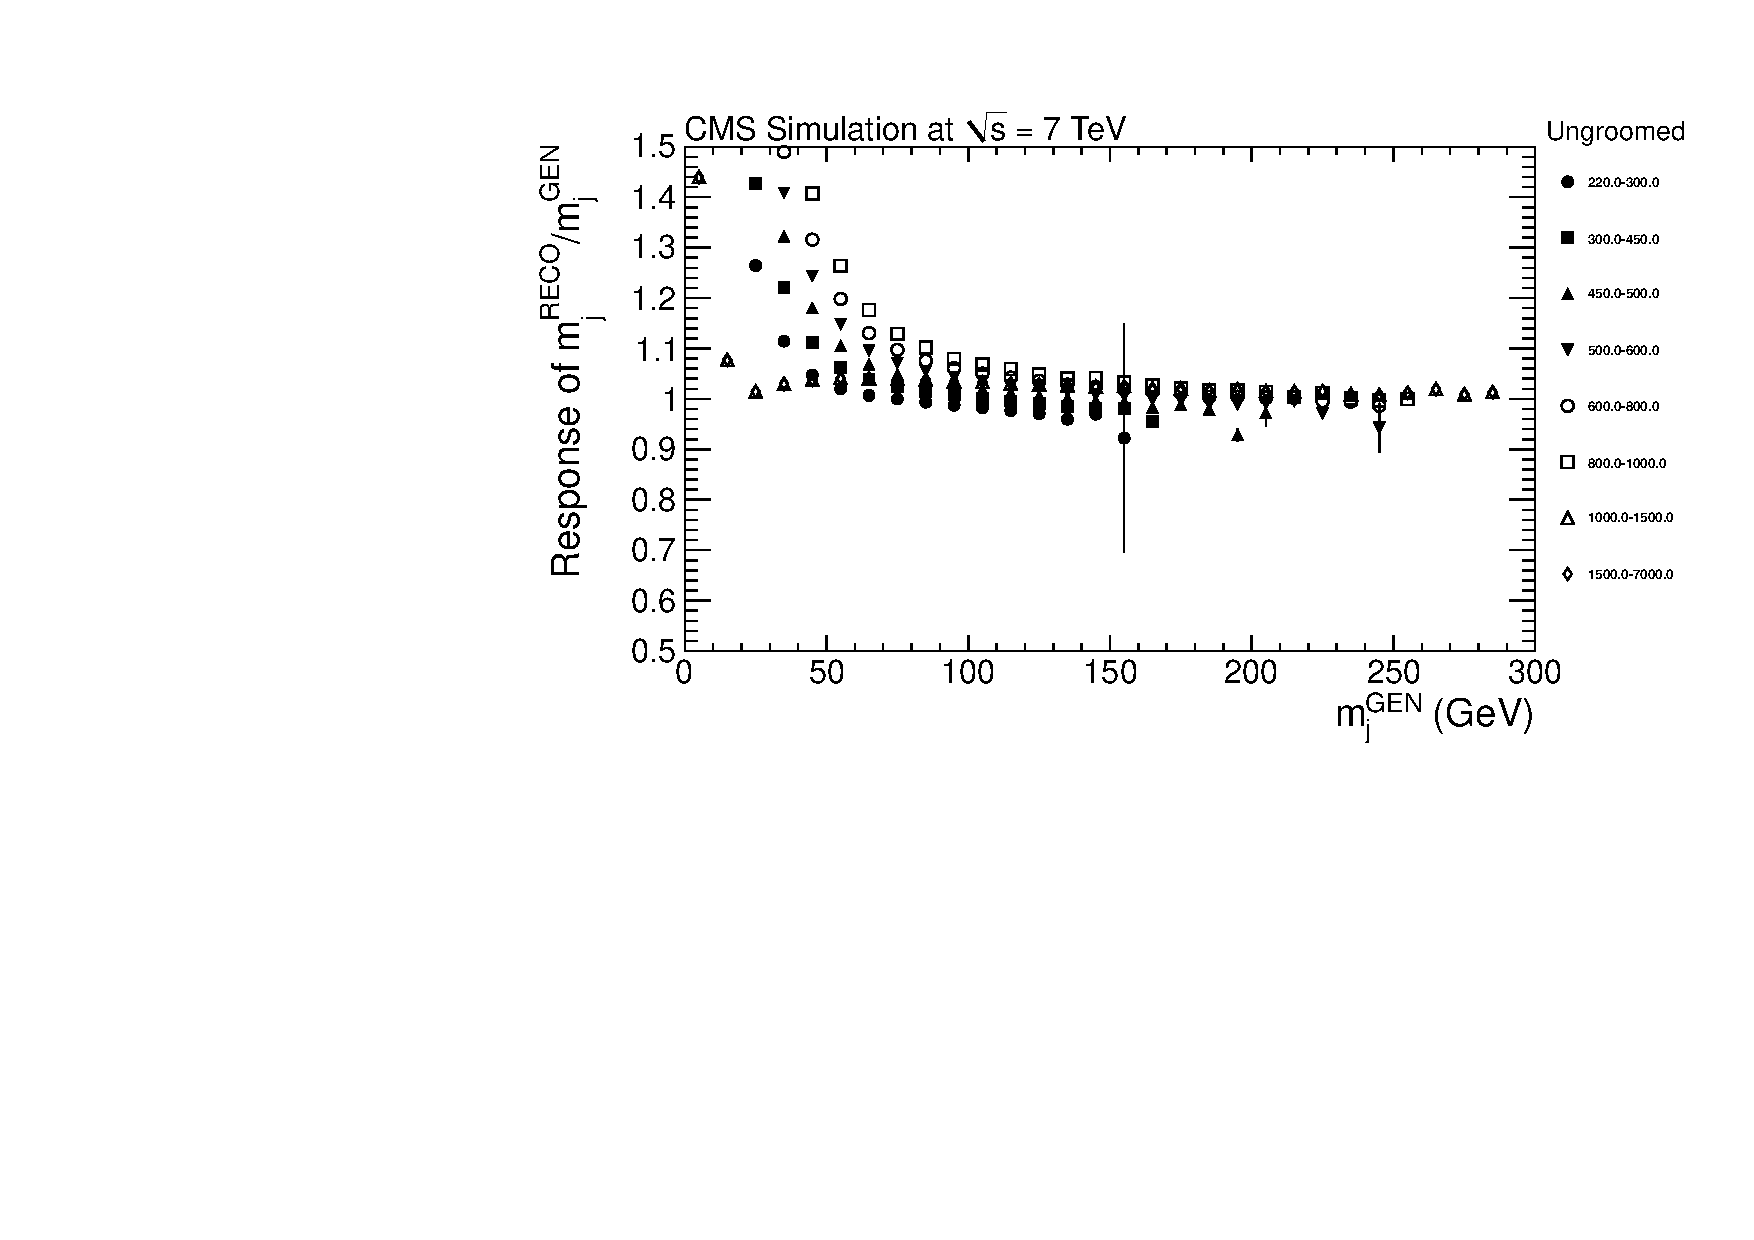
\includegraphics[width=0.5\textwidth]{figs/response_histAK7MjetResponseVsPtAvg}}
\subfigure{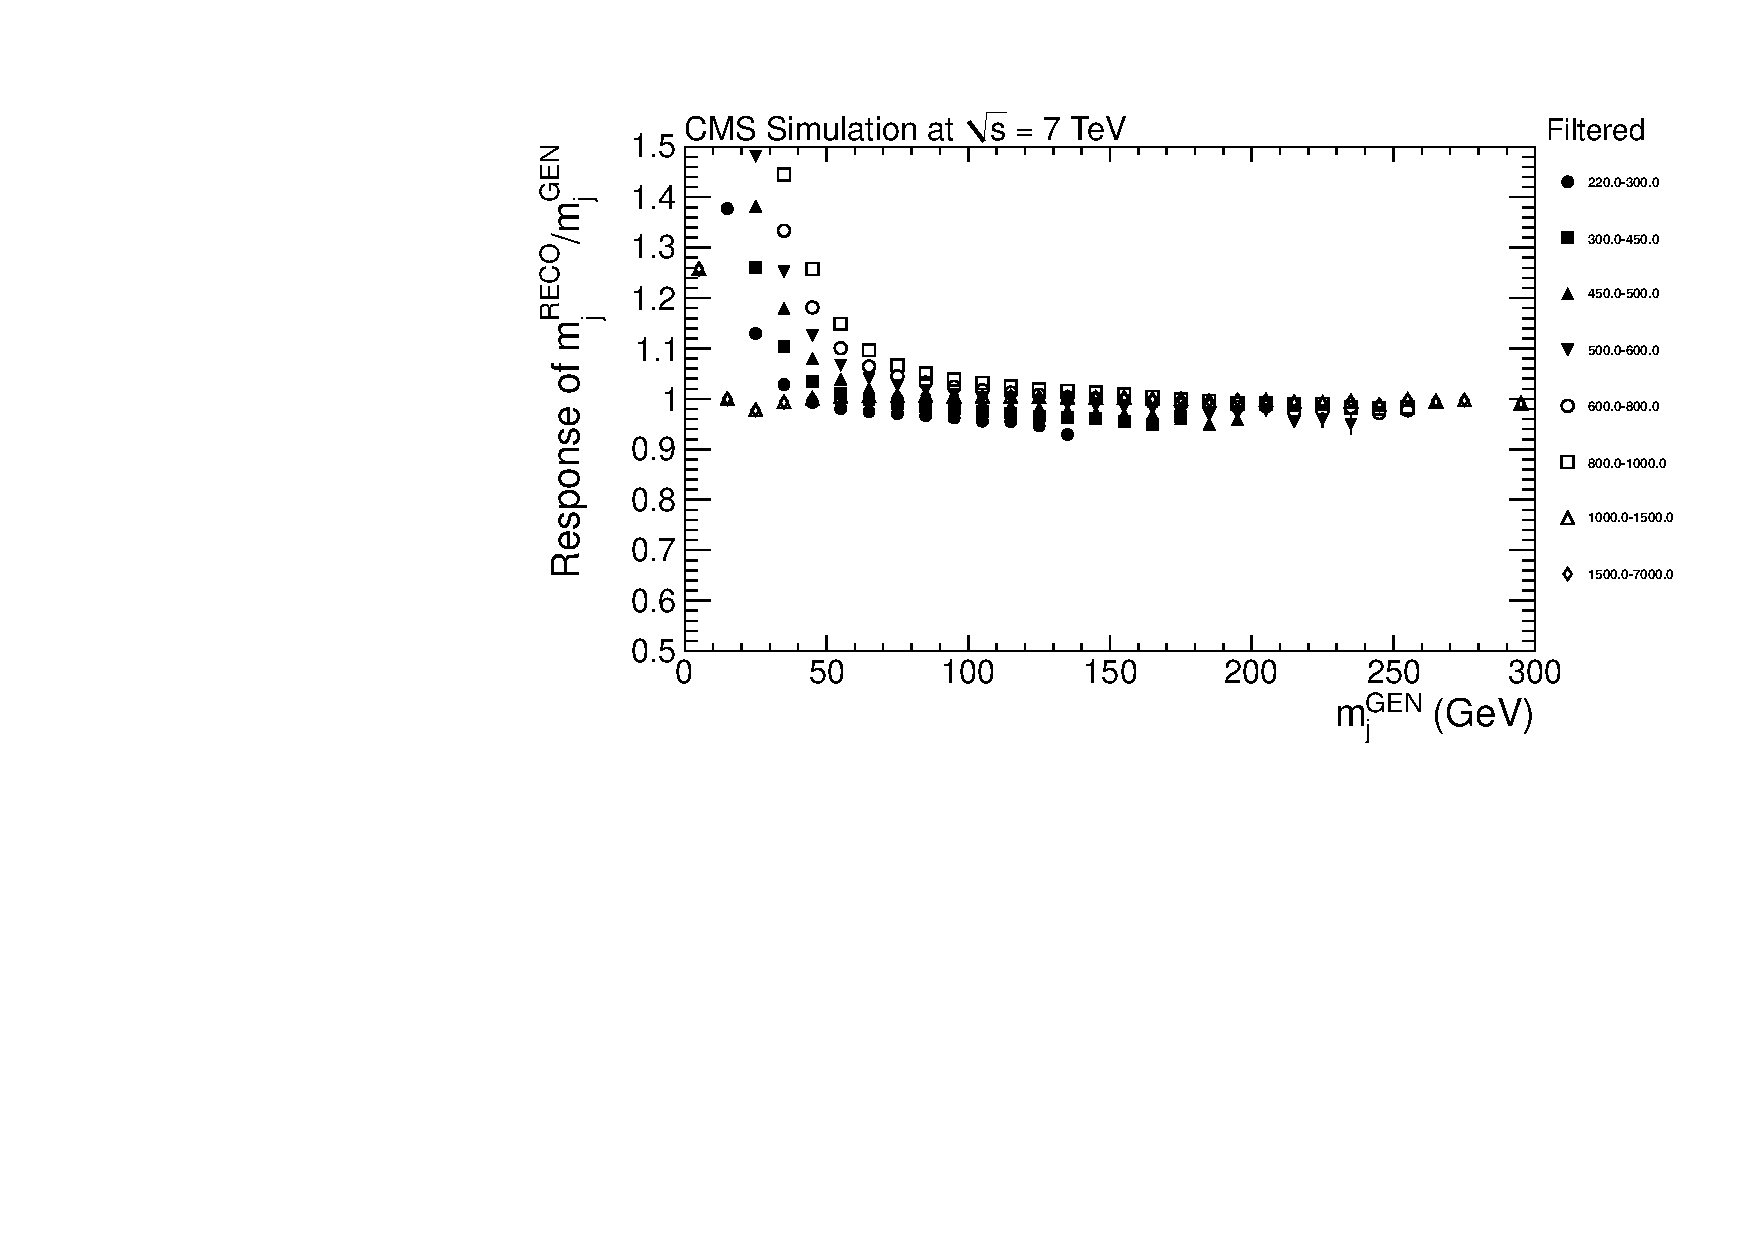
\includegraphics[width=0.5\textwidth]{figs/response_histAK7MjetResponseVsPtAvg_Filtered}}\\
\subfigure{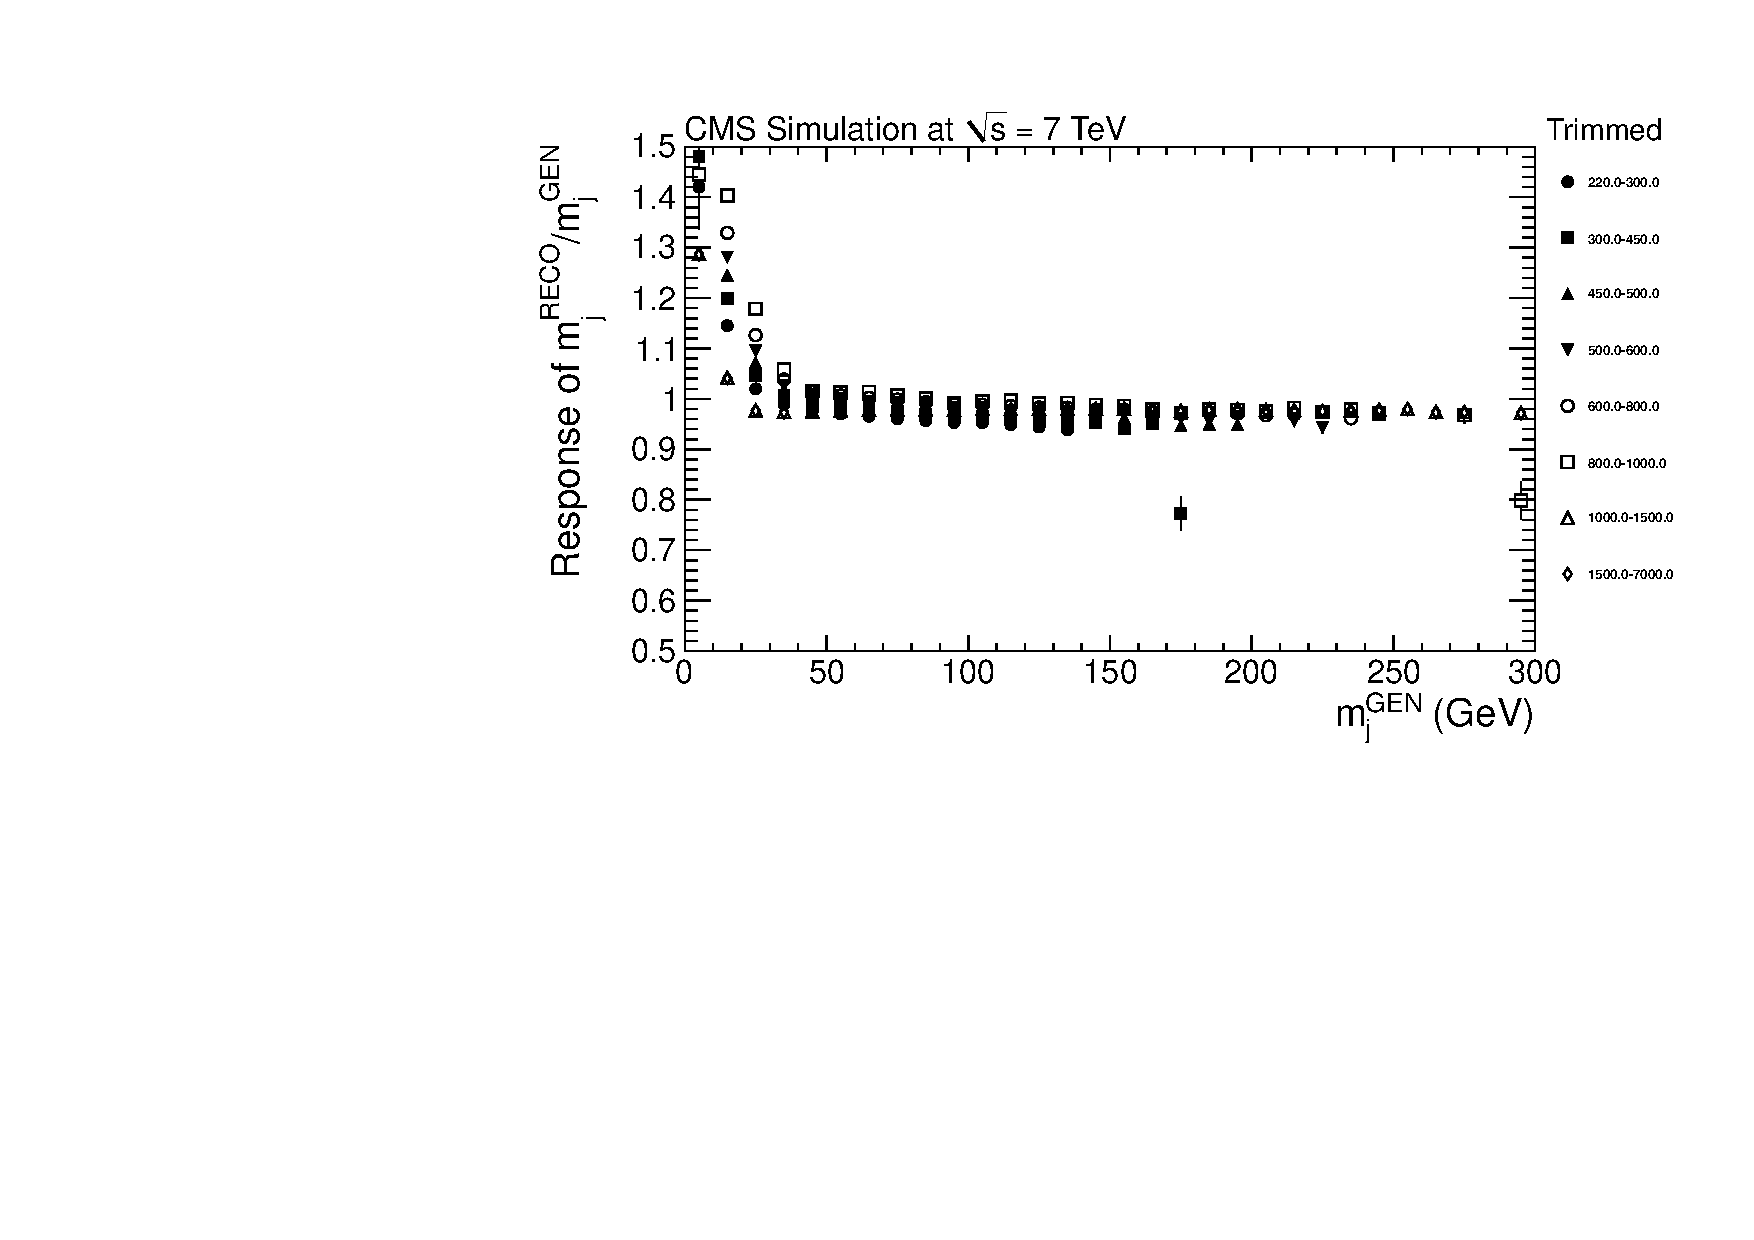
\includegraphics[width=0.5\textwidth]{figs/response_histAK7MjetResponseVsPtAvg_Trimmed}}
\subfigure{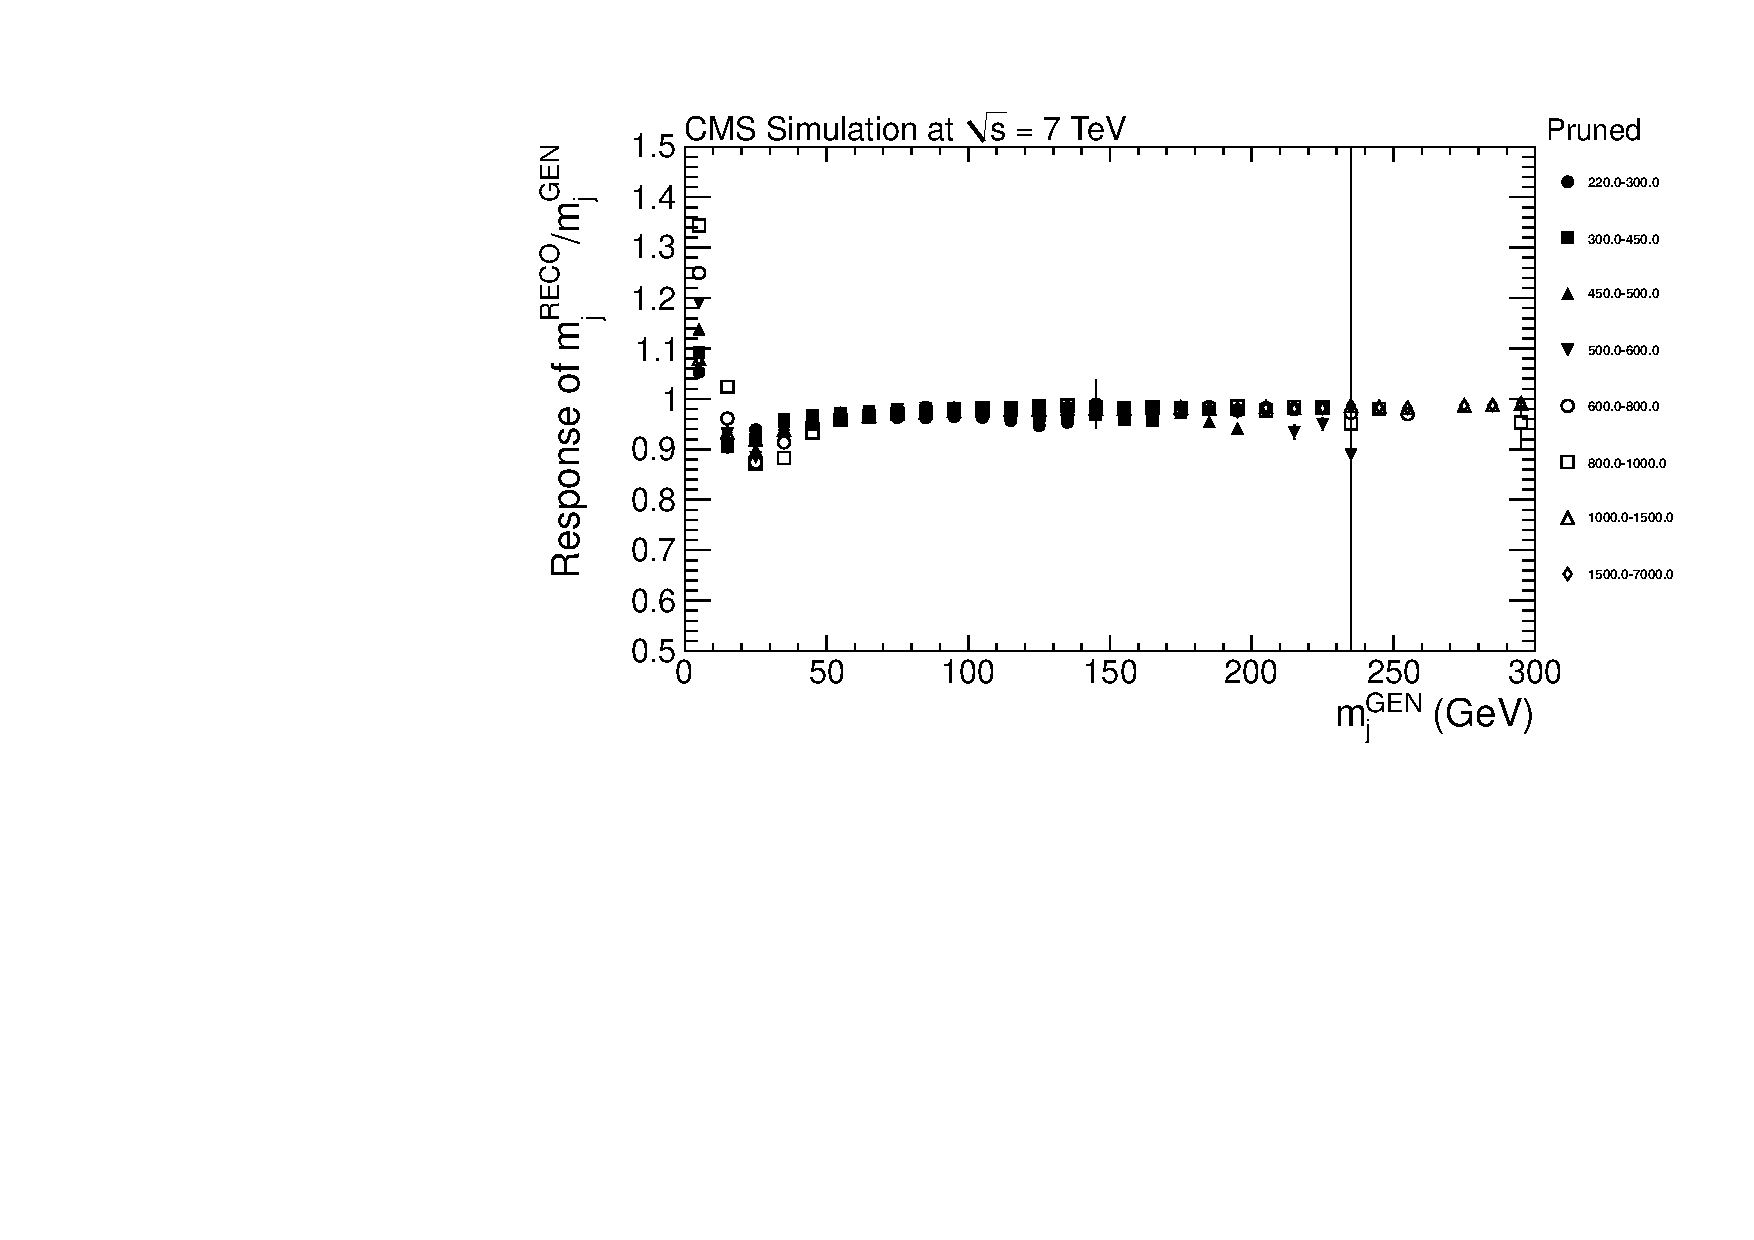
\includegraphics[width=0.5\textwidth]{figs/response_histAK7MjetResponseVsPtAvg_Pruned}}
\caption{Mean of $m_{J}^{RECO} / m_{J}^{GEN}$ in slices of 
$m_{J}^{GEN}$, for various $\pt$ bins, for each of the grooming
algorithms. This corresponds to the jet response. 
\label{figs:response_histAK7MjetResponseVsPtAvg}}
\end{figure}


\begin{figure}[htbp]
\centering
\subfigure{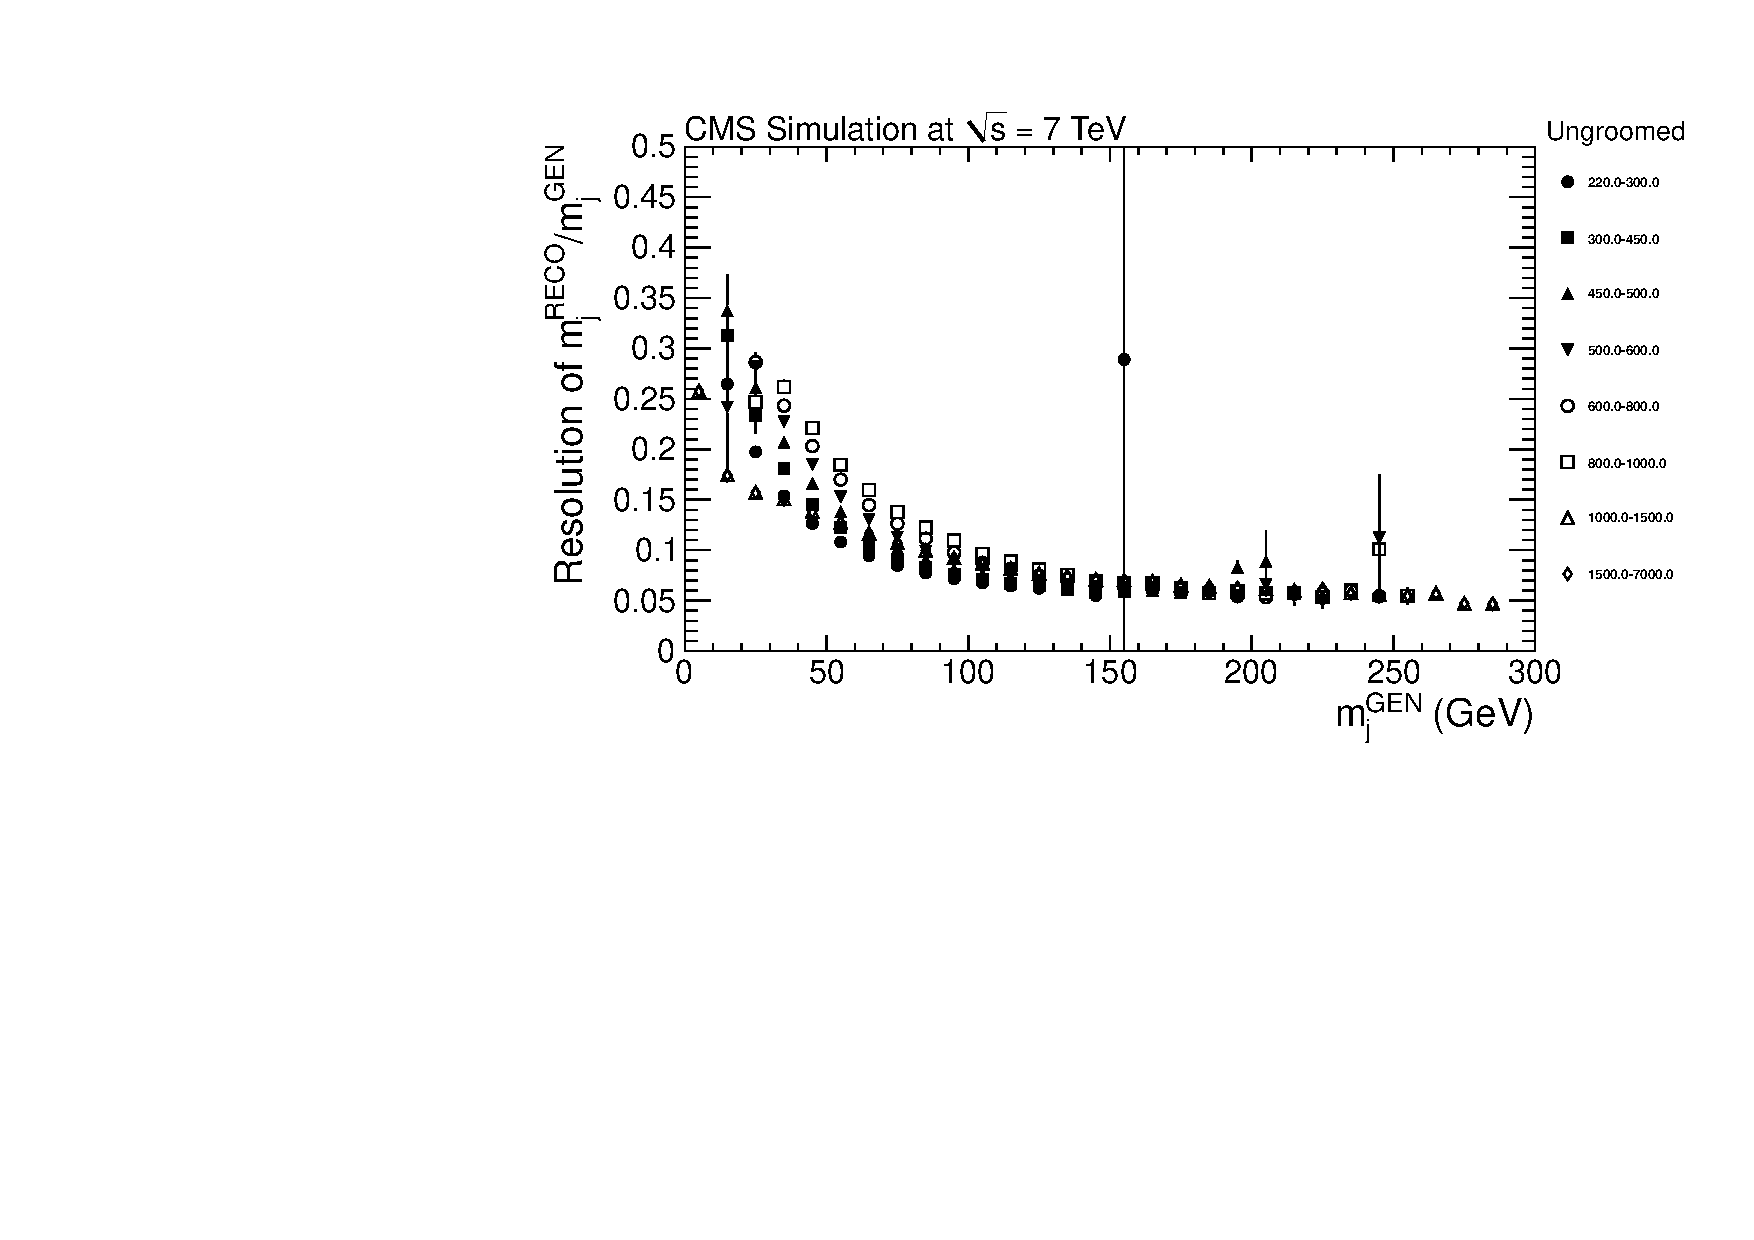
\includegraphics[width=0.5\textwidth]{figs/resolution_histAK7MjetResponseVsPtAvg}}
\subfigure{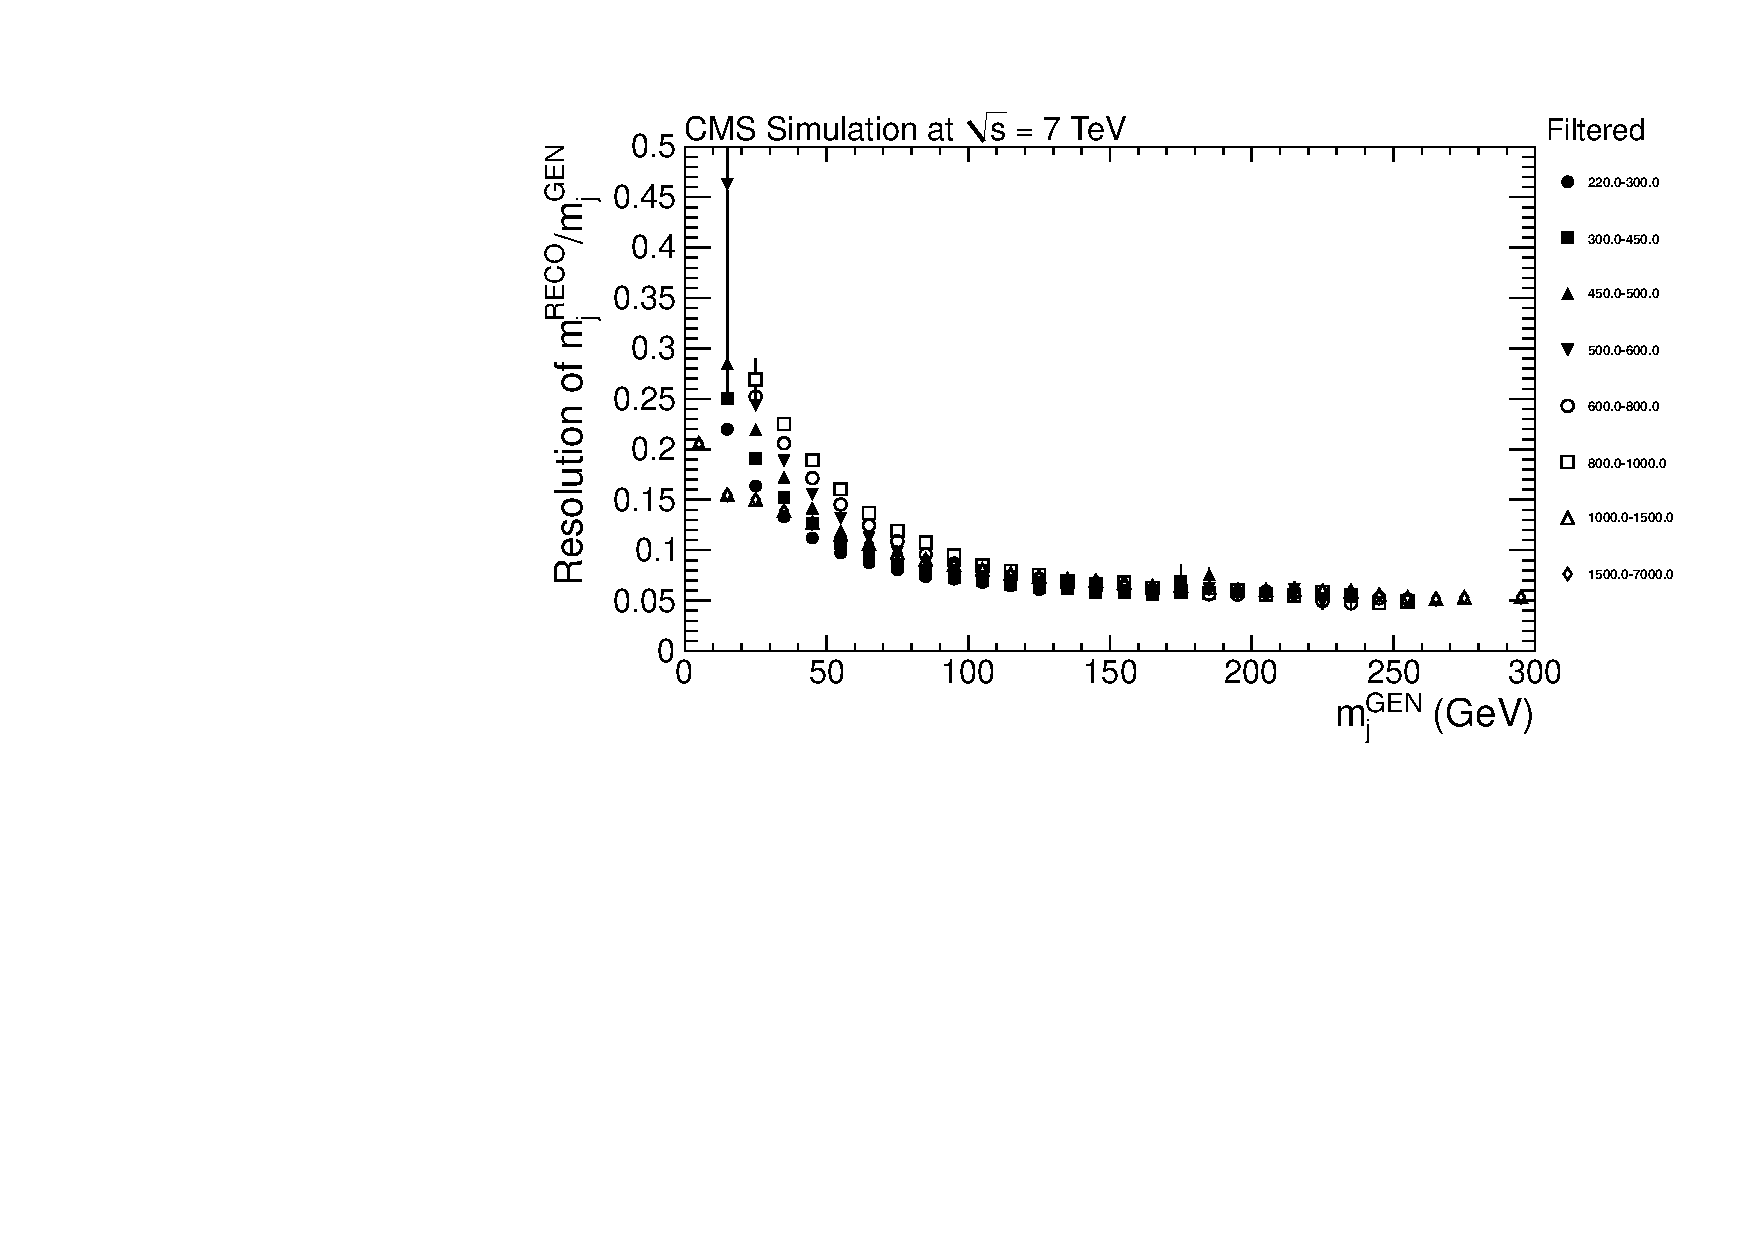
\includegraphics[width=0.5\textwidth]{figs/resolution_histAK7MjetResponseVsPtAvg_Filtered}}\\
\subfigure{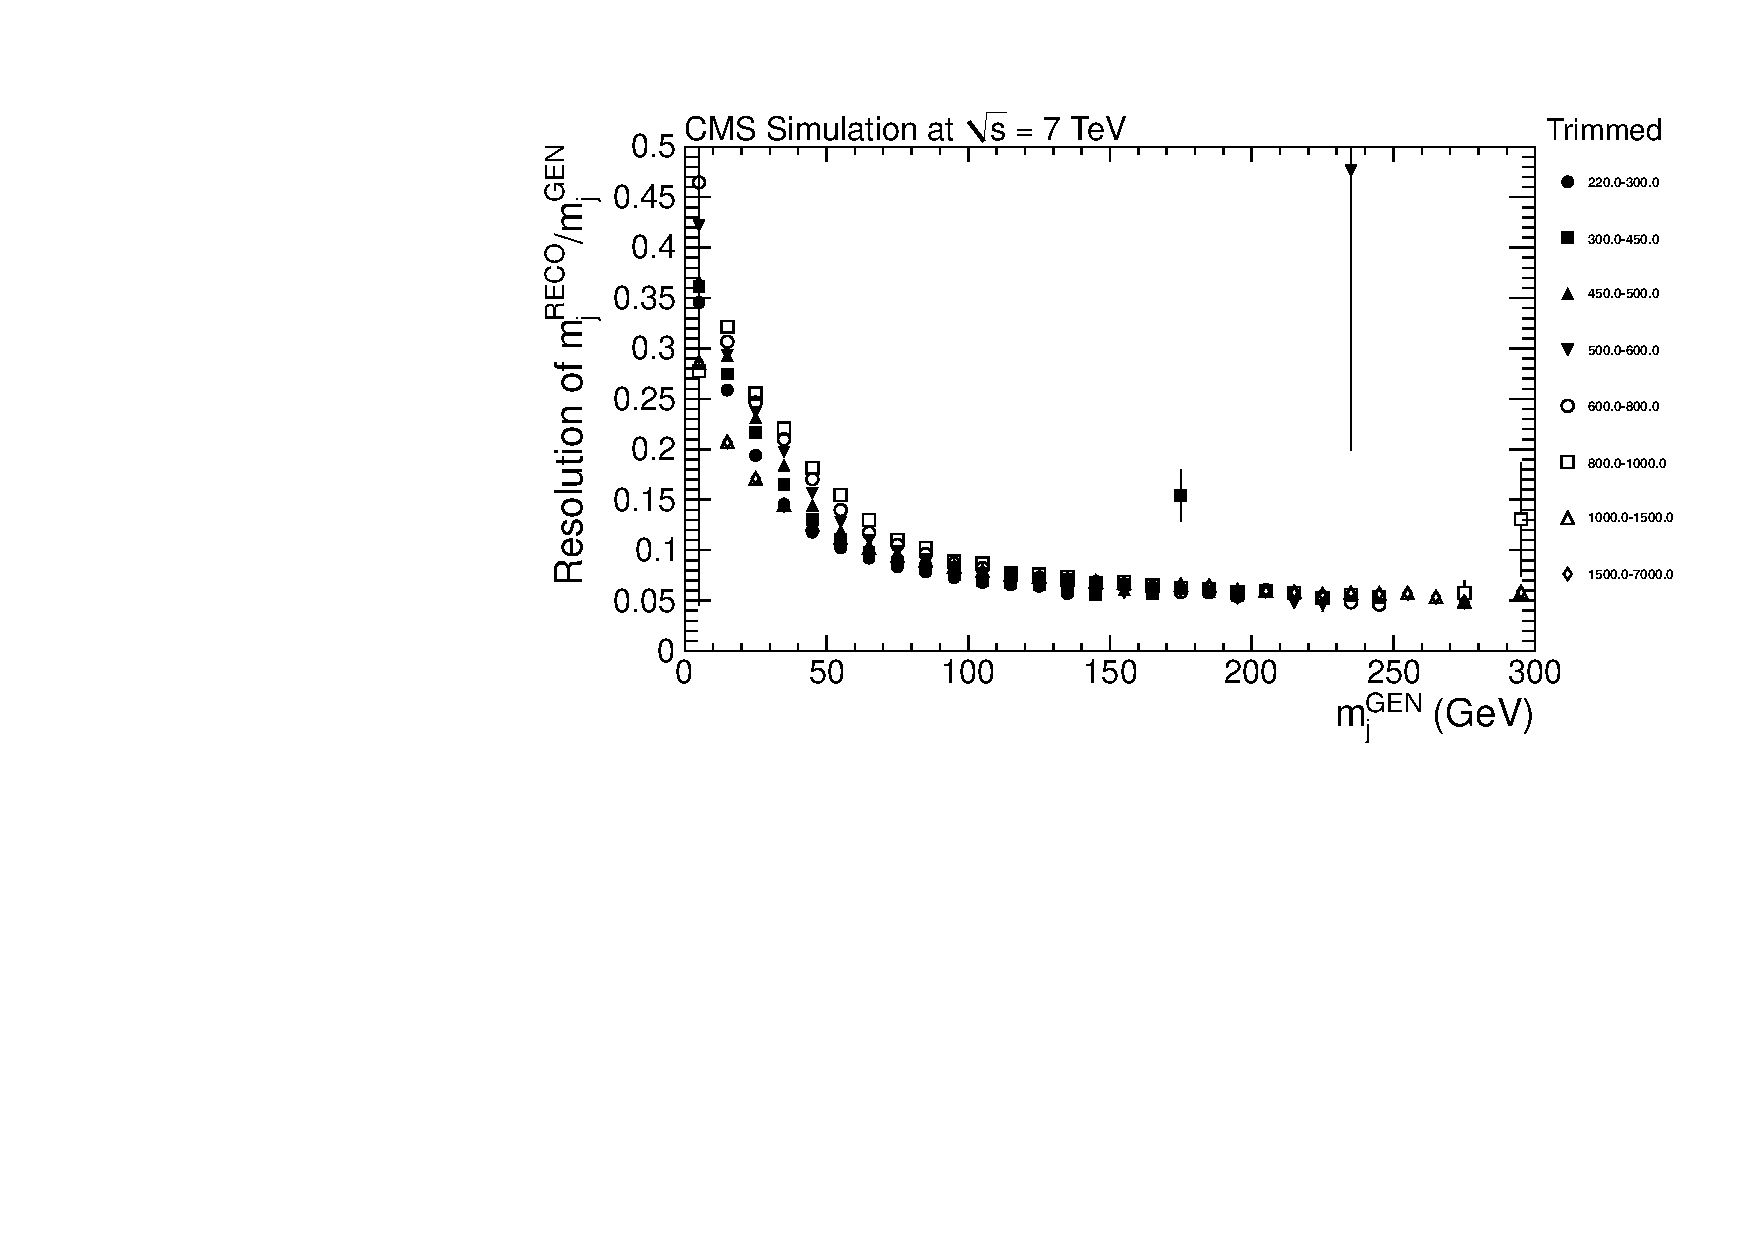
\includegraphics[width=0.5\textwidth]{figs/resolution_histAK7MjetResponseVsPtAvg_Trimmed}}
\subfigure{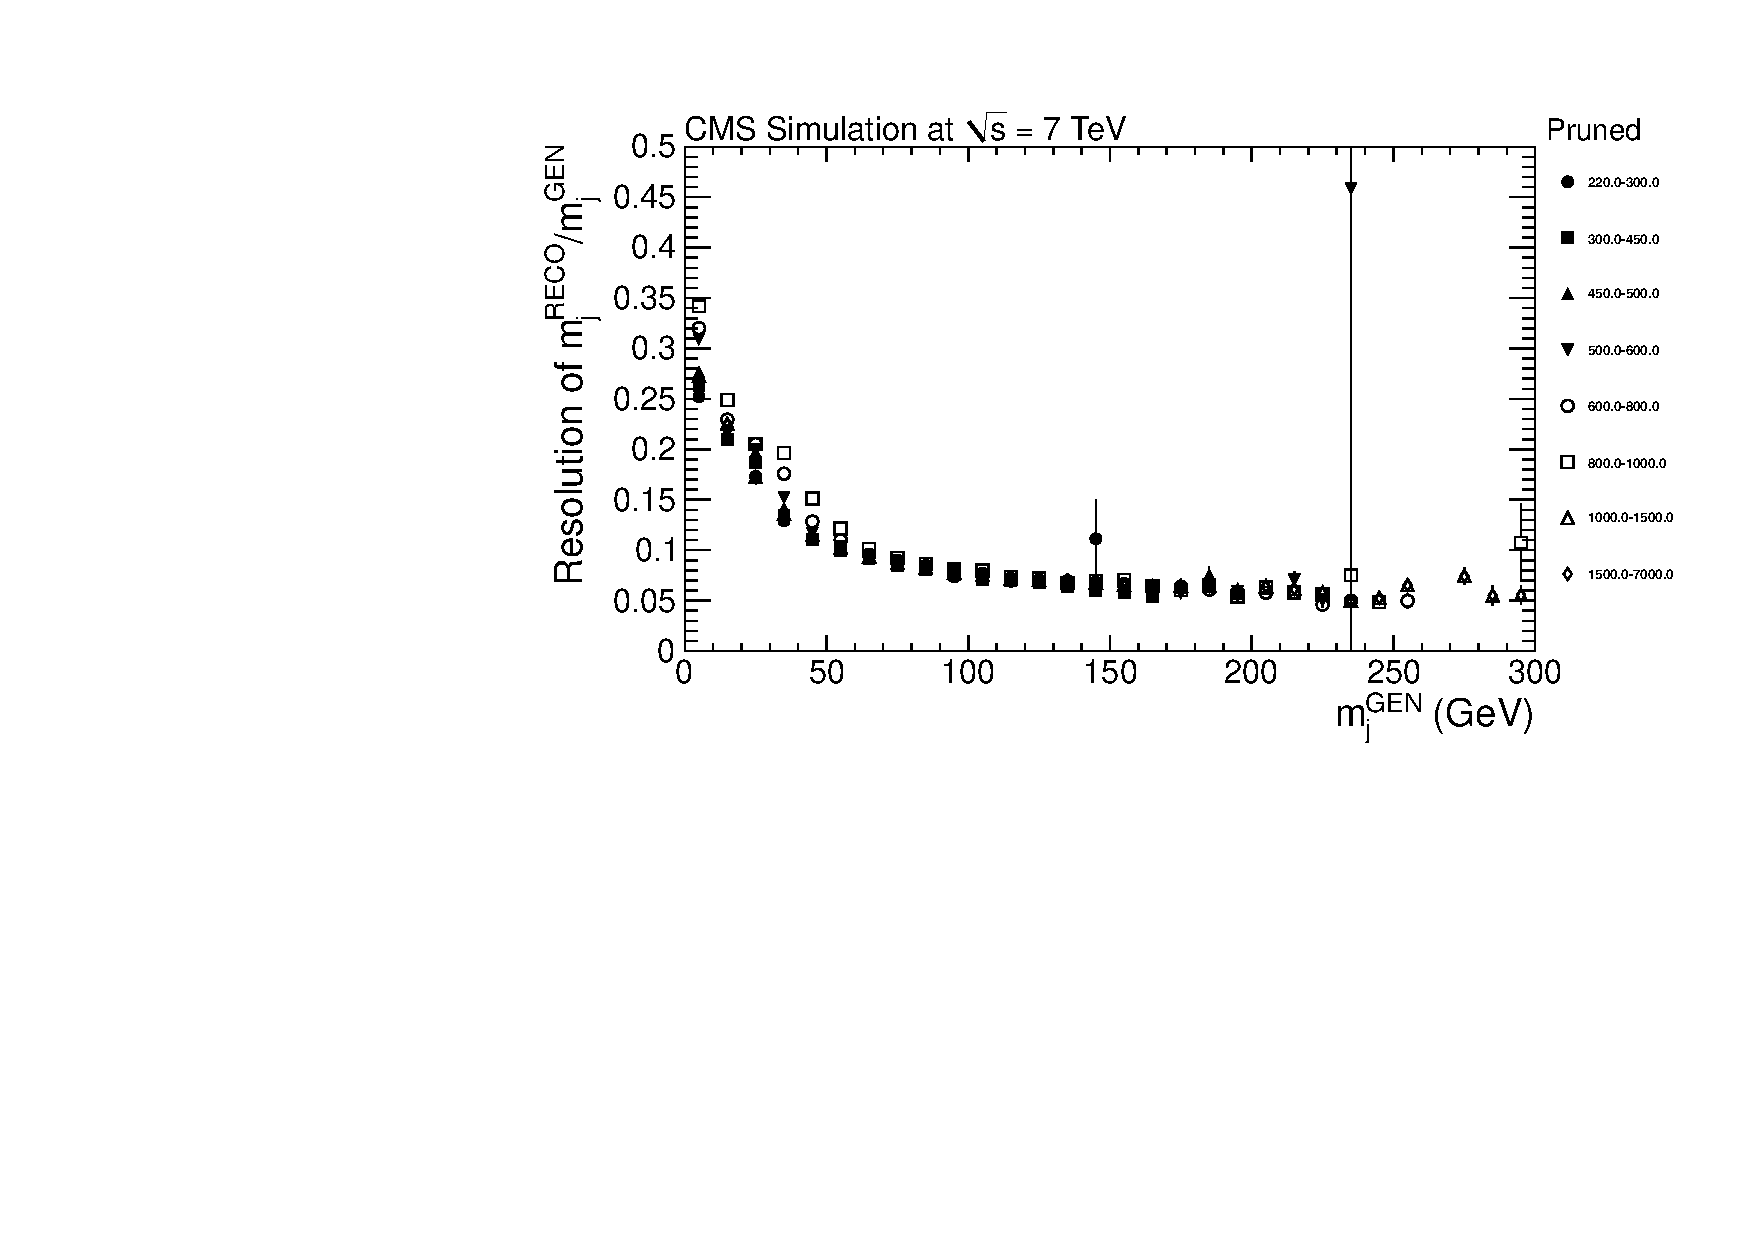
\includegraphics[width=0.5\textwidth]{figs/resolution_histAK7MjetResponseVsPtAvg_Pruned}}
\caption{Width of $m_{J}^{RECO} / m_{J}^{GEN}$ in slices of 
$m_{J}^{GEN}$, for various $\pt$ bins, for each of the grooming
algorithms. This corresponds to the jet resolution. 
\label{figs:resolution_histAK7MjetResponseVsPtAvg}}
\end{figure}


\subsection{Trigger assignment}
\label{sec:trigAssignment}

The triggers that were used in this analysis have partially overlapping phase space. 
The lower-threshold triggers have high prescales in order to accommodate higher
trigger rates, and the $\pt$ selections on these triggers are only one-sided,
hence lower-threshold triggers have overlapping phase space with higher-threshold
triggers. To correctly assign events to a specific trigger, the
strategy used is to compute the trigger efficiency as a function
of $\pt^{AVG}$ and select a region in the trigger plateau, then
assign one trigger per $\pt^{AVG}$ region. Table~\ref{TriggerTurnOns}
shows the trigger threshold for each trigger.
Figure~\ref{figs:efficiency_HLT}
shows the efficiency turn-ons computed with respect to the
next lowest trigger. The efficiency is defined as:

\begin{equation}
\epsilon = \frac{L_{A-1} N_{A}}{L_{A} N_{A-1}}
\end{equation}

where $\epsilon$ is the efficiency, $N_{A}$ is the number of
events that pass trigger with threshold $A$, and $L_{A}$ is the
effective luminosity of the trigger with threshold $A$ as shown
in Tab.~\ref{fig:trigger}. 


In the case of using
groomed jets, the trigger assignment is still used from the ungroomed
collection, and hence the trigger assignment is identical for all
algorithms, whether or not they are groomed. 
The trigger binning is selected such that the efficiency is in the
plateau. 

\begin{figure}[htbp]
\centering
\subfigure{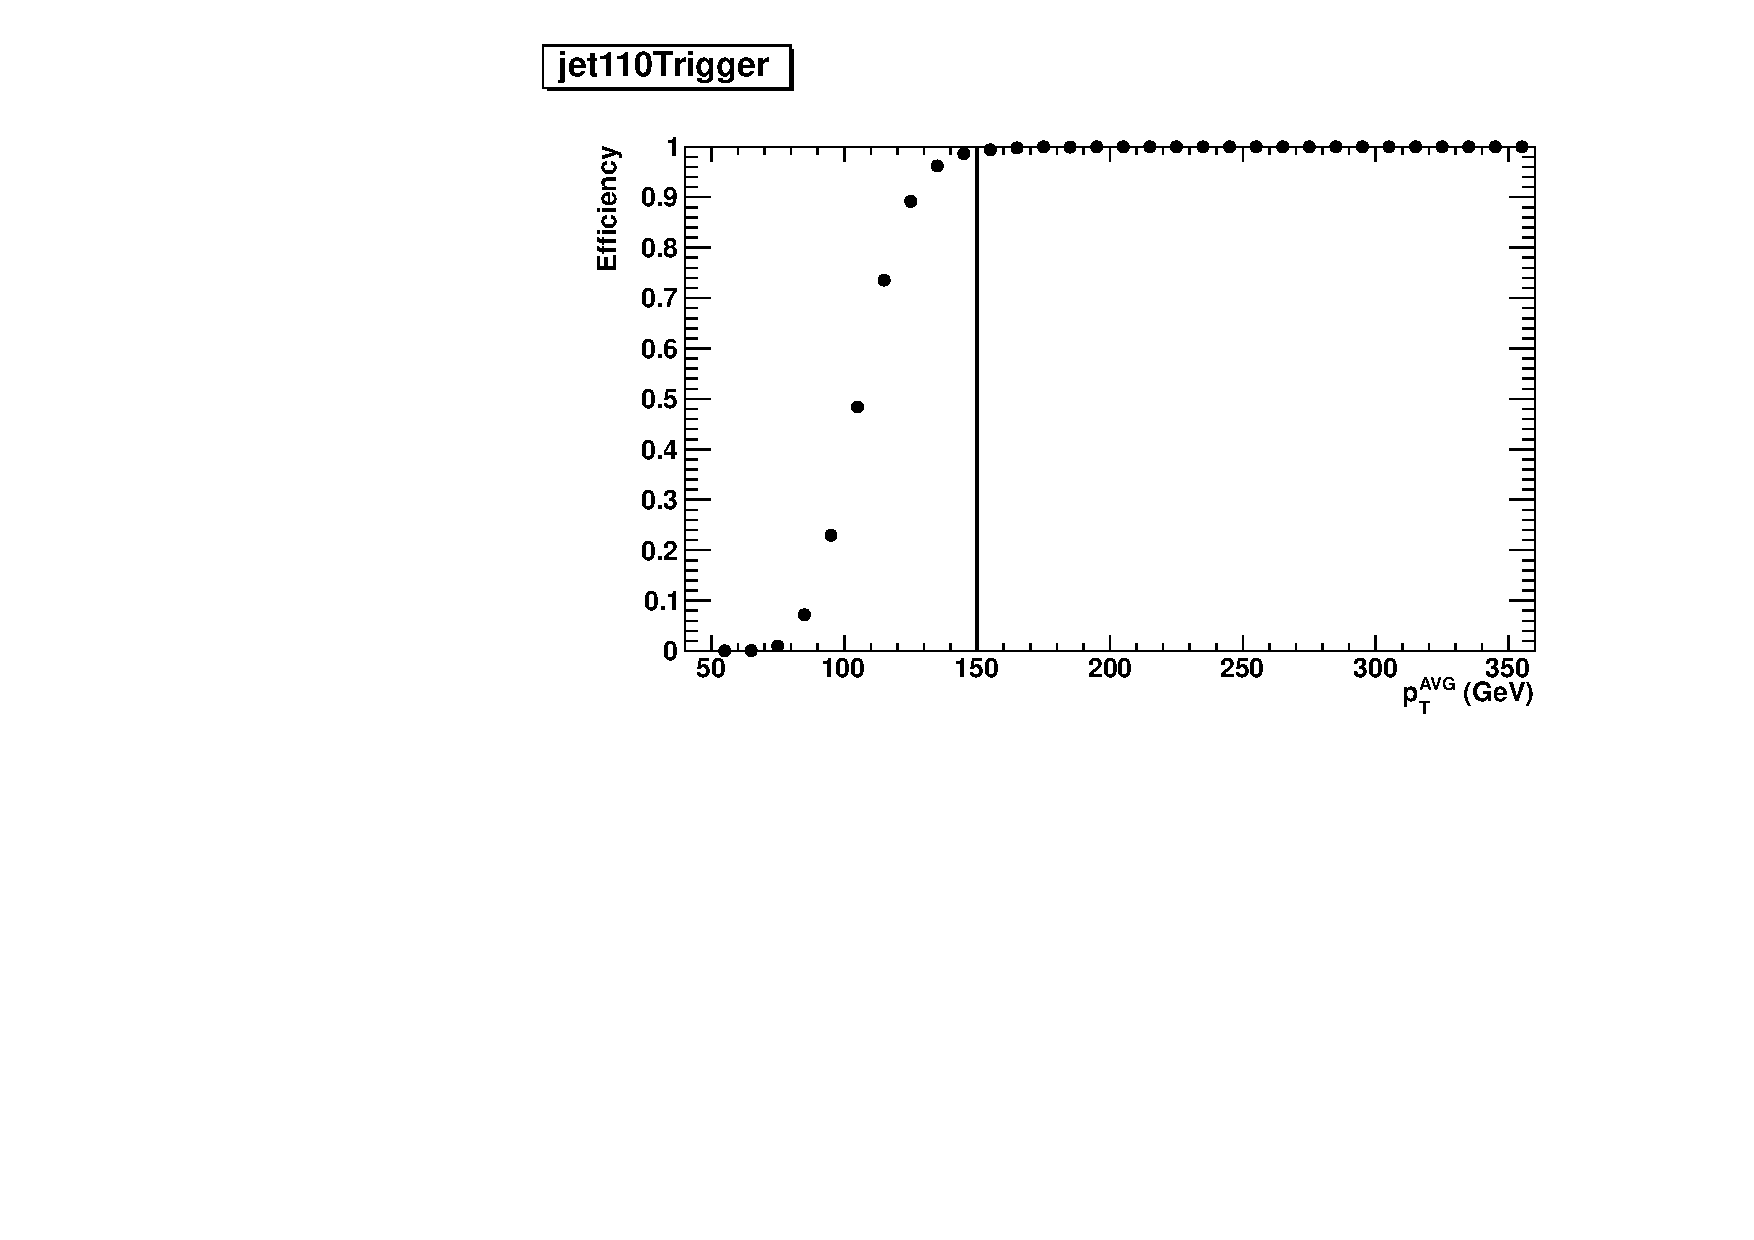
\includegraphics[width=0.6\textwidth]{figs/efficiency_jet110Trigger}}
\subfigure{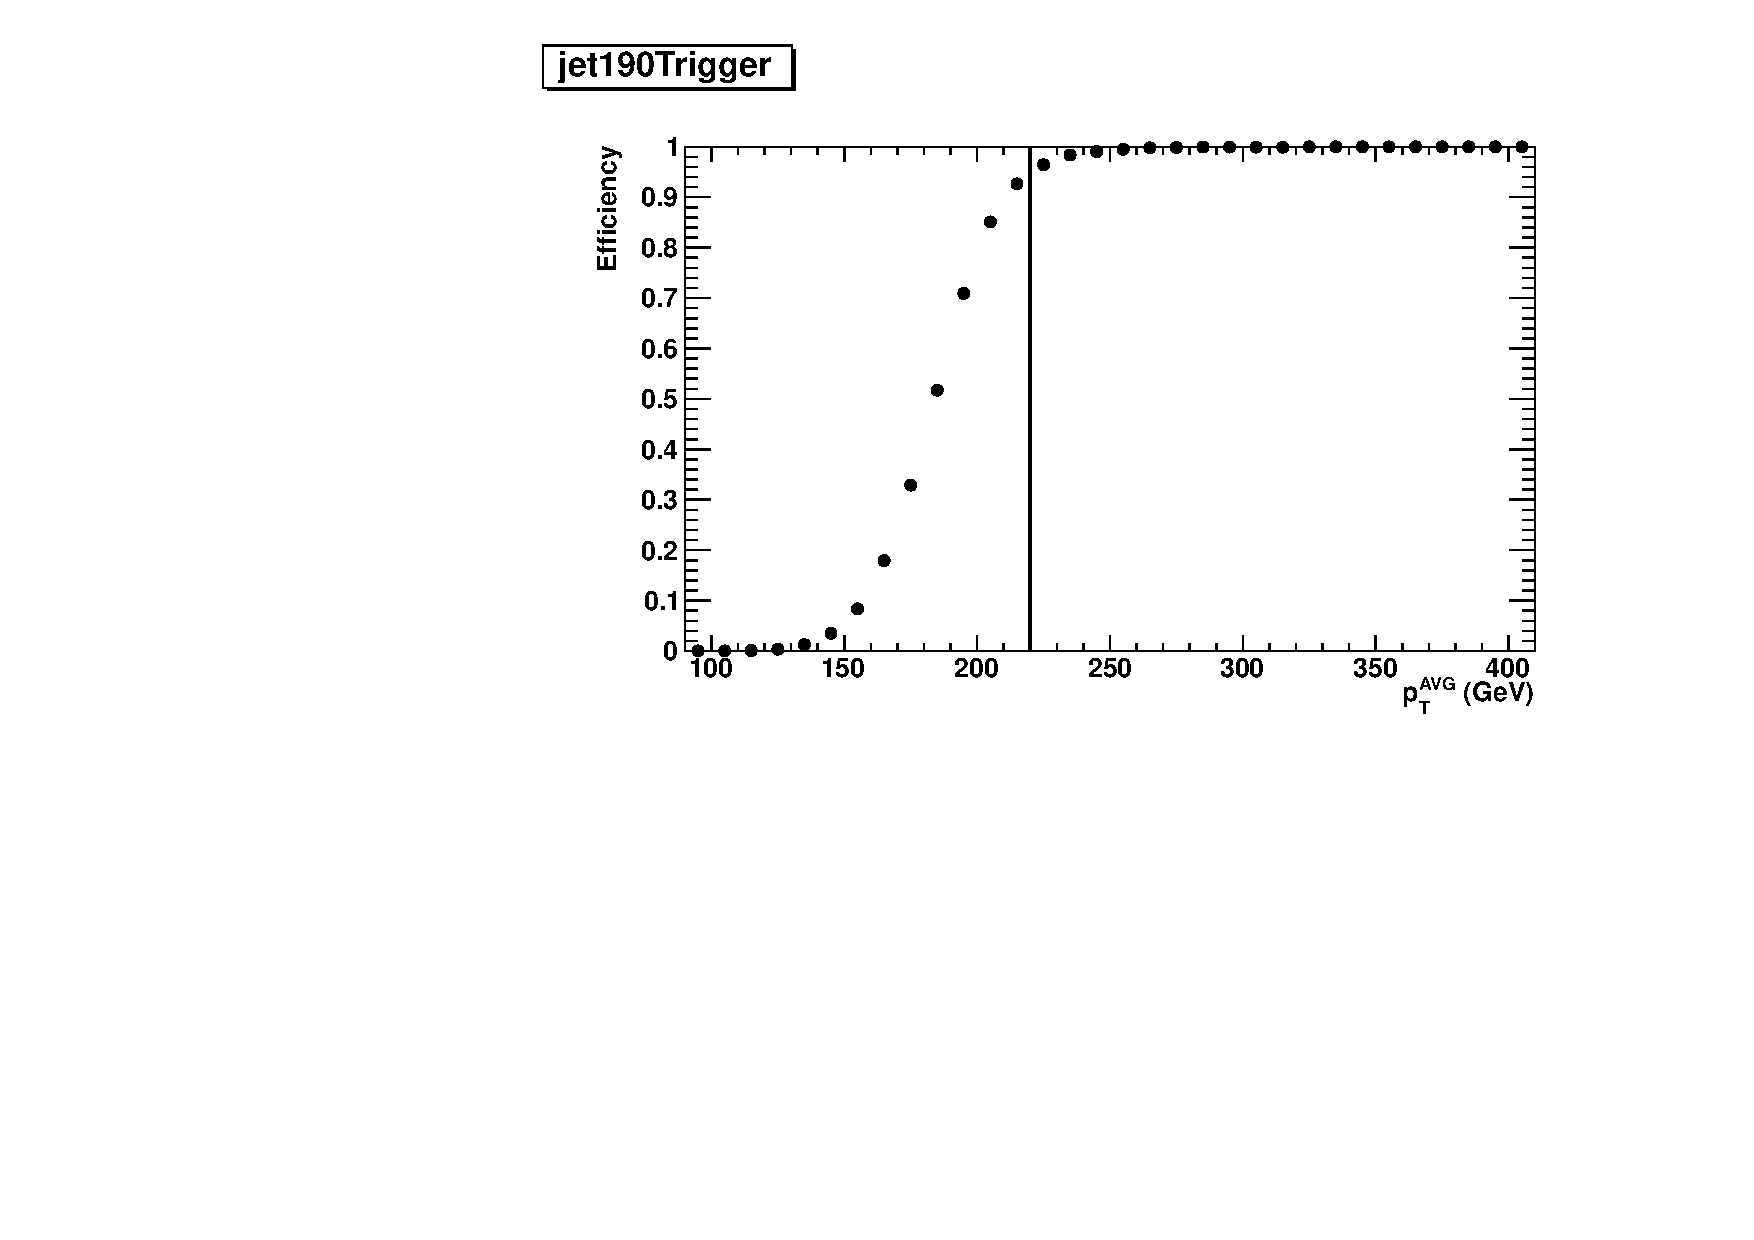
\includegraphics[width=0.6\textwidth]{figs/efficiency_jet190Trigger}}\\
\subfigure{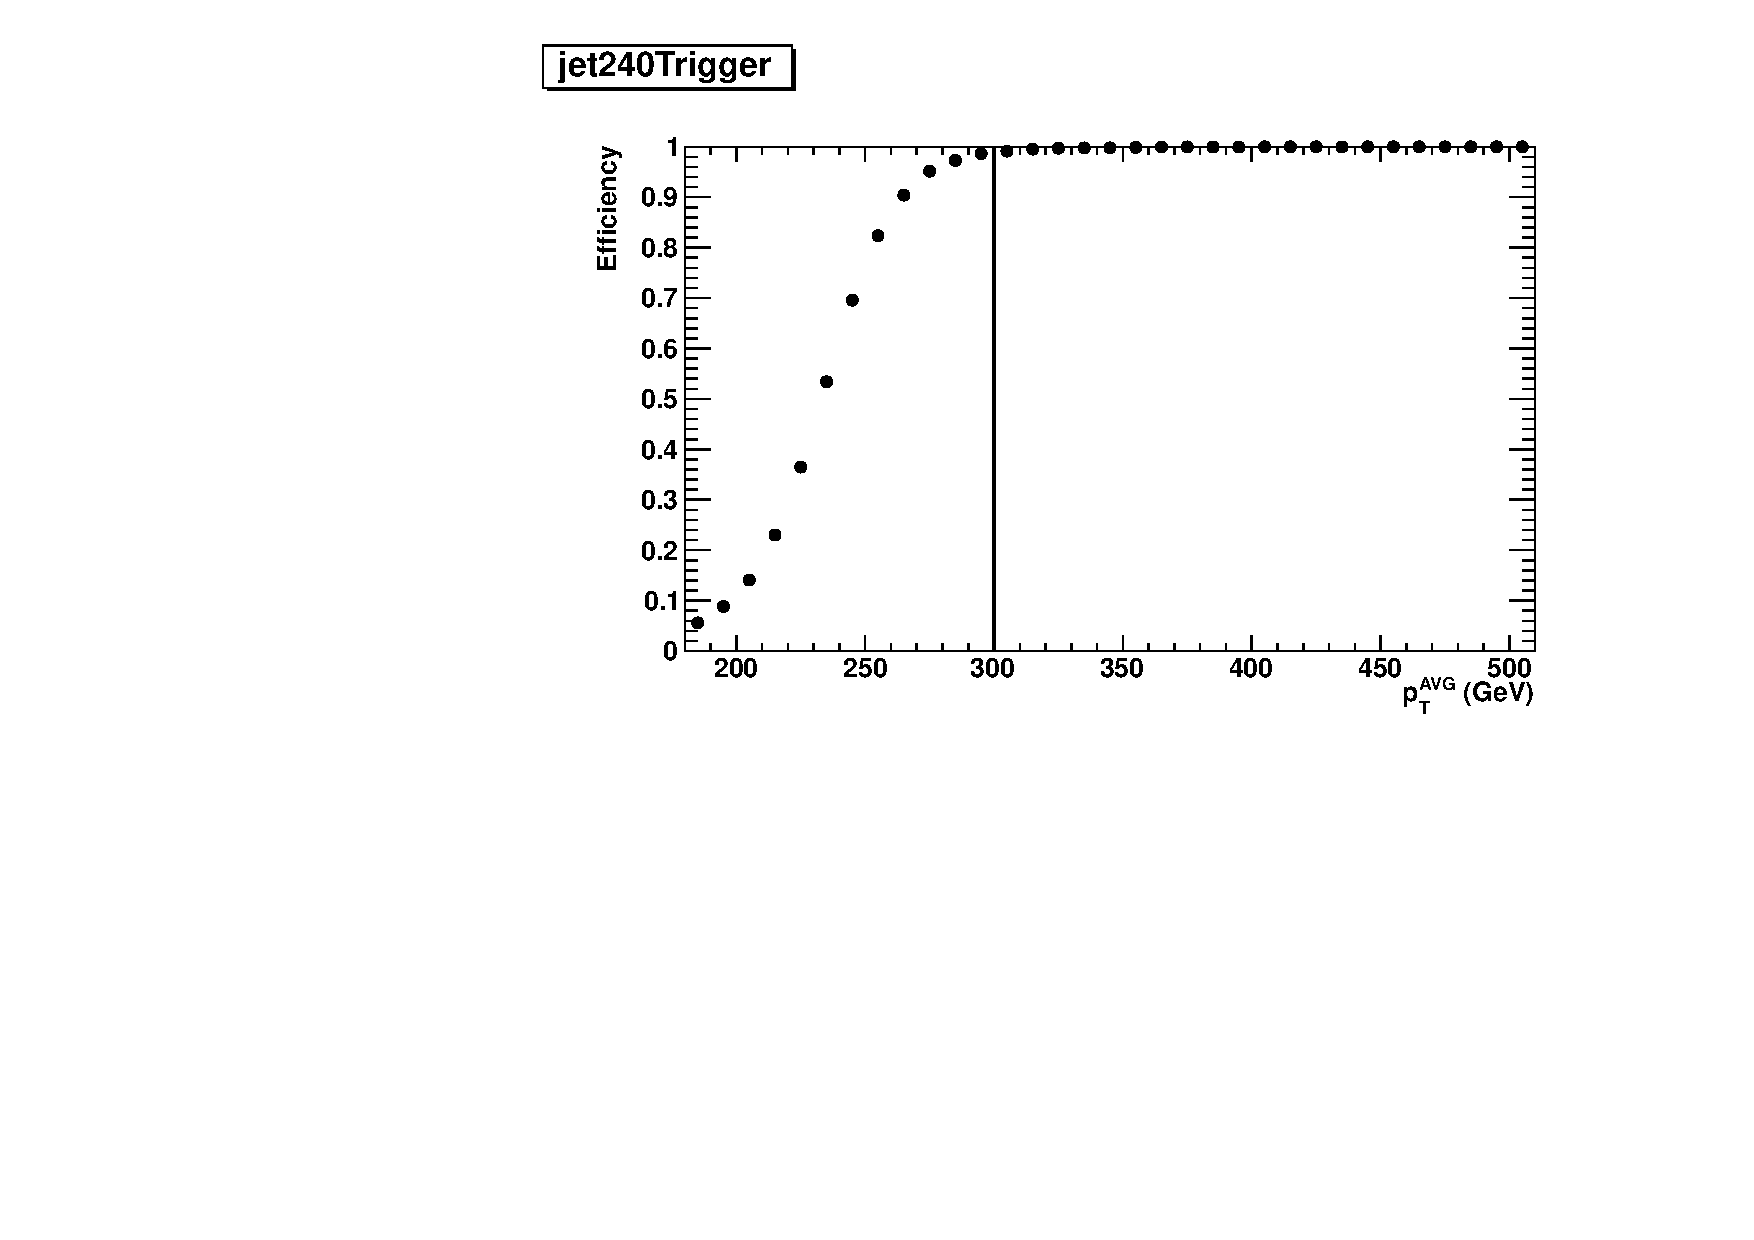
\includegraphics[width=0.6\textwidth]{figs/efficiency_jet240Trigger}}
\subfigure{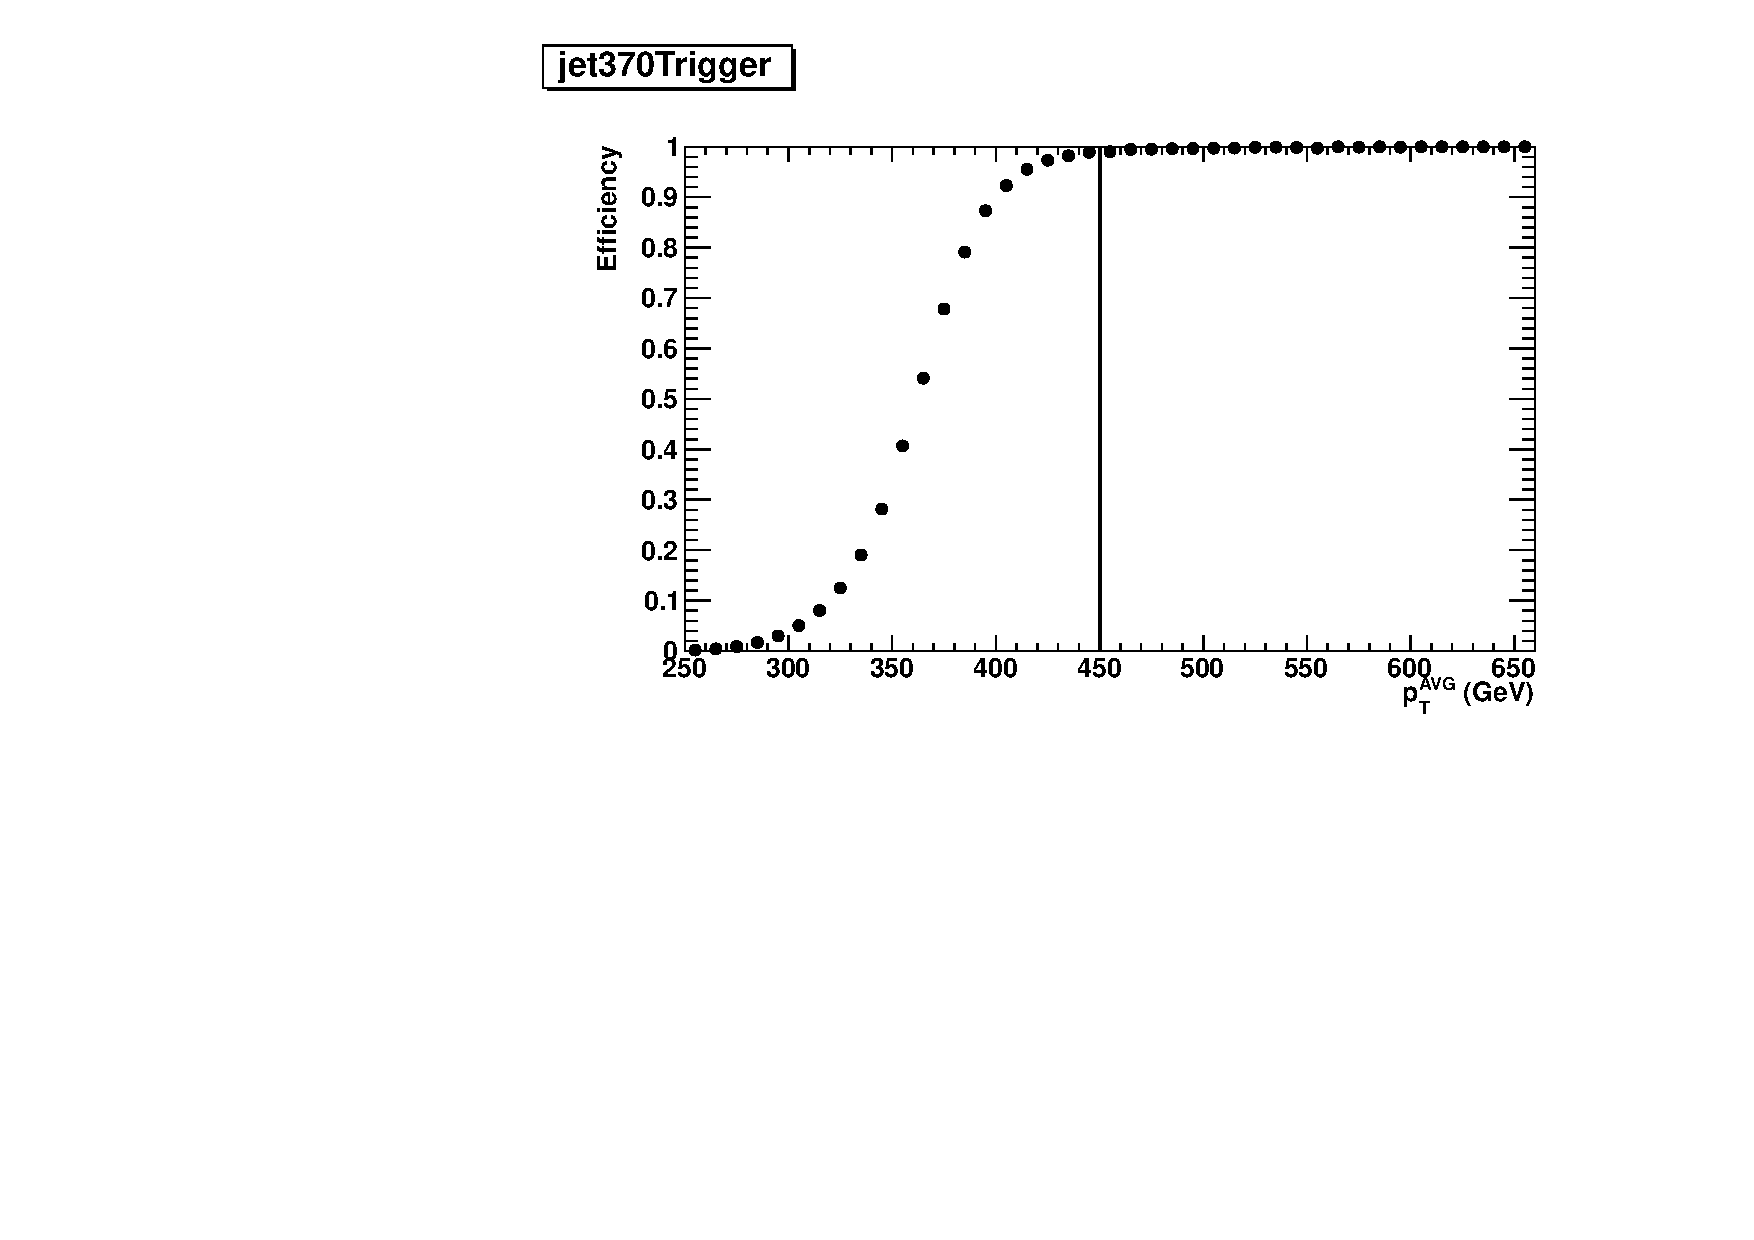
\includegraphics[width=0.6\textwidth]{figs/efficiency_jet370Trigger}}
\caption{Trigger efficiency as a function of $\pt^{AVG}$. 
\label{figs:efficiency_HLT}}
\end{figure}


\begin{table}[h]
  \centering
  \begin{tabular}{ |c|c|}
    \hline 
Jet60 & 0-150 \GeV   \\
Jet100& 150-220 \GeV \\
Jet190& 220-300 \GeV \\
Jet240& 300-450 \GeV \\
Jet370& $>$450 \GeV \\
   \hline 
  \end{tabular}
  \caption{Trigger efficiency turn-on values for all jet samples.\label{TriggerTurnOns}}
\end{table}



\subsection{Transverse momentum bin assignment}
\label{sec:ptBinAssignment}


The jet mass is correlated with the energy of the jet. As such,
it is necessary to measure the jet mass in bins of transverse 
momentum of the jet $\pt$. Since this analysis uses a dijet
sample, the average jet $\pt$ is used as a variable of interest ($\pt^{AVG}$).

The $\pt^{AVG}$ binning chosen is to be
as similar as possible to the V+Jets analysis in
Ref~\cite{cmsSMPJSVJ}.
It is also chosen such that only one dijet trigger contributes to each
bin in $\pt^{AVG}$. 
As such, the binning is shown in Table~\ref{tab:ptBins}.
In this case, to assure that the appropriate $\pt$ dependence
of the jet mass is captured for the various grooming algorithm,
the $\pt^{AVG}$ is evaluated for each of the grooming techniques. 


\begin{table}[h]
  \centering
  \begin{tabular}{ |c|c|}
    \hline 
    Bin & $\pt^{AVG}$ \\ 
    \hline
    %0 & 0-50 \GeVc \\
    1 & 50-125 \GeVc \\
    2 & 125-150 \GeVc \\
    3 & 150-220 \GeVc \\
    4 & 220-300 \GeVc \\
    5 & 300-450 \GeVc \\
    6 & 450-500 \GeVc \\
    7 & 500-600 \GeVc \\
    8 & 600-800 \GeVc \\
    9 & 800-1000 \GeVc \\
    10& 1000-1500 \GeVc \\
    11& $>$1500 \GeVc \\
    \hline 
  \end{tabular}
  \caption{Jet $\pt^{AVG}$ bins. \label{tab:ptBins}}
\end{table}

\clearpage

\section{Data/MC raw comparisons}
\label{sec:rawDataMCComparisons}

In this Section, the detector-level distributions of the jet mass
are investigated. Each of the distributions are made for 
the $\pt^{AVG}$ bins described in Section~\ref{sec:ptBinAssignment}. 
Each of the figures shows the raw event counts per $\pt^{AVG}$ bin,
as a function of the average jet mass $m_J^{AVG}$. 


Figure~\ref{figs:histAK7PtAvgVsMjetGroomOverReco_ratioPlots}
shows a comparison of the jet mass from the groomed jets
divided by the jet mass of matched ungroomed jets, for the
three grooming techniques, for both data and the \PYTHIA Monte Carlo. 
The data and the MC both exhibit similar behavior. In general,
the filtering algorithm (black) is the least aggressive grooming technique,
with groomed jet masses close to the ungroomed case.
The trimming algorithm (red) is moderately aggressive, and the
pruning algorithm (blue) is the most aggressive. In the case of
the pruning algorithm, a bimodal distribution begins to manifest,
which is typical of this algorithm since the parameters we have
chosen require two subjets to be created. In the cases where
the pruned jet mass is close to the ungroomed jet mass, 
jets usually have large ``core'' components
and small amounts of radiation, whereas when the pruned jet
mass is closer to 0, the jets are more symmetrically split
due to gluons splitting into two jets that fall within
our $D=0.7$ parameter. 


Figures~\ref{figs:controlPlots_histAK7PtAvgVsNvtx} and \ref{figs:controlPlots_histAK7DeltaPhi}
show the $\pt^{AVG}$ and $\Delta \phi$ distributions for the data
compared to the \PYTHIA MC. The $\pt^{AVG}$ distribution is reasonably
well-modeled with the \PYTHIA MC, but the $\Delta \phi$ distribution
does show some mismodeling.

Figures~\ref{figs:histAK7MjetVsPtAvg_rawDataMCComparisons_stacktrigs_pt_1}-
\ref{figs:histAK7MjetVsPtAvg_rawDataMCComparisons_stacktrigs_pt_10}
show the jet mass distribution for AK7 jets, along with
the trigger breakdown for all of the $\pt^{AVG}$ bins. In each case,
only one trigger contributes to any given $\pt^{AVG}$ bin. 

Figures~\ref{figs:histAK7MjetVsPtAvg_rawDataMCComparisons_pt_1}-
\ref{figs:histAK7MjetVsPtAvg_rawDataMCComparisons_pt_10_Pruned}
show the detector-level distributions for the various jet grooming
algorithms, compared to predictions from \PYTHIA, \PYTHIA8, and
\HERWIG Monte Carlo samples. Each MC sample is normalized
according to the expected luminosity and computed cross sections. 



\begin{figure}[htbp]
\centering
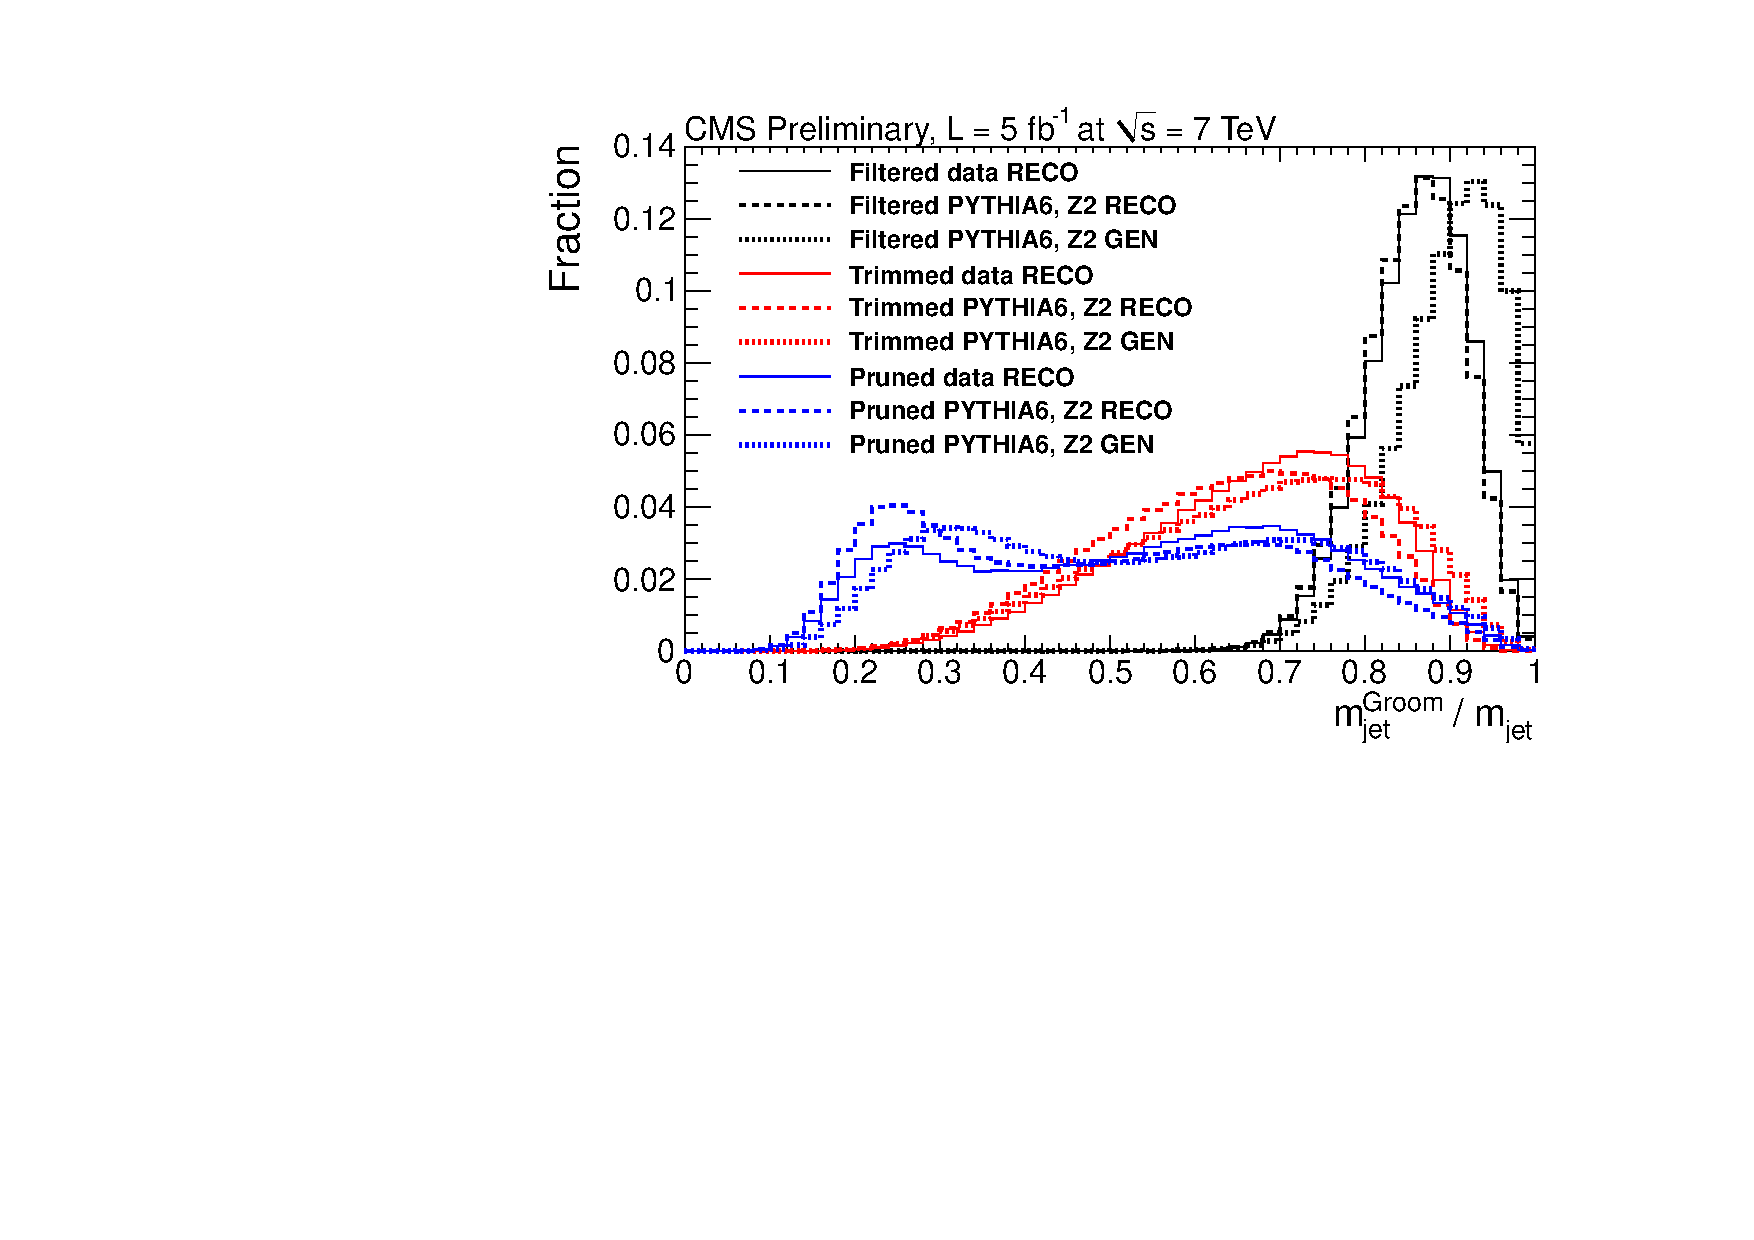
\includegraphics[width=0.95\textwidth]{figs/histAK7PtAvgVsMjetGroomOverReco_ratioPlots}
\caption{Comparison of the jet mass from the groomed jets
divided by the jet mass of matched ungroomed jets for the
three grooming techniques, for both data and the \PYTHIA Monte Carlo. 
\label{figs:histAK7PtAvgVsMjetGroomOverReco_ratioPlots}}
\end{figure}


\begin{figure}[htbp]
\centering
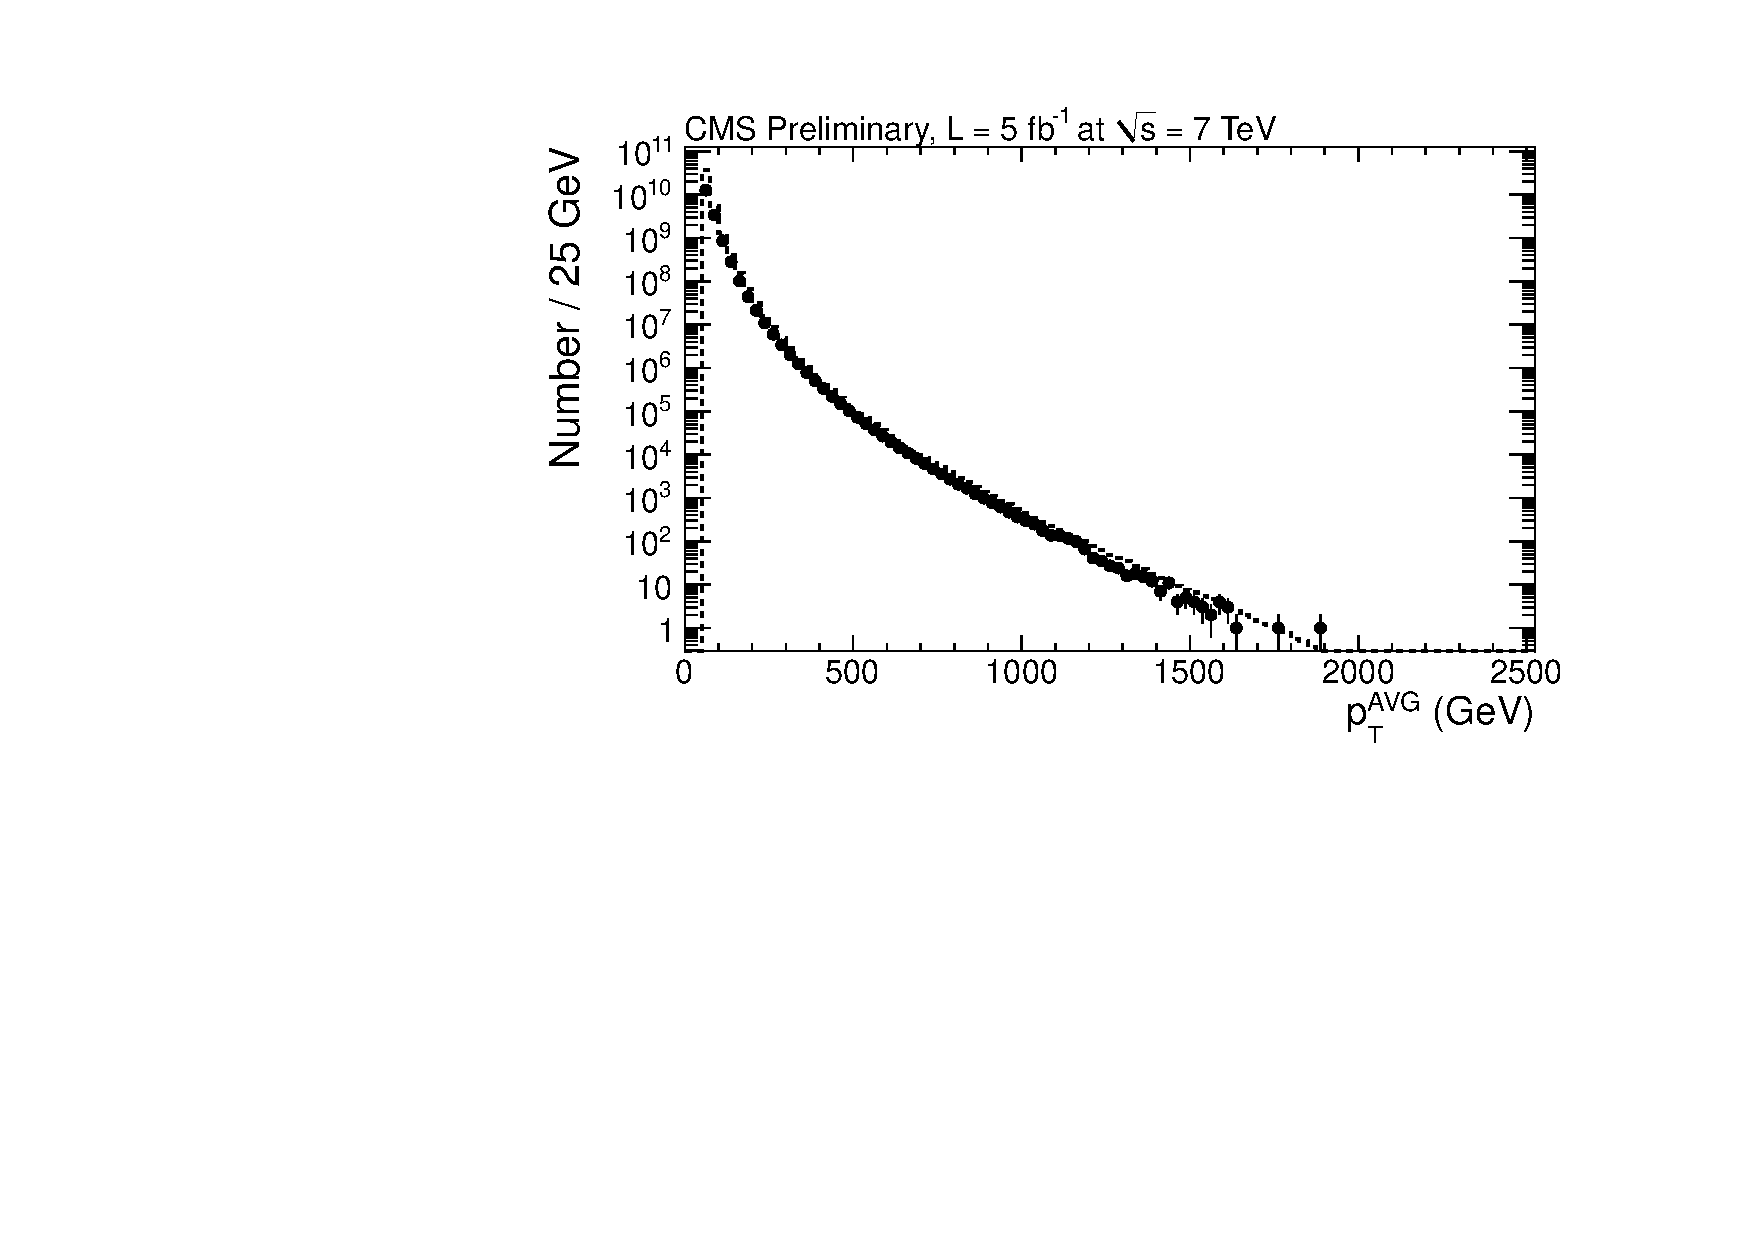
\includegraphics[width=0.95\textwidth]{figs/controlPlots_histAK7PtAvgVsNvtx}
\caption{Comparison of the $\pt^{AVG}$ distribution in data and
  \PYTHIA MC. 
\label{figs:controlPlots_histAK7PtAvgVsNvtx}}
\end{figure}



\begin{figure}[htbp]
\centering
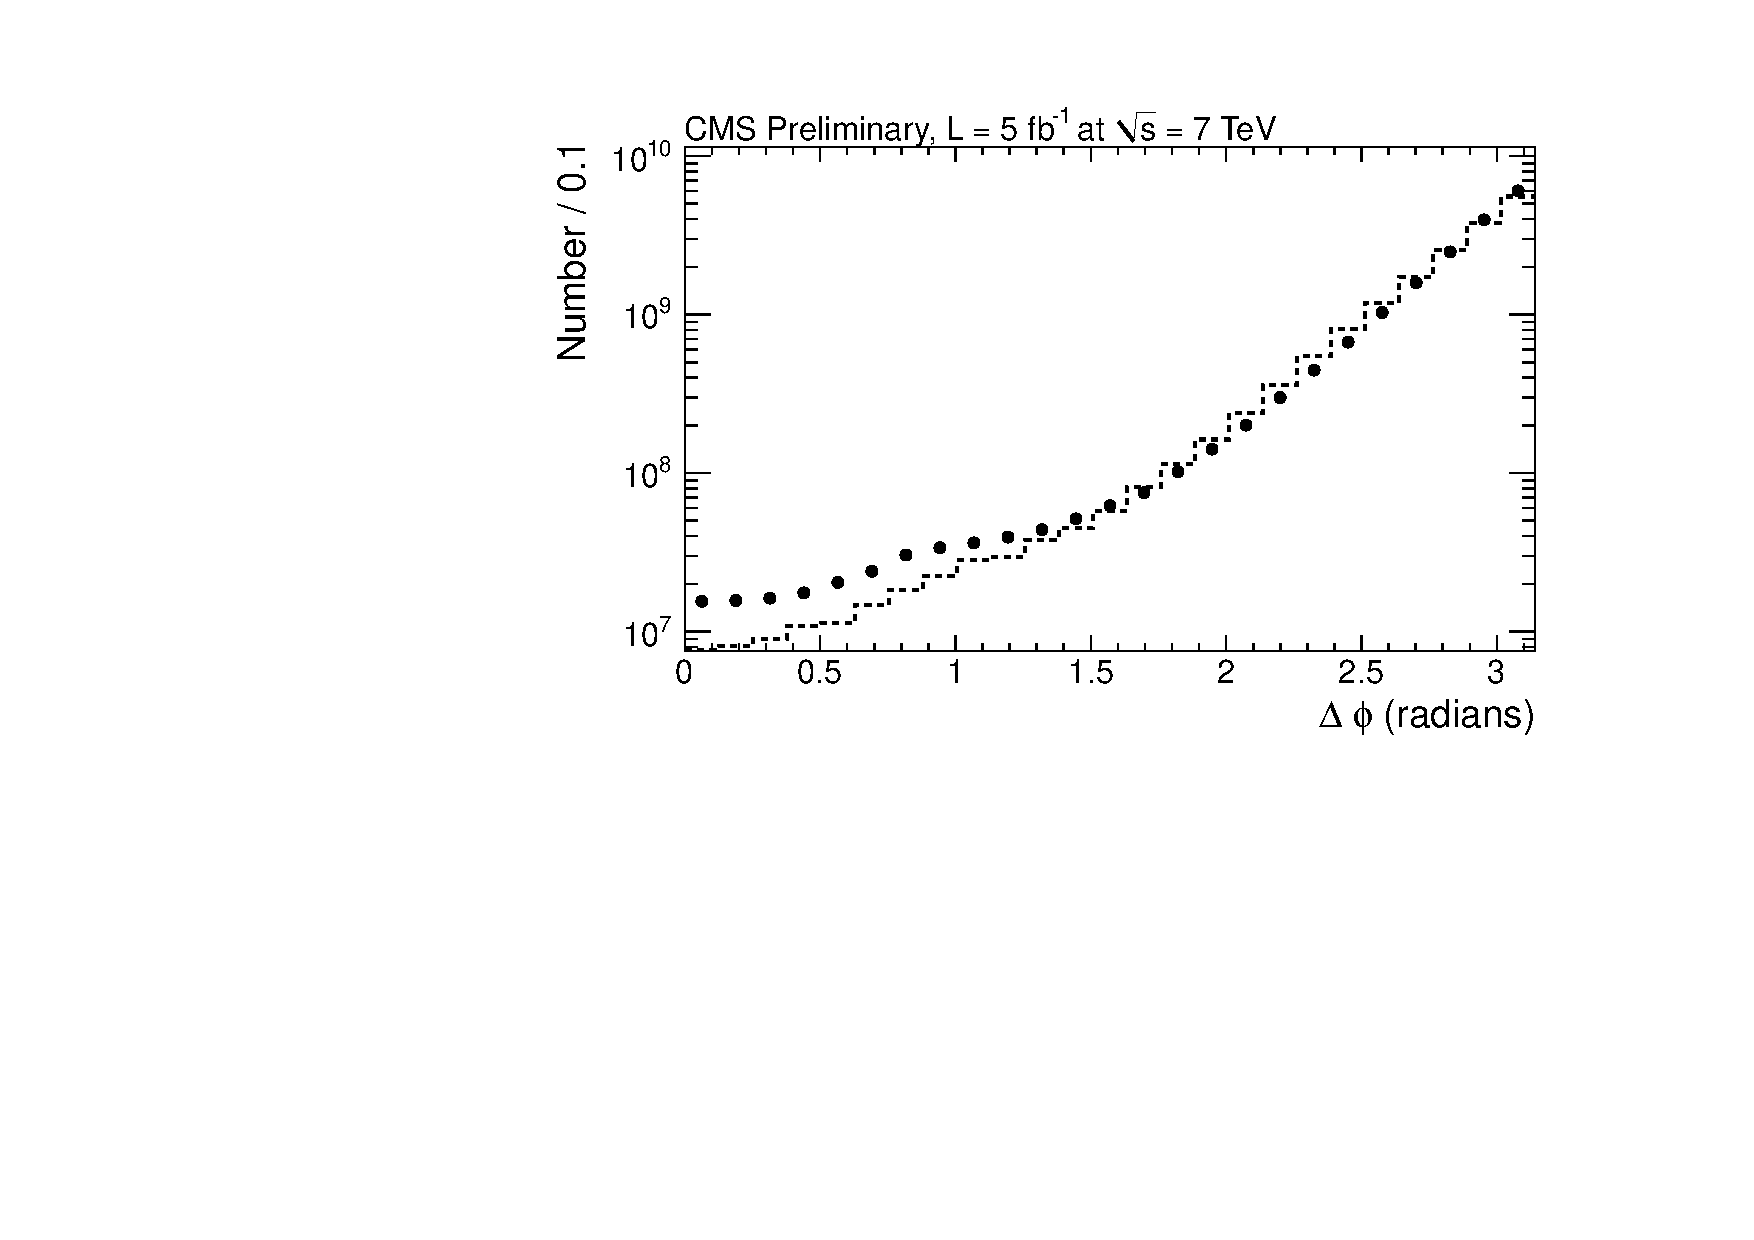
\includegraphics[width=0.95\textwidth]{figs/controlPlots_histAK7DeltaPhi}
\caption{Comparison of the $\Delta \phi$ distribution in data and
  \PYTHIA MC. 
\label{figs:controlPlots_histAK7DeltaPhi}}
\end{figure}



\clearpage

\section{Unfolding procedure}
The unfolding procedure is exactly the same as in Ref.~\cite{cmsSMPJSVJ}. Here we discuss the unfolding
briefly for completeness. 

\subsection{Unfolding}
The measured spectrum of a physical observable, like the jet mass distribution, is usually distorted by	detector effects, such as finite resolution and limited acceptance. Moreover, in this analysis the chosen bin size is comparabl
e to the resolution, so there is a significant migration of events generated in one jet bin mass and ending up in a different bin of reconstructed jet mass. A comparison of the measured mass spectrum with that predicted at generato
r level requires that we remove these effects to obtain the true underlying mass spectrum. There are several possible ways to achieve the unfolding of detector effects on measured spectra, and examples can be found in \cite{unfold}
 and references therein. In this section we describe the unfolding method adopted in this analysis, which largely follows the technique proposed in \cite{agostini}. 
A physical quantity $\alpha$, distributed according to its probability density function $f(\alpha)$, cannot be measured perfectly. Apart from statistical uncertainties, there will be effects from reconstruction efficiency and finite 
resolution of the detector. As	a result, instead of the true, physical variable $\alpha$, 
a variable $\beta$, distributed according to some distribution $g(\beta)$, is measured. 
The relation between $f(\alpha)$ and $g(\beta)$ can be expressed as a convolution of the 
true distribution $f(\alpha)$ with a kernel $\hat{A}(\alpha,\beta)$ describing the detector effects,

\begin{equation}
\int f(\alpha) \hat{A}(\alpha,\beta)d\alpha = g(\beta)
\end{equation}

\noindent The spectrum we intend to unfold is given as an histogram. Hence, we use vectors and matrices for the formulation of the convolution,	

\begin{equation}
\hat{A} x = b
\label{eq:unf1}
\end{equation}

\noindent where the $i$-th component of the $n_x$-dimensional vector $x$ and the $n_b$-dimensional vector $b$ contain the number of entries in bin $i$ of the true and the measured distribution, respectively. 
$\hat{A}$ is a $(n_b - n_x)$-dimensional matrix, and contains the detector effects. An event with a true value in bin $j$ might be measured with a value in bin $i$ (i.e. finite resolution) or might not be measured at all. The matri
x element $\hat{A}_{ij}$ represents the probability for an event	 with a true value in bin $x_j$ to be measured with a value in bin $b_i$.
Assuming that the measurement process is well simulated, $\hat{A}$ can be determined on Monte Carlo events by tracking the true and reconstructed values for each event. A well-defined system of linear equations is obtained,

\begin{equation}
\hat{A} x^{ini} = b^{ini}
\end{equation}


\noindent where the index ``ini''denotes the use of Monte Carlo spectra $x^{ini}$ , $b^{ini}$. Technically, the matrix element $\hat{A}_{ij}$ is determined by taking the number of events that fall into bin $j$ of $x^{ini}$ and at t
he same time into bin $i$ of $b^{ini}$, and by dividing this number by the number of events in bin $j$ of $x^{ini}$.

Now that $\hat{A}$ is determined and we have a measured spectrum $b$, one can try to solve Eq.~\ref{eq:unf1} for the true spectrum $x$. However, the apparently easiest way to determine $x$, i.e. applying $x = \hat{A}^{-1}b$, is not
 adequate. Even when $\hat{A}$ can be inverted, statistical fluctuations in the measured spectrum introduce spurious, non-physical oscillations in the solution for $x$. Therefore a more efficient method needs to be applied. 

We use an unfolding procedure described by G.~D.~Agostini in~\cite{agostini}. Repeated application of Bayes theorem is used to invert the response matrix. Regularization is achieved by stopping iterations before reaching the ``true
'' (but wildly fluctuating) inverse. The regularization parameter is just the number of iterations.
 In principle, this has to be tuned to prevent the statistical fluctuations being interpreted as structure in the true distribution, according to the sample statistics and binning. In practice, the results are fairly insensitive to
 the precise setting used and four iterations are usually sufficient.
The training truth is taken as its initial prior, rather than a flat distribution. This should not bias result once we have iterated, but could reach an optimum after fewer iterations.
This implementation takes account of errors on the data sample but not, by default, uncertainties in the response matrix due to finite MC statistics. That calculation can be very slow, and usually the training sample is much larger
 than the data sample.
%RooUnfoldBayes does not normally do smoothing, since this has not been found to be necessary 2
%and can, in principle, bias the distribution. Smoothing can be enabled with an option.

\ifnpas
The {\tt RooUnfold} package~\cite{roounfold} has been used with the {\tt RooUnfoldBayes} class,
with the number of iterations set to four. 
\fi

\subsection{Response matrices}

The detector response matrix for the different jet clustering algorithms are showed in Fig.~\ref{figs:response_QCD_pythia6_z2_plots_nominal_ptall}-\ref{figs:response_QCD_herwigpp_23_plots_nominal_Pruned_ptall}. 
We show the response in the nine nominal $p_T$ bins used for the analysis, for the AK7 jets with the 
following clustering algorithm: ungroomed, pruned, filtered and trimmed.
In the response matrix derivation, the appropriate physical $\pt$ weighting is
used. If one uses the unphysical flat-$\pt$ spectrum, this introduces
unphysical biases in the tails of the jet mass distribution. 



\begin{figure}[htbp]
\centering
\subfigure{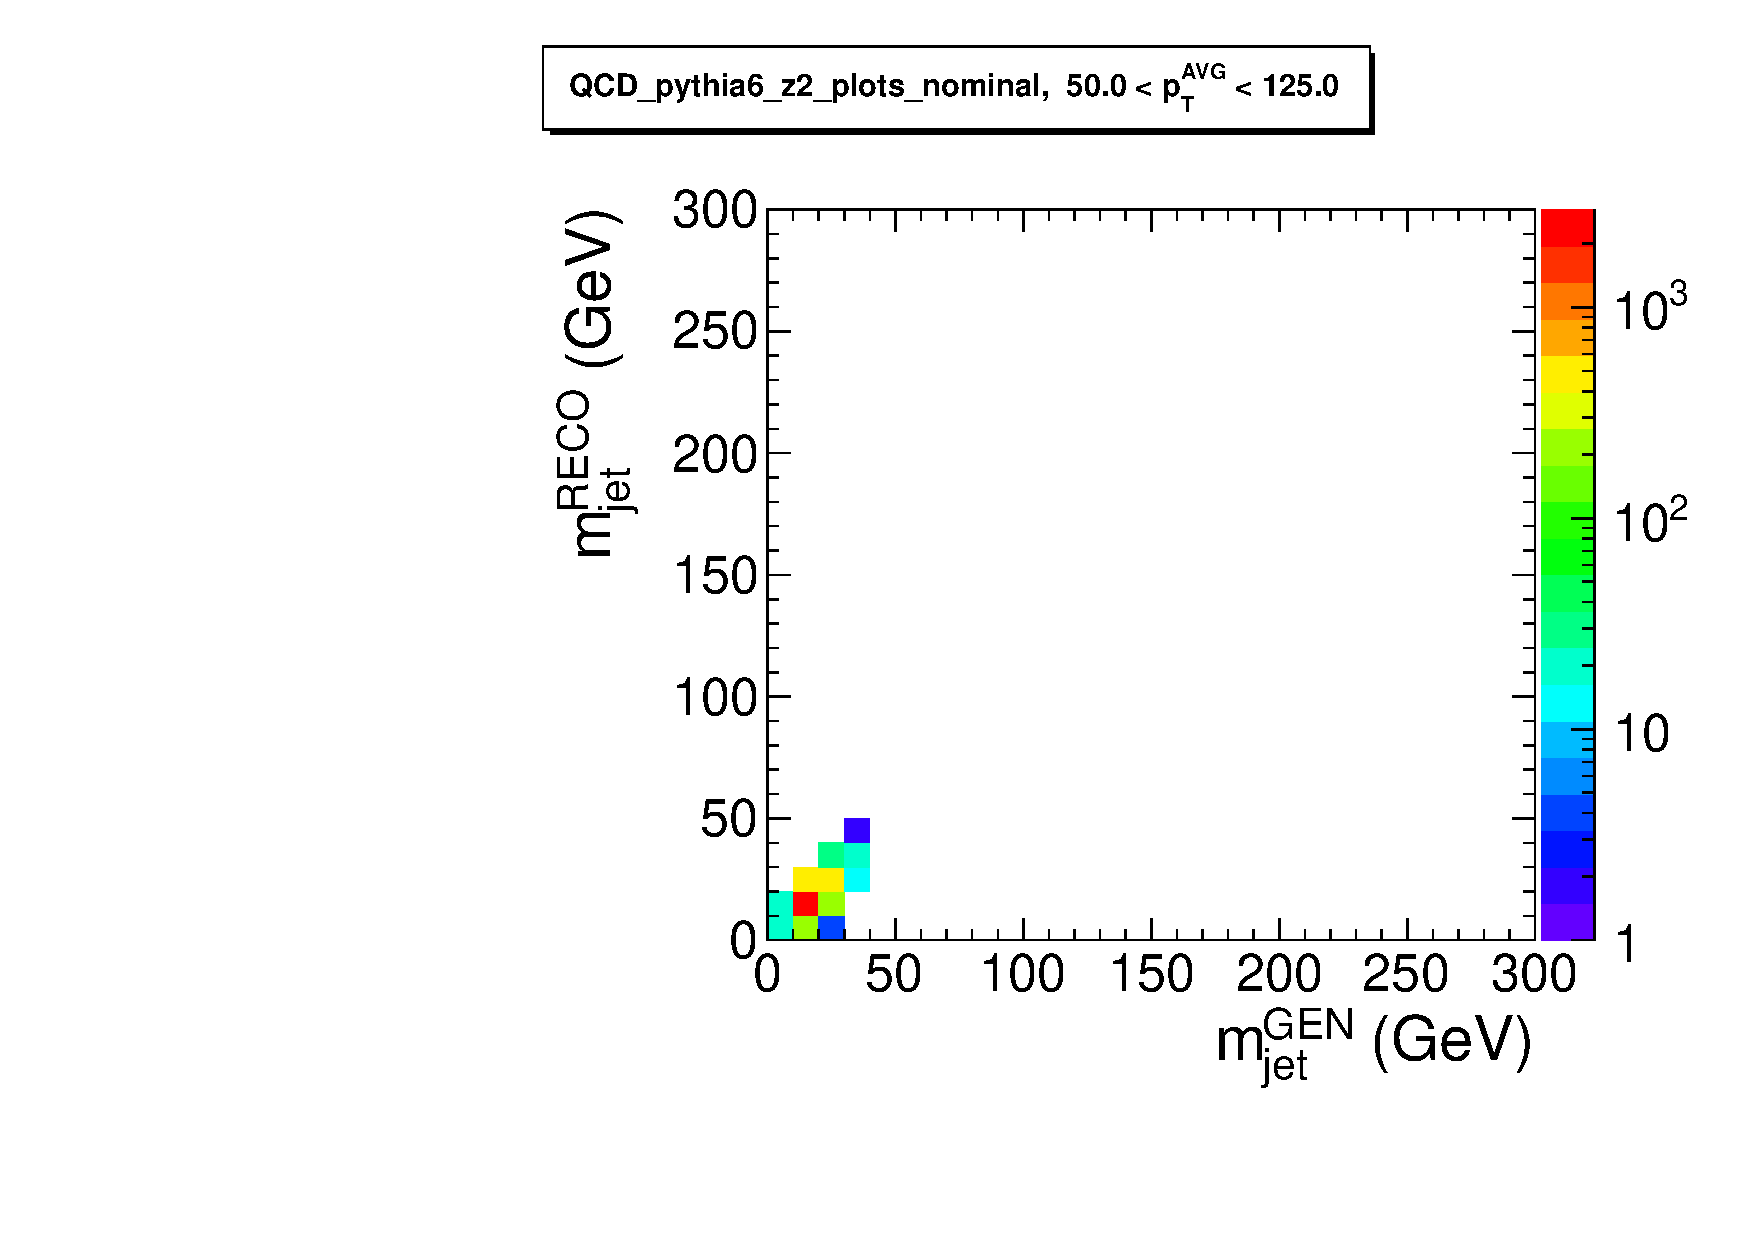
\includegraphics[width=0.3\textwidth]{figs/response_QCD_pythia6_z2_plots_nominal_pt1}}
\subfigure{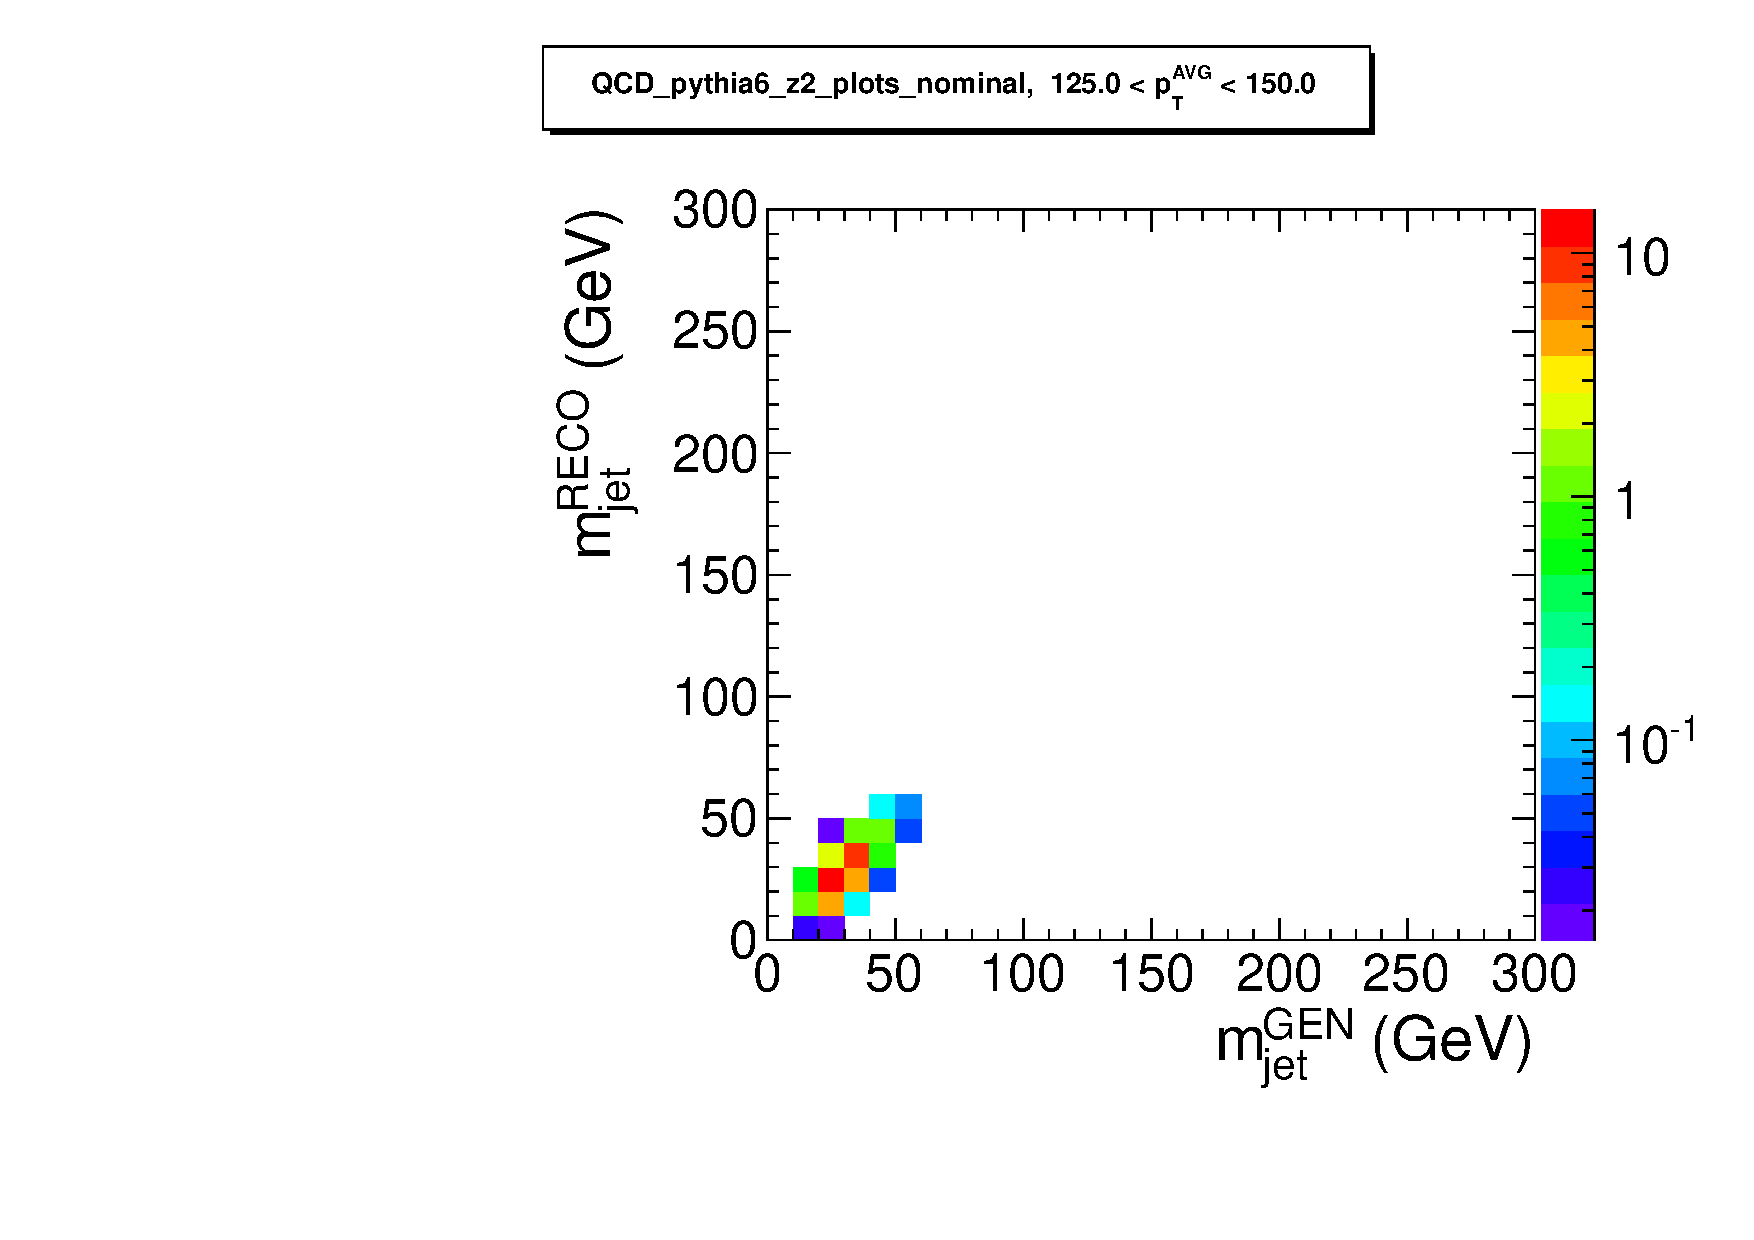
\includegraphics[width=0.3\textwidth]{figs/response_QCD_pythia6_z2_plots_nominal_pt2}}
\subfigure{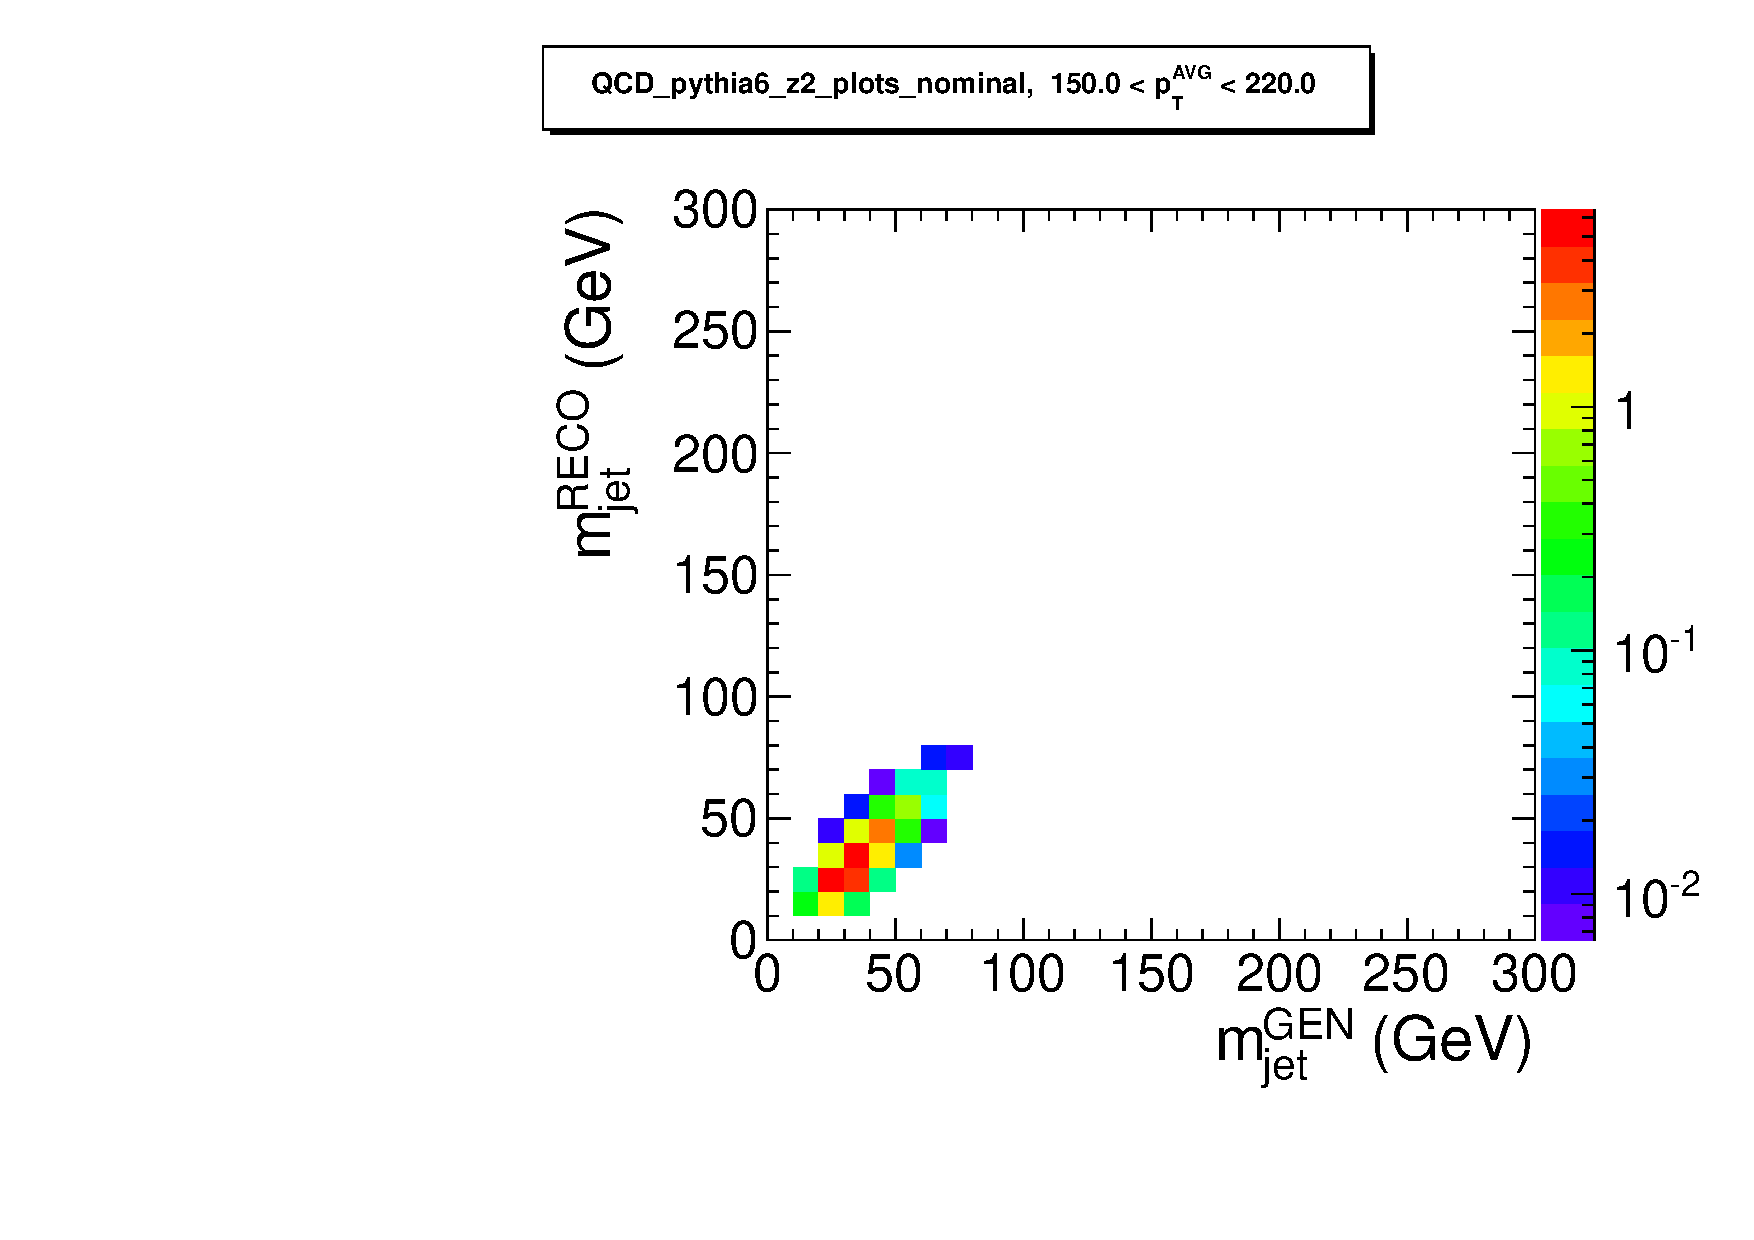
\includegraphics[width=0.3\textwidth]{figs/response_QCD_pythia6_z2_plots_nominal_pt3}}\\
\subfigure{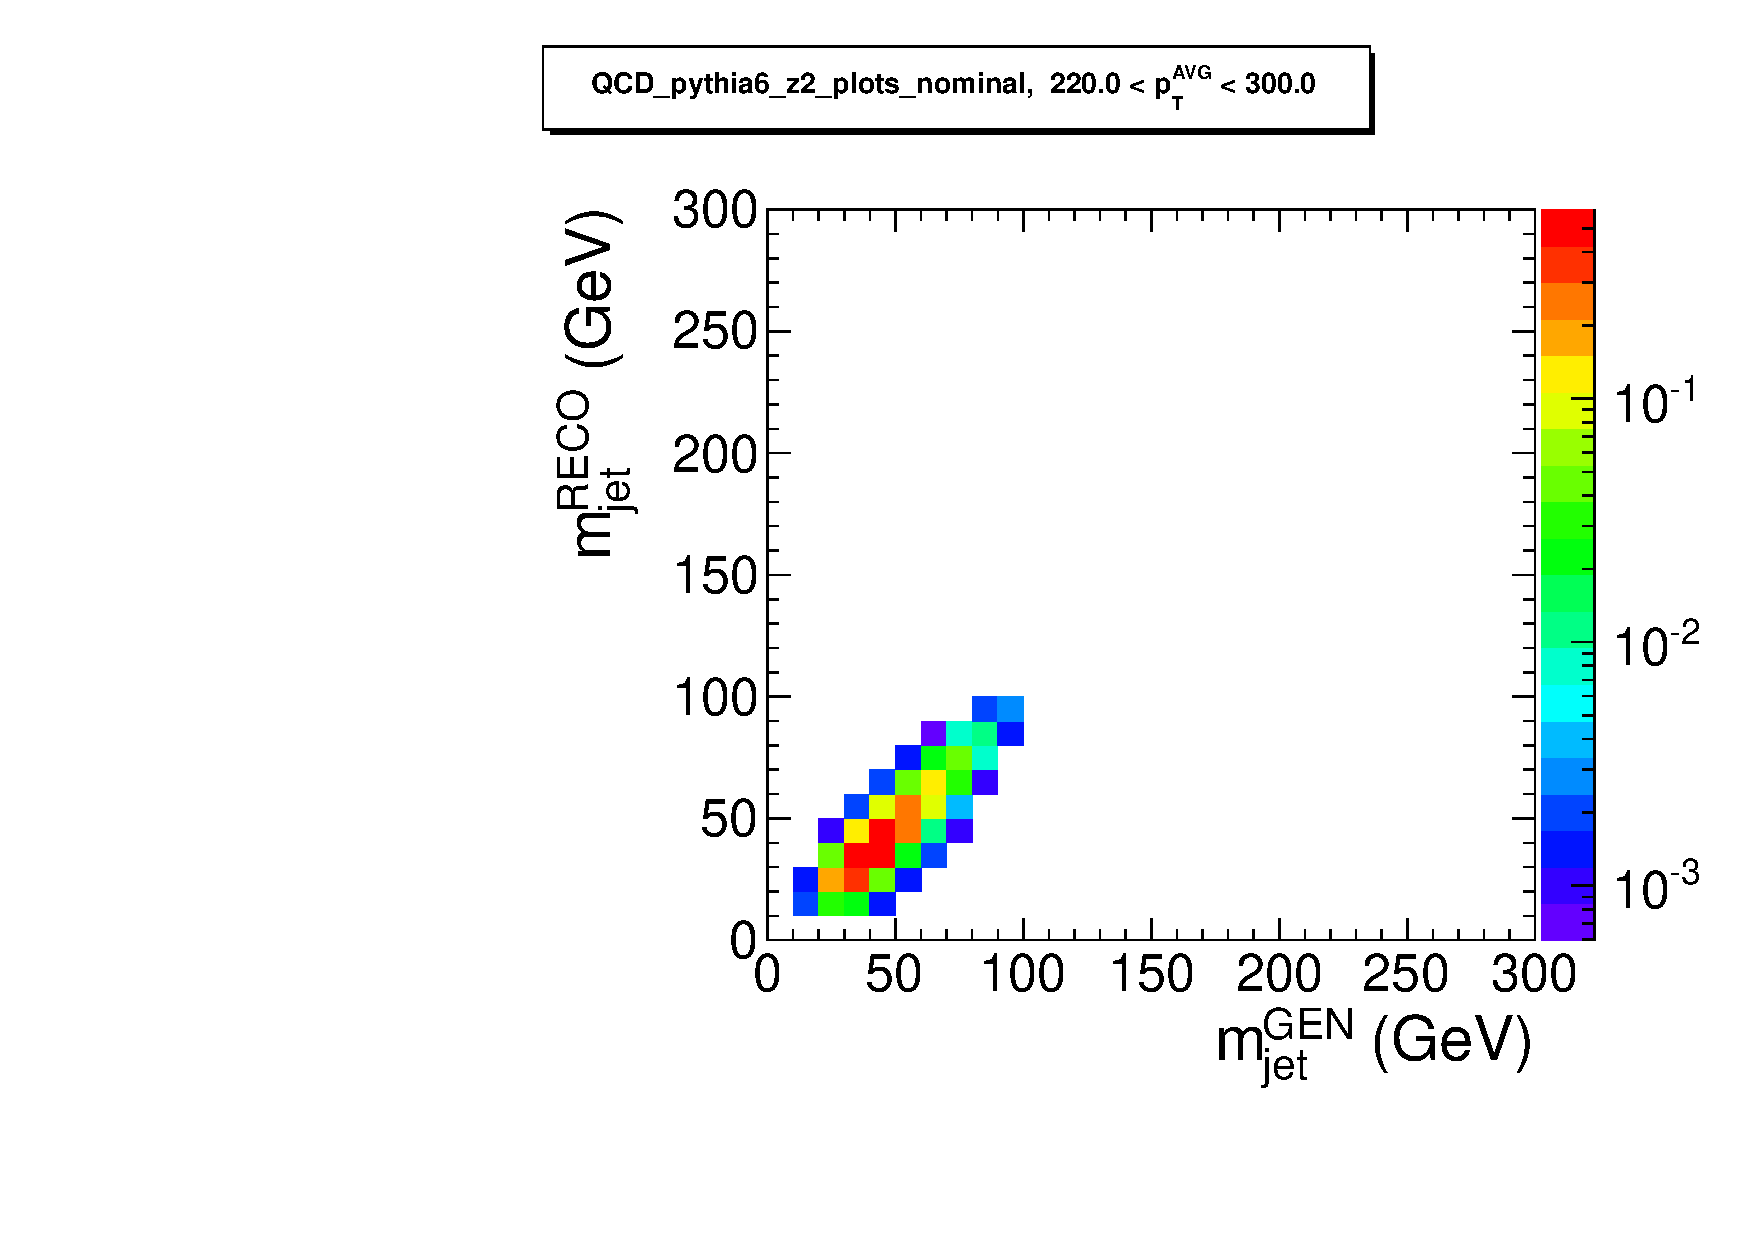
\includegraphics[width=0.3\textwidth]{figs/response_QCD_pythia6_z2_plots_nominal_pt4}}
\subfigure{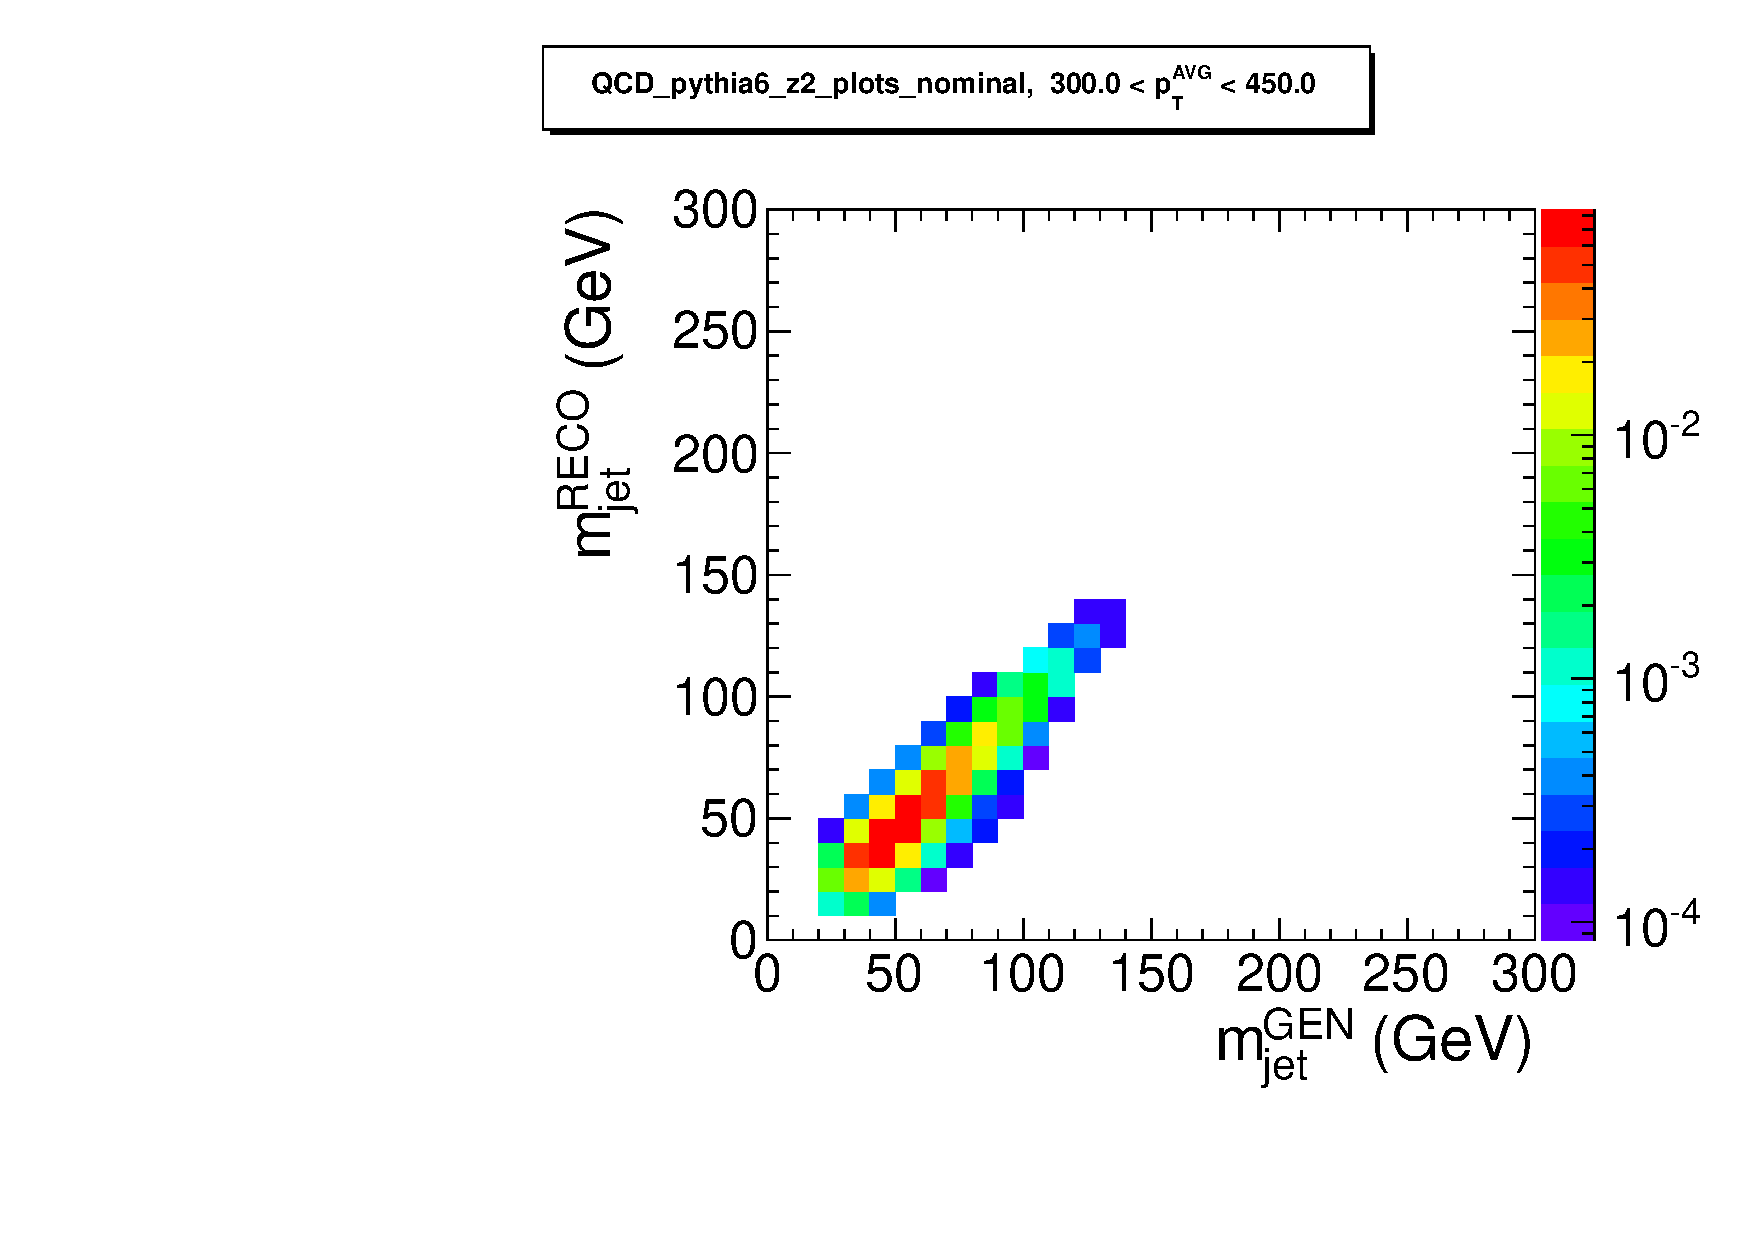
\includegraphics[width=0.3\textwidth]{figs/response_QCD_pythia6_z2_plots_nominal_pt5}}
\subfigure{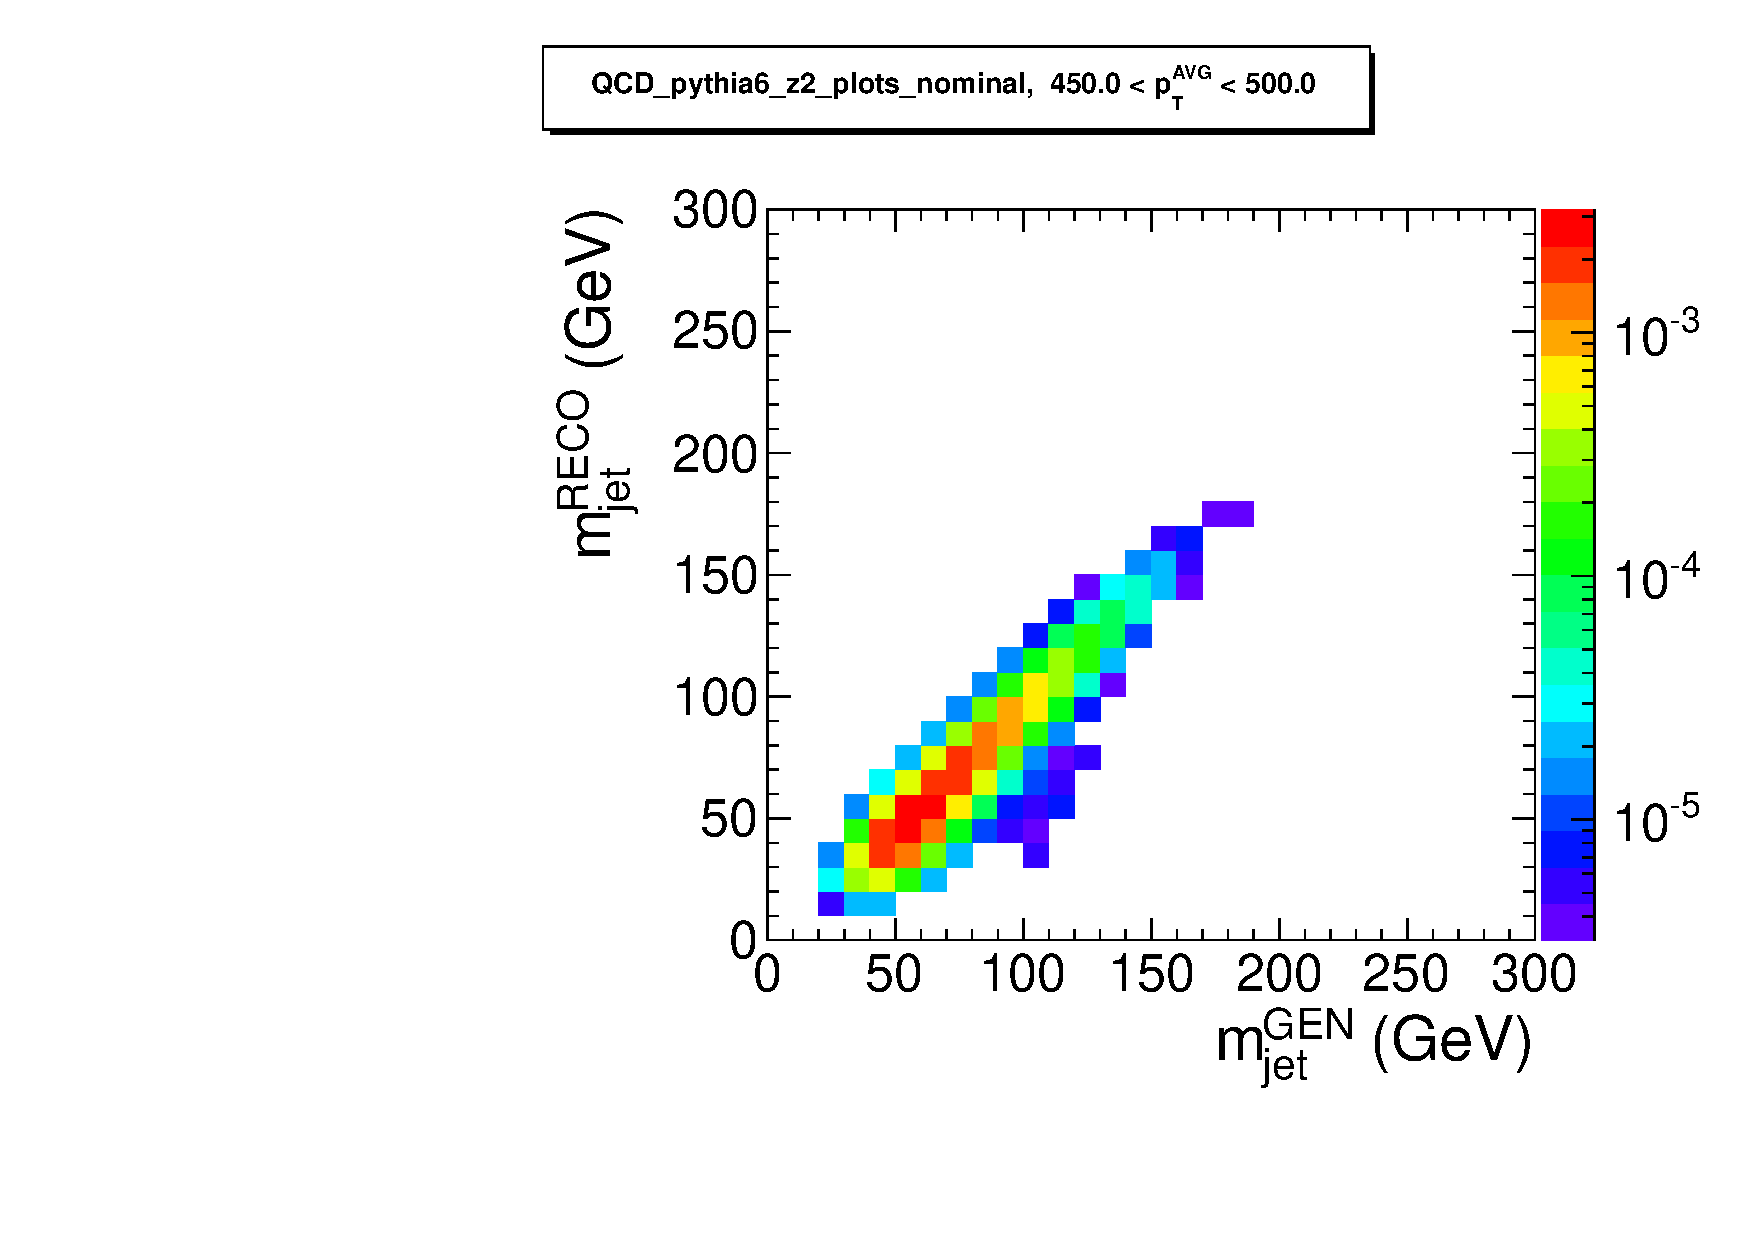
\includegraphics[width=0.3\textwidth]{figs/response_QCD_pythia6_z2_plots_nominal_pt6}}\\
\subfigure{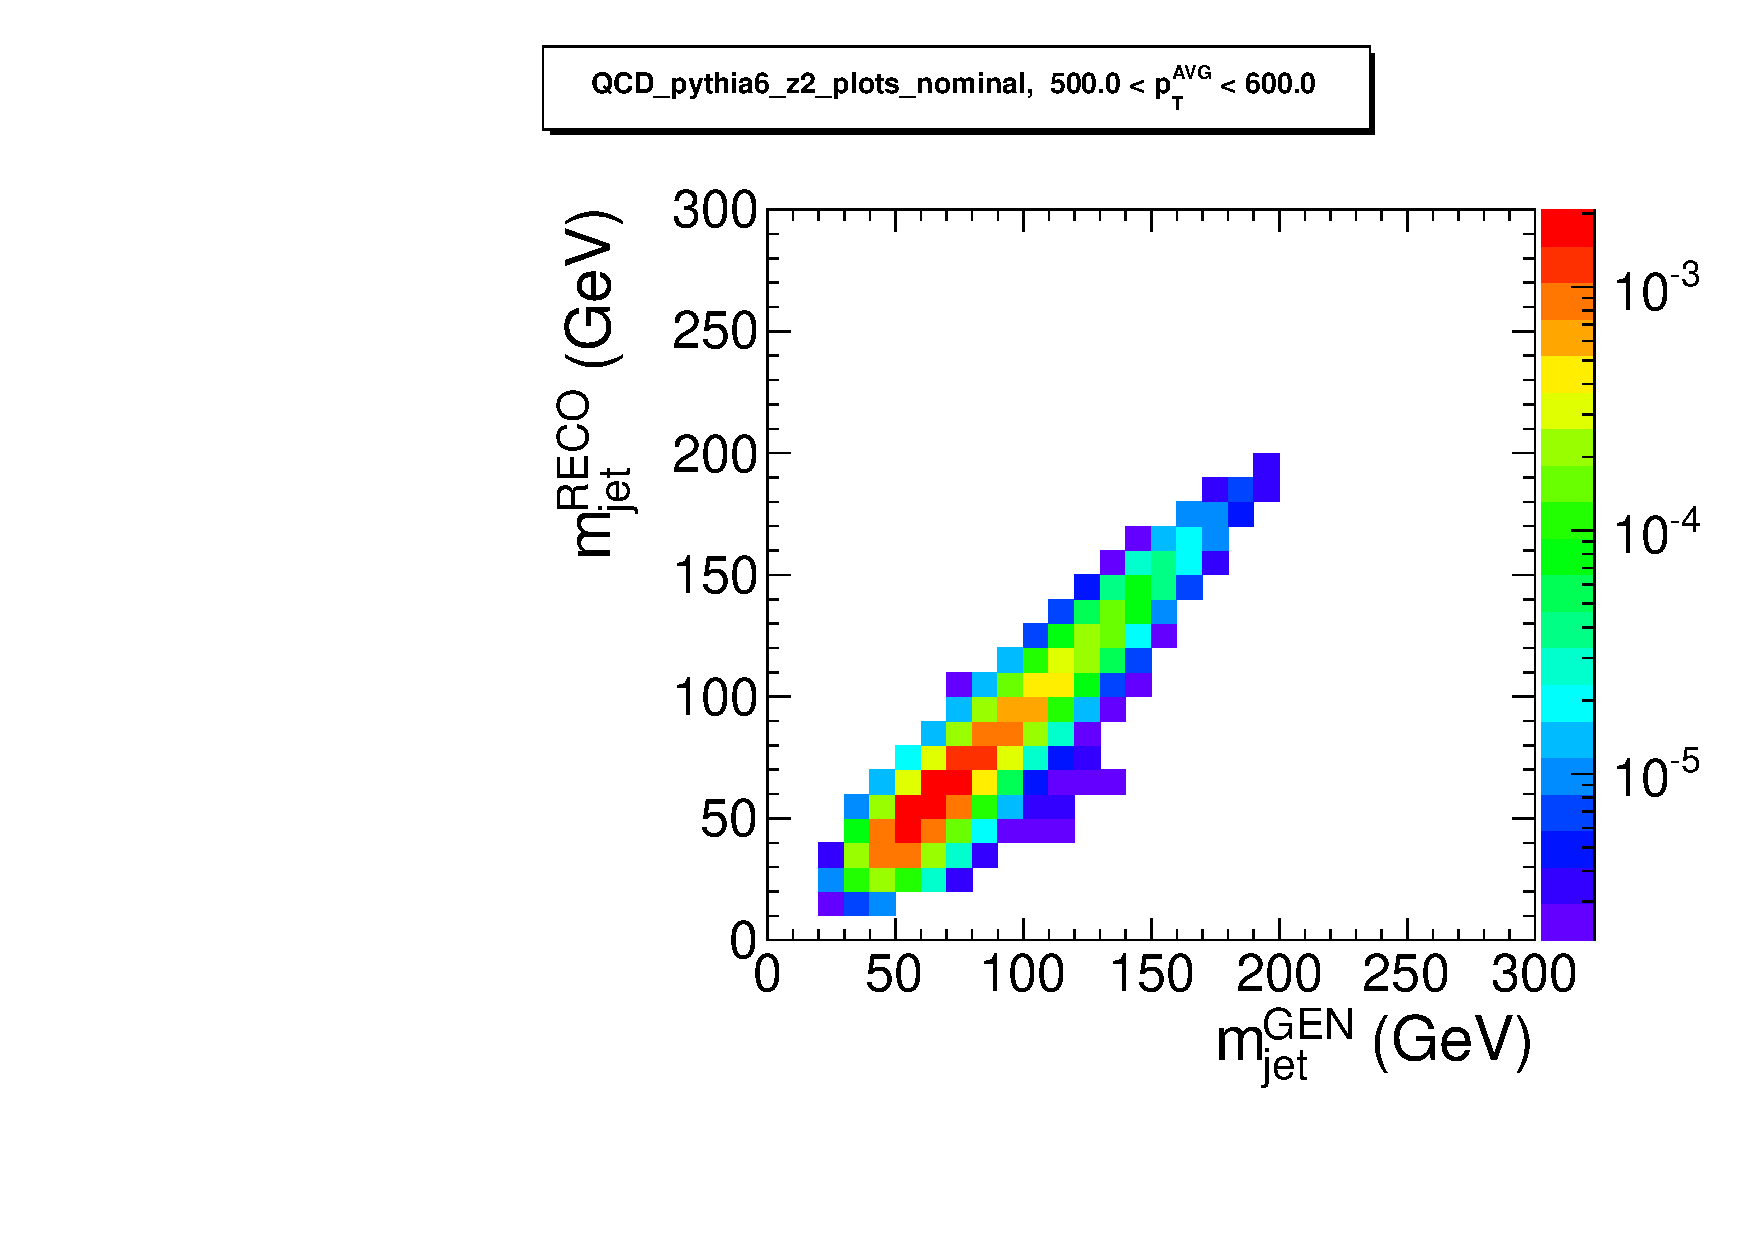
\includegraphics[width=0.3\textwidth]{figs/response_QCD_pythia6_z2_plots_nominal_pt7}}
\subfigure{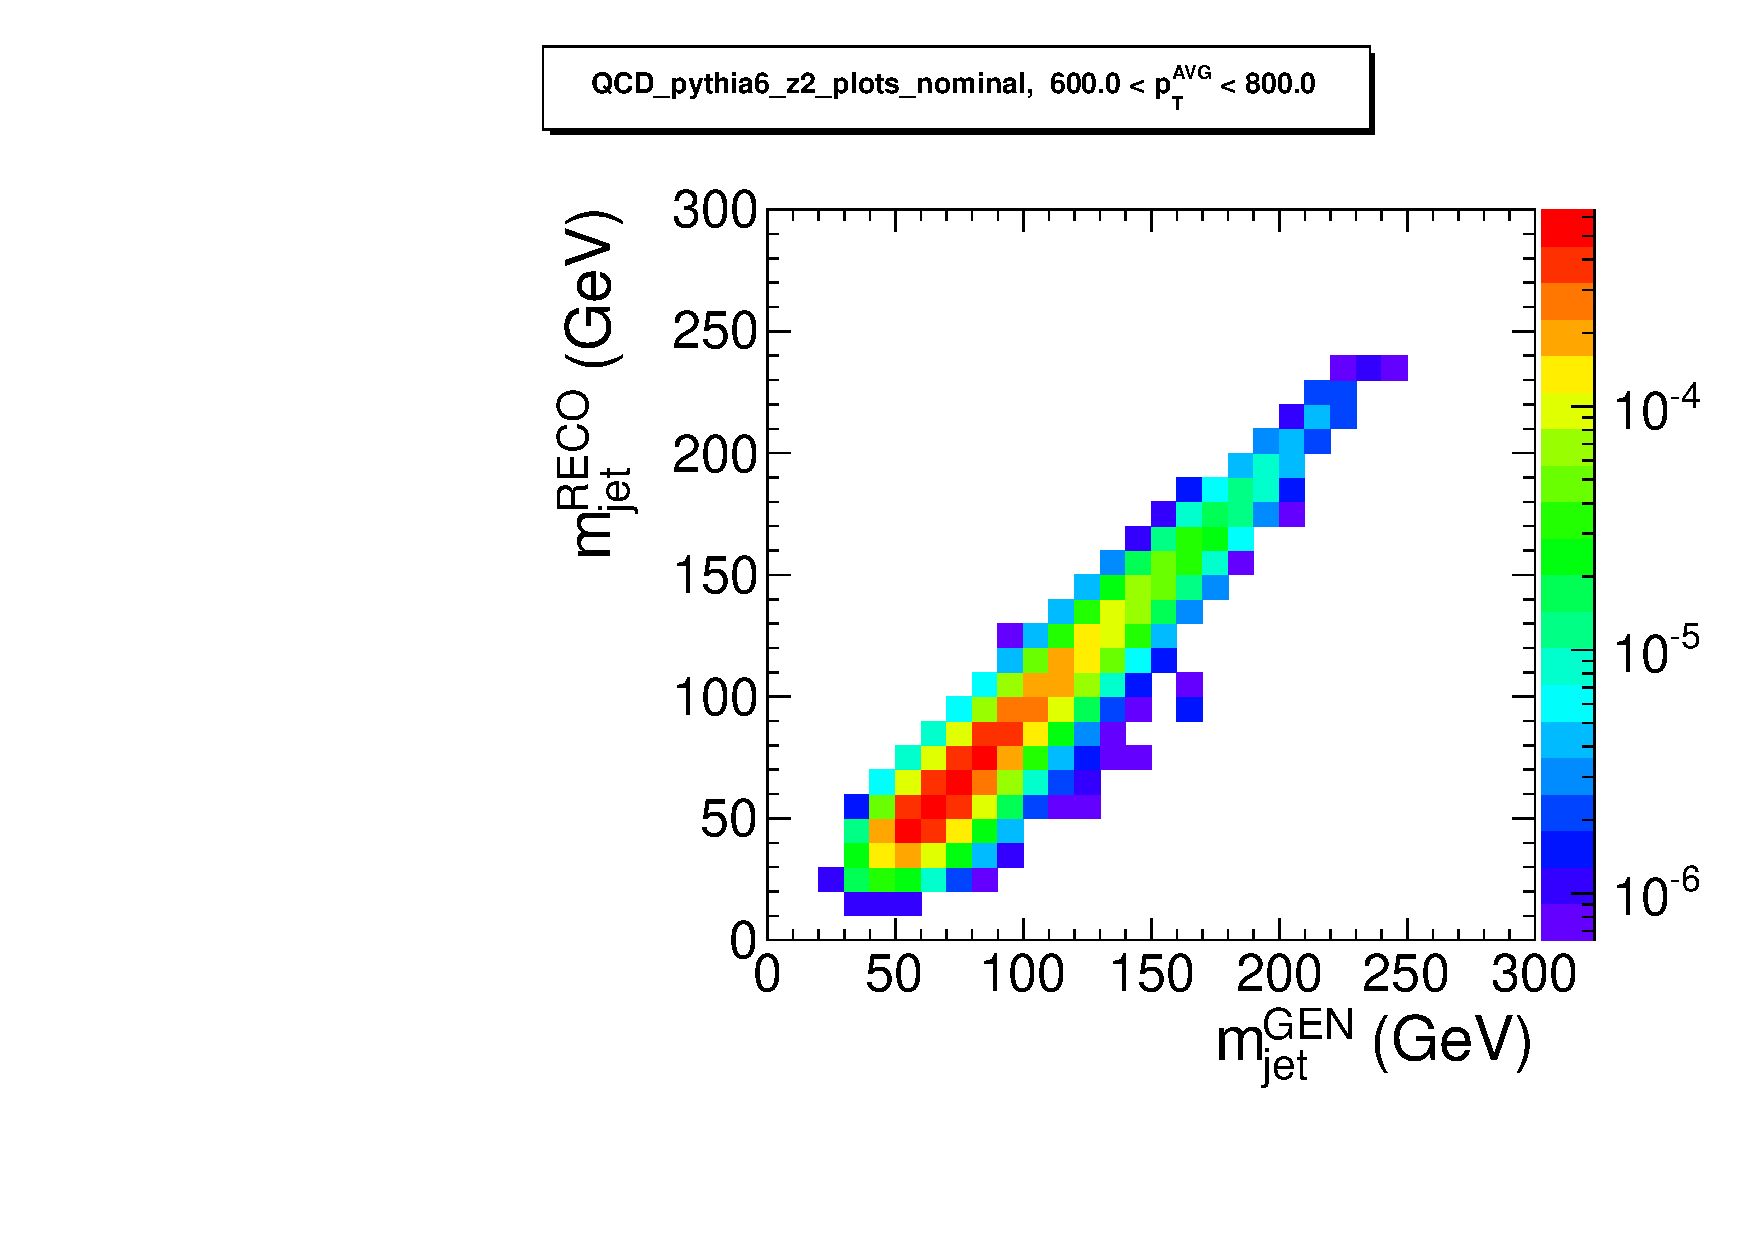
\includegraphics[width=0.3\textwidth]{figs/response_QCD_pythia6_z2_plots_nominal_pt8}}
\subfigure{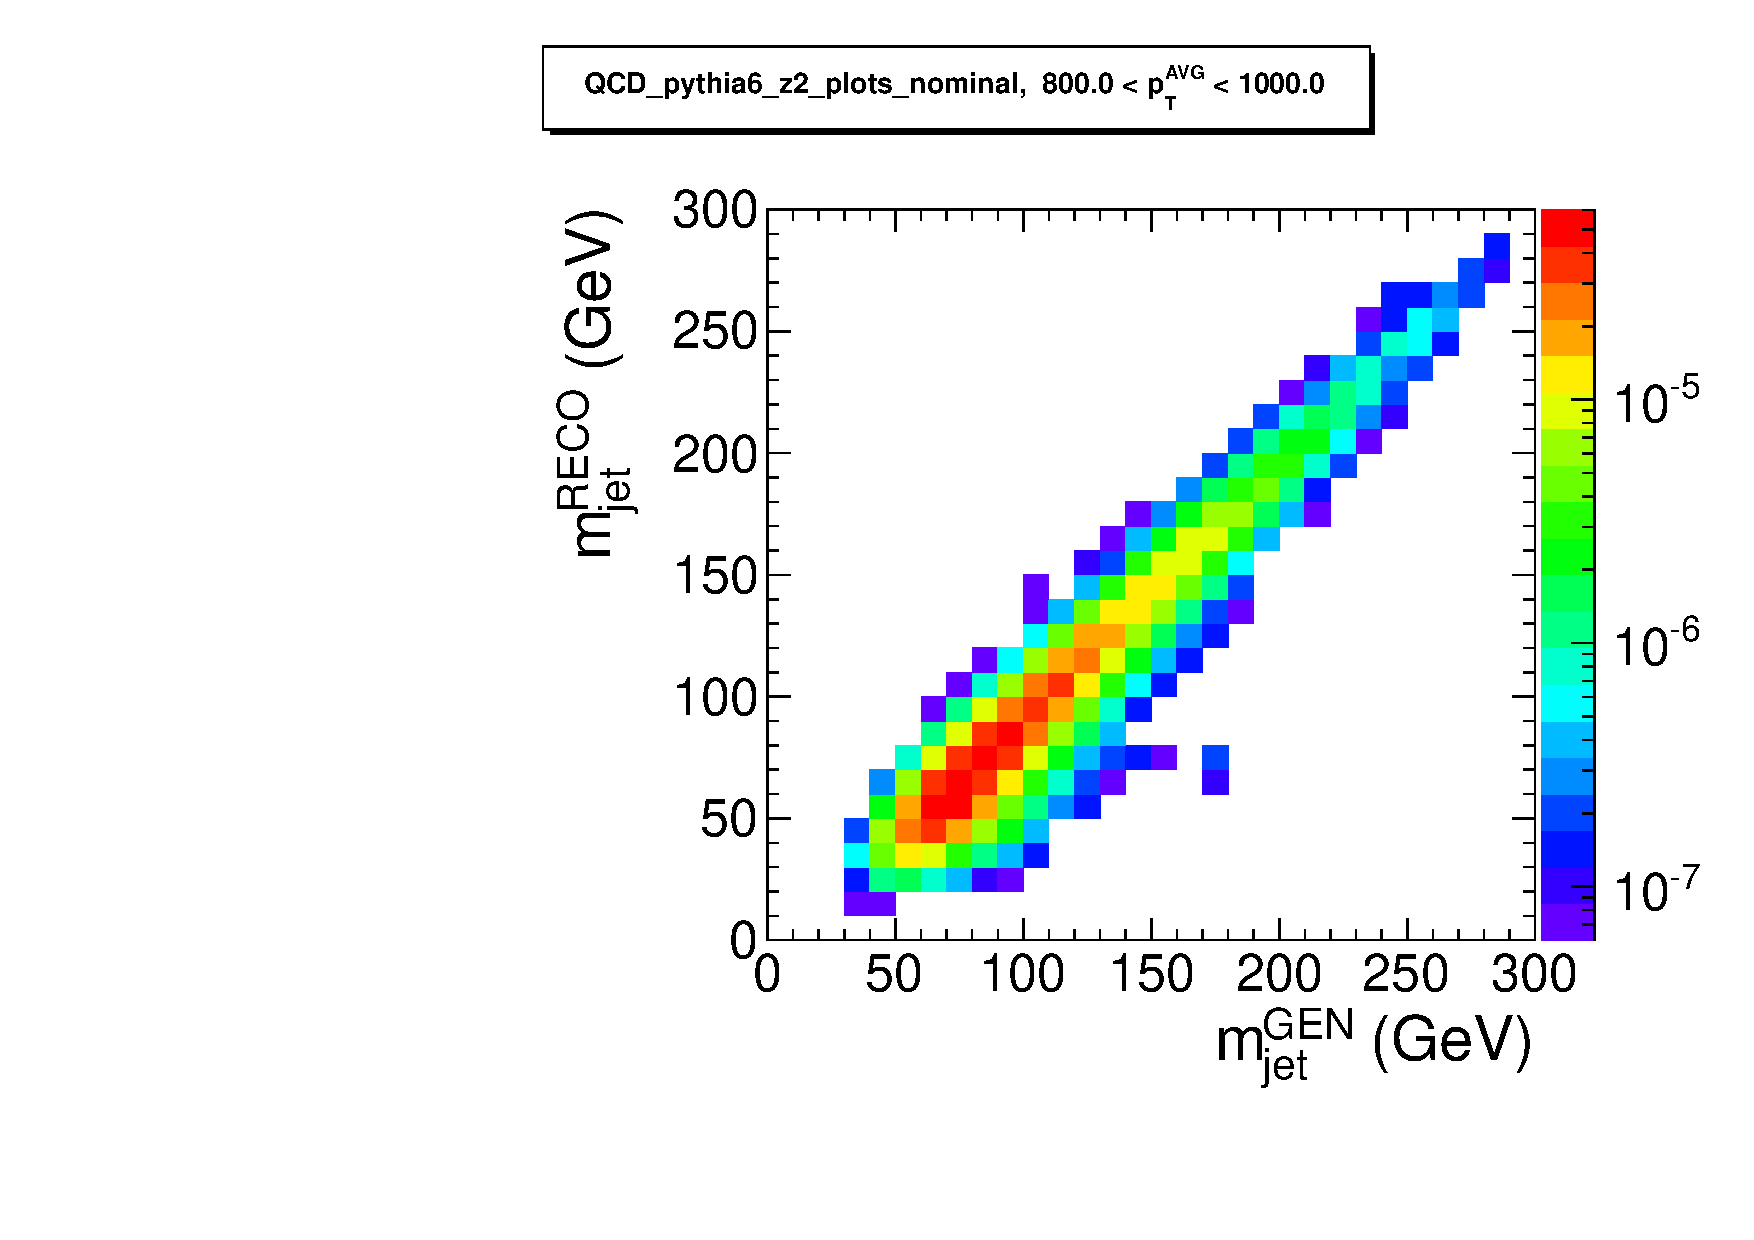
\includegraphics[width=0.3\textwidth]{figs/response_QCD_pythia6_z2_plots_nominal_pt9}}\\
\caption{Response of the jet mass for AK7 jets,
for various $\pt^{AVG}$ bins. The true jet mass is shown
on the $x-$axis, and the reconstructed jet mass is shown on the
$y-$axis, using the \PYTHIA generator. 
\label{figs:response_QCD_pythia6_z2_plots_nominal_ptall}}
\end{figure}


\clearpage

\begin{figure}[htbp]
\centering
\subfigure{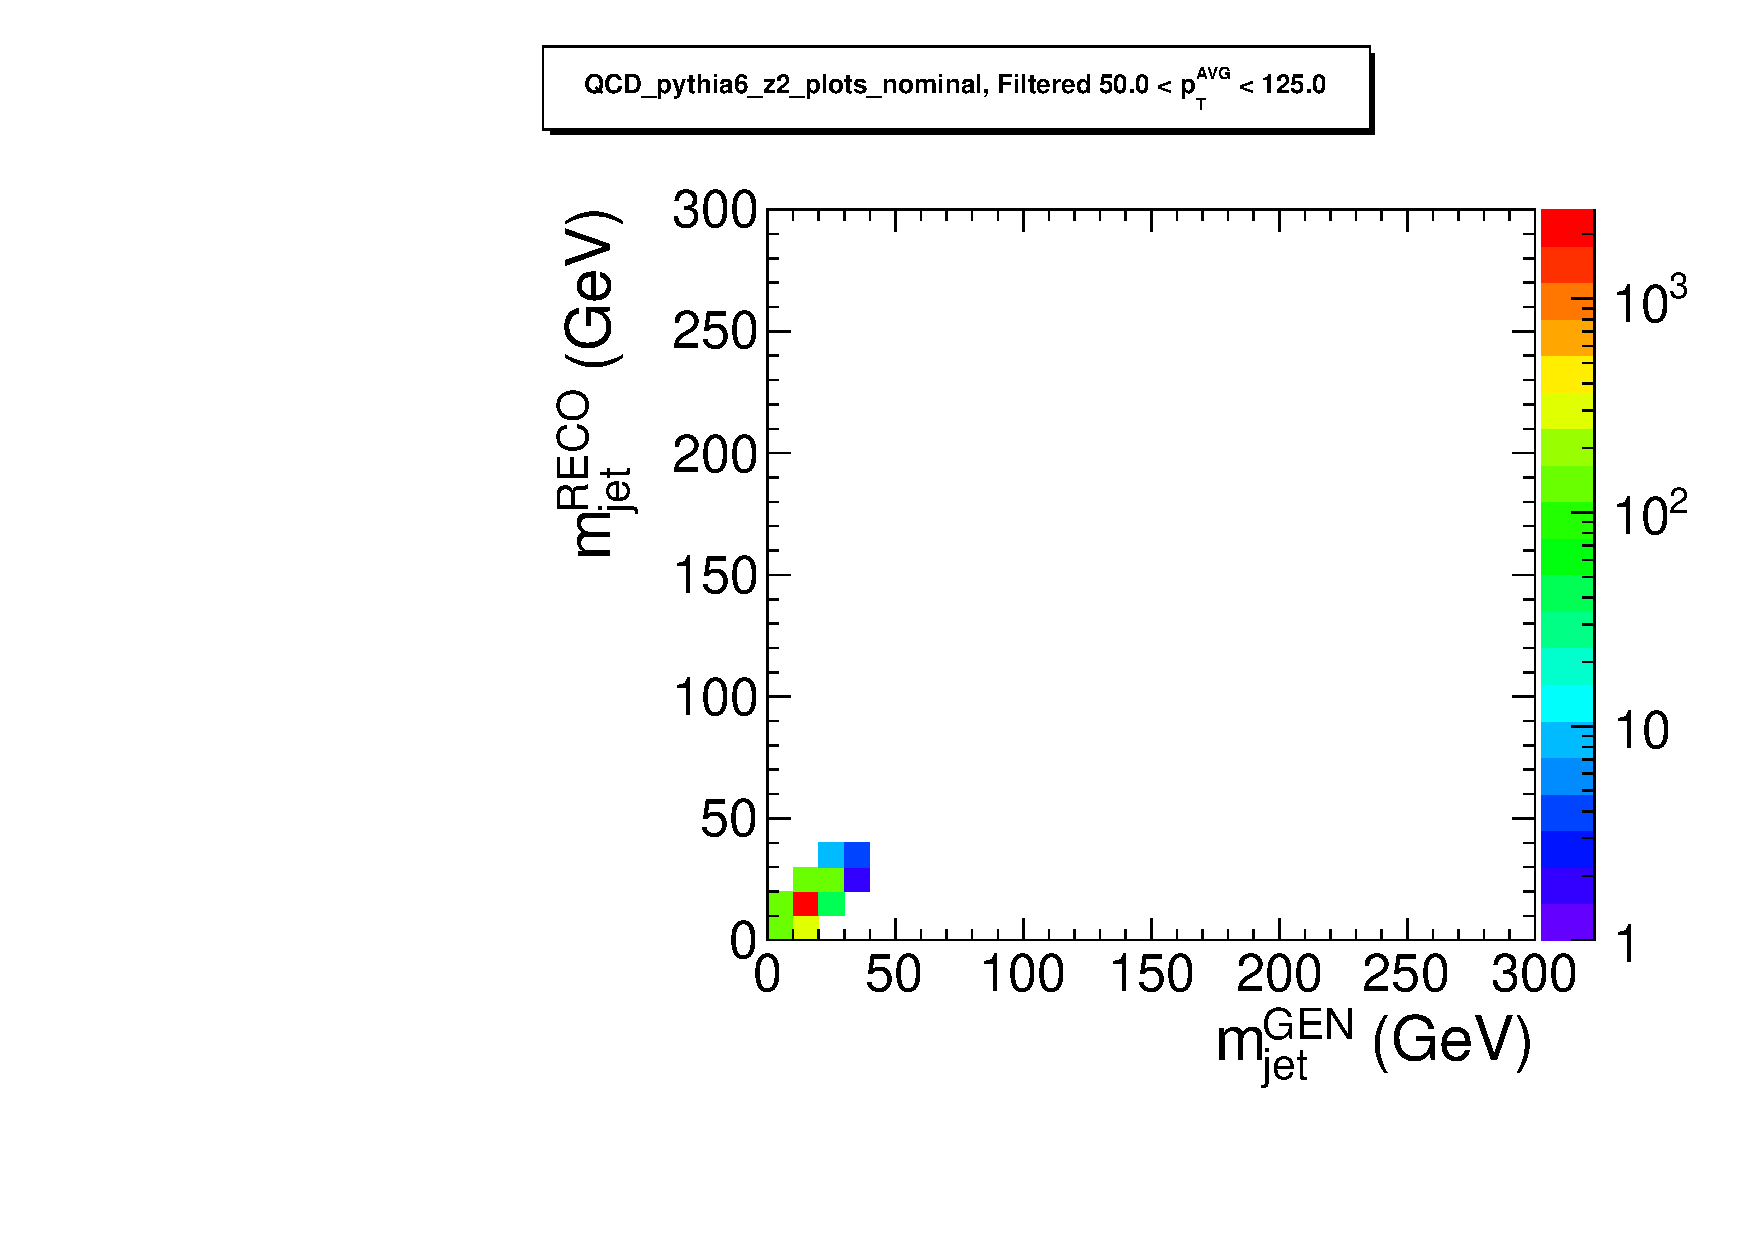
\includegraphics[width=0.3\textwidth]{figs/response_QCD_pythia6_z2_plots_nominal_Filtered_pt1}}
\subfigure{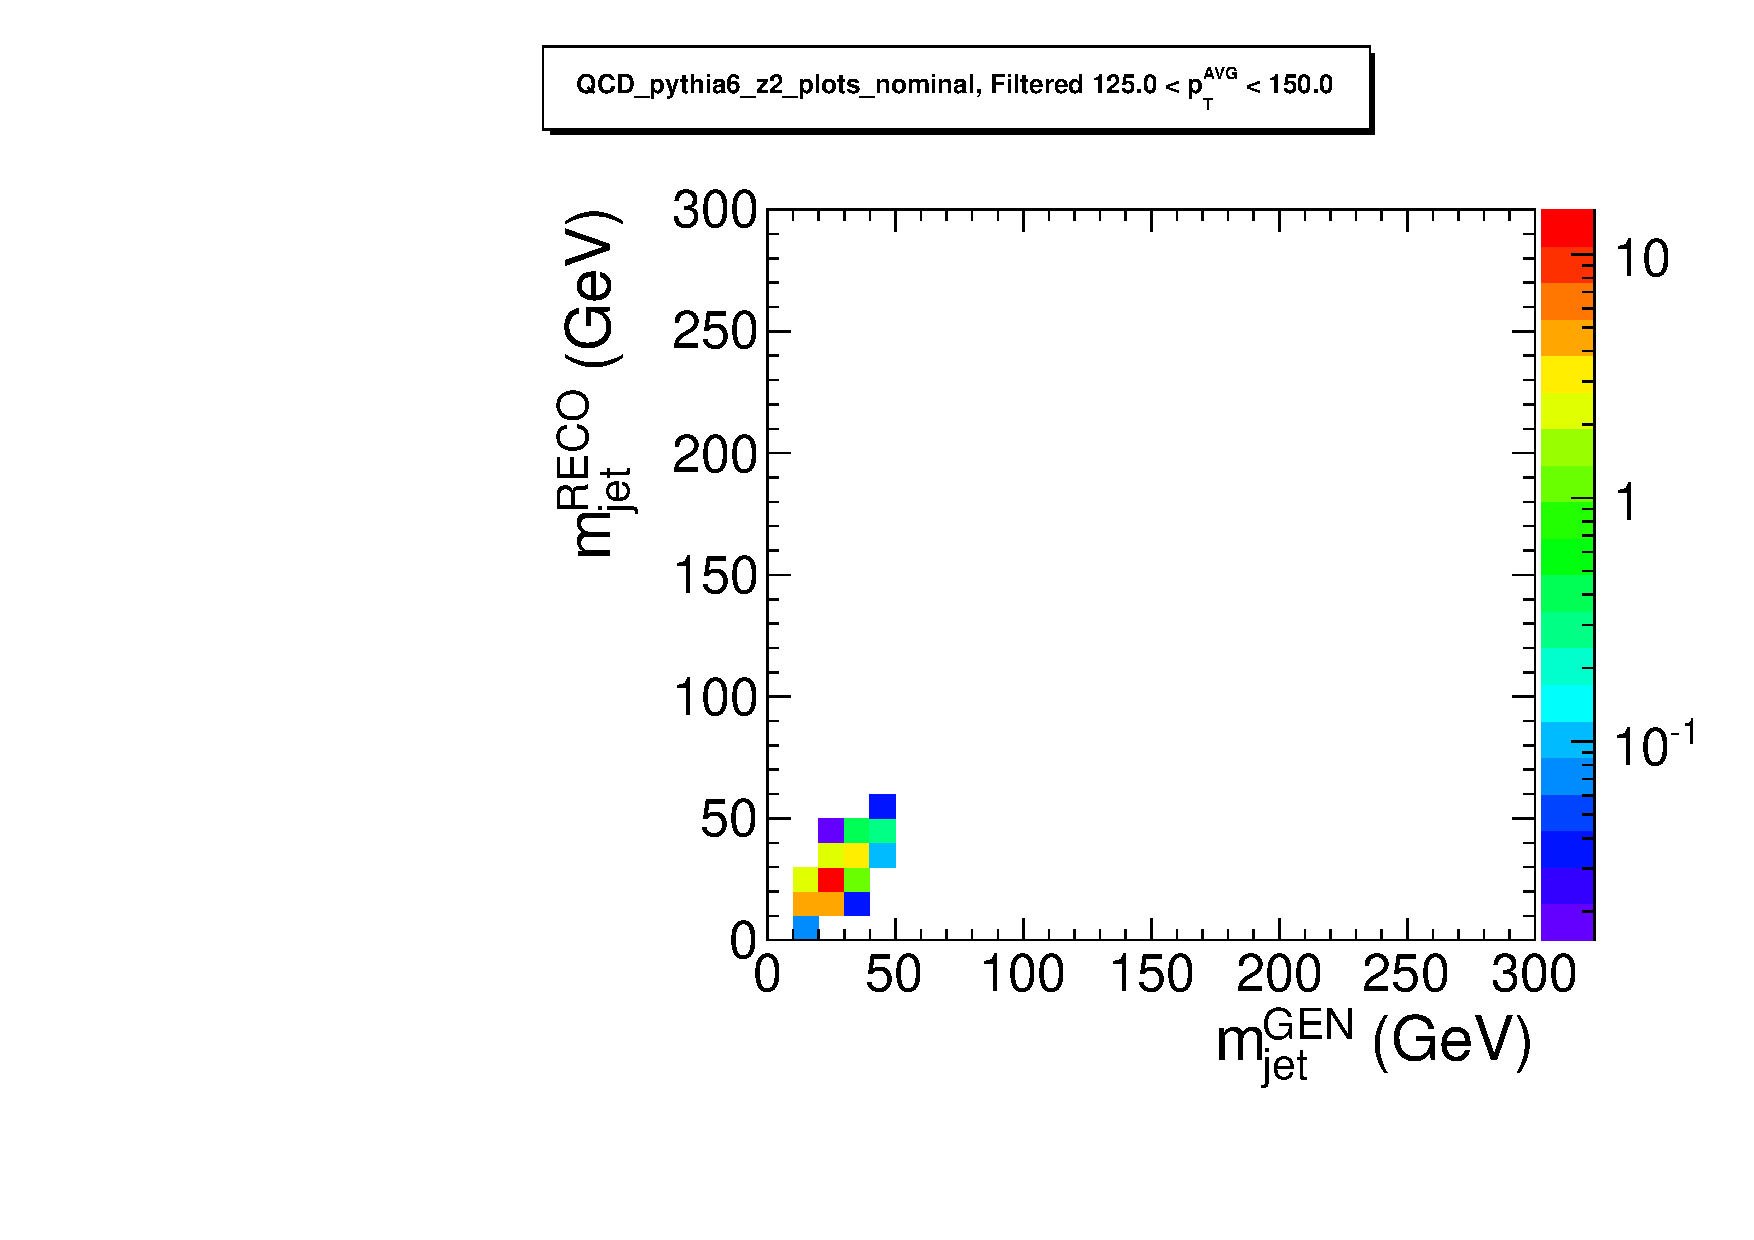
\includegraphics[width=0.3\textwidth]{figs/response_QCD_pythia6_z2_plots_nominal_Filtered_pt2}}
\subfigure{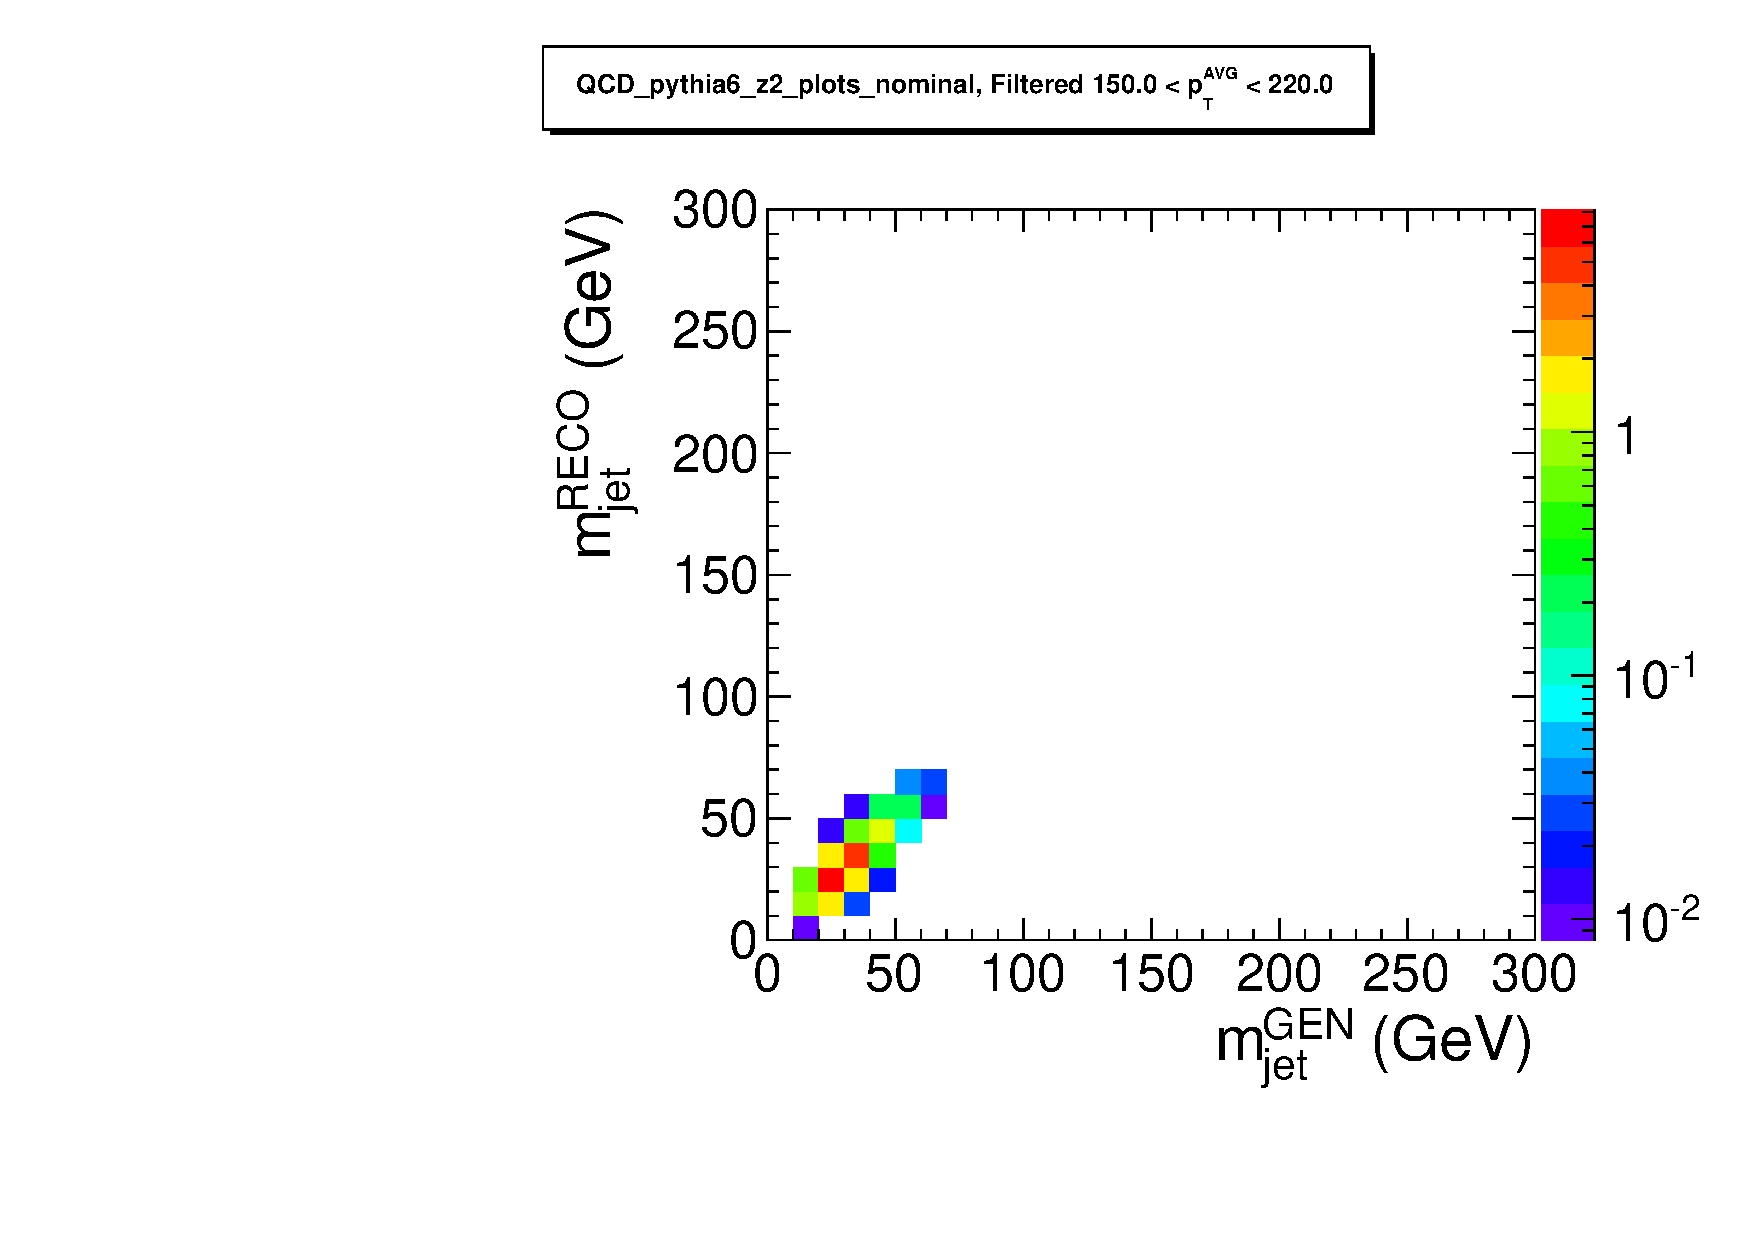
\includegraphics[width=0.3\textwidth]{figs/response_QCD_pythia6_z2_plots_nominal_Filtered_pt3}}\\
\subfigure{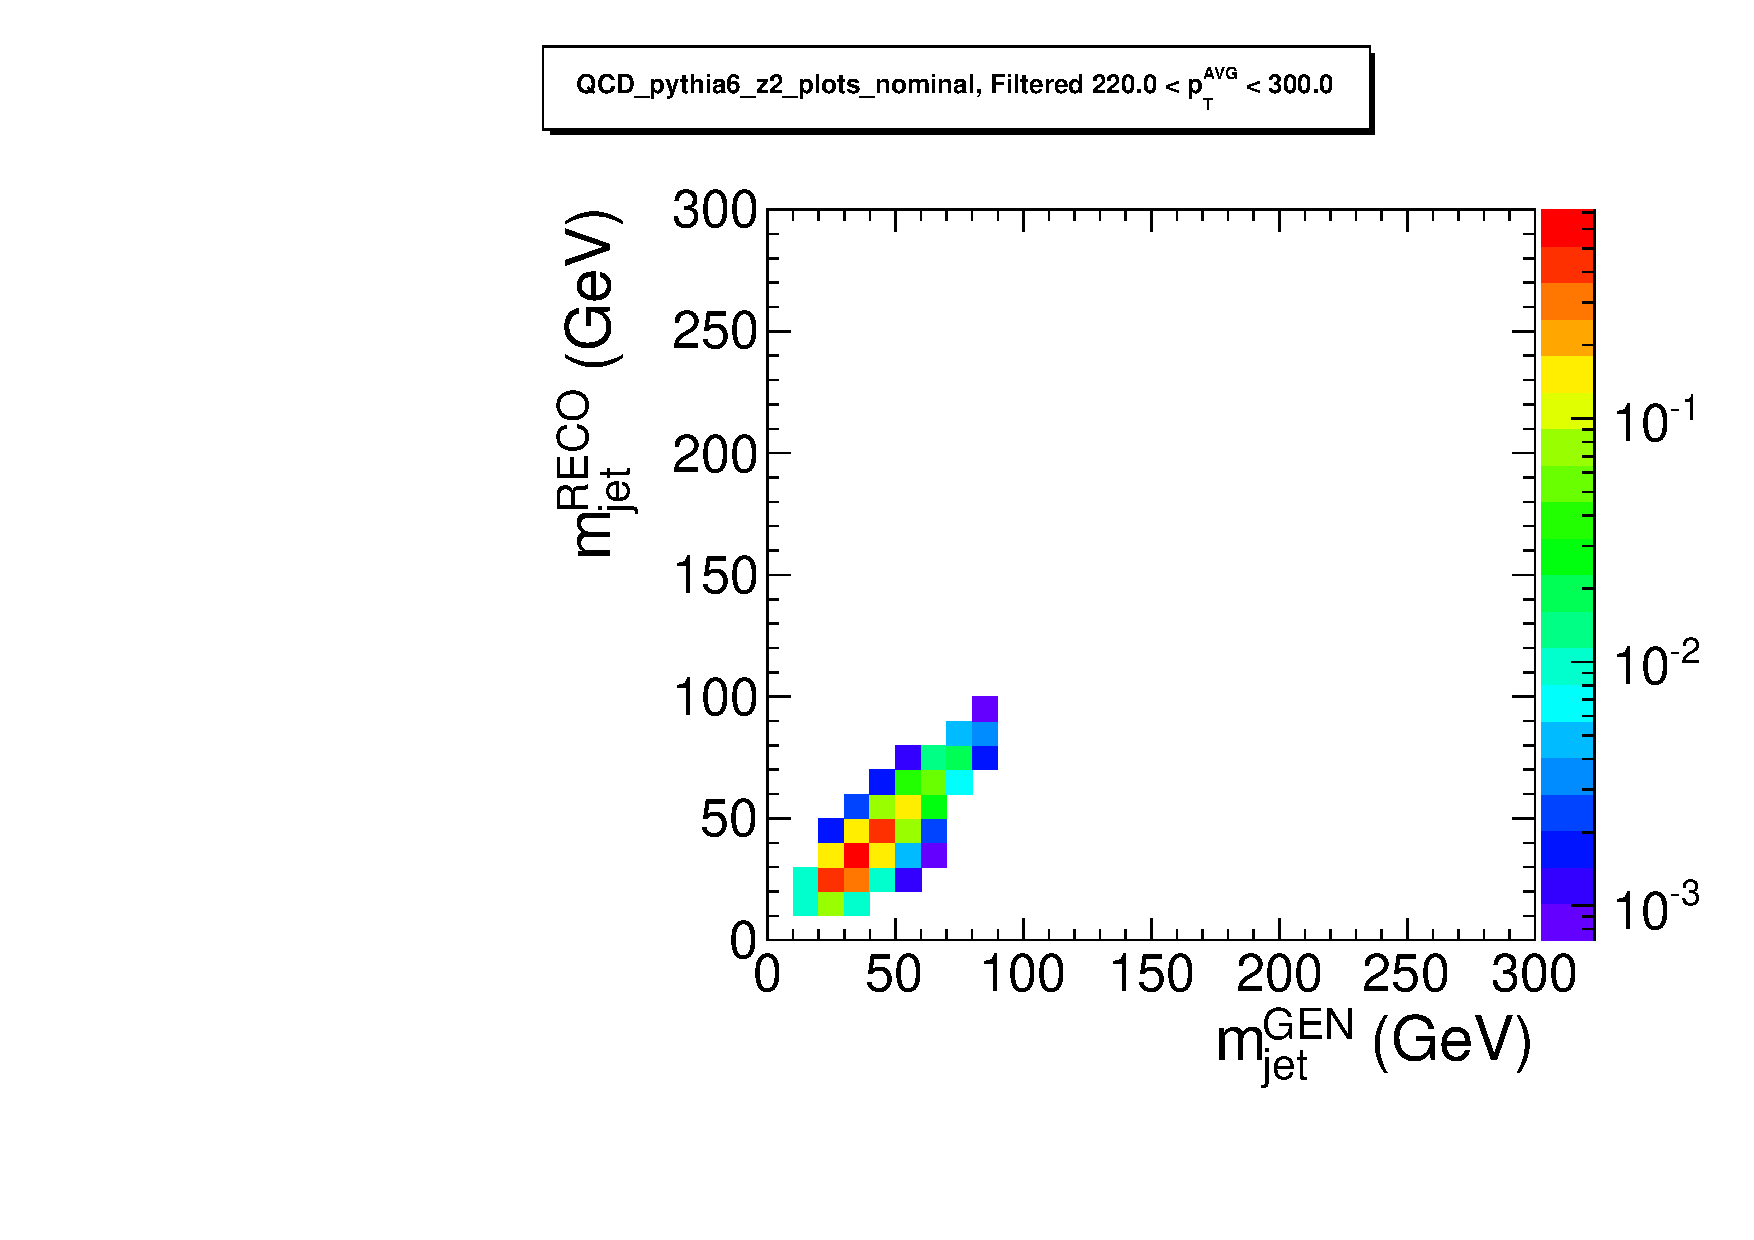
\includegraphics[width=0.3\textwidth]{figs/response_QCD_pythia6_z2_plots_nominal_Filtered_pt4}}
\subfigure{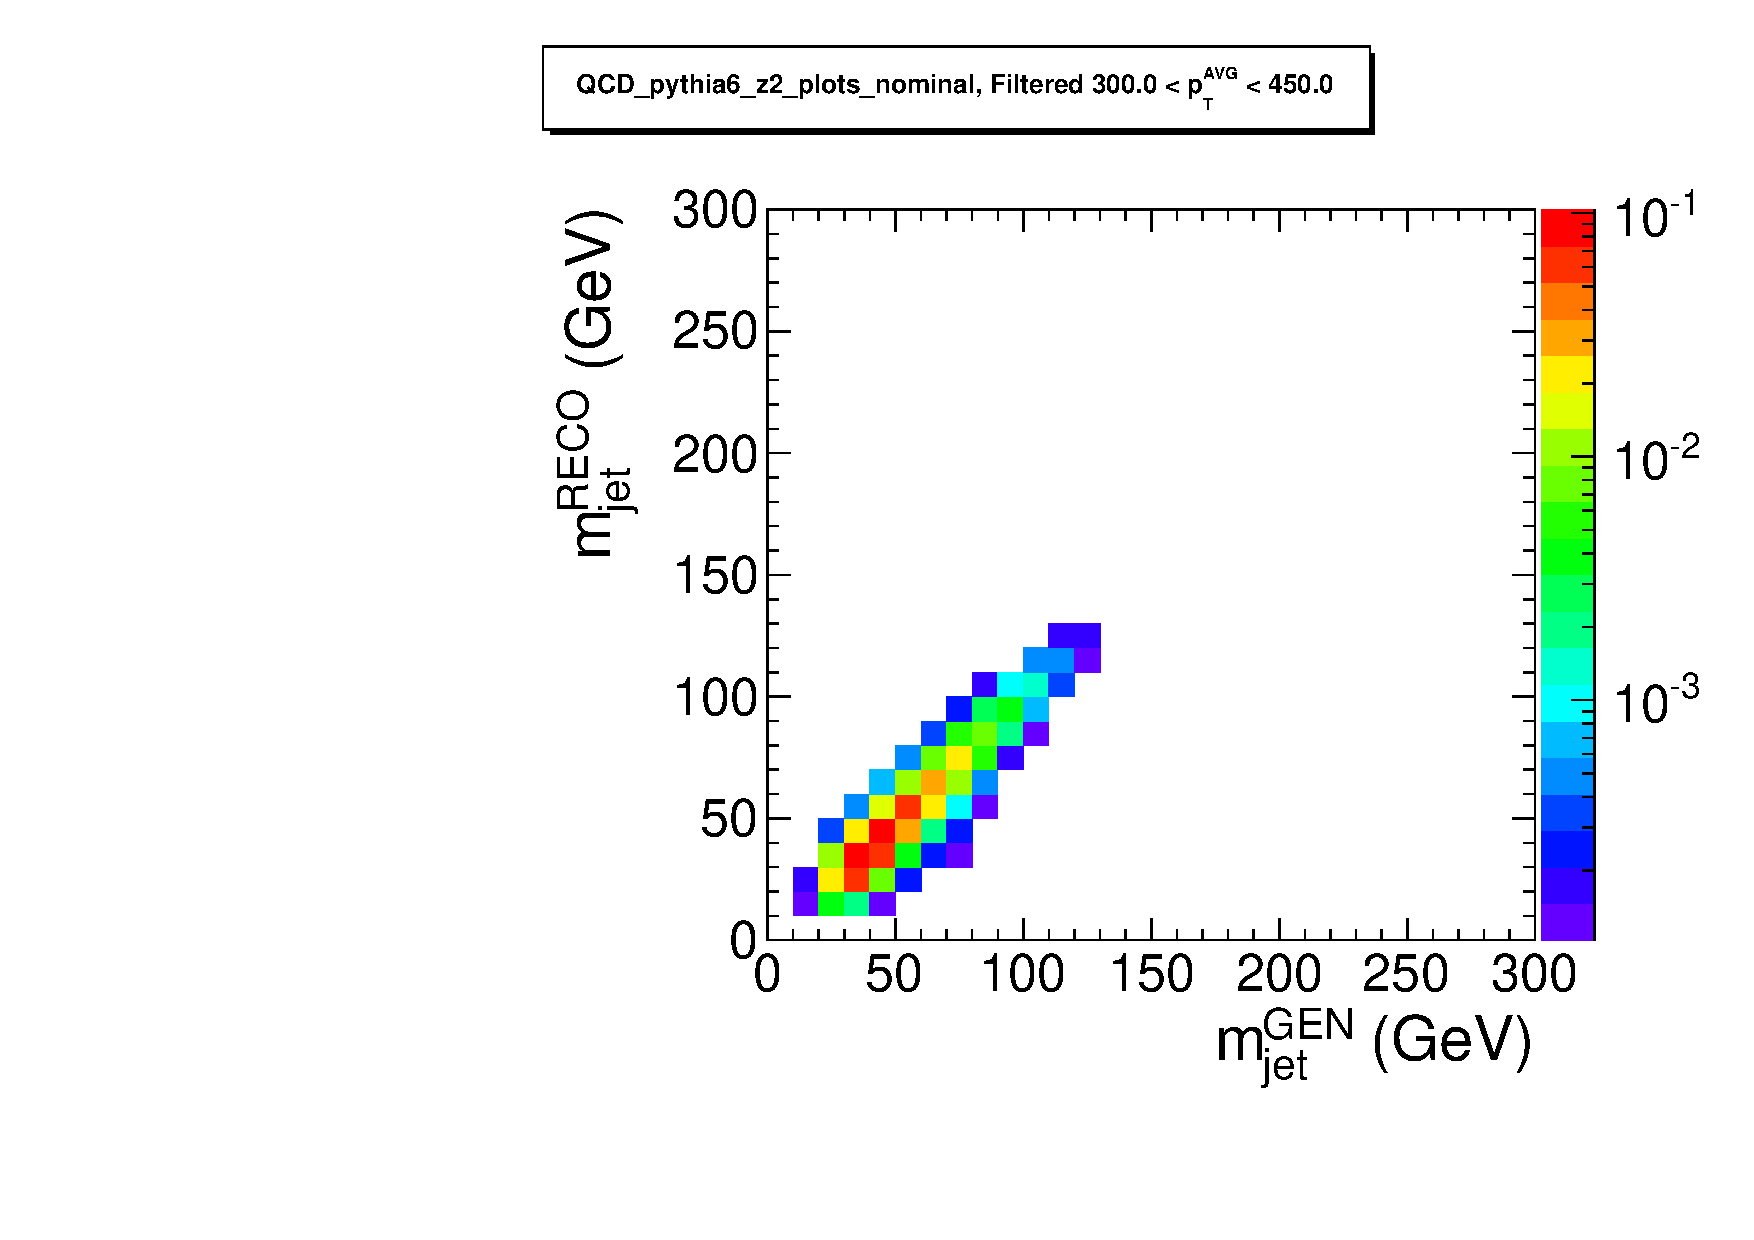
\includegraphics[width=0.3\textwidth]{figs/response_QCD_pythia6_z2_plots_nominal_Filtered_pt5}}
\subfigure{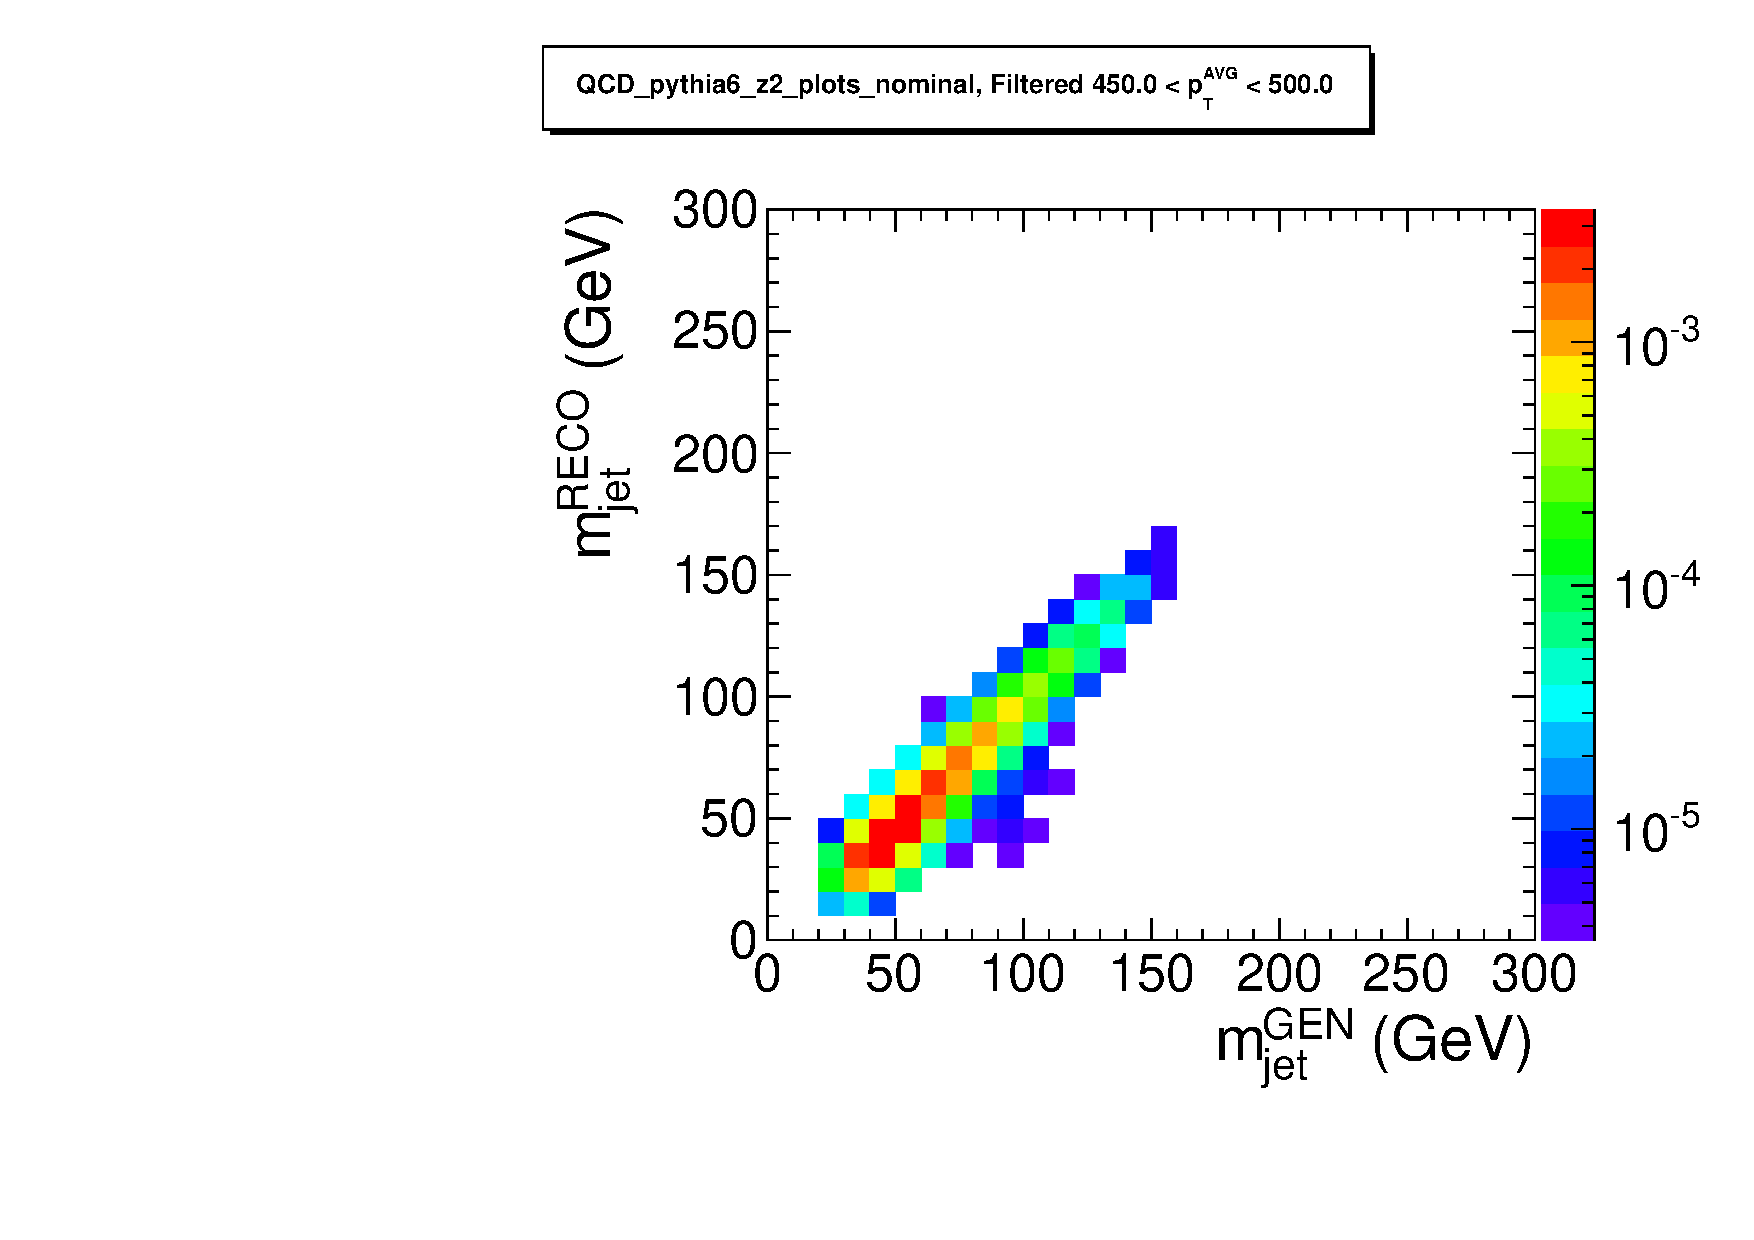
\includegraphics[width=0.3\textwidth]{figs/response_QCD_pythia6_z2_plots_nominal_Filtered_pt6}}\\
\subfigure{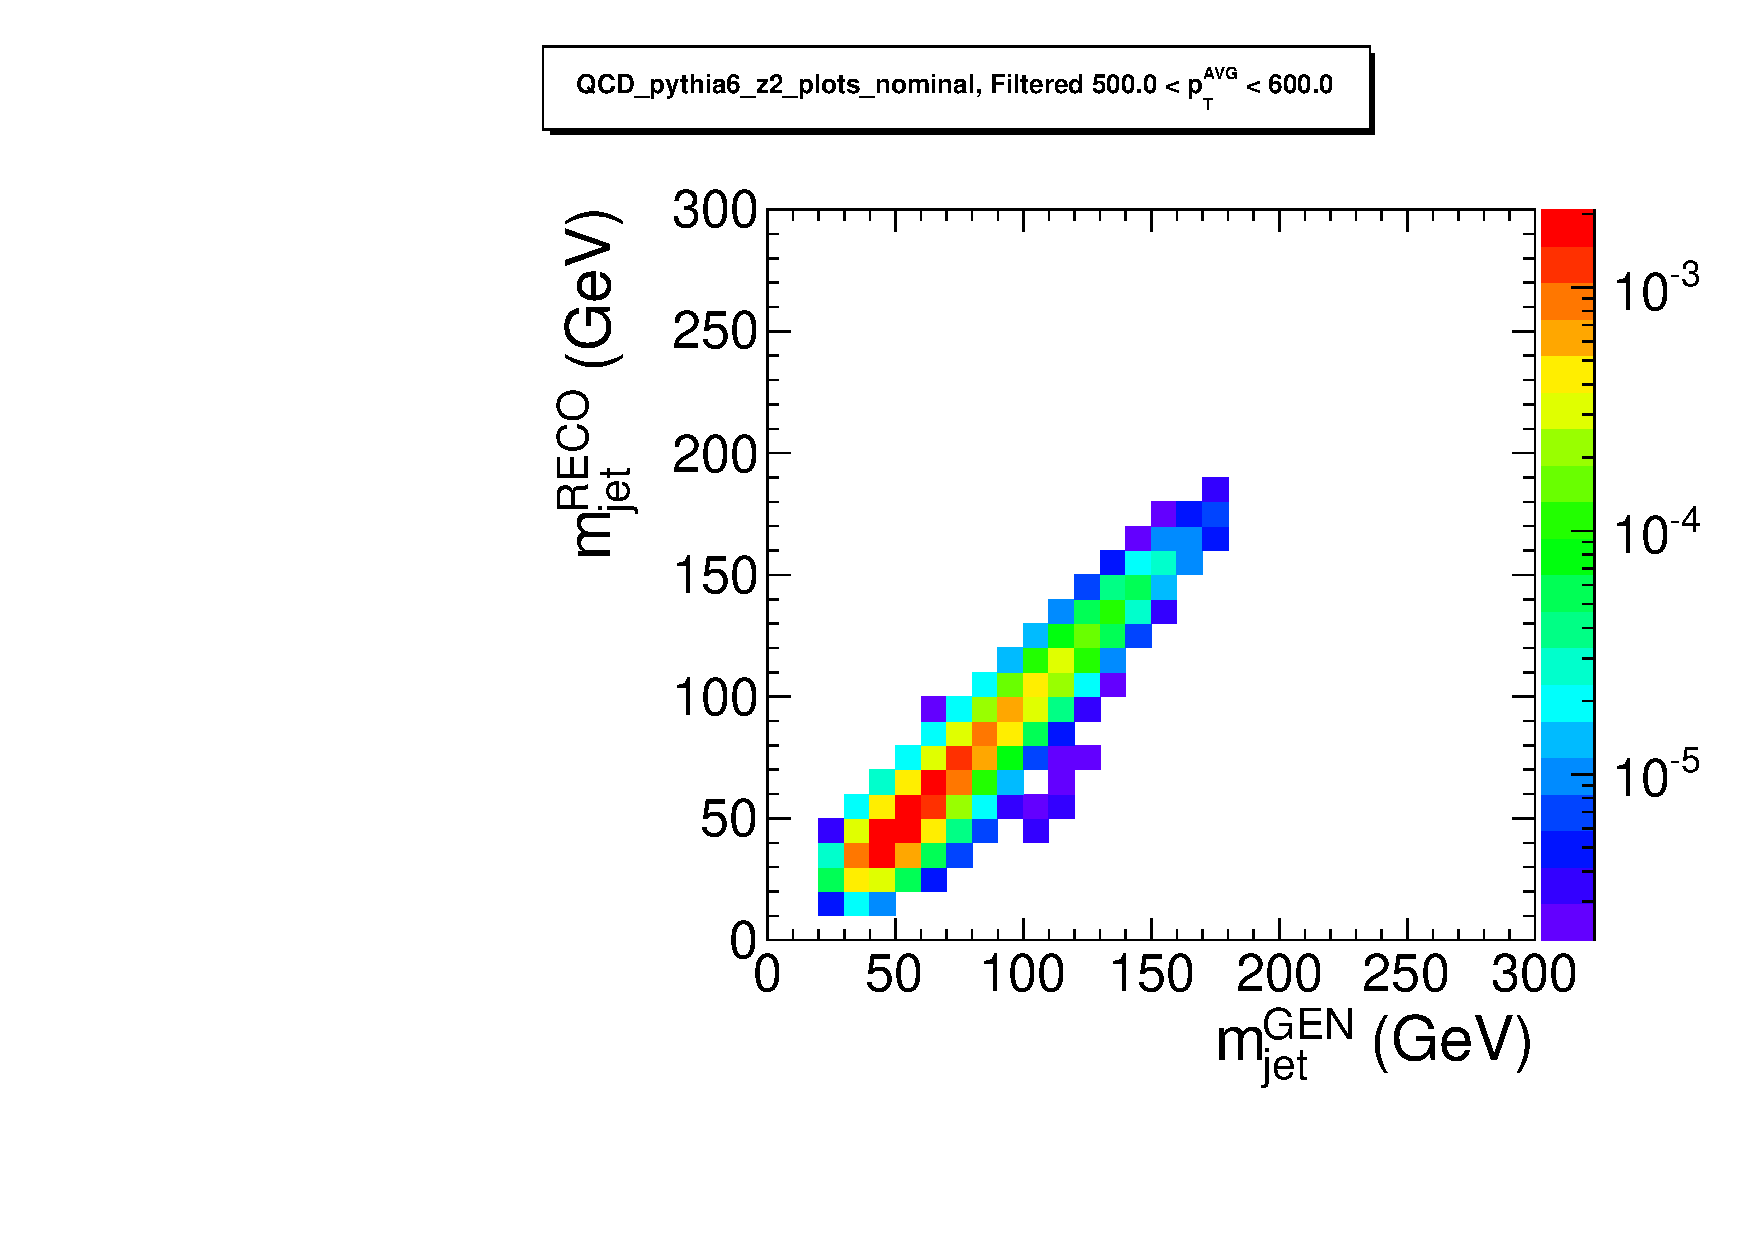
\includegraphics[width=0.3\textwidth]{figs/response_QCD_pythia6_z2_plots_nominal_Filtered_pt7}}
\subfigure{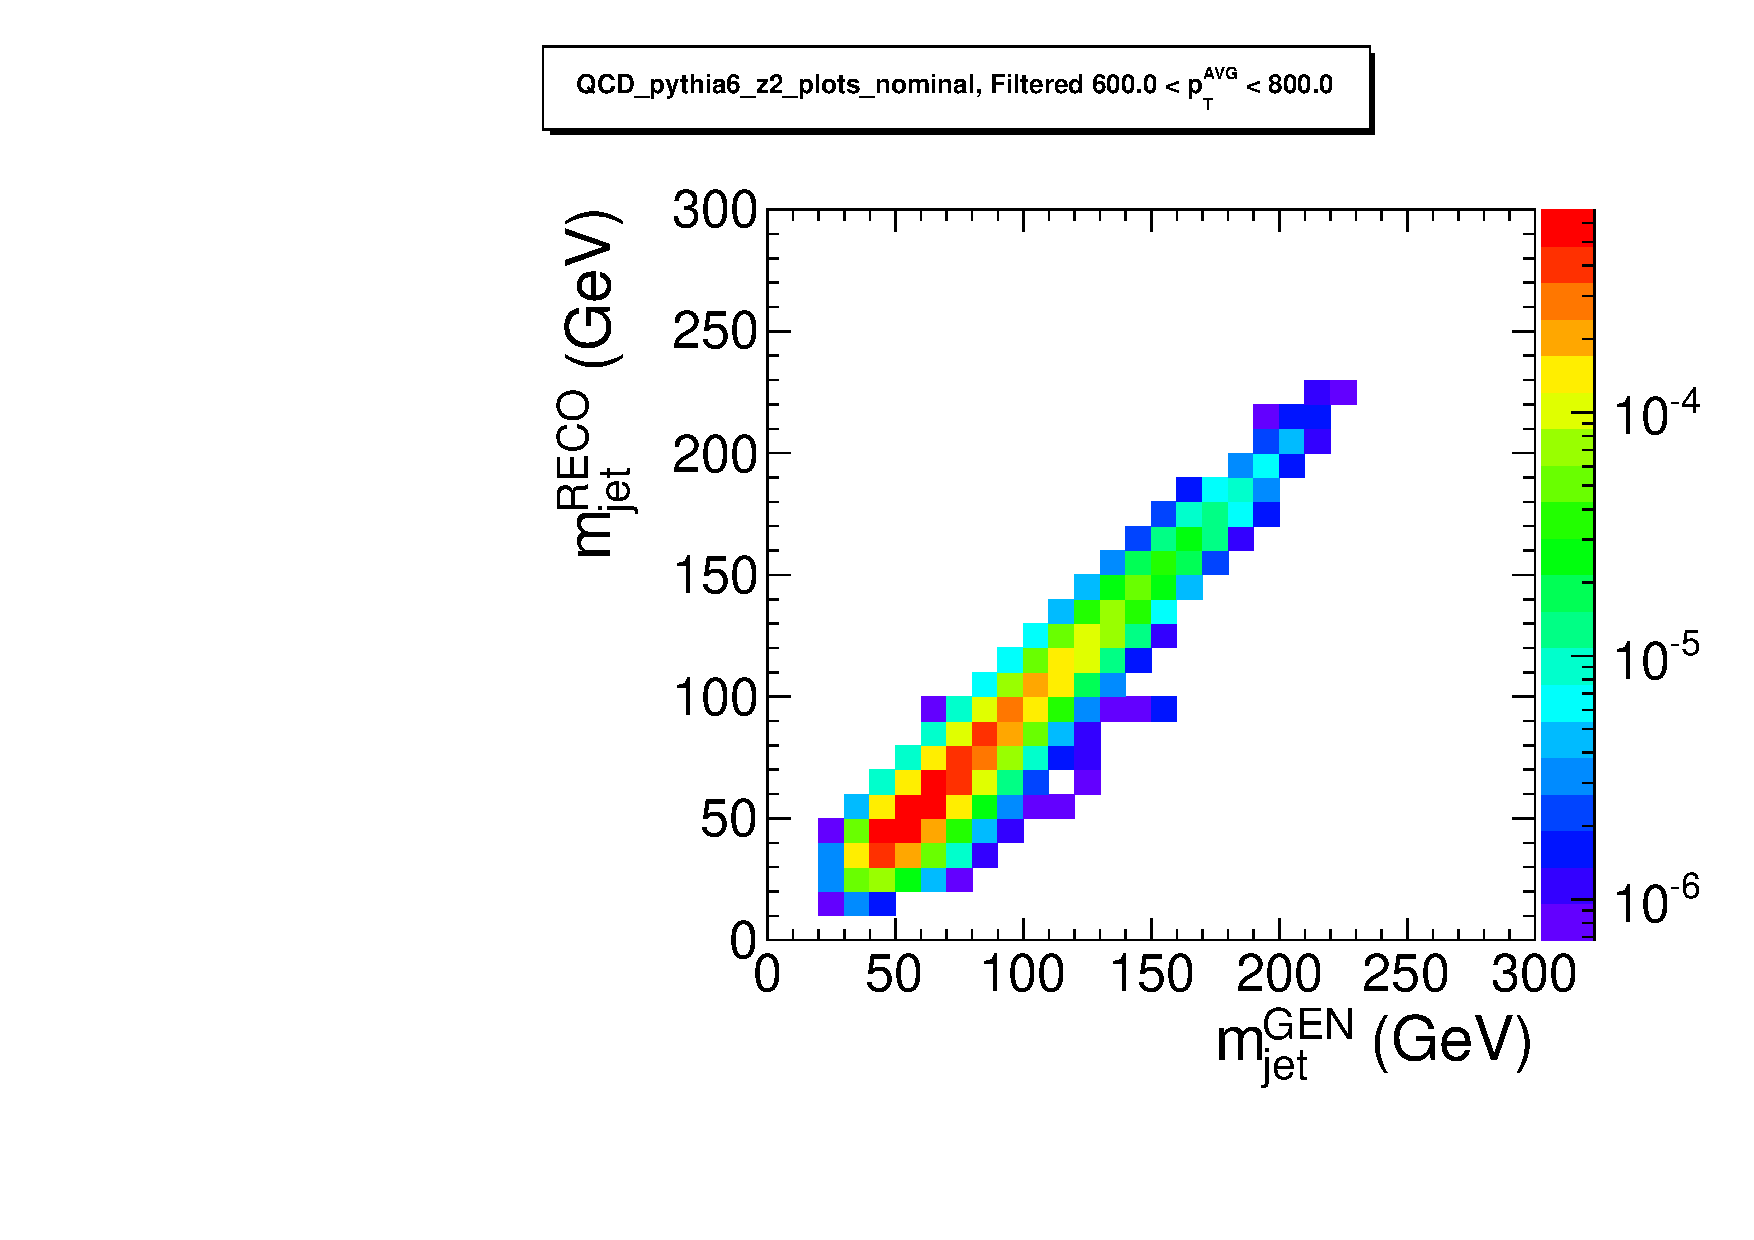
\includegraphics[width=0.3\textwidth]{figs/response_QCD_pythia6_z2_plots_nominal_Filtered_pt8}}
\subfigure{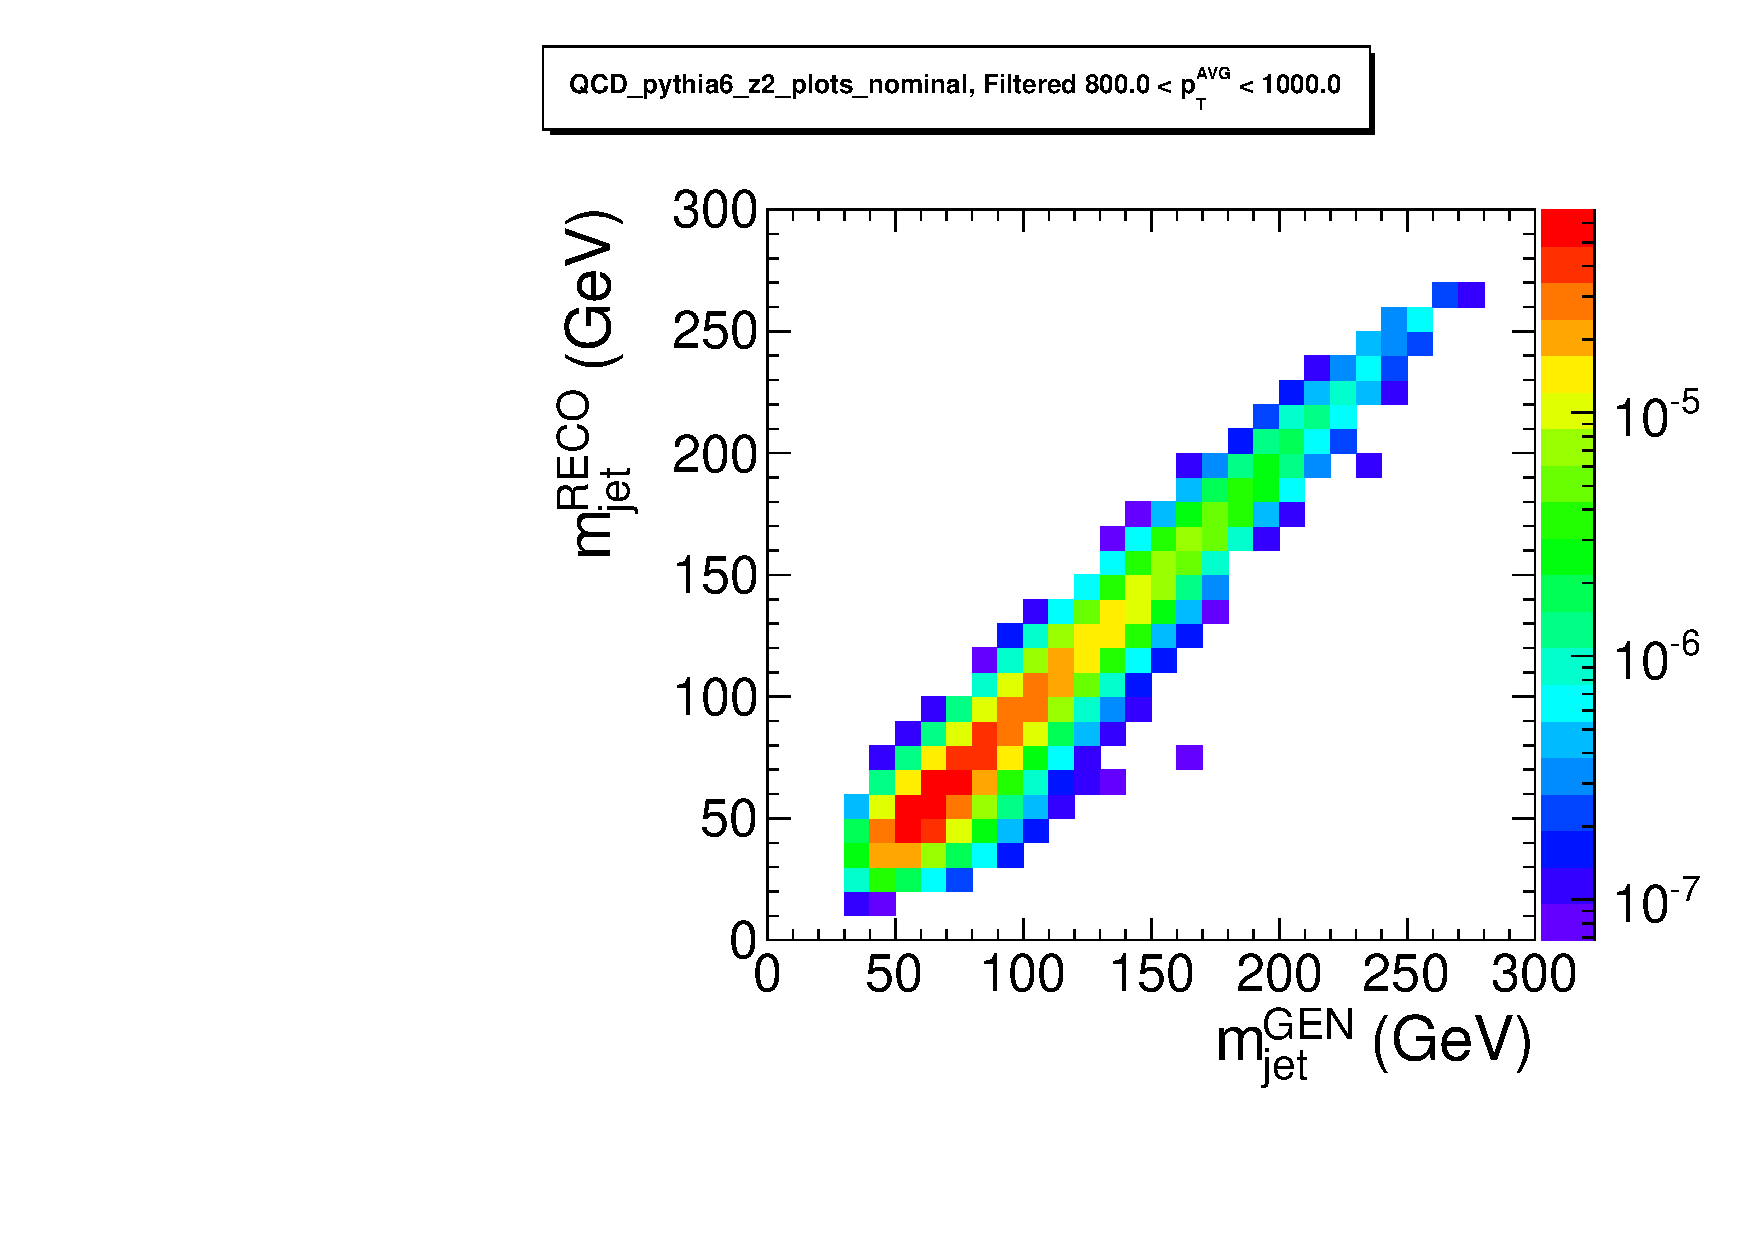
\includegraphics[width=0.3\textwidth]{figs/response_QCD_pythia6_z2_plots_nominal_Filtered_pt9}}\\
\caption{Response of the jet mass for AK7 Filteredjets,
for various $\pt^{AVG}$ bins. The true jet mass is shown
on the $x-$axis, and the reconstructed jet mass is shown on the
$y-$axis, using the \PYTHIA generator. 
\label{figs:response_QCD_pythia6_z2_plots_nominal_Filtered_ptall}}
\end{figure}


\clearpage

\begin{figure}[htbp]
\centering
\subfigure{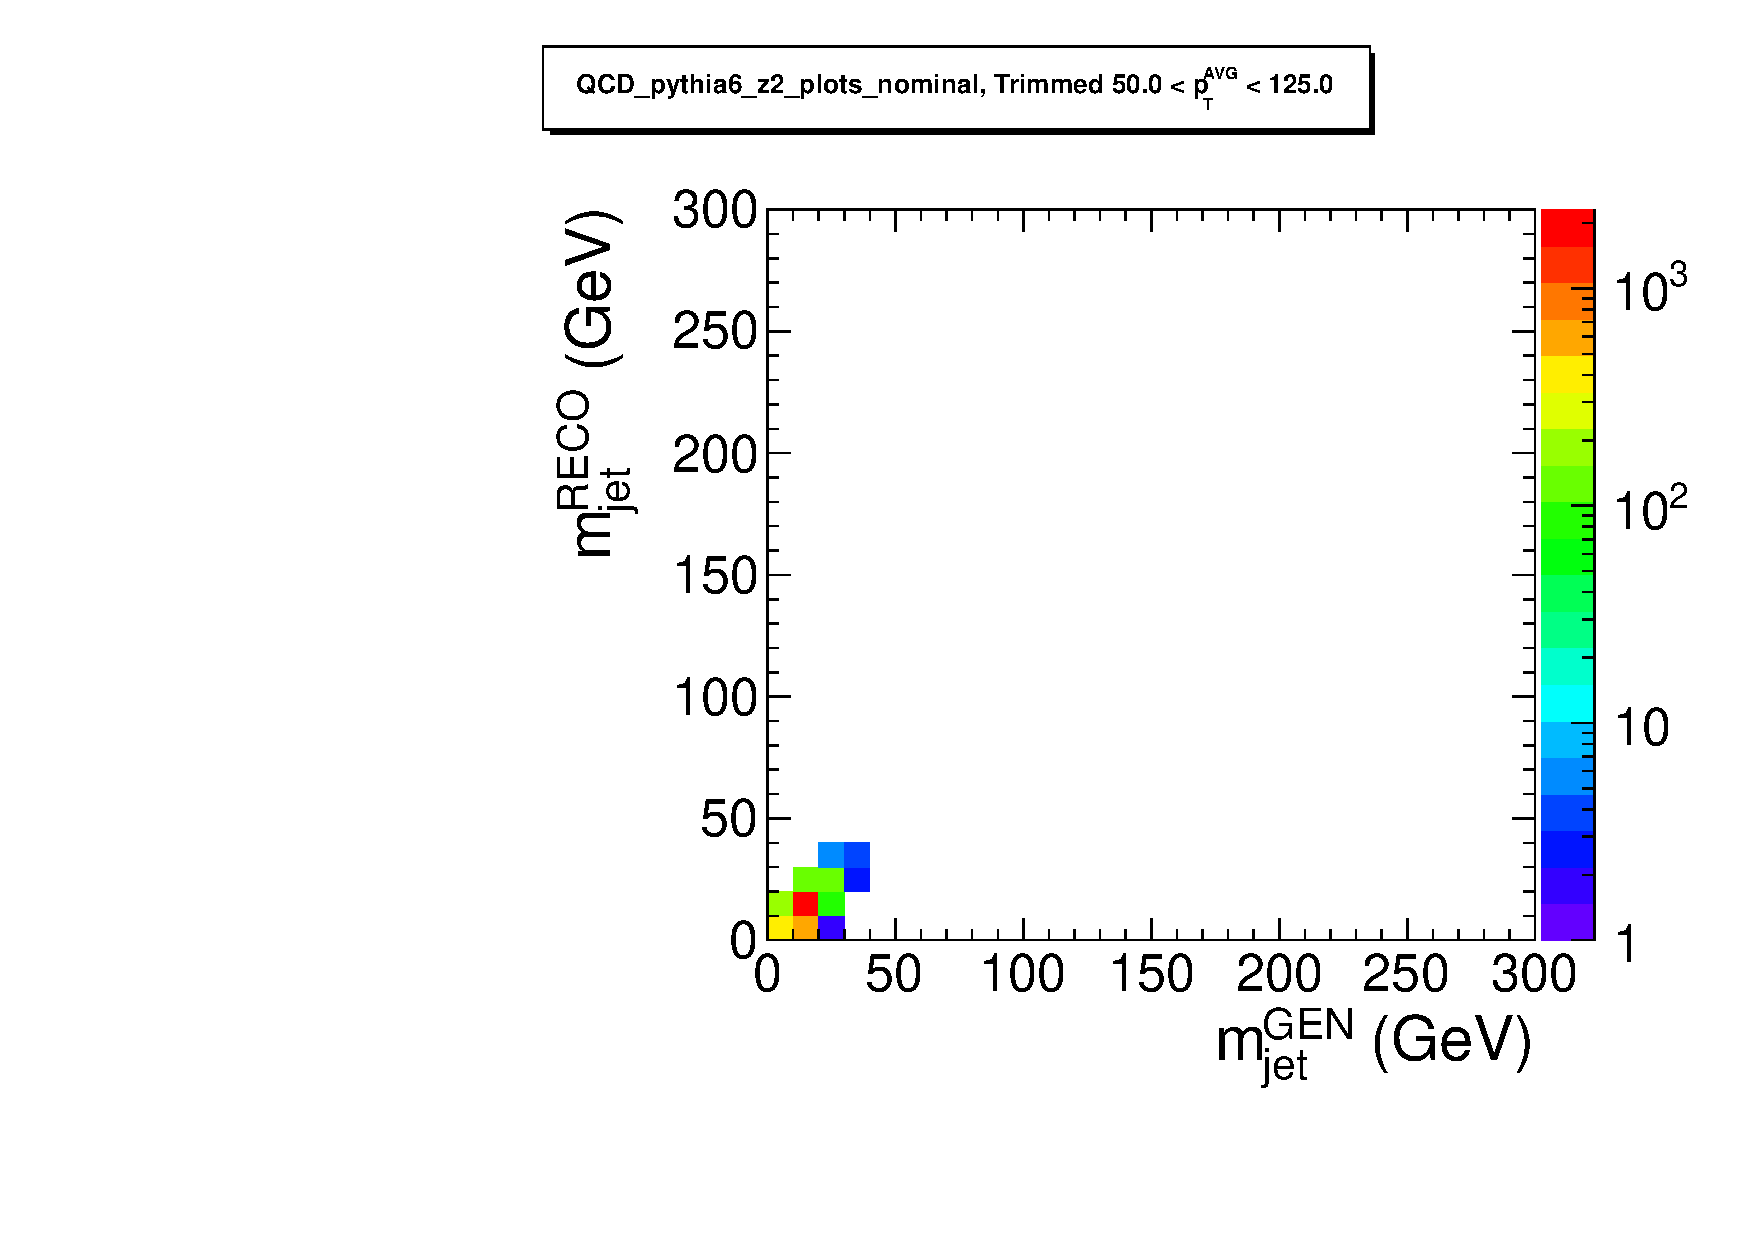
\includegraphics[width=0.3\textwidth]{figs/response_QCD_pythia6_z2_plots_nominal_Trimmed_pt1}}
\subfigure{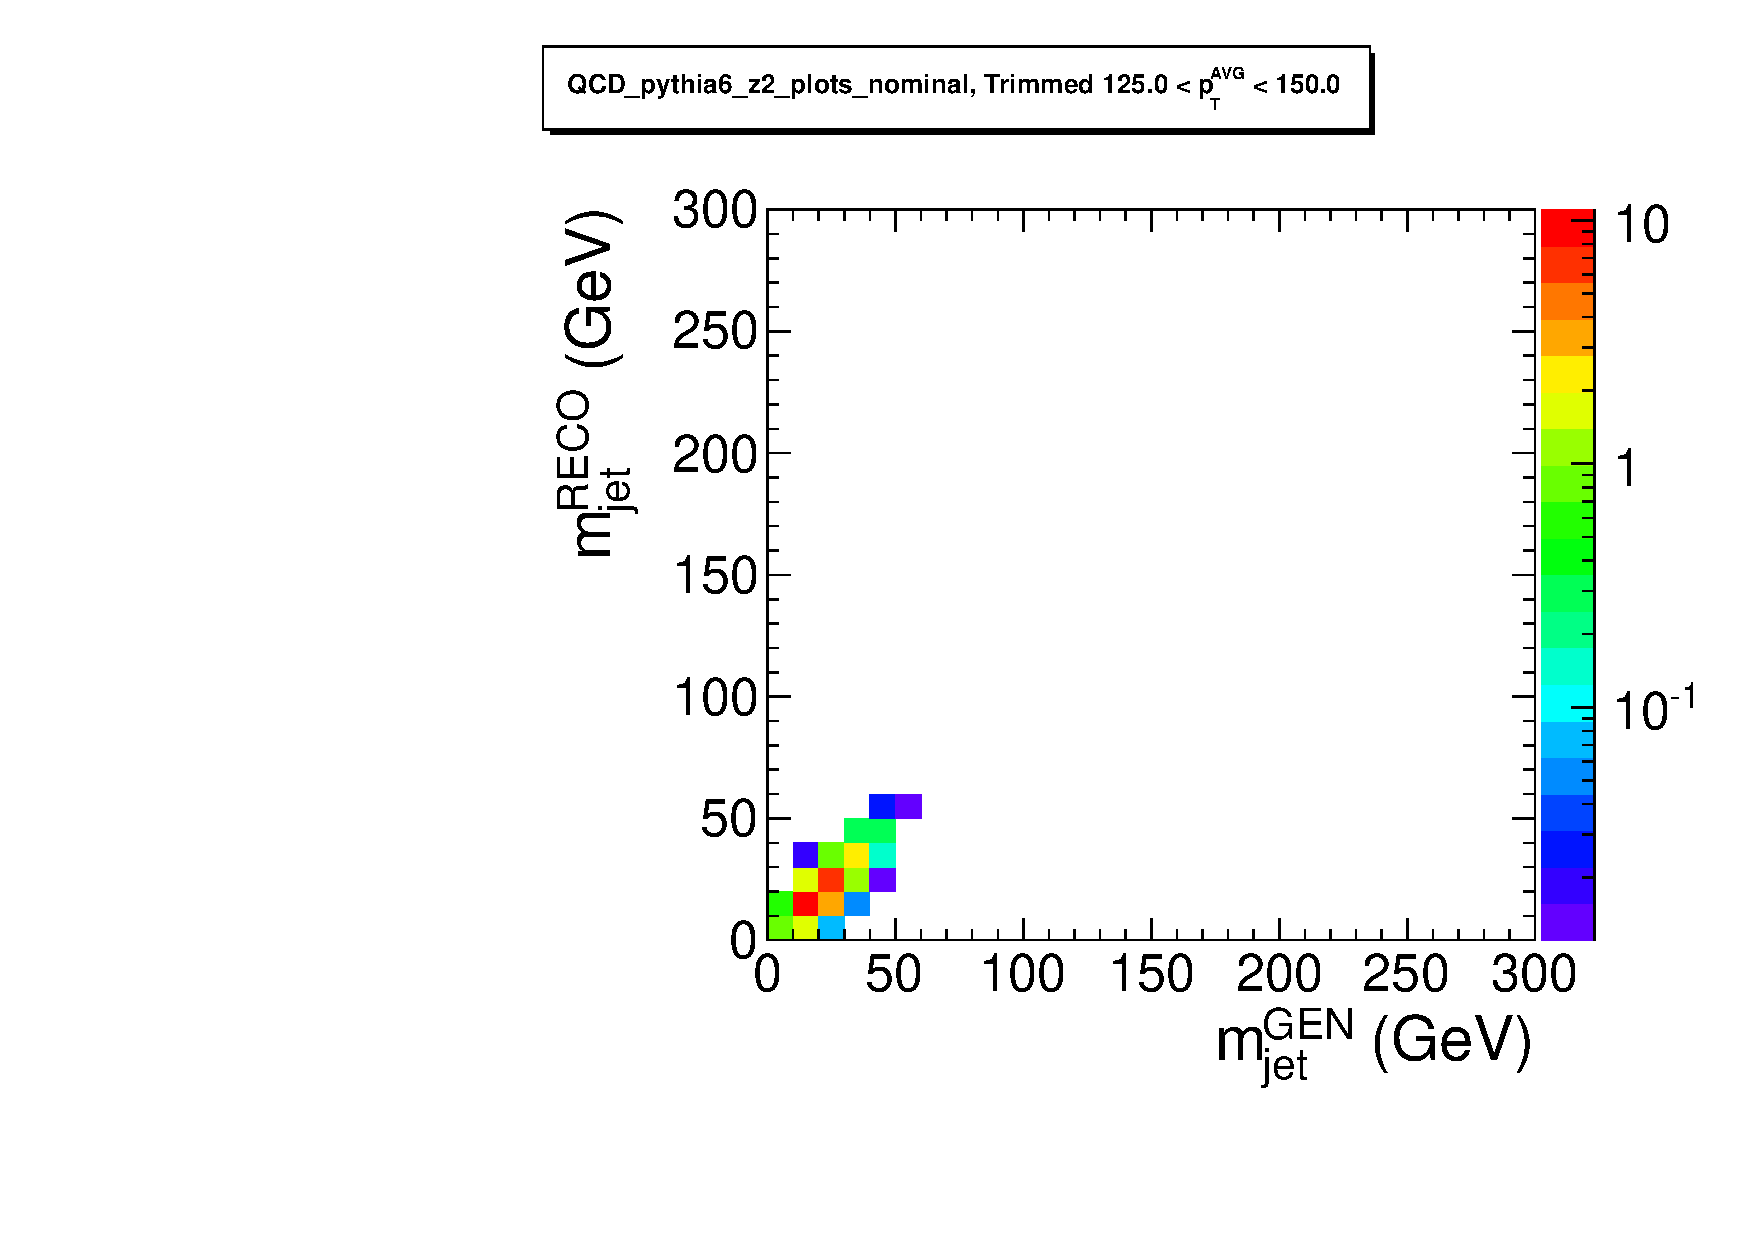
\includegraphics[width=0.3\textwidth]{figs/response_QCD_pythia6_z2_plots_nominal_Trimmed_pt2}}
\subfigure{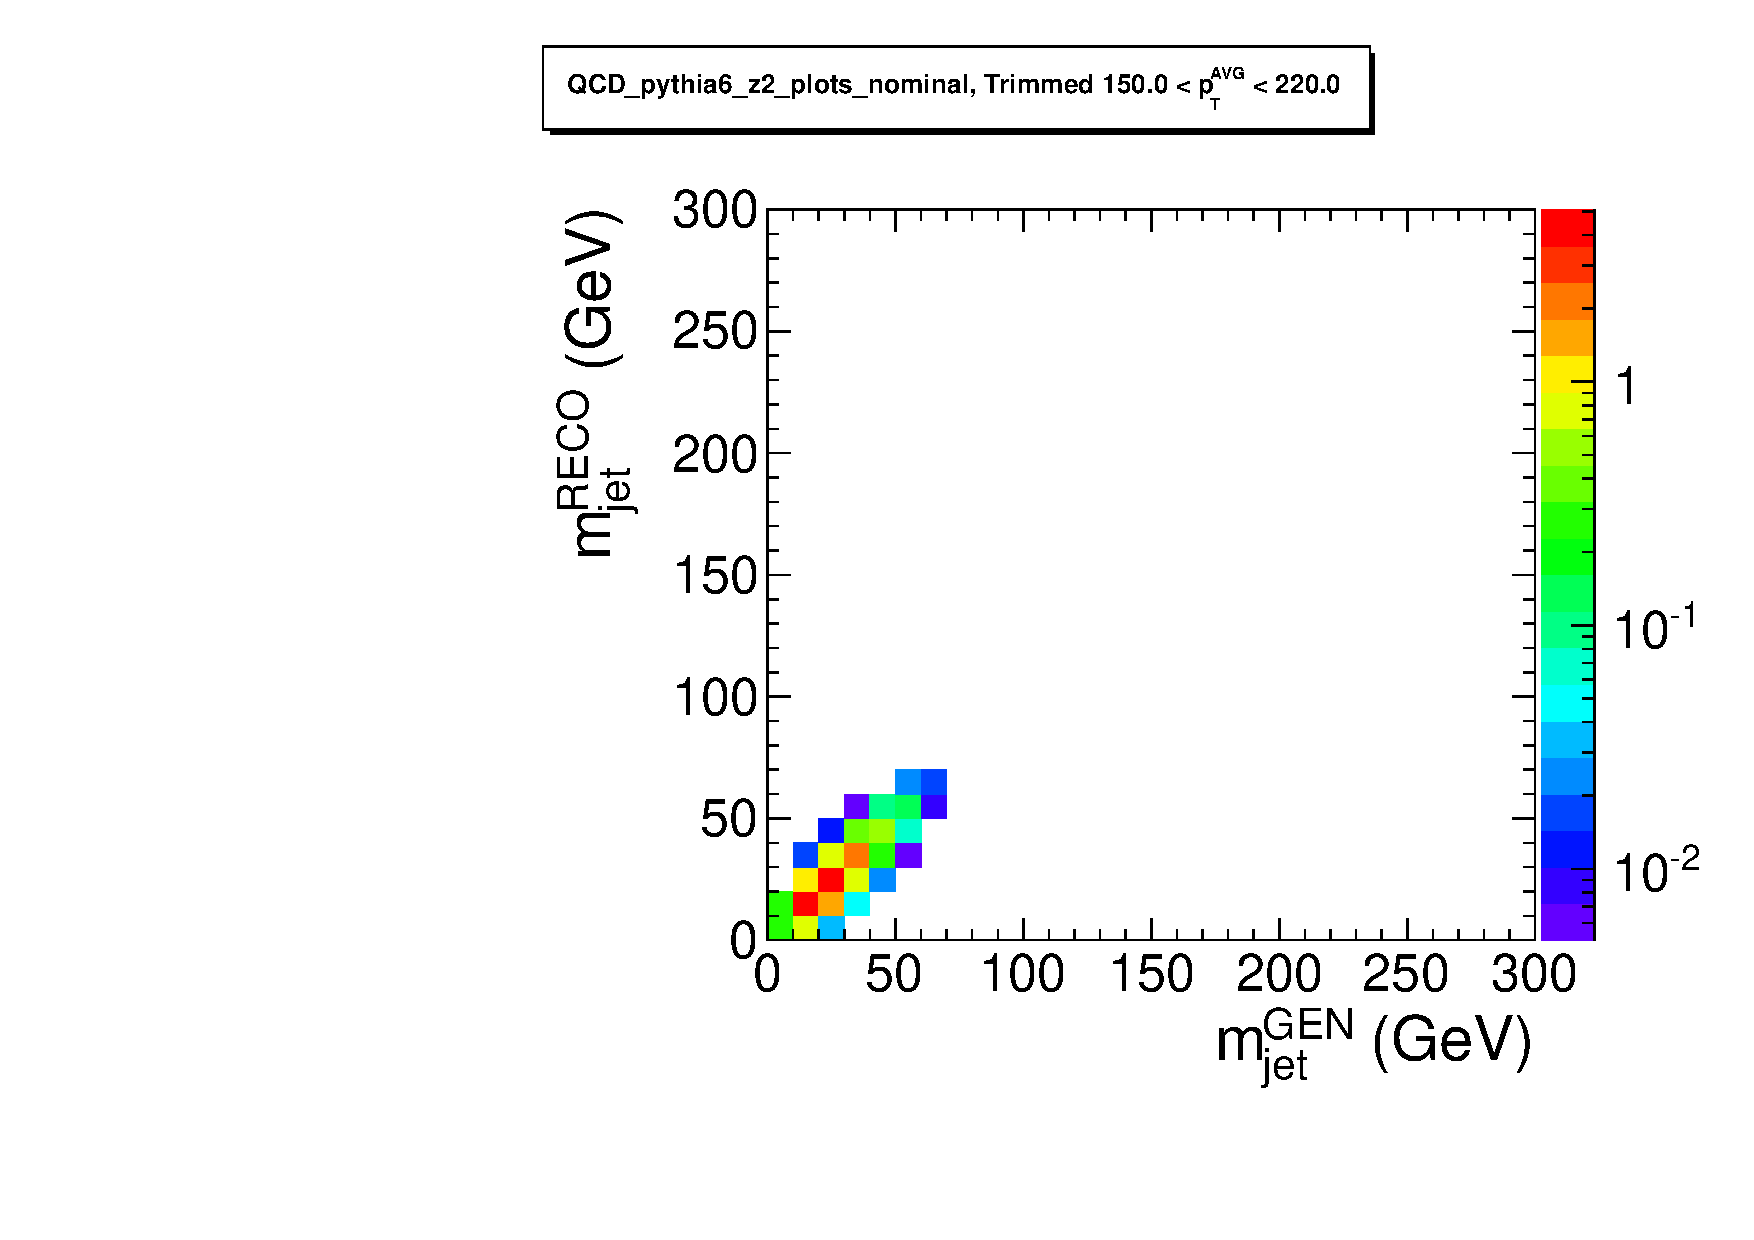
\includegraphics[width=0.3\textwidth]{figs/response_QCD_pythia6_z2_plots_nominal_Trimmed_pt3}}\\
\subfigure{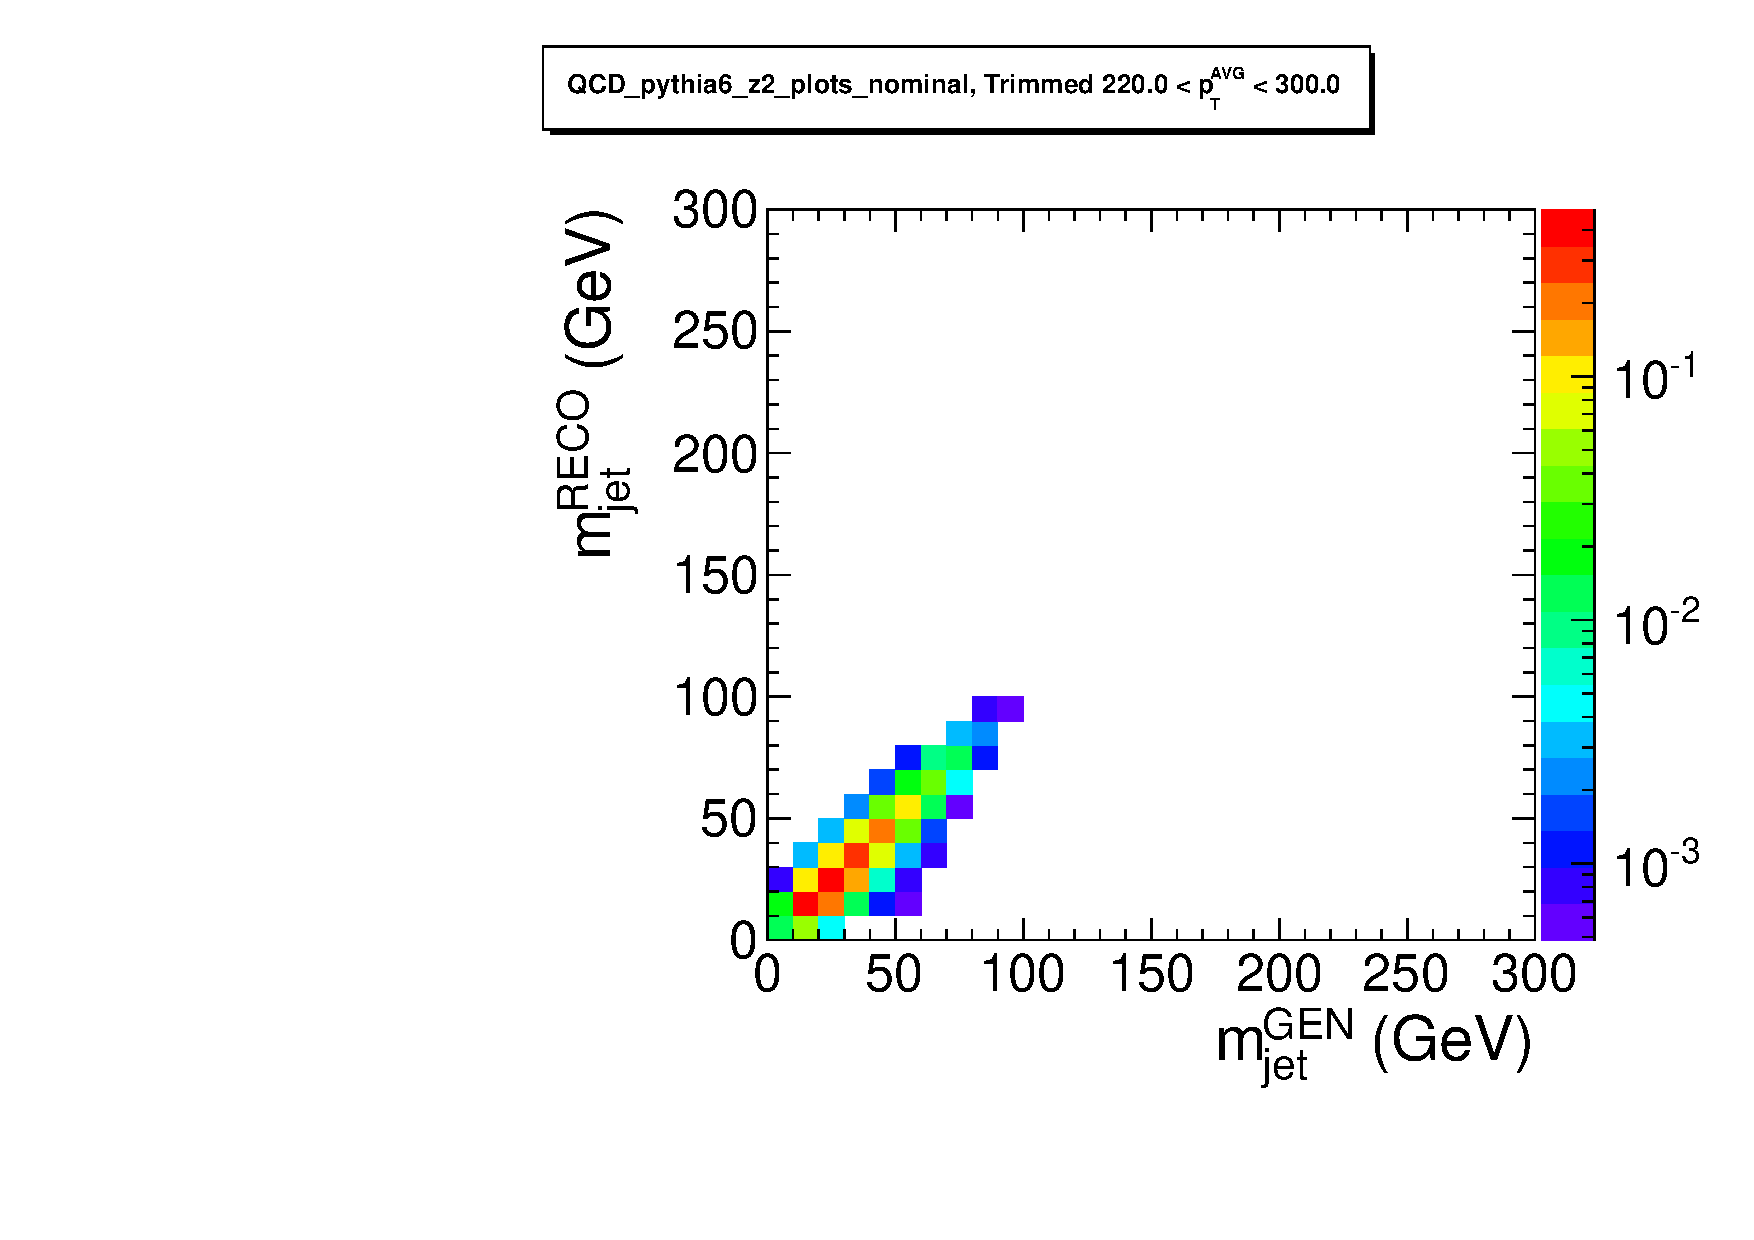
\includegraphics[width=0.3\textwidth]{figs/response_QCD_pythia6_z2_plots_nominal_Trimmed_pt4}}
\subfigure{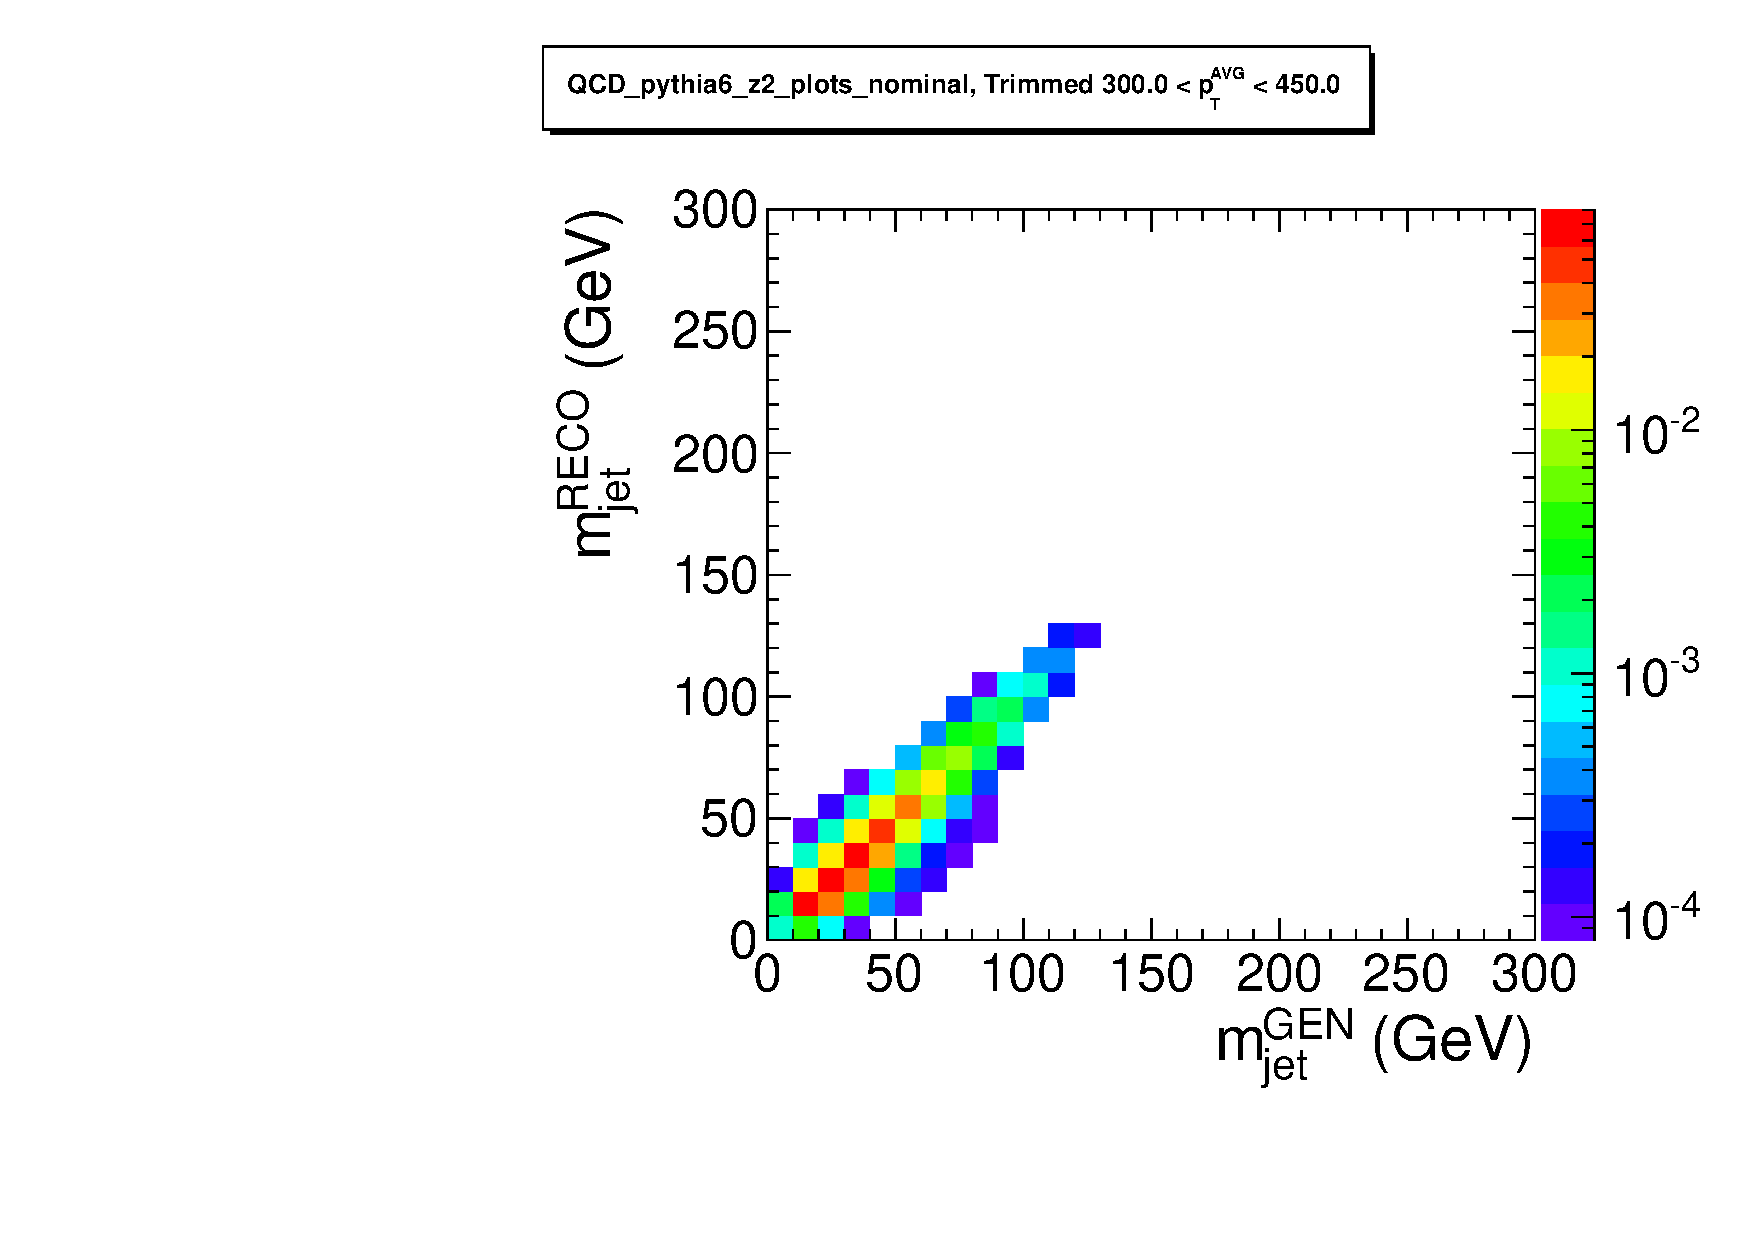
\includegraphics[width=0.3\textwidth]{figs/response_QCD_pythia6_z2_plots_nominal_Trimmed_pt5}}
\subfigure{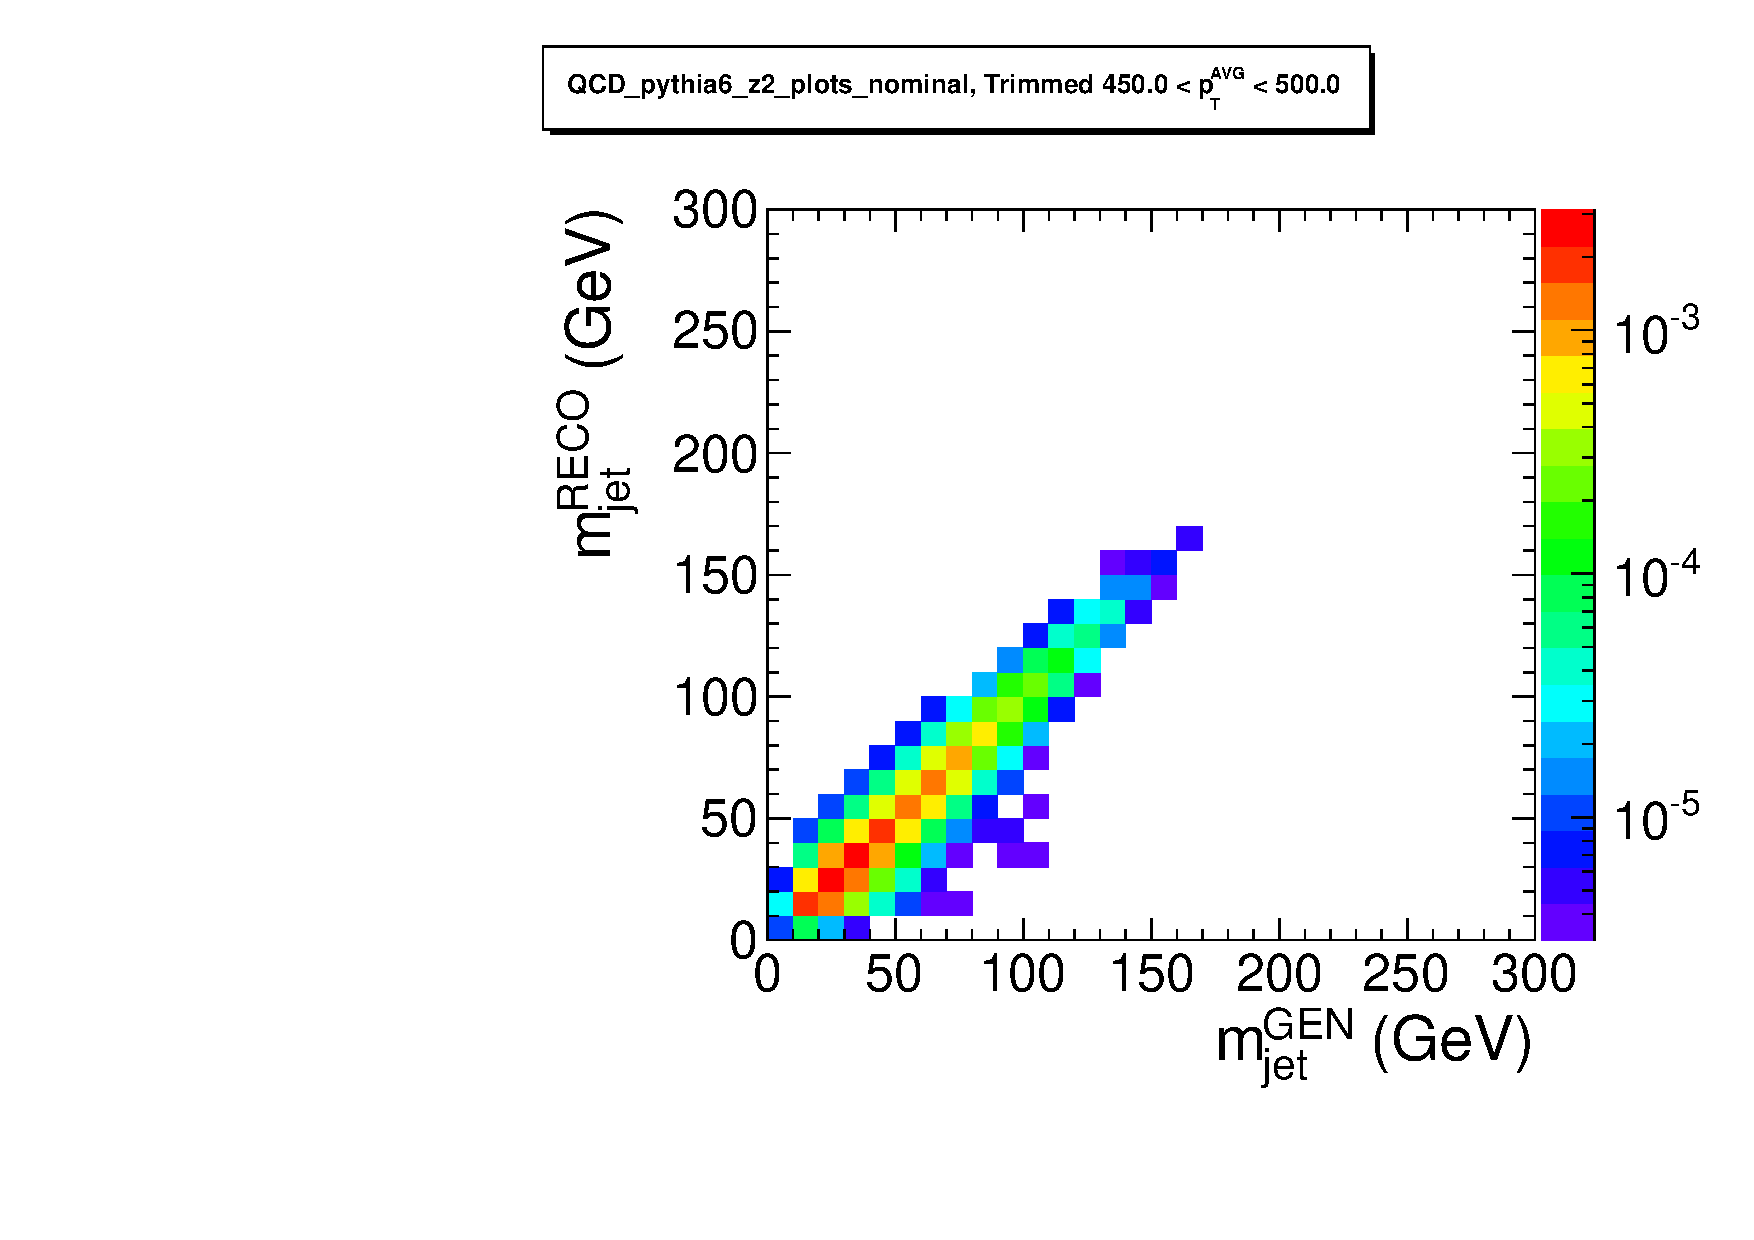
\includegraphics[width=0.3\textwidth]{figs/response_QCD_pythia6_z2_plots_nominal_Trimmed_pt6}}\\
\subfigure{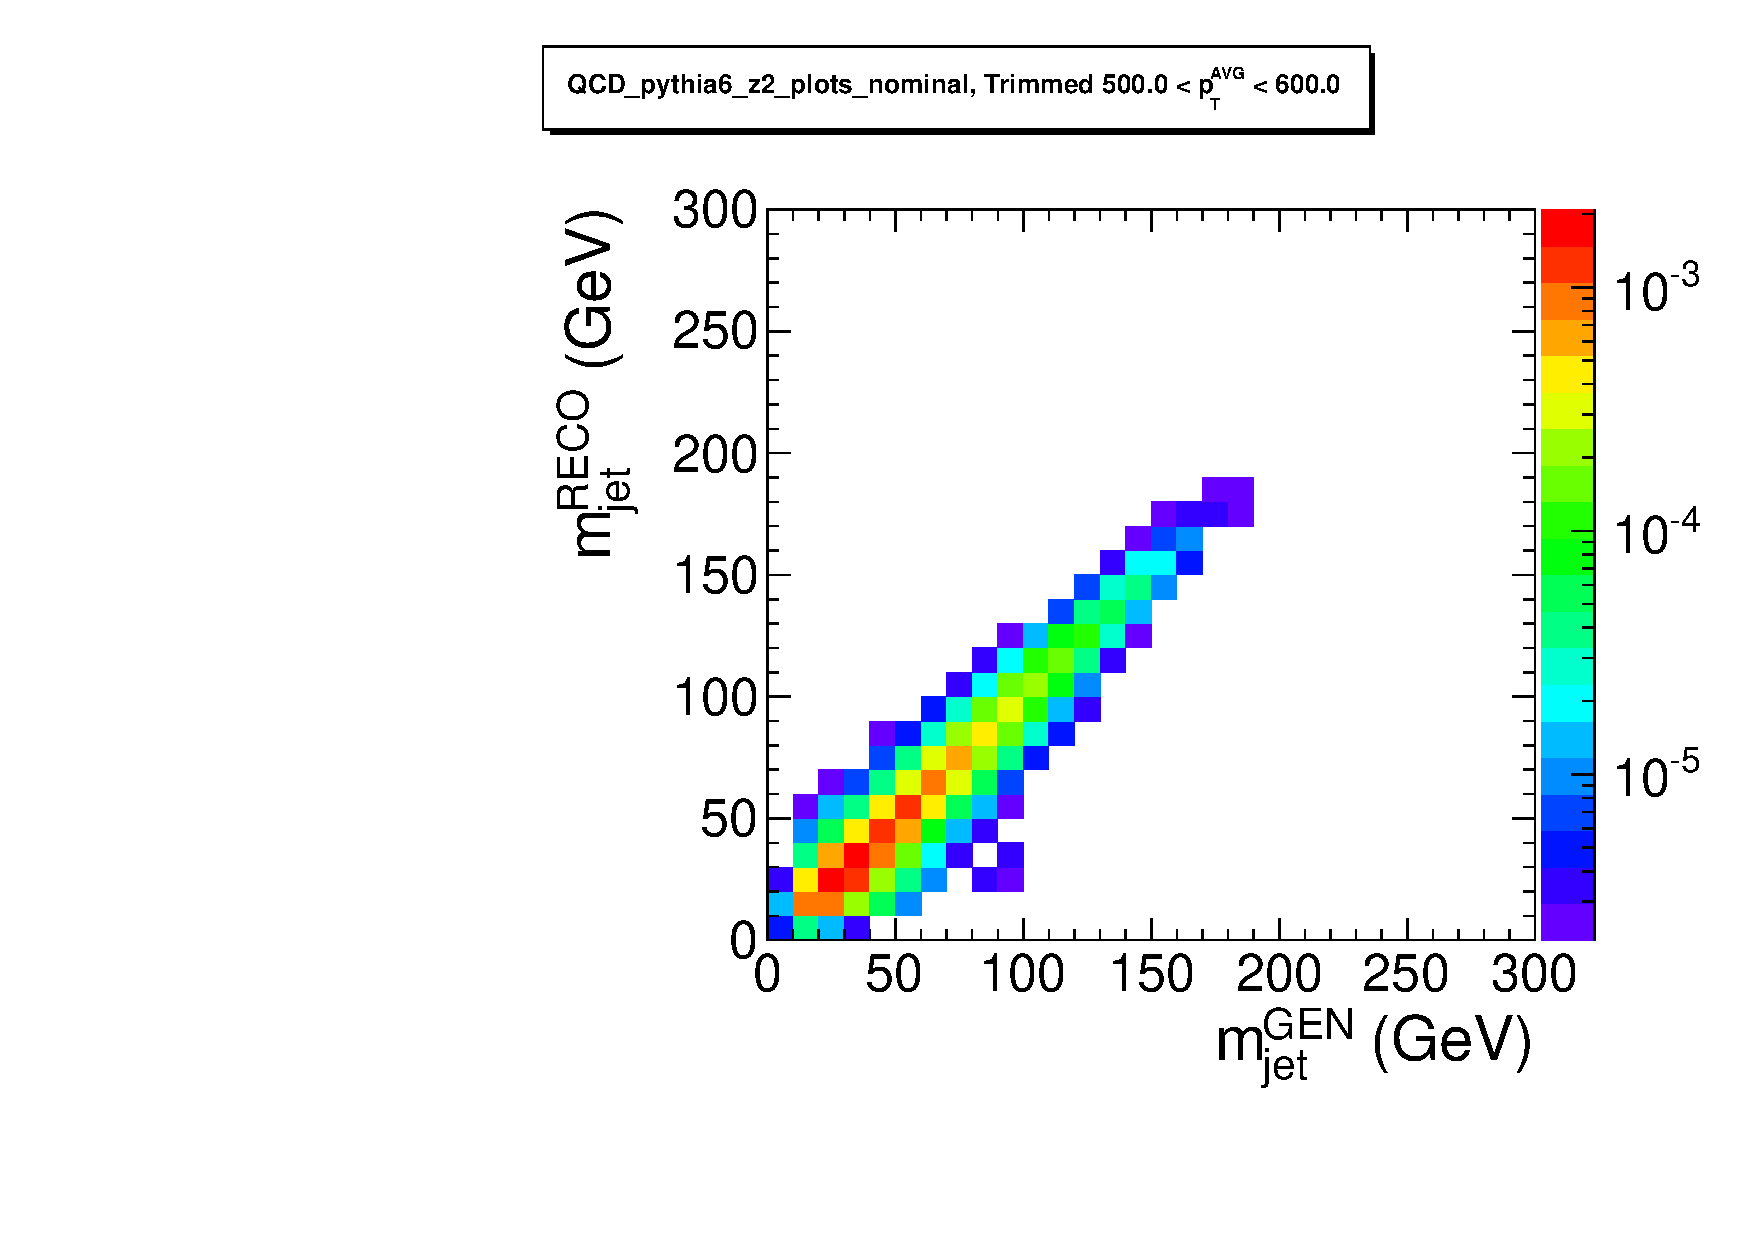
\includegraphics[width=0.3\textwidth]{figs/response_QCD_pythia6_z2_plots_nominal_Trimmed_pt7}}
\subfigure{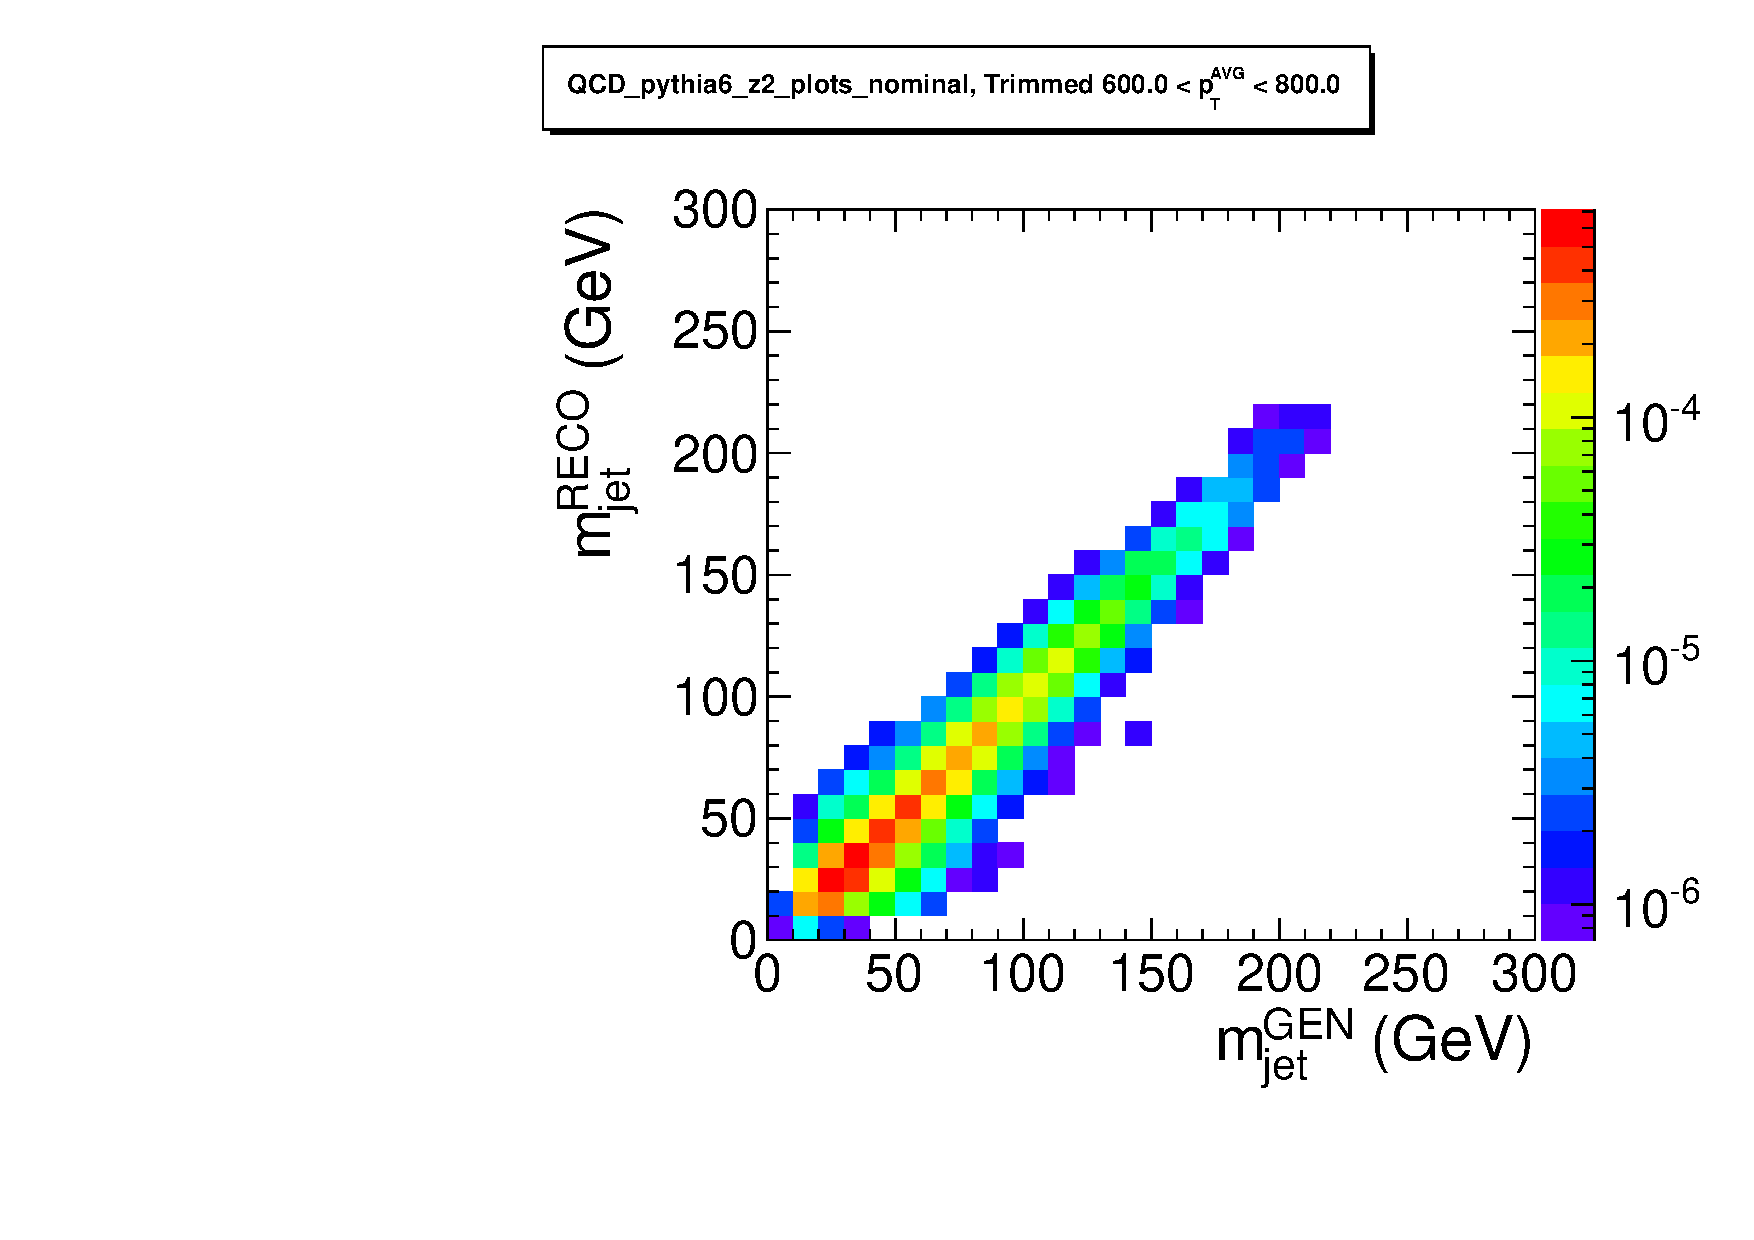
\includegraphics[width=0.3\textwidth]{figs/response_QCD_pythia6_z2_plots_nominal_Trimmed_pt8}}
\subfigure{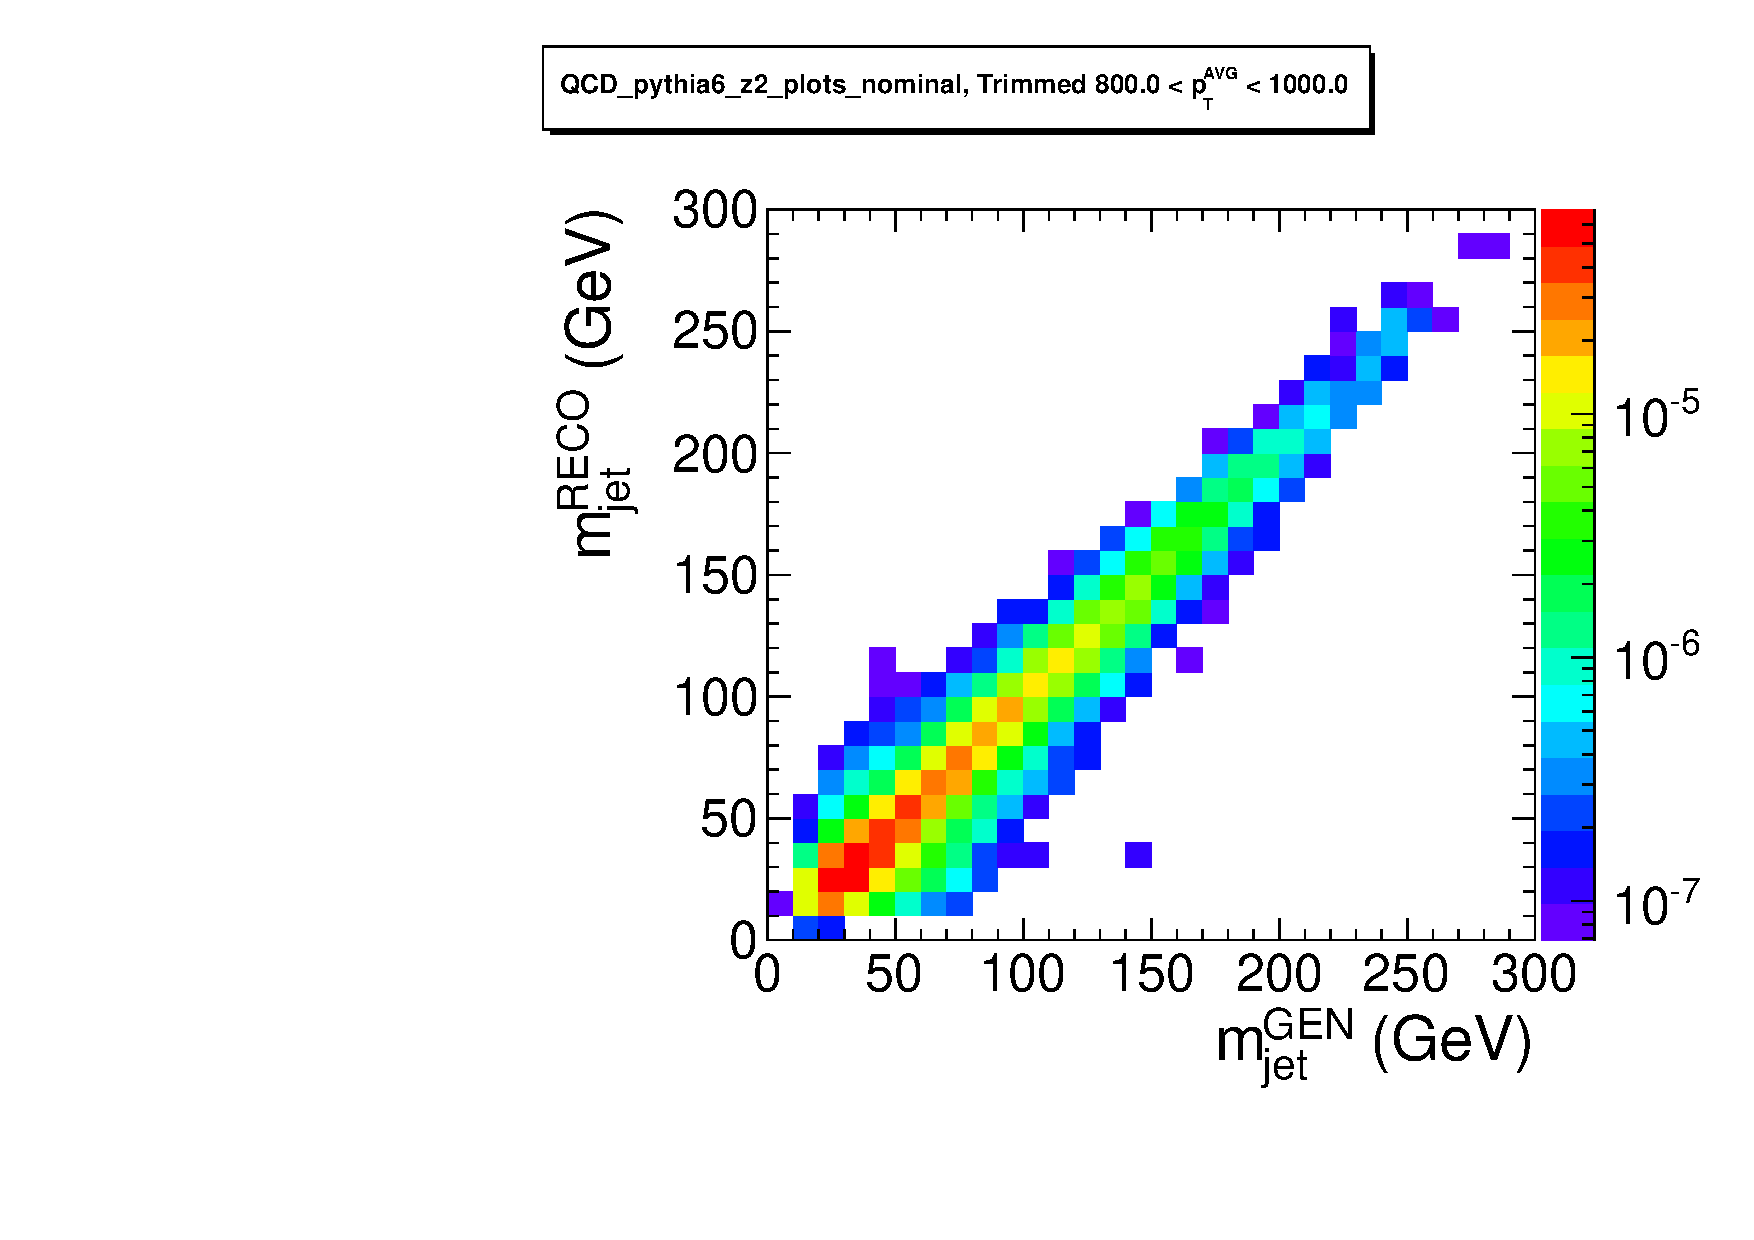
\includegraphics[width=0.3\textwidth]{figs/response_QCD_pythia6_z2_plots_nominal_Trimmed_pt9}}\\
\caption{Response of the jet mass for AK7 Trimmedjets,
for various $\pt^{AVG}$ bins. The true jet mass is shown
on the $x-$axis, and the reconstructed jet mass is shown on the
$y-$axis, using the \PYTHIA generator. 
\label{figs:response_QCD_pythia6_z2_plots_nominal_Trimmed_ptall}}
\end{figure}


\clearpage

\begin{figure}[htbp]
\centering
\subfigure{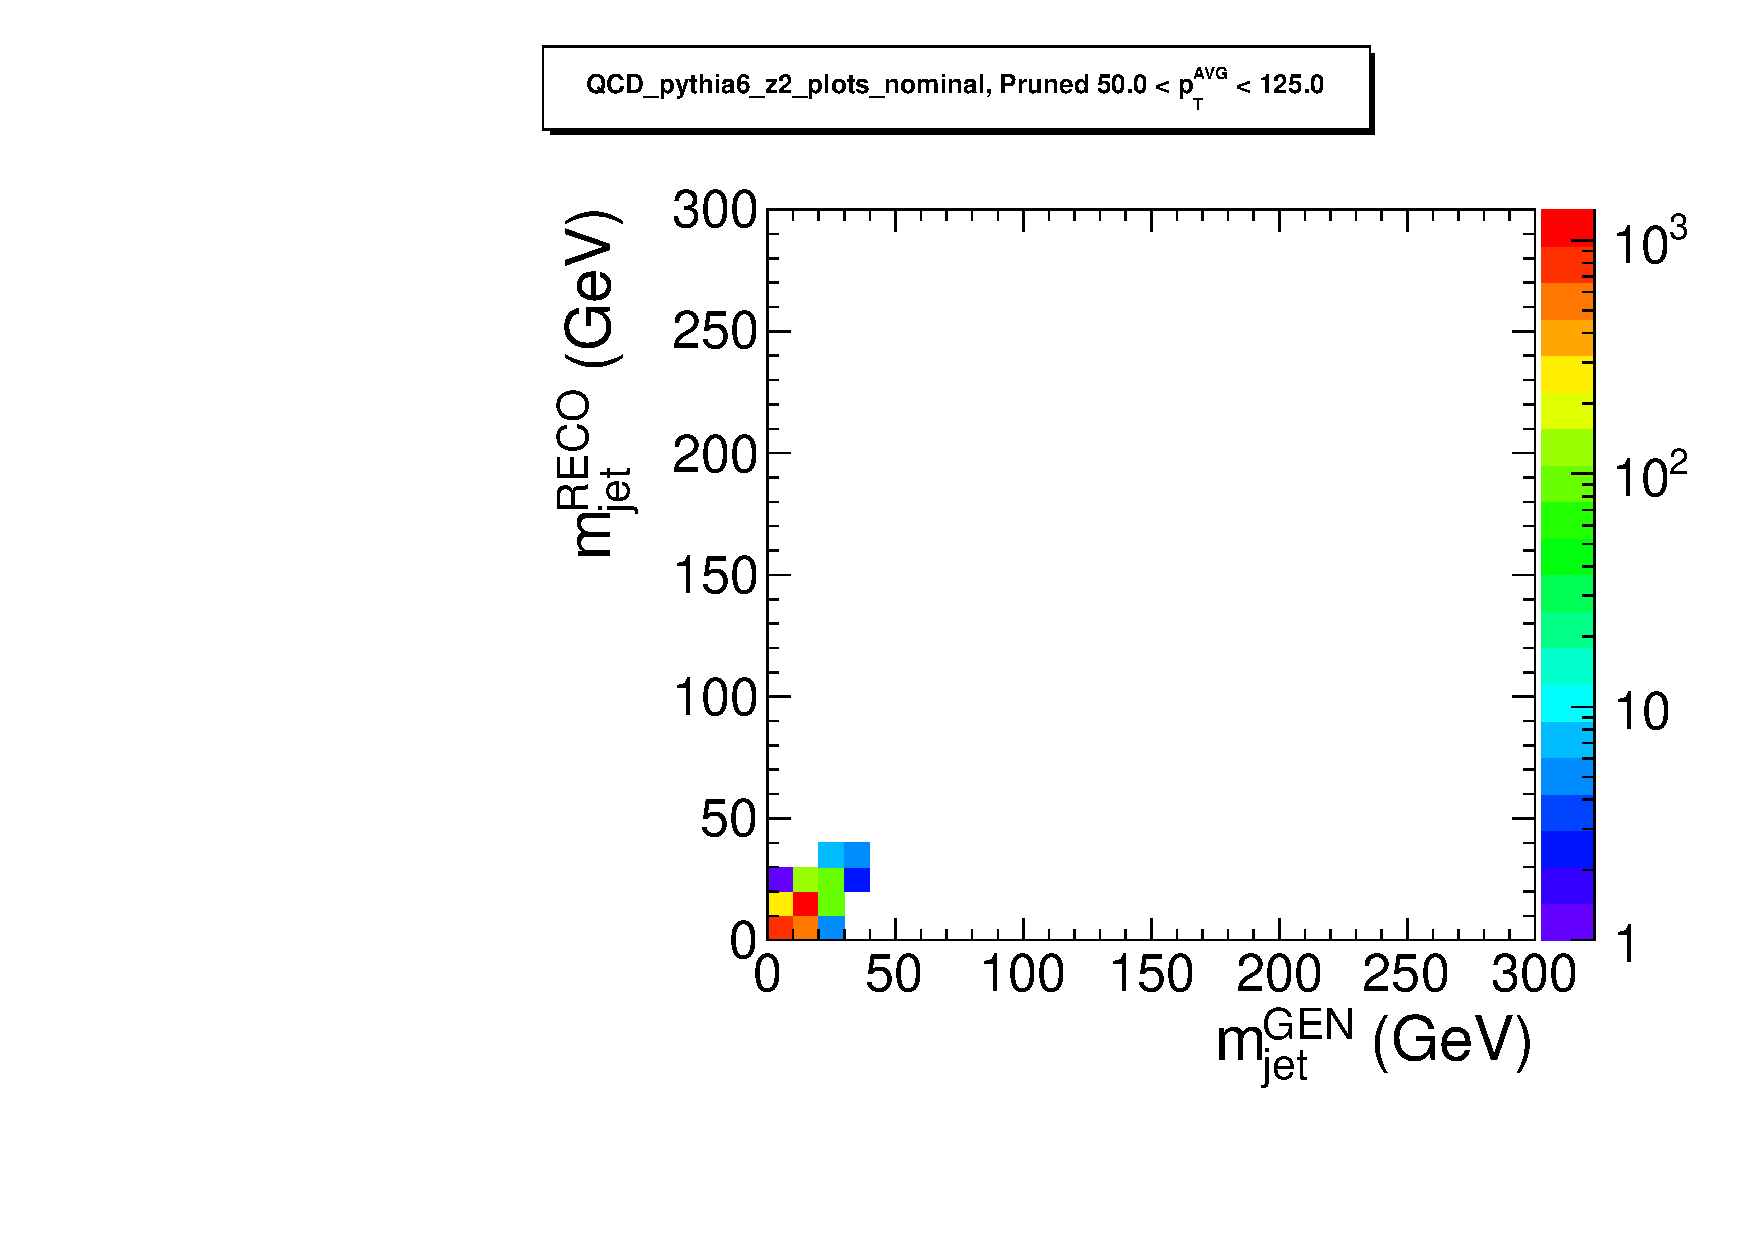
\includegraphics[width=0.3\textwidth]{figs/response_QCD_pythia6_z2_plots_nominal_Pruned_pt1}}
\subfigure{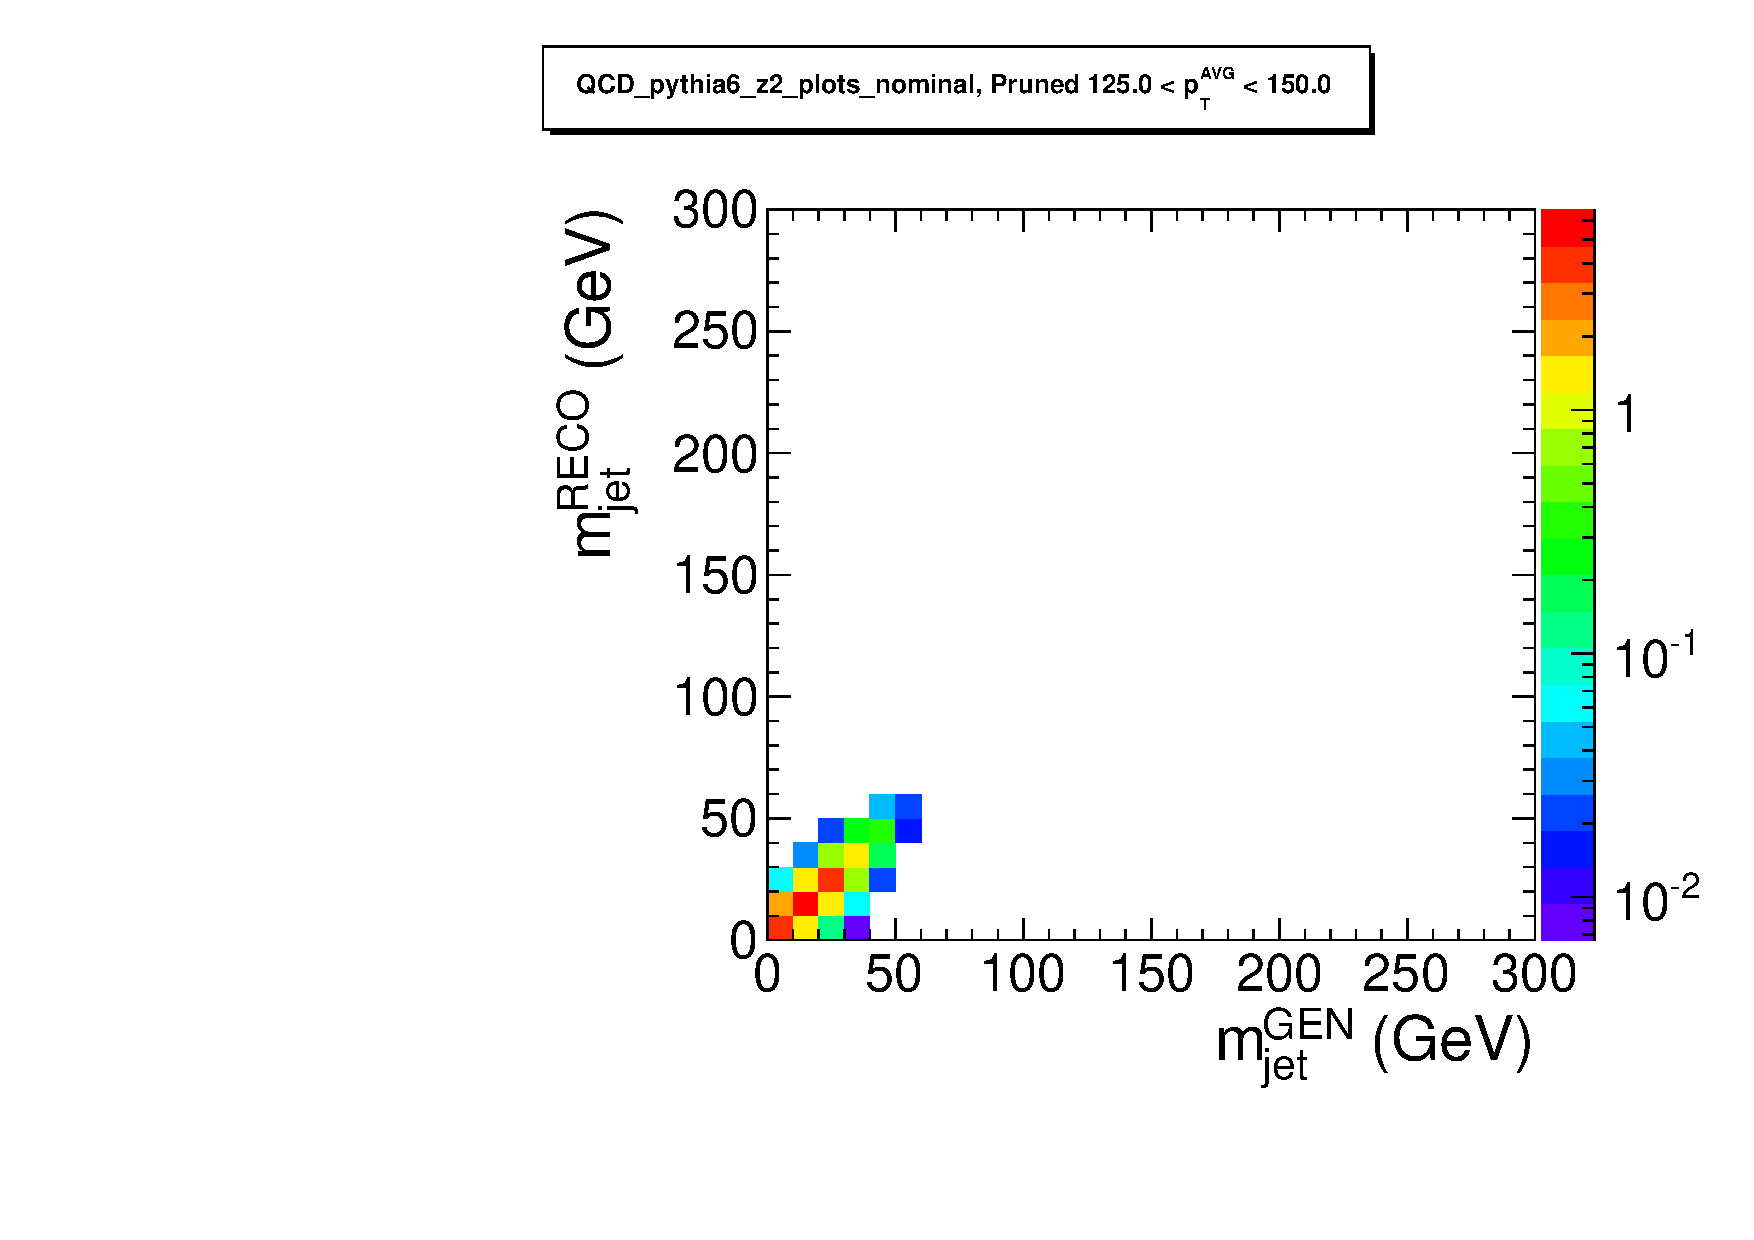
\includegraphics[width=0.3\textwidth]{figs/response_QCD_pythia6_z2_plots_nominal_Pruned_pt2}}
\subfigure{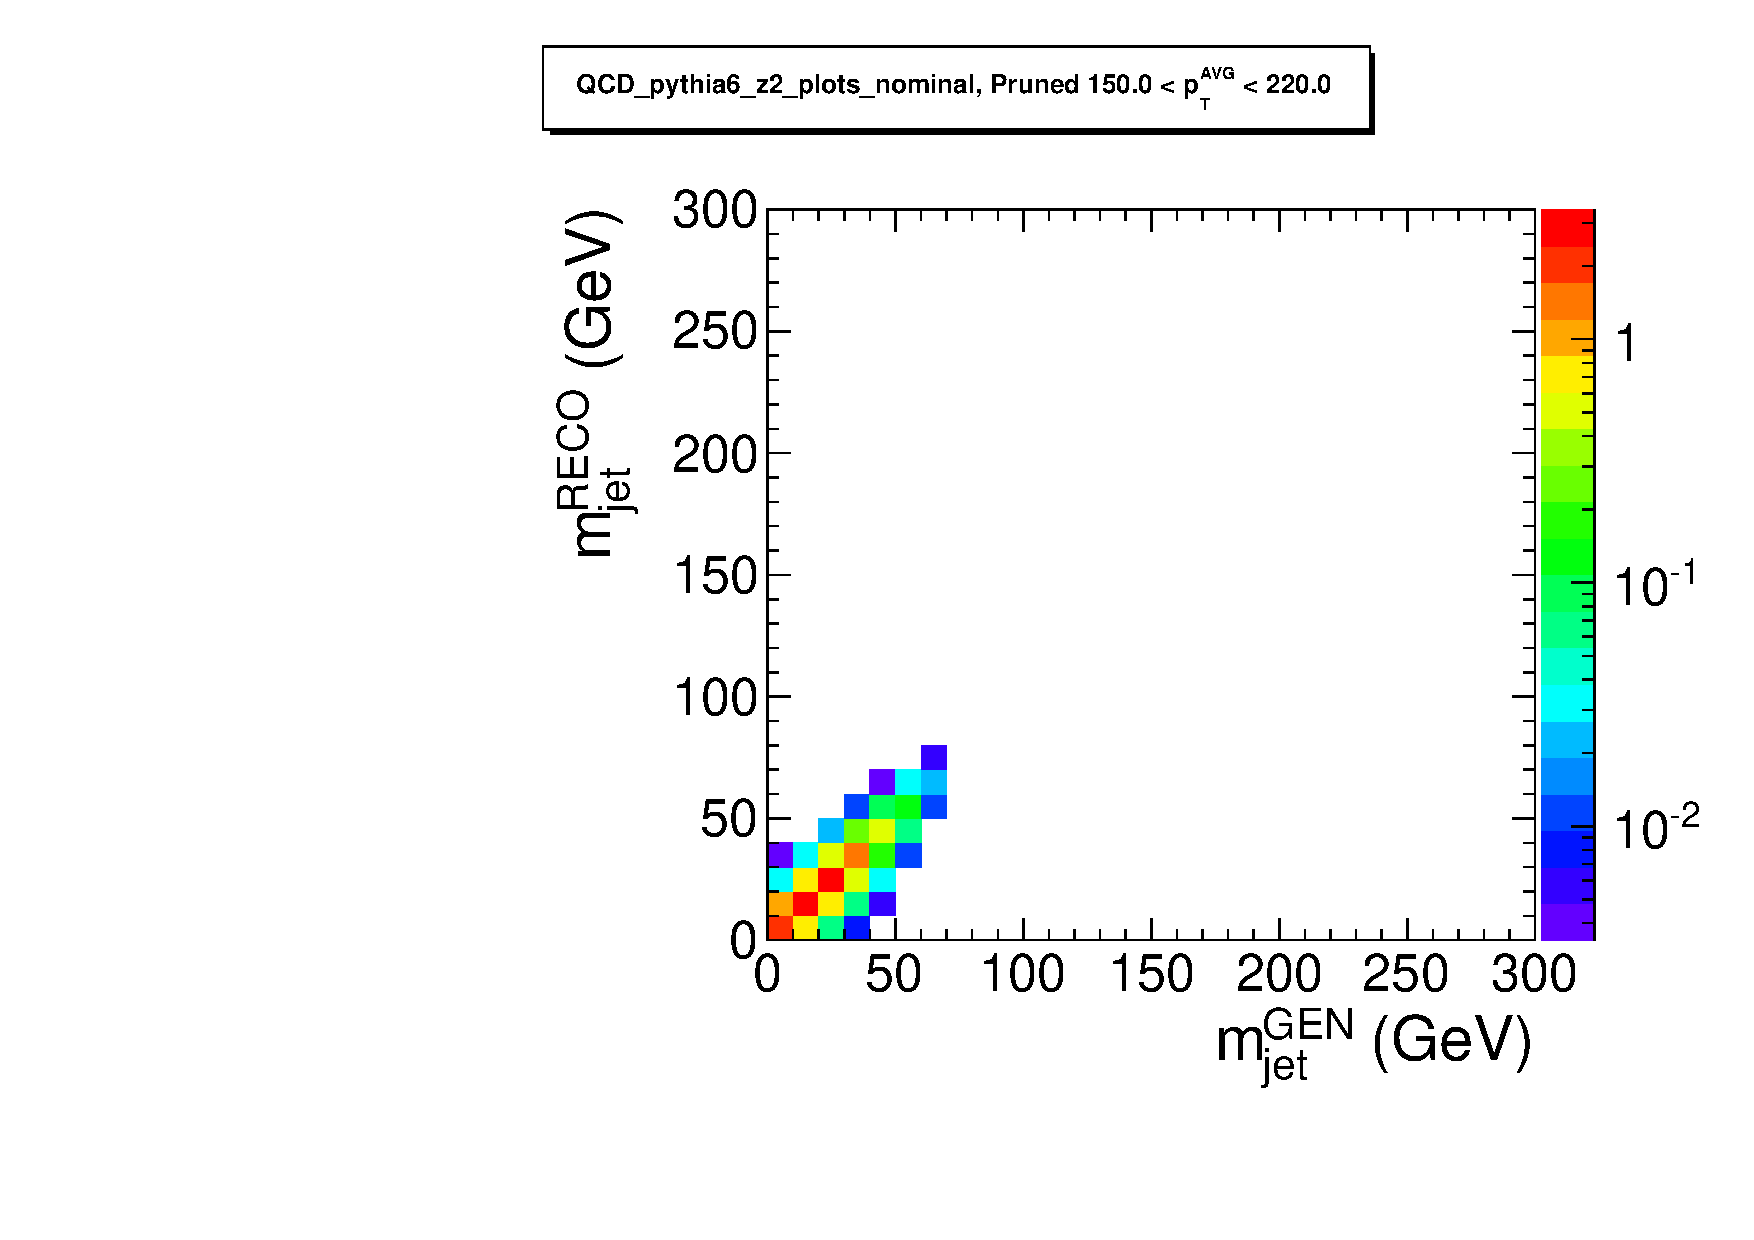
\includegraphics[width=0.3\textwidth]{figs/response_QCD_pythia6_z2_plots_nominal_Pruned_pt3}}\\
\subfigure{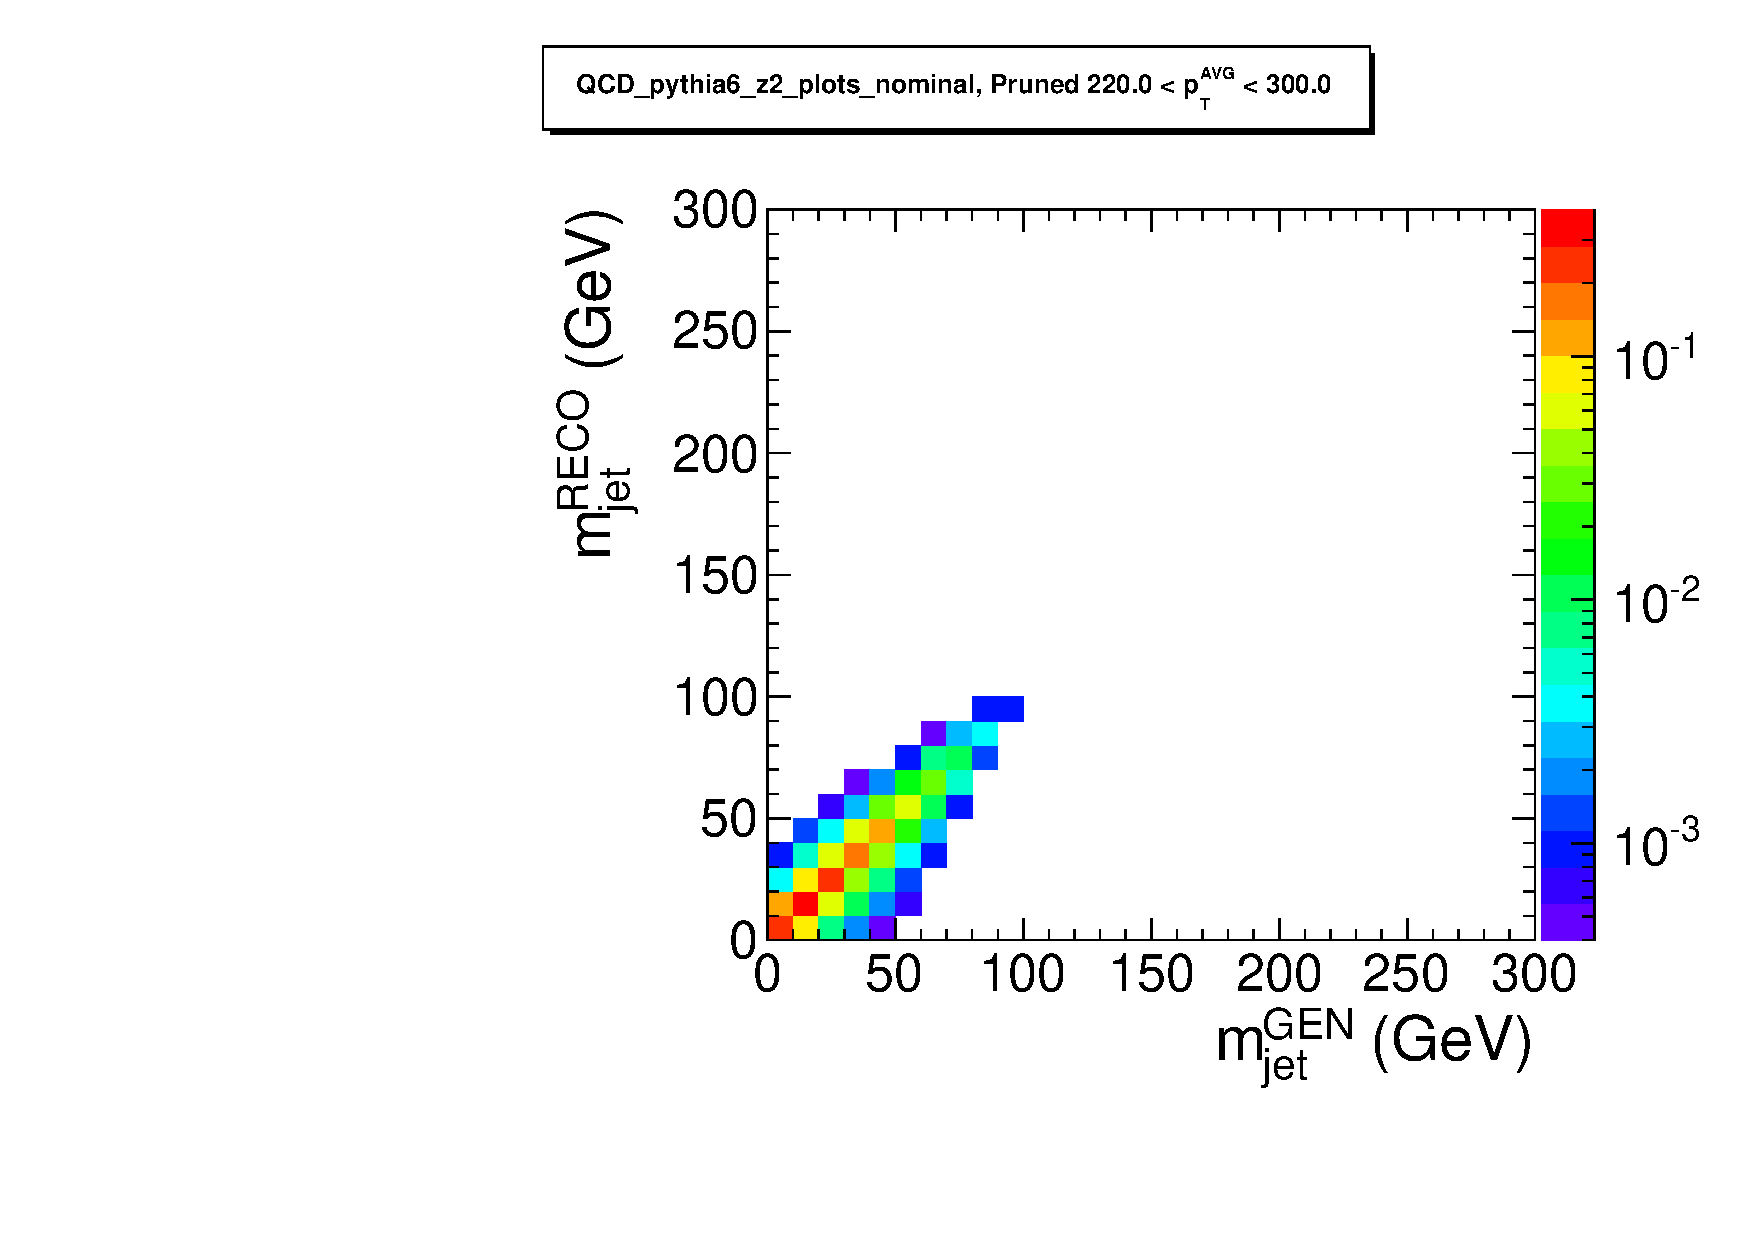
\includegraphics[width=0.3\textwidth]{figs/response_QCD_pythia6_z2_plots_nominal_Pruned_pt4}}
\subfigure{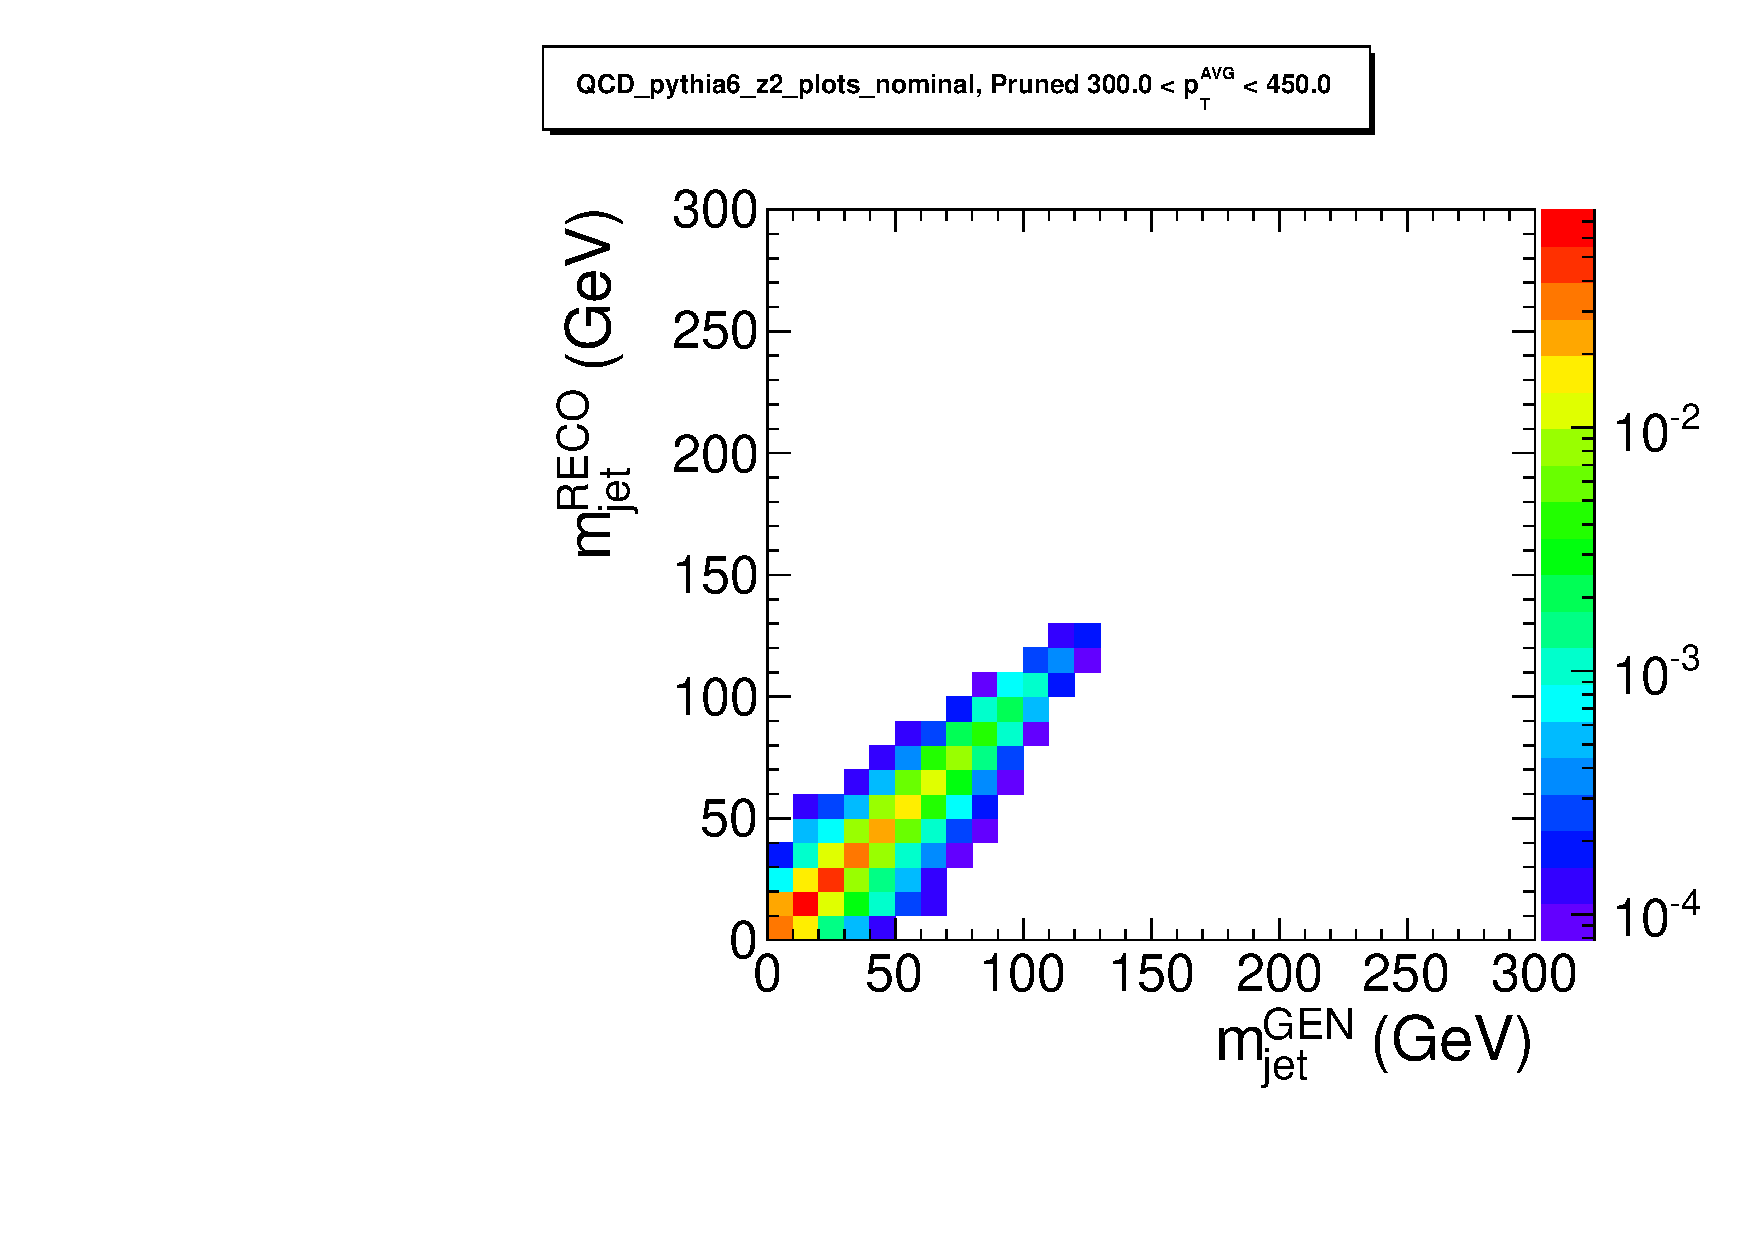
\includegraphics[width=0.3\textwidth]{figs/response_QCD_pythia6_z2_plots_nominal_Pruned_pt5}}
\subfigure{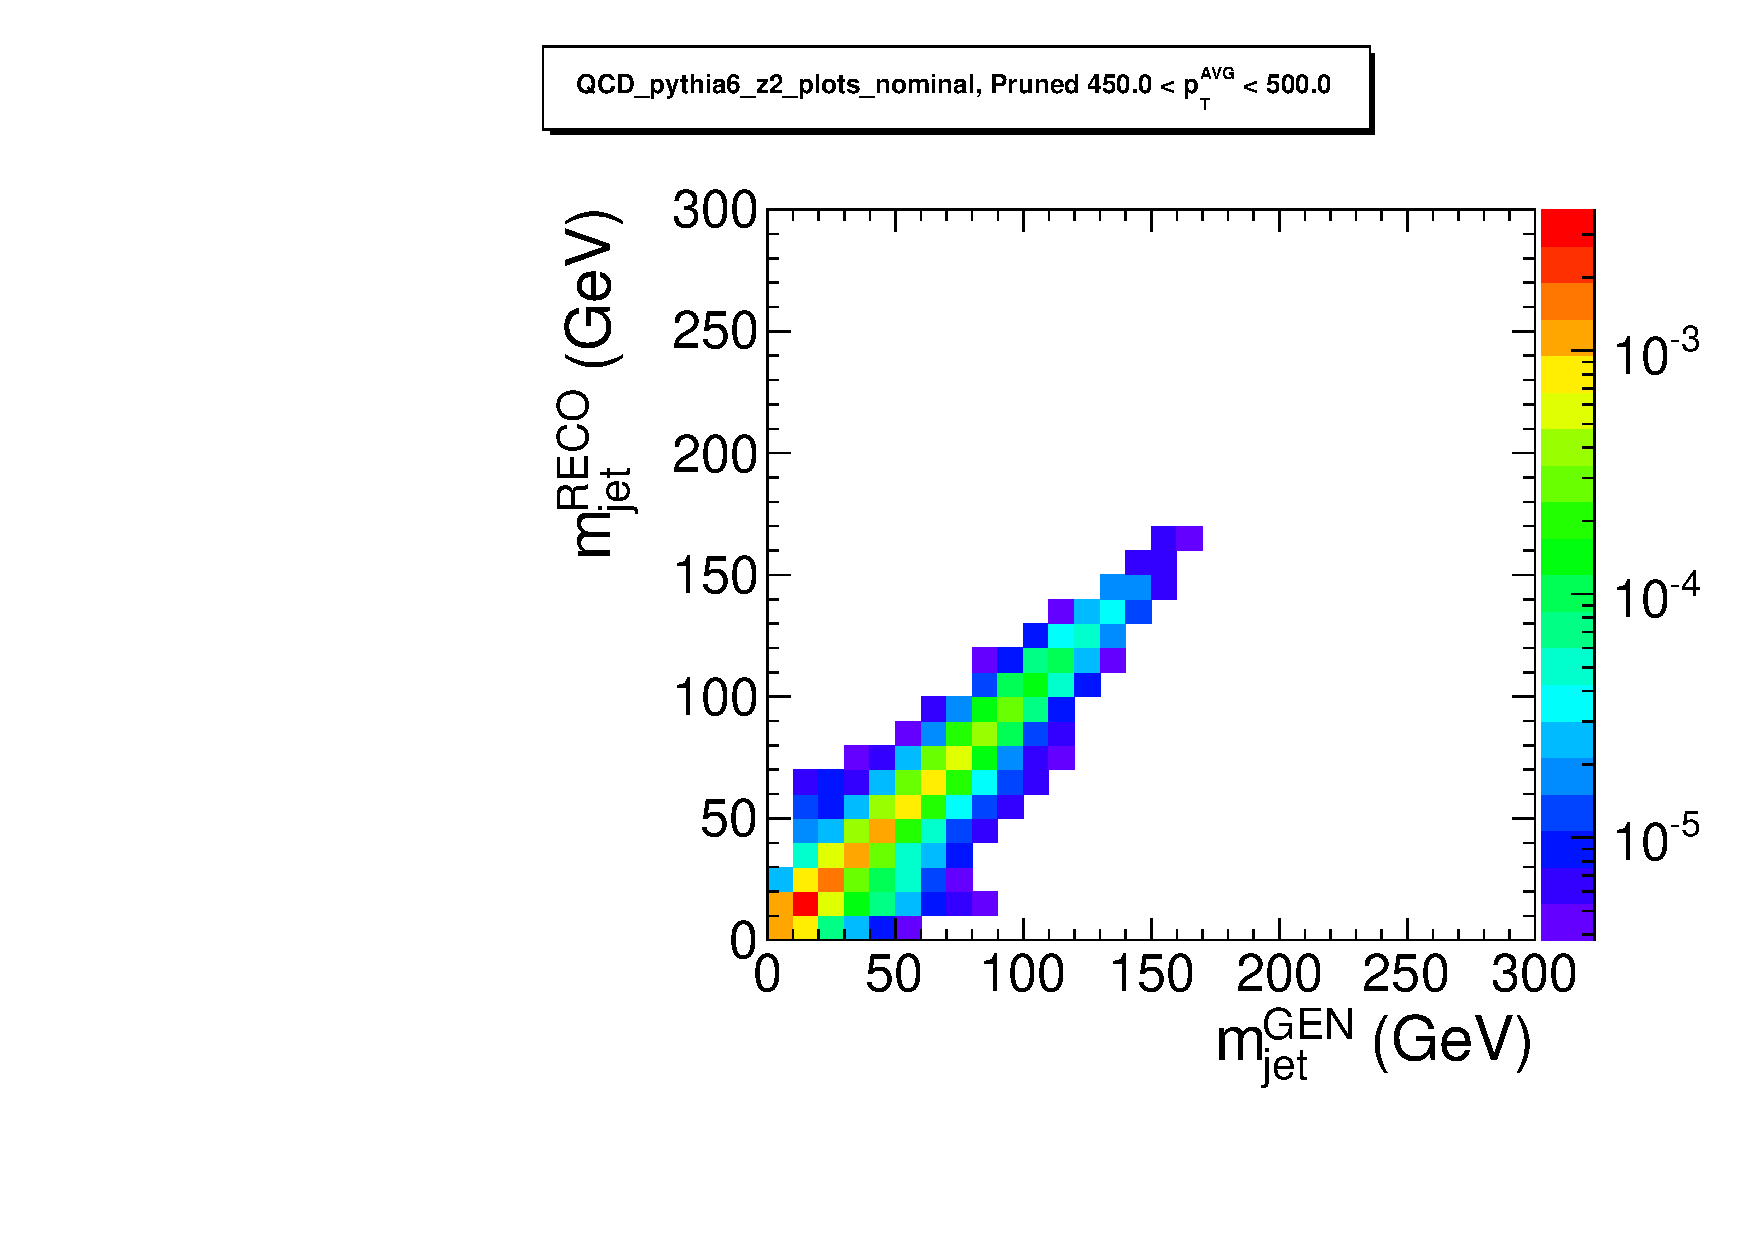
\includegraphics[width=0.3\textwidth]{figs/response_QCD_pythia6_z2_plots_nominal_Pruned_pt6}}\\
\subfigure{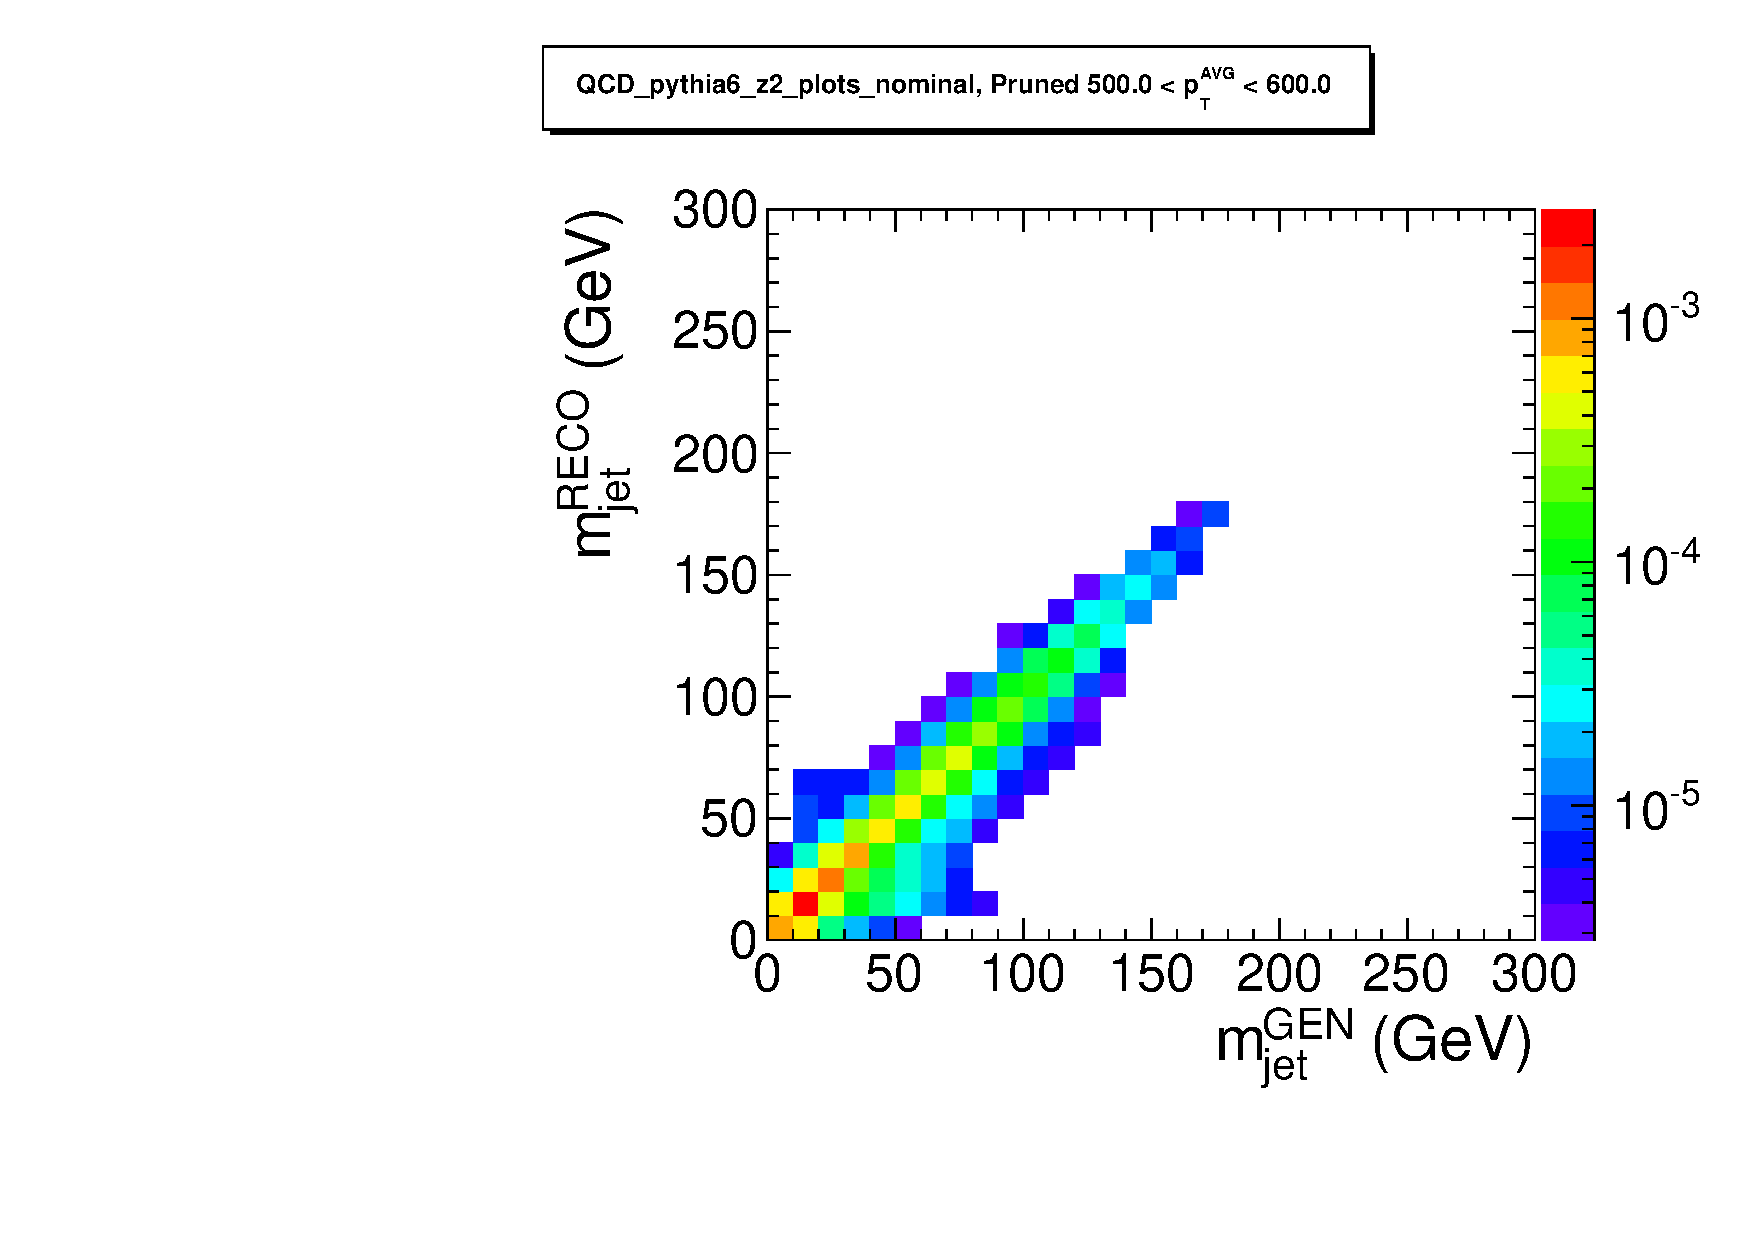
\includegraphics[width=0.3\textwidth]{figs/response_QCD_pythia6_z2_plots_nominal_Pruned_pt7}}
\subfigure{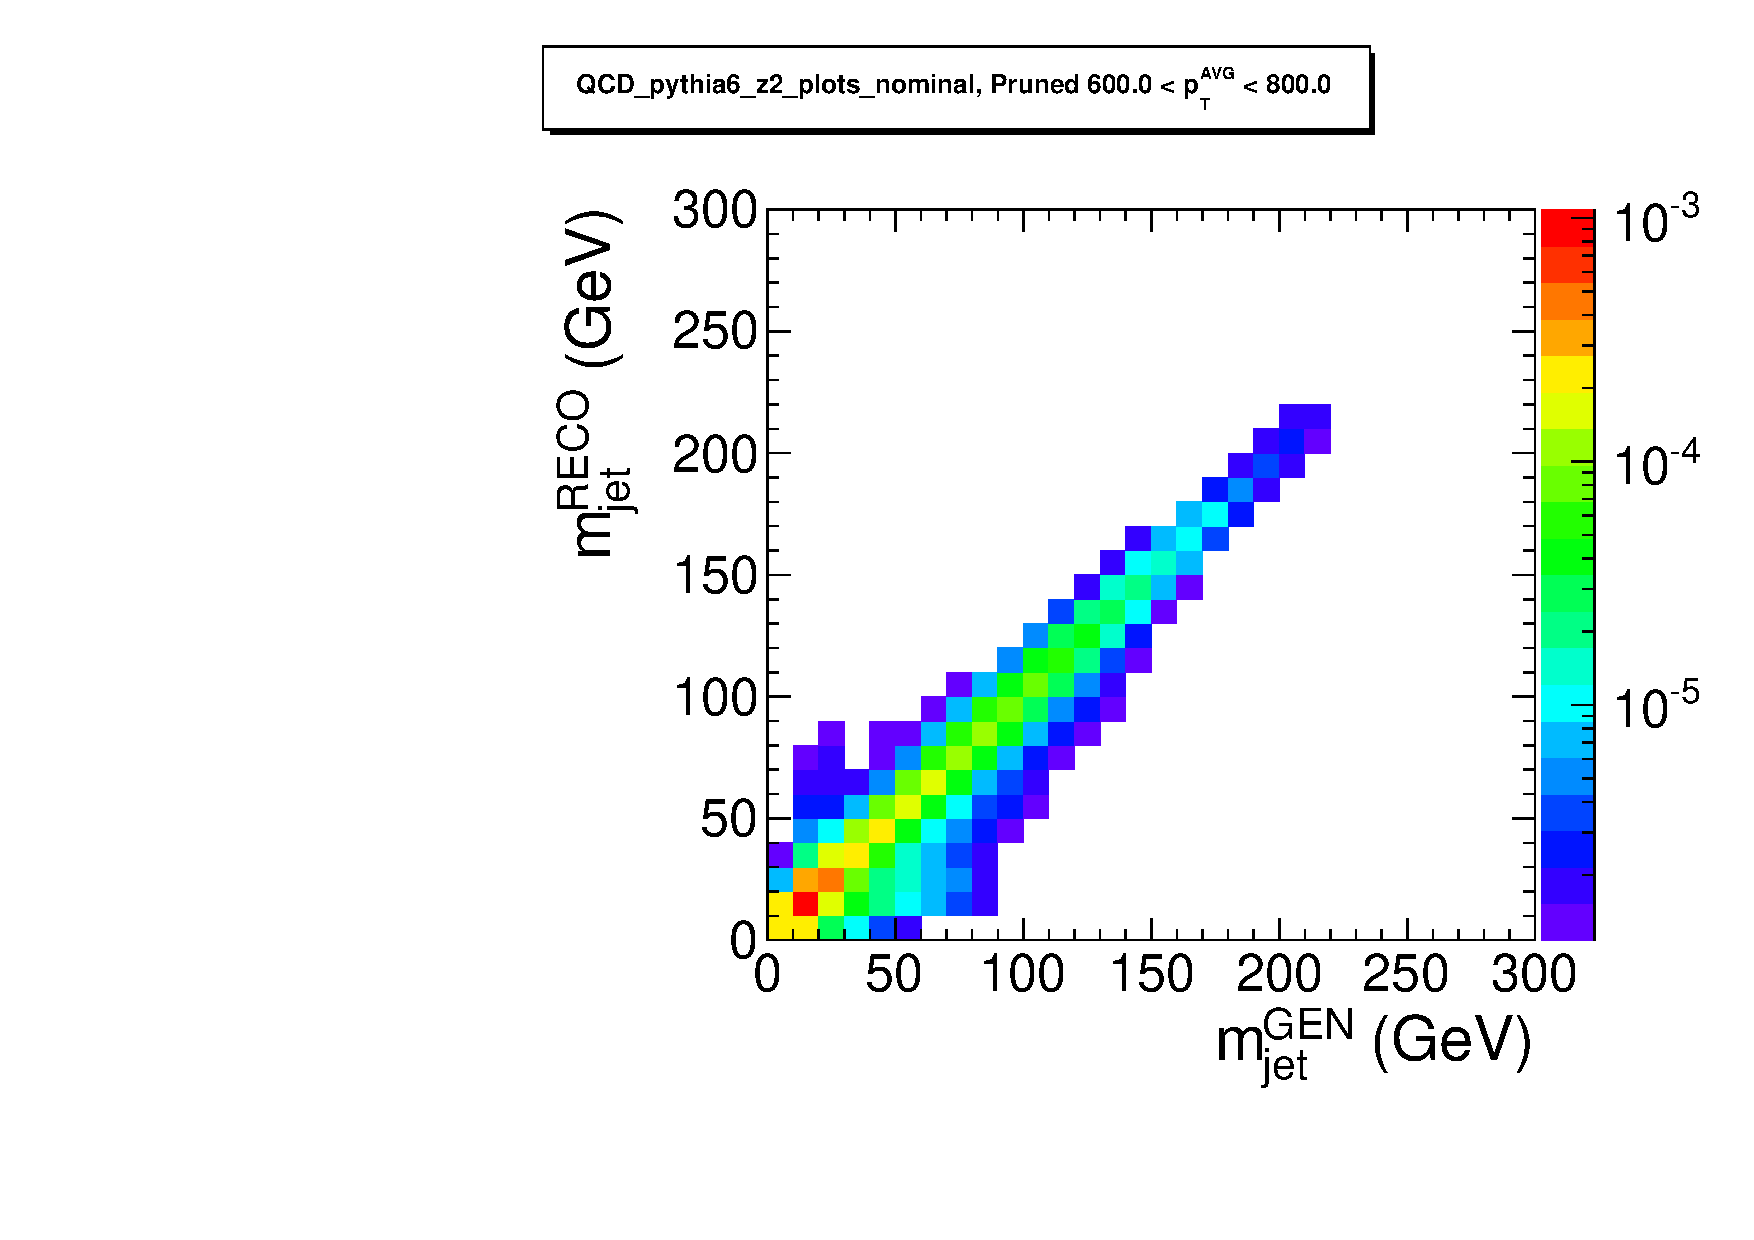
\includegraphics[width=0.3\textwidth]{figs/response_QCD_pythia6_z2_plots_nominal_Pruned_pt8}}
\subfigure{\includegraphics[width=0.3\textwidth]{figs/response_QCD_pythia6_z2_plots_nominal_Pruned_pt9}}\\
\caption{Response of the jet mass for AK7 Prunedjets,
for various $\pt^{AVG}$ bins. The true jet mass is shown
on the $x-$axis, and the reconstructed jet mass is shown on the
$y-$axis, using the \PYTHIA generator. 
\label{figs:response_QCD_pythia6_z2_plots_nominal_Pruned_ptall}}
\end{figure}


\clearpage

\begin{figure}[htbp]
\centering
\subfigure{\includegraphics[width=0.3\textwidth]{figs/response_QCD_pythia8_4c_plots_nominal_pt1}}
\subfigure{\includegraphics[width=0.3\textwidth]{figs/response_QCD_pythia8_4c_plots_nominal_pt2}}
\subfigure{\includegraphics[width=0.3\textwidth]{figs/response_QCD_pythia8_4c_plots_nominal_pt3}}\\
\subfigure{\includegraphics[width=0.3\textwidth]{figs/response_QCD_pythia8_4c_plots_nominal_pt4}}
\subfigure{\includegraphics[width=0.3\textwidth]{figs/response_QCD_pythia8_4c_plots_nominal_pt5}}
\subfigure{\includegraphics[width=0.3\textwidth]{figs/response_QCD_pythia8_4c_plots_nominal_pt6}}\\
\subfigure{\includegraphics[width=0.3\textwidth]{figs/response_QCD_pythia8_4c_plots_nominal_pt7}}
\subfigure{\includegraphics[width=0.3\textwidth]{figs/response_QCD_pythia8_4c_plots_nominal_pt8}}
\subfigure{\includegraphics[width=0.3\textwidth]{figs/response_QCD_pythia8_4c_plots_nominal_pt9}}\\
\caption{Response of the jet mass for AK7 jets,
for various $\pt^{AVG}$ bins. The true jet mass is shown
on the $x-$axis, and the reconstructed jet mass is shown on the
$y-$axis, using the \PYTHIAEIGHT generator. 
\label{figs:response_QCD_pythia8_4c_plots_nominal_ptall}}
\end{figure}


\clearpage

\begin{figure}[htbp]
\centering
\subfigure{\includegraphics[width=0.3\textwidth]{figs/response_QCD_pythia8_4c_plots_nominal_Filtered_pt1}}
\subfigure{\includegraphics[width=0.3\textwidth]{figs/response_QCD_pythia8_4c_plots_nominal_Filtered_pt2}}
\subfigure{\includegraphics[width=0.3\textwidth]{figs/response_QCD_pythia8_4c_plots_nominal_Filtered_pt3}}\\
\subfigure{\includegraphics[width=0.3\textwidth]{figs/response_QCD_pythia8_4c_plots_nominal_Filtered_pt4}}
\subfigure{\includegraphics[width=0.3\textwidth]{figs/response_QCD_pythia8_4c_plots_nominal_Filtered_pt5}}
\subfigure{\includegraphics[width=0.3\textwidth]{figs/response_QCD_pythia8_4c_plots_nominal_Filtered_pt6}}\\
\subfigure{\includegraphics[width=0.3\textwidth]{figs/response_QCD_pythia8_4c_plots_nominal_Filtered_pt7}}
\subfigure{\includegraphics[width=0.3\textwidth]{figs/response_QCD_pythia8_4c_plots_nominal_Filtered_pt8}}
\subfigure{\includegraphics[width=0.3\textwidth]{figs/response_QCD_pythia8_4c_plots_nominal_Filtered_pt9}}\\
\caption{Response of the jet mass for AK7 Filteredjets,
for various $\pt^{AVG}$ bins. The true jet mass is shown
on the $x-$axis, and the reconstructed jet mass is shown on the
$y-$axis, using the \PYTHIAEIGHT generator. 
\label{figs:response_QCD_pythia8_4c_plots_nominal_Filtered_ptall}}
\end{figure}


\clearpage

\begin{figure}[htbp]
\centering
\subfigure{\includegraphics[width=0.3\textwidth]{figs/response_QCD_pythia8_4c_plots_nominal_Trimmed_pt1}}
\subfigure{\includegraphics[width=0.3\textwidth]{figs/response_QCD_pythia8_4c_plots_nominal_Trimmed_pt2}}
\subfigure{\includegraphics[width=0.3\textwidth]{figs/response_QCD_pythia8_4c_plots_nominal_Trimmed_pt3}}\\
\subfigure{\includegraphics[width=0.3\textwidth]{figs/response_QCD_pythia8_4c_plots_nominal_Trimmed_pt4}}
\subfigure{\includegraphics[width=0.3\textwidth]{figs/response_QCD_pythia8_4c_plots_nominal_Trimmed_pt5}}
\subfigure{\includegraphics[width=0.3\textwidth]{figs/response_QCD_pythia8_4c_plots_nominal_Trimmed_pt6}}\\
\subfigure{\includegraphics[width=0.3\textwidth]{figs/response_QCD_pythia8_4c_plots_nominal_Trimmed_pt7}}
\subfigure{\includegraphics[width=0.3\textwidth]{figs/response_QCD_pythia8_4c_plots_nominal_Trimmed_pt8}}
\subfigure{\includegraphics[width=0.3\textwidth]{figs/response_QCD_pythia8_4c_plots_nominal_Trimmed_pt9}}\\
\caption{Response of the jet mass for AK7 Trimmedjets,
for various $\pt^{AVG}$ bins. The true jet mass is shown
on the $x-$axis, and the reconstructed jet mass is shown on the
$y-$axis, using the \PYTHIAEIGHT generator. 
\label{figs:response_QCD_pythia8_4c_plots_nominal_Trimmed_ptall}}
\end{figure}


\clearpage

\begin{figure}[htbp]
\centering
\subfigure{\includegraphics[width=0.3\textwidth]{figs/response_QCD_pythia8_4c_plots_nominal_Pruned_pt1}}
\subfigure{\includegraphics[width=0.3\textwidth]{figs/response_QCD_pythia8_4c_plots_nominal_Pruned_pt2}}
\subfigure{\includegraphics[width=0.3\textwidth]{figs/response_QCD_pythia8_4c_plots_nominal_Pruned_pt3}}\\
\subfigure{\includegraphics[width=0.3\textwidth]{figs/response_QCD_pythia8_4c_plots_nominal_Pruned_pt4}}
\subfigure{\includegraphics[width=0.3\textwidth]{figs/response_QCD_pythia8_4c_plots_nominal_Pruned_pt5}}
\subfigure{\includegraphics[width=0.3\textwidth]{figs/response_QCD_pythia8_4c_plots_nominal_Pruned_pt6}}\\
\subfigure{\includegraphics[width=0.3\textwidth]{figs/response_QCD_pythia8_4c_plots_nominal_Pruned_pt7}}
\subfigure{\includegraphics[width=0.3\textwidth]{figs/response_QCD_pythia8_4c_plots_nominal_Pruned_pt8}}
\subfigure{\includegraphics[width=0.3\textwidth]{figs/response_QCD_pythia8_4c_plots_nominal_Pruned_pt9}}\\
\caption{Response of the jet mass for AK7 Prunedjets,
for various $\pt^{AVG}$ bins. The true jet mass is shown
on the $x-$axis, and the reconstructed jet mass is shown on the
$y-$axis, using the \PYTHIAEIGHT generator. 
\label{figs:response_QCD_pythia8_4c_plots_nominal_Pruned_ptall}}
\end{figure}


\clearpage

\begin{figure}[htbp]
\centering
\subfigure{\includegraphics[width=0.3\textwidth]{figs/response_QCD_herwigpp_23_plots_nominal_pt1}}
\subfigure{\includegraphics[width=0.3\textwidth]{figs/response_QCD_herwigpp_23_plots_nominal_pt2}}
\subfigure{\includegraphics[width=0.3\textwidth]{figs/response_QCD_herwigpp_23_plots_nominal_pt3}}\\
\subfigure{\includegraphics[width=0.3\textwidth]{figs/response_QCD_herwigpp_23_plots_nominal_pt4}}
\subfigure{\includegraphics[width=0.3\textwidth]{figs/response_QCD_herwigpp_23_plots_nominal_pt5}}
\subfigure{\includegraphics[width=0.3\textwidth]{figs/response_QCD_herwigpp_23_plots_nominal_pt6}}\\
\subfigure{\includegraphics[width=0.3\textwidth]{figs/response_QCD_herwigpp_23_plots_nominal_pt7}}
\subfigure{\includegraphics[width=0.3\textwidth]{figs/response_QCD_herwigpp_23_plots_nominal_pt8}}
\subfigure{\includegraphics[width=0.3\textwidth]{figs/response_QCD_herwigpp_23_plots_nominal_pt9}}\\
\caption{Response of the jet mass for AK7 jets,
for various $\pt^{AVG}$ bins. The true jet mass is shown
on the $x-$axis, and the reconstructed jet mass is shown on the
$y-$axis, using the \HERWIG generator. 
\label{figs:response_QCD_herwigpp_23_plots_nominal_ptall}}
\end{figure}


\clearpage

\begin{figure}[htbp]
\centering
\subfigure{\includegraphics[width=0.3\textwidth]{figs/response_QCD_herwigpp_23_plots_nominal_Filtered_pt1}}
\subfigure{\includegraphics[width=0.3\textwidth]{figs/response_QCD_herwigpp_23_plots_nominal_Filtered_pt2}}
\subfigure{\includegraphics[width=0.3\textwidth]{figs/response_QCD_herwigpp_23_plots_nominal_Filtered_pt3}}\\
\subfigure{\includegraphics[width=0.3\textwidth]{figs/response_QCD_herwigpp_23_plots_nominal_Filtered_pt4}}
\subfigure{\includegraphics[width=0.3\textwidth]{figs/response_QCD_herwigpp_23_plots_nominal_Filtered_pt5}}
\subfigure{\includegraphics[width=0.3\textwidth]{figs/response_QCD_herwigpp_23_plots_nominal_Filtered_pt6}}\\
\subfigure{\includegraphics[width=0.3\textwidth]{figs/response_QCD_herwigpp_23_plots_nominal_Filtered_pt7}}
\subfigure{\includegraphics[width=0.3\textwidth]{figs/response_QCD_herwigpp_23_plots_nominal_Filtered_pt8}}
\subfigure{\includegraphics[width=0.3\textwidth]{figs/response_QCD_herwigpp_23_plots_nominal_Filtered_pt9}}\\
\caption{Response of the jet mass for AK7 Filteredjets,
for various $\pt^{AVG}$ bins. The true jet mass is shown
on the $x-$axis, and the reconstructed jet mass is shown on the
$y-$axis, using the \HERWIG generator. 
\label{figs:response_QCD_herwigpp_23_plots_nominal_Filtered_ptall}}
\end{figure}


\clearpage

\begin{figure}[htbp]
\centering
\subfigure{\includegraphics[width=0.3\textwidth]{figs/response_QCD_herwigpp_23_plots_nominal_Trimmed_pt1}}
\subfigure{\includegraphics[width=0.3\textwidth]{figs/response_QCD_herwigpp_23_plots_nominal_Trimmed_pt2}}
\subfigure{\includegraphics[width=0.3\textwidth]{figs/response_QCD_herwigpp_23_plots_nominal_Trimmed_pt3}}\\
\subfigure{\includegraphics[width=0.3\textwidth]{figs/response_QCD_herwigpp_23_plots_nominal_Trimmed_pt4}}
\subfigure{\includegraphics[width=0.3\textwidth]{figs/response_QCD_herwigpp_23_plots_nominal_Trimmed_pt5}}
\subfigure{\includegraphics[width=0.3\textwidth]{figs/response_QCD_herwigpp_23_plots_nominal_Trimmed_pt6}}\\
\subfigure{\includegraphics[width=0.3\textwidth]{figs/response_QCD_herwigpp_23_plots_nominal_Trimmed_pt7}}
\subfigure{\includegraphics[width=0.3\textwidth]{figs/response_QCD_herwigpp_23_plots_nominal_Trimmed_pt8}}
\subfigure{\includegraphics[width=0.3\textwidth]{figs/response_QCD_herwigpp_23_plots_nominal_Trimmed_pt9}}\\
\caption{Response of the jet mass for AK7 Trimmedjets,
for various $\pt^{AVG}$ bins. The true jet mass is shown
on the $x-$axis, and the reconstructed jet mass is shown on the
$y-$axis, using the \HERWIG generator. 
\label{figs:response_QCD_herwigpp_23_plots_nominal_Trimmed_ptall}}
\end{figure}


\clearpage

\begin{figure}[htbp]
\centering
\subfigure{\includegraphics[width=0.3\textwidth]{figs/response_QCD_herwigpp_23_plots_nominal_Pruned_pt1}}
\subfigure{\includegraphics[width=0.3\textwidth]{figs/response_QCD_herwigpp_23_plots_nominal_Pruned_pt2}}
\subfigure{\includegraphics[width=0.3\textwidth]{figs/response_QCD_herwigpp_23_plots_nominal_Pruned_pt3}}\\
\subfigure{\includegraphics[width=0.3\textwidth]{figs/response_QCD_herwigpp_23_plots_nominal_Pruned_pt4}}
\subfigure{\includegraphics[width=0.3\textwidth]{figs/response_QCD_herwigpp_23_plots_nominal_Pruned_pt5}}
\subfigure{\includegraphics[width=0.3\textwidth]{figs/response_QCD_herwigpp_23_plots_nominal_Pruned_pt6}}\\
\subfigure{\includegraphics[width=0.3\textwidth]{figs/response_QCD_herwigpp_23_plots_nominal_Pruned_pt7}}
\subfigure{\includegraphics[width=0.3\textwidth]{figs/response_QCD_herwigpp_23_plots_nominal_Pruned_pt8}}
\subfigure{\includegraphics[width=0.3\textwidth]{figs/response_QCD_herwigpp_23_plots_nominal_Pruned_pt9}}\\
\caption{Response of the jet mass for AK7 Prunedjets,
for various $\pt^{AVG}$ bins. The true jet mass is shown
on the $x-$axis, and the reconstructed jet mass is shown on the
$y-$axis, using the \HERWIG generator. 
\label{figs:response_QCD_herwigpp_23_plots_nominal_Pruned_ptall}}
\end{figure}


\clearpage


\clearpage

\subsection{Closure test}

\label{sec:closure}

The unfolding procedure we have used makes an assumption that
the dijet events that we are using are the same at the detector
level and the generator level. Furthermore, the jet algorithm
itself is an arbitrary designation of the event, and what to
call a ``jet'' depends on the energy scale of the process.
For these reasons, the assumed dijet topology as described
above may not correspond to the true topology of the event.
Trijet events (and quadjet, etc) can pollute the dijet
events, even with a veto on extra jet activity. This is 
particularly problematic at lower $\pt$. Hence, a critical test
is the closure of our unfolding procedure. That is,
the MC is taken as both the input to the response matrix,
and as simulated ``data'', and compared to the MC true
distribution at the generator level. Any discrepancy here
is a problem with the assumption of the dijet topology.

Figures~\ref{figs:unfoldedMeasurementDijets_1_closuretest}-
\ref{figs:unfoldedMeasurementDijets_9_closuretest}
show the closure test for the various $\pt^{AVG}$ bins
in the sample. Here, the \PYTHIA true distributions
are compared against the unfolded \PYTHIA MC distributions,
using the unfolding matrix derived from \PYTHIA. For perfect
closure, all of the bins will be at unity. 

There are some residual biases that are present for the 
lower ${\pt}^{AVG}$ bins. These are explicitly corrected
in the unfolded distributions, and the correction is
taken as a systematic uncertainty. 

\begin{figure}[htbp]
\centering
\includegraphics[width=0.95\textwidth]{figs/unfoldedMeasurementDijets_1_closuretest}
\caption{Closure test of the unfolding procedure of the jet mass for AK7 jets,
for $50.0 < \pt^{AVG} < 125.0$ \GeVc. The unfolded MC distribution is shown in black points.
The true MC distribution is shown in solid black. For perfect closure, the black points would
lie exactly on the solid black line.  
\label{figs:unfoldedMeasurementDijets_1_closuretest}}
\end{figure}



\begin{figure}[htbp]
\centering
\includegraphics[width=0.95\textwidth]{figs/unfoldedMeasurementDijets_2_closuretest}
\caption{Closure test of the unfolding procedure of the jet mass for AK7 jets,
for $125.0 < \pt^{AVG} < 150.0$ \GeVc. The unfolded MC distribution is shown in black points.
The true MC distribution is shown in solid black. For perfect closure, the black points would
lie exactly on the solid black line.  
\label{figs:unfoldedMeasurementDijets_2_closuretest}}
\end{figure}



\begin{figure}[htbp]
\centering
\includegraphics[width=0.95\textwidth]{figs/unfoldedMeasurementDijets_3_closuretest}
\caption{Closure test of the unfolding procedure of the jet mass for AK7 jets,
for $150.0 < \pt^{AVG} < 220.0$ \GeVc. The unfolded MC distribution is shown in black points.
The true MC distribution is shown in solid black. For perfect closure, the black points would
lie exactly on the solid black line.  
\label{figs:unfoldedMeasurementDijets_3_closuretest}}
\end{figure}



\begin{figure}[htbp]
\centering
\includegraphics[width=0.95\textwidth]{figs/unfoldedMeasurementDijets_4_closuretest}
\caption{Closure test of the unfolding procedure of the jet mass for AK7 jets,
for $220.0 < \pt^{AVG} < 300.0$ \GeVc. The unfolded MC distribution is shown in black points.
The true MC distribution is shown in solid black. For perfect closure, the black points would
lie exactly on the solid black line.  
\label{figs:unfoldedMeasurementDijets_4_closuretest}}
\end{figure}



\begin{figure}[htbp]
\centering
\includegraphics[width=0.95\textwidth]{figs/unfoldedMeasurementDijets_5_closuretest}
\caption{Closure test of the unfolding procedure of the jet mass for AK7 jets,
for $300.0 < \pt^{AVG} < 450.0$ \GeVc. The unfolded MC distribution is shown in black points.
The true MC distribution is shown in solid black. For perfect closure, the black points would
lie exactly on the solid black line.  
\label{figs:unfoldedMeasurementDijets_5_closuretest}}
\end{figure}



\begin{figure}[htbp]
\centering
\includegraphics[width=0.95\textwidth]{figs/unfoldedMeasurementDijets_6_closuretest}
\caption{Closure test of the unfolding procedure of the jet mass for AK7 jets,
for $450.0 < \pt^{AVG} < 500.0$ \GeVc. The unfolded MC distribution is shown in black points.
The true MC distribution is shown in solid black. For perfect closure, the black points would
lie exactly on the solid black line.  
\label{figs:unfoldedMeasurementDijets_6_closuretest}}
\end{figure}



\begin{figure}[htbp]
\centering
\includegraphics[width=0.95\textwidth]{figs/unfoldedMeasurementDijets_7_closuretest}
\caption{Closure test of the unfolding procedure of the jet mass for AK7 jets,
for $500.0 < \pt^{AVG} < 600.0$ \GeVc. The unfolded MC distribution is shown in black points.
The true MC distribution is shown in solid black. For perfect closure, the black points would
lie exactly on the solid black line.  
\label{figs:unfoldedMeasurementDijets_7_closuretest}}
\end{figure}



\begin{figure}[htbp]
\centering
\includegraphics[width=0.95\textwidth]{figs/unfoldedMeasurementDijets_8_closuretest}
\caption{Closure test of the unfolding procedure of the jet mass for AK7 jets,
for $600.0 < \pt^{AVG} < 800.0$ \GeVc. The unfolded MC distribution is shown in black points.
The true MC distribution is shown in solid black. For perfect closure, the black points would
lie exactly on the solid black line.  
\label{figs:unfoldedMeasurementDijets_8_closuretest}}
\end{figure}



\begin{figure}[htbp]
\centering
\includegraphics[width=0.95\textwidth]{figs/unfoldedMeasurementDijets_9_closuretest}
\caption{Closure test of the unfolding procedure of the jet mass for AK7 jets,
for $800.0 < \pt^{AVG} < 1000.0$ \GeVc. The unfolded MC distribution is shown in black points.
The true MC distribution is shown in solid black. For perfect closure, the black points would
lie exactly on the solid black line.  
\label{figs:unfoldedMeasurementDijets_9_closuretest}}
\end{figure}



\begin{figure}[htbp]
\centering
\includegraphics[width=0.95\textwidth]{figs/unfoldedMeasurementDijets_10_closuretest}
\caption{Closure test of the unfolding procedure of the jet mass for AK7 jets,
for $1000.0 < \pt^{AVG} < 1500.0$ \GeVc. The unfolded MC distribution is shown in black points.
The true MC distribution is shown in solid black. For perfect closure, the black points would
lie exactly on the solid black line.  
\label{figs:unfoldedMeasurementDijets_10_closuretest}}
\end{figure}

\clearpage



\clearpage

\section{Systematic uncertainties}
\section{Other systematics sources}
\label{sec:systematics}
% ---- ---- ---- ---- ---- ---- ---- ---- ---- ---- ---- ---- ---- ---- ---- ---- ---- ---- ---- ---- ---- ---- ----


\subsection{Jet energy scale}
% .... .... .... .... .... .... .... .... .... .... .... .... .... .... .... .... .... .... .... .... .... .... ....


To evaluate the uncertainty due to jet energy scale in events with the
topology of this analysis, we reconstruct the hadronic W candidate
from an almost pure top data control sample.  A semileptonic top
sample is a good proxy for signal for the purposes of this study,
since the top quark pairs are produced by gluon fusion and decay to
two W bosons. These semileptonic top events are selected by requiring
exactly four jets in the event, out of which two are b-tagged and the
other two are anti-btagged. The hadronic W candidates are formed from
two anti-btagged jets.  The invariant mass of the hadronic W
candidates in the combined channels is shown in
Figure~\ref{fig:topw:muel}, for data and Monte Carlo, together with a
gaussian fit on the peak of each distribution.  The relative
difference between the gaussian means in data and Monte Carlo is used
as jet energy scale uncertainty, and propagated through the template
fits in the backgrounds, as well as to the signal shapes in the limit
setting. These results for 2012 are consistent with those found for
2011, when the typical effect was found to be of the order of less
than a percent.
%% as an example of signal shapes shown in Fig.~\ref{fig:sys:jesonsignal}.

\begin{figure}[htb] 
  {\centering
    \includegraphics[width=0.325\textwidth]{plots/2012_JES/top_overlap_muel.pdf}
    \includegraphics[width=0.325\textwidth]{plots/2012_JES/top_data_fit_muel.pdf}
    \includegraphics[width=0.325\textwidth]{plots/2012_JES/top_mc_fit_muel.pdf}
    \caption{The invariant mass distribution of the hadronic 
      W candidates in the semileptonic top sample (electron and 
      muon combined). 
      The left plot shows good agreement between the data and MC. 
      We fit the distribution with a Gaussian and extract the peak
      location for the data (middle) and MC (right).}
    \label{fig:topw:muel}}
\end{figure}

%% \begin{figure}[htb]
%%   \centering
%%   \includegraphics[width=0.49\textwidth]{plots/anaexample/sys-JES-mlvjj-mH250.pdf}
%%   \includegraphics[width=0.49\textwidth]{plots/anaexample/sys-JES-mlvjj-mH500.pdf}
%%   \includegraphics[width=0.49\textwidth]{plots/anaexample/sys-JES-ratio-mH250.pdf}
%%   \includegraphics[width=0.49\textwidth]{plots/anaexample/sys-JES-ratio-mH500.pdf}
%%   \caption{\label{fig:sys:jesonsignal}The Higgs signal shape
%%     comparison between normal shape and the shape by shifting JES
%%     up/down by 0.5\%. The left plots are for Higgs mass 250~GeV and
%%     the right plots are for Higgs mass 500~GeV.}
%% \end{figure}

\subsection{Final selection efficiency on signal}

The systematic associated with the efficiency on the final selection
of the MVA output
%% and quark-gluon likelihood
is studied by using the same
top pair events as described above.  There is reasonable agreement
between the Monte Carlo and the data for the top sample. The
differences in selection efficiency are used to measure the potential
error in the signal efficiency for each mass point / channel
combination. The uncertainty is then taken as
\[
 100\% \times (1 - \frac{\epsilon_{data}}{\epsilon_{MC}}).
\]

The distribution of measured uncertainties per mass point/channel
combination is shown in Fig.~\ref{fig:sys:sigseleffuncdist}. The measured
efficiency uncertainties varied from less than 1\% to 10\%.
%% for masses where only the MVA output selection is in effect.
%% For those higher
%% masses for which the quark-gluon likelihood selection is also applied,
%% the largest variation was higher.
We therefore conservatively take 10\%
as the signal selection efficiency uncertainty for all channels and
mass points.
%% below the quark-gluon application cut-off, and 13\% as the
%% signal selection efficiency uncertainty for those channels and mass
%% points with quark-gluon likelihood selection applied.
We verified that
this conservative selection had no significant impact on the final
expected limit.

%% An alternative approach would be to reweight the signal Monte Carlo
%% samples according to the difference between data and Monte Carlo seen
%% in the MVA output distributions from the top samples, and then measure
%% the difference produced in the acceptance times efficiency.  This
%% cross check was performed for each channel/mass point combination, and
%% the distribution of changes are shown in
%% Fig.~\ref{fig:sys:sigseleffxcheck}. The spread of changes produced are
%% consistent with the systematics quoted above, which we retain as a
%% conservative estimate.

\begin{figure}[htb]
\center
%%\subfigure[
  \includegraphics[width=0.49\textwidth]{plots/anaexample/sigseleffuncdist.pdf}
%% \subfigure[\label{fig:sys:sigseleffxcheck}] {
%%   \includegraphics[width=0.49\textwidth]{plots/anaexample/sigseleffxcheckrewght.pdf}
%% }
  \caption{The distribution of measured uncertainties on signal
selection efficiency, one entry per channel/mass point
combination.
%% The uncertainties for high masses, for which the
%% quark-gluon likelihood discriminant is applied in addition to the MVA
%% discriminant, are shown in color.
%% b) The distribution, one entry per
%% channel/mass point, of the change in acceptance times efficiency
%% caused by reweighting the signal MC with the MVA output. The spread
%% is consistent with the quoted systematic.
}
\label{fig:sys:sigseleffuncdist}
\end{figure}

\subsection{Lepton selection and trigger efficiency}
%%.... .... .... .... .... .... .... .... .... .... .... .... .... .... .... .... .... .... .... .... .... .... ....
%%The lepton trigger and selection is common among several CMS analyses and 
%%we benefit from common studies based on tag-and-probe techniques. 
%%
Systematic uncertainties in the trigger efficiencies
are of the order of 1\%. Systematic uncertainties in the lepton reconstruction
and identification efficiency scale factors are of the order of 2\%. These uncertainties
are accounted for in the final systematics that are input to the limit setter.

\subsection{MET uncertainty}
% .... .... .... .... .... .... .... .... .... .... .... .... .... .... .... .... .... .... .... .... .... .... ....

MET directly affects our signal acceptance. 
The uncertainty prescription is discussed in Ref.~\cite{met}.
%https://twiki.cern.ch/twiki/bin/viewauth/CMS/MissingETUncertaintyPrescription
In addition, the MET distribution in the data is $\simeq$3\% wider 
than the MC, and placing a hard MET$>30.0$ cut creates an uncertainty. 
We estimate it by smearing the MET for each event by a Gaussian with 
a $\sigma =0.03*$MET and observing how many events pass the cut. 
Specifically, (Events Passing After Smearing)/(Events Passing Before Smearing) 
=0.998 for both muons and electrons.


\subsection{Pile-up model}
% .... .... .... .... .... .... .... .... .... .... .... .... .... .... .... .... .... .... .... .... .... .... ....


The average number of pile-up interaction in a given bunch crossing
BX$_{i}$ is given by the following formula:
\begin{equation}
N_{i} = \frac{\mathcal{L} \cdot \sigma_{\textnormal{min. bias}}}{\nu_{\textnormal{orbit}}},
\end{equation}
where $\mathcal{L}$ is the instantaneous luminosity,
$\sigma_{\textnormal{min. bias}}$ is the cross-section of minimum bias
interactions and $\nu_{\textnormal{orbit}}$ is the LHC orbit frequency
(11246~Hz).  Source of uncertainties in the estimation of the number
of pile-up interactions in data then come from the uncertainty on the
luminosity, currently $\textnormal{syst}_{\textnormal{lumi}}=5\%$ and
the uncertainty on the minimum-bias cross-section. We have adopted
$\sigma_{\textnormal{min. bias}}=69.3$~mb.

A total variation of 5\% in the number of interactions was propagated to the
re-weighting procedure for signal samples, and the obtained variation
in the signal yield is used as systematics on the signal. The typical
effect is less than a percent and therefore neglected.


\subsection{Cross-section prediction}
% .... .... .... .... .... .... .... .... .... .... .... .... .... .... .... .... .... .... .... .... .... .... ....


As of this writing, the inclusive cross-sections used for the Higgs
signal at 8~TeV center-of-mass energy have been calculated by the
Higgs Cross Section Working Group
\cite{LHCHiggsCrossSectionWorkingGroup:2011ti} for the
gluon-gluon fusion process, and have been used in the limits
extraction, together with their uncertainties, which are of the
order of 15-20\%. Equivalent cross-sections and uncertainties for the
vector boson fusion process have not yet been calculated, so the values
for 7~TeV center-of-mass energy scaled by a factor of 1.3 are used in
their place.

In addition, the acceptance effect due to the PDF choice has been
studyied by following the PDF4LHC recipe, that considers as
uncertainty the envelope of the error calculated for three sets of
PDFs \cite{Whalley:2005nh}, namely CT10, NNPDF and MSTW.
Table~\ref{tab:signalPDF} shows the values obtained.  For the purposes
of the limits calculation, these systematics are added in quadrature
to the inclusive cross-section uncertainties.
%
\begin{table}[h!t]
  \caption{Acceptance uncertainty related to the PDFs variation, 
           for the signal rate, as a function of the mass hypothesis.}
  \label{tab:signalPDF}
  \begin{center}
    \begin{tabular}{lc|lc}
      \hline
      \multicolumn{2}{c|}{ggF} & \multicolumn{2}{c}{VBF} \\
      \hline
      $m_{H}$ &  unc.   & $m_{H}$ &  unc.  \\
      \hline
%%       170  &  2.0\%  &  170  &  2.0\% \\ %FIXME conservative  
       180  &  2.0\%  &  180  &  2.0\% \\ %FIXME conservative  
%%       190  &  2.0\%  &  190  &  2.0\% \\ %FIXME conservative  
       200  &  2.0\%  &  200  &  2.0\% \\ %FIXME conservative  
%%       250  &  1.5\%  &  250  &  1.1\% \\  
       300  &  2.0\%  &  300  &  0.9\% \\  
%%       350  &  2.2\%  &  350  &  0.8\% \\  
       400  &  2.4\%  &  400  &  0.6\% \\  
       450  &  2.7\%  &  450  &  0.7\% \\  
       500  &  2.9\%  &  500  &  0.9\% \\  
       550  &  3.2\%  &  550  &  0.9\% \\  
       600  &  3.6\%  &  600  &  0.7\% \\  
      \hline
    \end{tabular}
  \end{center}
\end{table}

Eventually, an uncertainty is considered, in the case of gluon fusion
production, to account for the limitation of the narrow Higgs width
approximation in the Higgs simulation, and for the effect of
interference with Standard Model (SM) backgrounds.  The value used is
parametrized as a function of the Higgs mass as $150 \times m_H^3
[\%]$ where $m_H$ is expressed in TeV
\cite{Passarino:2010qk,Campbell:2011cu,Anastasiou:2011pi}.

Finally, there are uncertainties associated with the exclusive jet
binning used in this analysis. A detailed description of the source of
this uncertainty and how to calculate it is described in
\cite{cite:combine} Appendix C.  For this analysis we adopt the
numbers calculated by the $H\rightarrow WW\rightarrow 2\ell 2\nu$
group (\cite{cite:higgs2l2nu} Section~8.1).

\subsection{LHC luminosity}
% .... .... .... .... .... .... .... .... .... .... .... .... .... .... .... .... .... .... .... .... .... .... ....

The luminosity uncertainty has been considered 5\% \cite{lumiPAS}.

%%%%%%%%%%%%%%%%%%%%%%%%%%%%%%%%%%%%%%%%%%%%
\subsection{W+jets shape}
\label{sec:syst_mlvjj}
%%%%%%%%%%%%%%%%%%%%%%%%%%%%%%%%%%%%%%%%%%%%%
The $m_{\ell\nu jj}$ shape for W+jets events is taken from the data
sidebands. To get a smooth shape we parametrize this data-driven
shape using an exponential function. The decay parameter of this
parameterization has an associated error with it. We vary the
parameter up and down to get shape variations on the W+jets shape.
The shapes that are produced corresponding to the different systematic
variations on the parameters are propagated to the limit setting as a
systematic error.

The uncertainty on the $\alpha$ parameter used to combine the two
$m_{jj}$ sidebands would also constitute a variation in shape.  We
propagate the errors on alpha to the W+jets shape and combine its
effects on the shape with the uncertainty of the shape that arose
from the statistical power of the sideband data samples.

%%%%%%%%%%%%%%%%%%%%%%%%%%%%%%%%%%%%%%%%%%%%
\subsection{Background normalization}
\label{sec:syst_mjj}
%%%%%%%%%%%%%%%%%%%%%%%%%%%%%%%%%%%%%%%%%%%%%

The errors for the total background normalization are derived from the
unbinned maximum likelihood fit on the dijet invariant mass described
in Section~\ref{sec:mjjfitfornormal}. The non-Poisson fractional errors for
the 48 mass/lepton flavor/jet bin combinations are shown in
Table~\ref{tab:sys:normerrs}.  These are taken as a systematic
uncertainty on the background normalization in the signal region.

We compute these errors as
\[
\text{non-Poisson fractional error} \equiv \frac{\sqrt{\sigma_{N_\text{bkg}}^2-N_\text{bkg}}}{N_\text{bkg}}
\]
Poisson errors are included in the limit setting package.  We include
this additional systematic error which propagates additional
statistical errors derived in the dijet mass fit that are above and
beyond the Poisson errors alone.

\begin{table}[htb]
  \caption{Systematic uncertainties on the total background normalization.}
  \label{tab:sys:normerrs}
  \begin{center}
    \begin{tabular}{l|c|c|c|c} 
      \hline \hline
      $m_{\textnormal{H}}$  & electron 2-jet &electron 3-jet & muon 2-jet & muon 3-jet \\
      (\GeV)    & (\%)  &  (\%)  &  (\%)  &  (\%) \\\hline \hline
      180       &  0.6  &  0.5   &  0.4   &  0.4 \\
      200       &  0.7  &  0.9   &  0.4   &  0.5 \\
      300       &  0.6  &  0.9   &  1.0   &  0.9 \\
      400       &  0.9  &  2.1   &  0.7   &  1.8 \\
      450       &  1.1  &  2.2   &  1.4   &  3.1 \\
      500       &  1.1  &  0.0   &  1.4   &  0.0 \\
      550       &  1.0  &  3.1   &  1.5   &  0.0 \\
      600       &  1.2  &  4.0   &  1.3   &  0.0 \\
      \hline \hline
    \end{tabular}
  \end{center}
\end{table}

%  \subsection{Summary of systematic uncertainties}
%  % .... .... .... .... .... .... .... .... .... .... .... .... .... .... .... .... .... .... .... .... .... .... ....
%  
%  Table~\ref{tab:fitSystematics} summarizes all the sources of uncertainty considered.
%  %
%  \begin{table}[htb]
%    \begin{center}
%    \begin{tabular}{l|c|c}
%    \hline 
%    source                   &  impact on signal  &  impact on background \\
%    \hline
%    luminosity               &                    &            -          \\
%    cross-section            &                    &            -          \\
%    jet energy scale         &                    &                       \\
%    jet energy resolution    &                    &                       \\
%    unclustered met          &                    &                       \\
%    lepton energy scale      &                    &                       \\
%    trigger effiency         &                    &                       \\
%    lepton efficiency        &                    &                       \\
%    sideband fit             &         -          &                       \\
%    \hline
%    \end{tabular}
%    \end{center}
%    \caption{Sources of systematics considered in the fit analysis, with the corresponding value.}
%    \label{tab:fitSystematics}
%  \end{table}
%  %
%  
%  

\clearpage


\section{Results}

Counting the number of events in the signal region,
the $\WW$ yield is calculated by subtracting the estimated contributions of the various 
SM background processes.  The signal efficiency times acceptance averaged over all 
lepton flavors including $\tau$s is found to be  $(3.22 \pm 0.22~\rm{(total)})\%$.

The total background yield is $275.2\pm 14.9~(\rm{stat.}) \pm 31.2~(\rm{syst.})$ 
events and the total number of
events observed is $1111$. Using the W $\to \ell \nu$ branching ratio of $(0.1080 \pm 0.0009)$ 
from Ref.~\cite{pdg}, the $\WW$ production cross section in pp collision data at 
$\sqrt{s} = 8~\TeV$, is calculated to be

\begin{displaymath}
\sigma_{\rm{WW}} = \measuredCrossSection.
\end{displaymath}

The statistical uncertainty is due to the total number of observed events.
The systematic uncertainty includes both the statistical and systematic 
uncertainties on the background prediction, as well as the uncertainty 
on the signal efficiency. This measurement is consistent with the 
SM expectation of~\nloCrossSection~\cite{MCFM}. The difference between the
measured and the theoretical value is $12.6 \pm 7.3$~pb, equivalent to
$(22 \pm 13)\%$ of the theoretical value. (Experimental and theoretical
uncertainties have been added in quadrature.)

%%% We have also measured the WW cross section in the di-lepton acceptance region,
%%% defined as follows: an event is accepted if the two leptons from the W bosons
%%% (be it electron, muon or tau) satisfy the $\pt > 20~\GeV$ and $|\eta| < 2.5$
%%% requirements. The acceptance defined this way has an efficiency of
%%% $\epsilon_{\rm{qq}} = 54.4$\% for the qq~$\to$~WW sample and
%%% $\epsilon_{\rm{gg}} = 61.8$\% for the gg~$\to$~WW sample. Using these values,
%%% together with $f_{\rm{gg}} = 0.03$, the WW fiducial cross section is
%%% %
%%% \begin{eqnarray}
%%%   \hat{\sigma}_{\rm{WW}} &=& \sigma_{\rm{WW}} \cdot {\rm{BR}}({\rm{WW}}\to\ell\nu\ell\nu) \cdot \left[f_{\rm{gg}}\cdot\epsilon_{\rm{gg}} + (1 - f_{\rm{gg}})\cdot\epsilon_{\rm{qq}}\right]\nonumber\\
%%%   ~\nonumber\\
%%%   ~ &=& 3.96 \pm 0.16~(\rm{stat.}) \pm 0.33~(\rm{syst.}) \pm 0.20~(\rm{lumi.})~\rm{pb.}\nonumber
%%% \end{eqnarray}

Finally, the measurement of the WW production cross section is interpreted in terms of the
ratio with the Z production cross section. The Z process is measured using events
passing the same lepton selection as the WW measurement, that fall within the Z
mass window in the ${\rm e}^+{\rm e}^-$ and $\mu^+\mu^-$ final states.
The theoretical expectation of the ratio $\sigma_{\rm{WW}}/\sigma_{\rm{Z}}$ at 8~TeV is
\mbox{$(1.72 \pm 0.08~(\rm{scale}) \pm 0.01~\rm({PDF}))\times 10^{-3}$}, where the
Z cross section at NNLO is calculated using \textsc{fewz}~\cite{FEWZ}. The efficiency
and the acceptance of the Z selection are obtained using the \textsc{madgraph} MC
sample, and the extrapolation factor to the $60~\GeV < m_{\ell\ell} < 120~\GeV$
mass range is obtained using \textsc{fewz}. The ratio of the $\WW$ 
efficiency times acceptance to the $\rm{Z}$ efficiency times acceptance is found 
to be $0.112 \pm 0.010~(\rm{syst.})$. The
systematic uncertainty on the efficiency ratio
takes into account the correlation between 
those uncertainties that are common to both terms.
By using the branching fraction for
${\rm{Z}}\to {\rm ee}/\mu\mu$ of $(6.73 \pm 0.008)\%$ from Ref.~\cite{pdg}, 
the WW to Z cross section ratio is found to be,

\begin{equation}
  \frac{\sigma(\rm{WW})}{\sigma(\rm{Z})} = (2.09 \pm 0.18~(\rm{syst.}) \pm 0.09~(\rm{stat.})) \times 10^{-3}.
\end{equation}

The systematic uncertainty includes the theoretical and experimental systematic uncertainties 
on the ratio of the efficiency times acceptance for the two processes, as well
as the total uncertainty due to the subtraction of background processes.
The statistical uncertainty is due to the total number of observed events.
The difference between the measured value of $\sigma_{\rm{WW}}/\sigma_{\rm{Z}}$
and the theoretical one is $(22\pm 13)\%$, neglecting correlations between 
theoretical uncertainties that contribute to both values.


\clearpage

%\section{Jet algorithm comparisons in data}


\section{Performance versus pile-up}
\label{sec:pileup}

The pileup dependence of the jet mass for the various grooming
algorithms is now investigated. Figure~\ref{figs:histAK7MjetVsNvtx_nvtxPlots} shows
the average jet mass as a function of the number of primary vertices,
for all of the various grooming techniques, compared to the ungroomed
jets. Data are shown as solid lines and the Monte Carlo are shown
as hatched lines. The same grooming techniques have the same
colors. The ungroomed jets are shown in black. The filtered jets are
shown in red. The trimmed jets are shown in blue. The pruned jets
are shown in green. Since the $\pt$ spectrum of the jets in the
MC is different from that of the data in the dijet sample, there
is a disagreement between the central values of the distribution. 


\begin{figure}[htbp]
\centering
\includegraphics[width=0.95\textwidth]{figs/histAK7MjetVsNvtx_nvtxPlots}
\caption{Detector-level distributions of the average jet mass for AK7 jets,
for all grooming algorithms as well as the ungroomed distribution,
as a function of the number of reconstructed primary vertices. 
\label{figs:histAK7MjetVsNvtx_nvtxPlots}}
\end{figure}



\section{Summary}
\label{sec:summary}

We have presented the differential distributions in jet mass for inclusive dijet
and V$+$jet events, 
%correcting energies of individual particles within jets that are
defined through the 
anti-$k_{\mathrm{T}}$ algorithm for a size parameter of 0.7 for ungroomed jets, as well as
for jets groomed through filtering, trimming, and pruning. In
addition, similar distributions for V+jet events were
given for pruned Cambridge--Aachen jets with a size parameter of 0.8,
as well as for filtered Cambridge--Aachen jets with a size parameter of 1.2. 
The impact of pileup on jet mass was also investigated.
%, as well as comparisons at the detector level
%between anti-$k_{\mathrm{T}}$-0.5, anti-$k_{\mathrm{T}}$-0.7,
%anti-$k_{\mathrm{T}}$-0.8, CA-0.8 and CA-1.2 jets.  

%{\bf To do: Add detector-level comparisons of the jet algorithms.}

Higher-order QCD matrix-element predictions for partons, coupled to
parton-shower Monte Carlo programs that generate jet mass in dijet and
V+jet events, are found to be in good agreement with data. 
A comparison of data with MC simulation indicates that
both \PYTHIA and \HERWIG reproduce the data reasonably well, 
and that the \HERWIG predictions for more aggressive grooming 
algorithms, i.e., those that remove larger fractions of contributions
to the original ungroomed jet mass, agree somewhat better with
observations. It is also observed that the more aggressive grooming
procedures lead to somewhat better agreement between data and MC simulation. 

In comparing the results from the V+jet analysis with those for the two leading jets in multijet events, 
the predictions provide slightly better agreement with the
V+jet data. This observation suggests that simulation of quark jets is better than of gluon jets. 
Differences between data and simulation are larger at small jet mass values, which also correspond to the region 
more affected by pileup and soft QCD radiation.

These studies represent the first detailed investigations of
techniques for characterizing jet substructure based on data 
collected by the CMS experiment at a center-of-mass energy of 7 \TeV. For the trimming and pruning algorithms, 
these studies mark the first publication on this subject from the LHC, and provide an important benchmark 
for their use in searches for massive particles. Finally, the intrinsic stability of these algorithms to pileup effects 
is likely to contribute to a more rapid and widespread use of these techniques in future high-luminosity 
runs at the LHC.



\bibliography{auto_generated}

\appendix

\section{Raw comparison figures} 



\begin{figure}[htbp]
\centering
\includegraphics[width=0.95\textwidth]{figs/histAK7MjetVsPtAvg_rawDataMCComparisons_stacktrigs_pt_1}
\caption{Detector-level distributions of the jet mass for AK7 jets,
for $50.0 < \pt^{AVG} < 125.0$ \GeVc. The data are shown in black points.
The simulated distribution from \PYTHIA is shown in solid black, 
the from \PYTHIAEIGHT in dashed red, and from \HERWIG in dotted blue. 
The bottom frame shows the ratio of the simulated distribution
to the distribution from data. The various trigger contributions are shown in shades of red.
\label{figs:histAK7MjetVsPtAvg_rawDataMCComparisons_stacktrigs_pt_1}}
\end{figure}



\begin{figure}[htbp]
\centering
\includegraphics[width=0.95\textwidth]{figs/histAK7MjetVsPtAvg_rawDataMCComparisons_stacktrigs_pt_2}
\caption{Detector-level distributions of the jet mass for AK7 jets,
for $125.0 < \pt^{AVG} < 150.0$ \GeVc. The data are shown in black points.
The simulated distribution from \PYTHIA is shown in solid black, 
the from \PYTHIAEIGHT in dashed red, and from \HERWIG in dotted blue. 
The bottom frame shows the ratio of the simulated distribution
to the distribution from data. The various trigger contributions are shown in shades of red.
\label{figs:histAK7MjetVsPtAvg_rawDataMCComparisons_stacktrigs_pt_2}}
\end{figure}



\begin{figure}[htbp]
\centering
\includegraphics[width=0.95\textwidth]{figs/histAK7MjetVsPtAvg_rawDataMCComparisons_stacktrigs_pt_3}
\caption{Detector-level distributions of the jet mass for AK7 jets,
for $150.0 < \pt^{AVG} < 220.0$ \GeVc. The data are shown in black points.
The simulated distribution from \PYTHIA is shown in solid black, 
the from \PYTHIAEIGHT in dashed red, and from \HERWIG in dotted blue. 
The bottom frame shows the ratio of the simulated distribution
to the distribution from data. The various trigger contributions are shown in shades of red.
\label{figs:histAK7MjetVsPtAvg_rawDataMCComparisons_stacktrigs_pt_3}}
\end{figure}



\begin{figure}[htbp]
\centering
\includegraphics[width=0.95\textwidth]{figs/histAK7MjetVsPtAvg_rawDataMCComparisons_stacktrigs_pt_4}
\caption{Detector-level distributions of the jet mass for AK7 jets,
for $220.0 < \pt^{AVG} < 300.0$ \GeVc. The data are shown in black points.
The simulated distribution from \PYTHIA is shown in solid black, 
the from \PYTHIAEIGHT in dashed red, and from \HERWIG in dotted blue. 
The bottom frame shows the ratio of the simulated distribution
to the distribution from data. The various trigger contributions are shown in shades of red.
\label{figs:histAK7MjetVsPtAvg_rawDataMCComparisons_stacktrigs_pt_4}}
\end{figure}



\begin{figure}[htbp]
\centering
\includegraphics[width=0.95\textwidth]{figs/histAK7MjetVsPtAvg_rawDataMCComparisons_stacktrigs_pt_5}
\caption{Detector-level distributions of the jet mass for AK7 jets,
for $300.0 < \pt^{AVG} < 450.0$ \GeVc. The data are shown in black points.
The simulated distribution from \PYTHIA is shown in solid black, 
the from \PYTHIAEIGHT in dashed red, and from \HERWIG in dotted blue. 
The bottom frame shows the ratio of the simulated distribution
to the distribution from data. The various trigger contributions are shown in shades of red.
\label{figs:histAK7MjetVsPtAvg_rawDataMCComparisons_stacktrigs_pt_5}}
\end{figure}



\begin{figure}[htbp]
\centering
\includegraphics[width=0.95\textwidth]{figs/histAK7MjetVsPtAvg_rawDataMCComparisons_stacktrigs_pt_6}
\caption{Detector-level distributions of the jet mass for AK7 jets,
for $450.0 < \pt^{AVG} < 500.0$ \GeVc. The data are shown in black points.
The simulated distribution from \PYTHIA is shown in solid black, 
the from \PYTHIAEIGHT in dashed red, and from \HERWIG in dotted blue. 
The bottom frame shows the ratio of the simulated distribution
to the distribution from data. The various trigger contributions are shown in shades of red.
\label{figs:histAK7MjetVsPtAvg_rawDataMCComparisons_stacktrigs_pt_6}}
\end{figure}



\begin{figure}[htbp]
\centering
\includegraphics[width=0.95\textwidth]{figs/histAK7MjetVsPtAvg_rawDataMCComparisons_stacktrigs_pt_7}
\caption{Detector-level distributions of the jet mass for AK7 jets,
for $500.0 < \pt^{AVG} < 600.0$ \GeVc. The data are shown in black points.
The simulated distribution from \PYTHIA is shown in solid black, 
the from \PYTHIAEIGHT in dashed red, and from \HERWIG in dotted blue. 
The bottom frame shows the ratio of the simulated distribution
to the distribution from data. The various trigger contributions are shown in shades of red.
\label{figs:histAK7MjetVsPtAvg_rawDataMCComparisons_stacktrigs_pt_7}}
\end{figure}



\begin{figure}[htbp]
\centering
\includegraphics[width=0.95\textwidth]{figs/histAK7MjetVsPtAvg_rawDataMCComparisons_stacktrigs_pt_8}
\caption{Detector-level distributions of the jet mass for AK7 jets,
for $600.0 < \pt^{AVG} < 800.0$ \GeVc. The data are shown in black points.
The simulated distribution from \PYTHIA is shown in solid black, 
the from \PYTHIAEIGHT in dashed red, and from \HERWIG in dotted blue. 
The bottom frame shows the ratio of the simulated distribution
to the distribution from data. The various trigger contributions are shown in shades of red.
\label{figs:histAK7MjetVsPtAvg_rawDataMCComparisons_stacktrigs_pt_8}}
\end{figure}



\begin{figure}[htbp]
\centering
\includegraphics[width=0.95\textwidth]{figs/histAK7MjetVsPtAvg_rawDataMCComparisons_stacktrigs_pt_9}
\caption{Detector-level distributions of the jet mass for AK7 jets,
for $800.0 < \pt^{AVG} < 1000.0$ \GeVc. The data are shown in black points.
The simulated distribution from \PYTHIA is shown in solid black, 
the from \PYTHIAEIGHT in dashed red, and from \HERWIG in dotted blue. 
The bottom frame shows the ratio of the simulated distribution
to the distribution from data. The various trigger contributions are shown in shades of red.
\label{figs:histAK7MjetVsPtAvg_rawDataMCComparisons_stacktrigs_pt_9}}
\end{figure}



\begin{figure}[htbp]
\centering
\includegraphics[width=0.95\textwidth]{figs/histAK7MjetVsPtAvg_rawDataMCComparisons_stacktrigs_pt_10}
\caption{Detector-level distributions of the jet mass for AK7 jets,
for $1000.0 < \pt^{AVG} < 1500.0$ \GeVc. The data are shown in black points.
The simulated distribution from \PYTHIA is shown in solid black, 
the from \PYTHIAEIGHT in dashed red, and from \HERWIG in dotted blue. 
The bottom frame shows the ratio of the simulated distribution
to the distribution from data. The various trigger contributions are shown in shades of red.
\label{figs:histAK7MjetVsPtAvg_rawDataMCComparisons_stacktrigs_pt_10}}
\end{figure}

\clearpage



\begin{figure}[htbp]
\centering
\includegraphics[width=0.95\textwidth]{figs/histAK7MjetVsPtAvg_rawDataMCComparisons_pt_1}
\caption{Detector-level distributions of the jet mass for AK7 jets,
for $50.0 < \pt^{AVG} < 125.0$ \GeVc. The data are shown in black points.
The simulated distribution from \PYTHIA is shown in solid black, 
the from \PYTHIAEIGHT in dashed red, and from \HERWIG in dotted blue. 
The bottom frame shows the ratio of the simulated distribution
to the distribution from data. 
\label{figs:histAK7MjetVsPtAvg_rawDataMCComparisons_pt_1}}
\end{figure}



\begin{figure}[htbp]
\centering
\includegraphics[width=0.95\textwidth]{figs/histAK7MjetVsPtAvg_rawDataMCComparisons_pt_2}
\caption{Detector-level distributions of the jet mass for AK7 jets,
for $125.0 < \pt^{AVG} < 150.0$ \GeVc. The data are shown in black points.
The simulated distribution from \PYTHIA is shown in solid black, 
the from \PYTHIAEIGHT in dashed red, and from \HERWIG in dotted blue. 
The bottom frame shows the ratio of the simulated distribution
to the distribution from data. 
\label{figs:histAK7MjetVsPtAvg_rawDataMCComparisons_pt_2}}
\end{figure}



\begin{figure}[htbp]
\centering
\includegraphics[width=0.95\textwidth]{figs/histAK7MjetVsPtAvg_rawDataMCComparisons_pt_3}
\caption{Detector-level distributions of the jet mass for AK7 jets,
for $150.0 < \pt^{AVG} < 220.0$ \GeVc. The data are shown in black points.
The simulated distribution from \PYTHIA is shown in solid black, 
the from \PYTHIAEIGHT in dashed red, and from \HERWIG in dotted blue. 
The bottom frame shows the ratio of the simulated distribution
to the distribution from data. 
\label{figs:histAK7MjetVsPtAvg_rawDataMCComparisons_pt_3}}
\end{figure}



\begin{figure}[htbp]
\centering
\includegraphics[width=0.95\textwidth]{figs/histAK7MjetVsPtAvg_rawDataMCComparisons_pt_4}
\caption{Detector-level distributions of the jet mass for AK7 jets,
for $220.0 < \pt^{AVG} < 300.0$ \GeVc. The data are shown in black points.
The simulated distribution from \PYTHIA is shown in solid black, 
the from \PYTHIAEIGHT in dashed red, and from \HERWIG in dotted blue. 
The bottom frame shows the ratio of the simulated distribution
to the distribution from data. 
\label{figs:histAK7MjetVsPtAvg_rawDataMCComparisons_pt_4}}
\end{figure}



\begin{figure}[htbp]
\centering
\includegraphics[width=0.95\textwidth]{figs/histAK7MjetVsPtAvg_rawDataMCComparisons_pt_5}
\caption{Detector-level distributions of the jet mass for AK7 jets,
for $300.0 < \pt^{AVG} < 450.0$ \GeVc. The data are shown in black points.
The simulated distribution from \PYTHIA is shown in solid black, 
the from \PYTHIAEIGHT in dashed red, and from \HERWIG in dotted blue. 
The bottom frame shows the ratio of the simulated distribution
to the distribution from data. 
\label{figs:histAK7MjetVsPtAvg_rawDataMCComparisons_pt_5}}
\end{figure}



\begin{figure}[htbp]
\centering
\includegraphics[width=0.95\textwidth]{figs/histAK7MjetVsPtAvg_rawDataMCComparisons_pt_6}
\caption{Detector-level distributions of the jet mass for AK7 jets,
for $450.0 < \pt^{AVG} < 500.0$ \GeVc. The data are shown in black points.
The simulated distribution from \PYTHIA is shown in solid black, 
the from \PYTHIAEIGHT in dashed red, and from \HERWIG in dotted blue. 
The bottom frame shows the ratio of the simulated distribution
to the distribution from data. 
\label{figs:histAK7MjetVsPtAvg_rawDataMCComparisons_pt_6}}
\end{figure}



\begin{figure}[htbp]
\centering
\includegraphics[width=0.95\textwidth]{figs/histAK7MjetVsPtAvg_rawDataMCComparisons_pt_7}
\caption{Detector-level distributions of the jet mass for AK7 jets,
for $500.0 < \pt^{AVG} < 600.0$ \GeVc. The data are shown in black points.
The simulated distribution from \PYTHIA is shown in solid black, 
the from \PYTHIAEIGHT in dashed red, and from \HERWIG in dotted blue. 
The bottom frame shows the ratio of the simulated distribution
to the distribution from data. 
\label{figs:histAK7MjetVsPtAvg_rawDataMCComparisons_pt_7}}
\end{figure}



\begin{figure}[htbp]
\centering
\includegraphics[width=0.95\textwidth]{figs/histAK7MjetVsPtAvg_rawDataMCComparisons_pt_8}
\caption{Detector-level distributions of the jet mass for AK7 jets,
for $600.0 < \pt^{AVG} < 800.0$ \GeVc. The data are shown in black points.
The simulated distribution from \PYTHIA is shown in solid black, 
the from \PYTHIAEIGHT in dashed red, and from \HERWIG in dotted blue. 
The bottom frame shows the ratio of the simulated distribution
to the distribution from data. 
\label{figs:histAK7MjetVsPtAvg_rawDataMCComparisons_pt_8}}
\end{figure}



\begin{figure}[htbp]
\centering
\includegraphics[width=0.95\textwidth]{figs/histAK7MjetVsPtAvg_rawDataMCComparisons_pt_9}
\caption{Detector-level distributions of the jet mass for AK7 jets,
for $800.0 < \pt^{AVG} < 1000.0$ \GeVc. The data are shown in black points.
The simulated distribution from \PYTHIA is shown in solid black, 
the from \PYTHIAEIGHT in dashed red, and from \HERWIG in dotted blue. 
The bottom frame shows the ratio of the simulated distribution
to the distribution from data. 
\label{figs:histAK7MjetVsPtAvg_rawDataMCComparisons_pt_9}}
\end{figure}



\begin{figure}[htbp]
\centering
\includegraphics[width=0.95\textwidth]{figs/histAK7MjetVsPtAvg_rawDataMCComparisons_pt_10}
\caption{Detector-level distributions of the jet mass for AK7 jets,
for $1000.0 < \pt^{AVG} < 1500.0$ \GeVc. The data are shown in black points.
The simulated distribution from \PYTHIA is shown in solid black, 
the from \PYTHIAEIGHT in dashed red, and from \HERWIG in dotted blue. 
The bottom frame shows the ratio of the simulated distribution
to the distribution from data. 
\label{figs:histAK7MjetVsPtAvg_rawDataMCComparisons_pt_10}}
\end{figure}


\clearpage




\begin{figure}[htbp]
\centering
\includegraphics[width=0.95\textwidth]{figs/histAK7MjetVsPtAvg_rawDataMCComparisons_pt_1_Filtered}
\caption{Detector-level distributions of the jet mass for AK7 Filtered jets,
for $50.0 < \pt^{AVG} < 125.0$ \GeVc. The data are shown in black points.
The simulated distribution from \PYTHIA is shown in solid black, 
the from \PYTHIAEIGHT in dashed red, and from \HERWIG in dotted blue. 
The bottom frame shows the ratio of the simulated distribution
to the distribution from data. 
\label{figs:histAK7MjetVsPtAvg_rawDataMCComparisons_pt_1_Filtered}}
\end{figure}



\begin{figure}[htbp]
\centering
\includegraphics[width=0.95\textwidth]{figs/histAK7MjetVsPtAvg_rawDataMCComparisons_pt_2_Filtered}
\caption{Detector-level distributions of the jet mass for AK7 Filtered jets,
for $125.0 < \pt^{AVG} < 150.0$ \GeVc. The data are shown in black points.
The simulated distribution from \PYTHIA is shown in solid black, 
the from \PYTHIAEIGHT in dashed red, and from \HERWIG in dotted blue. 
The bottom frame shows the ratio of the simulated distribution
to the distribution from data. 
\label{figs:histAK7MjetVsPtAvg_rawDataMCComparisons_pt_2_Filtered}}
\end{figure}



\begin{figure}[htbp]
\centering
\includegraphics[width=0.95\textwidth]{figs/histAK7MjetVsPtAvg_rawDataMCComparisons_pt_3_Filtered}
\caption{Detector-level distributions of the jet mass for AK7 Filtered jets,
for $150.0 < \pt^{AVG} < 220.0$ \GeVc. The data are shown in black points.
The simulated distribution from \PYTHIA is shown in solid black, 
the from \PYTHIAEIGHT in dashed red, and from \HERWIG in dotted blue. 
The bottom frame shows the ratio of the simulated distribution
to the distribution from data. 
\label{figs:histAK7MjetVsPtAvg_rawDataMCComparisons_pt_3_Filtered}}
\end{figure}



\begin{figure}[htbp]
\centering
\includegraphics[width=0.95\textwidth]{figs/histAK7MjetVsPtAvg_rawDataMCComparisons_pt_4_Filtered}
\caption{Detector-level distributions of the jet mass for AK7 Filtered jets,
for $220.0 < \pt^{AVG} < 300.0$ \GeVc. The data are shown in black points.
The simulated distribution from \PYTHIA is shown in solid black, 
the from \PYTHIAEIGHT in dashed red, and from \HERWIG in dotted blue. 
The bottom frame shows the ratio of the simulated distribution
to the distribution from data. 
\label{figs:histAK7MjetVsPtAvg_rawDataMCComparisons_pt_4_Filtered}}
\end{figure}



\begin{figure}[htbp]
\centering
\includegraphics[width=0.95\textwidth]{figs/histAK7MjetVsPtAvg_rawDataMCComparisons_pt_5_Filtered}
\caption{Detector-level distributions of the jet mass for AK7 Filtered jets,
for $300.0 < \pt^{AVG} < 450.0$ \GeVc. The data are shown in black points.
The simulated distribution from \PYTHIA is shown in solid black, 
the from \PYTHIAEIGHT in dashed red, and from \HERWIG in dotted blue. 
The bottom frame shows the ratio of the simulated distribution
to the distribution from data. 
\label{figs:histAK7MjetVsPtAvg_rawDataMCComparisons_pt_5_Filtered}}
\end{figure}



\begin{figure}[htbp]
\centering
\includegraphics[width=0.95\textwidth]{figs/histAK7MjetVsPtAvg_rawDataMCComparisons_pt_6_Filtered}
\caption{Detector-level distributions of the jet mass for AK7 Filtered jets,
for $450.0 < \pt^{AVG} < 500.0$ \GeVc. The data are shown in black points.
The simulated distribution from \PYTHIA is shown in solid black, 
the from \PYTHIAEIGHT in dashed red, and from \HERWIG in dotted blue. 
The bottom frame shows the ratio of the simulated distribution
to the distribution from data. 
\label{figs:histAK7MjetVsPtAvg_rawDataMCComparisons_pt_6_Filtered}}
\end{figure}



\begin{figure}[htbp]
\centering
\includegraphics[width=0.95\textwidth]{figs/histAK7MjetVsPtAvg_rawDataMCComparisons_pt_7_Filtered}
\caption{Detector-level distributions of the jet mass for AK7 Filtered jets,
for $500.0 < \pt^{AVG} < 600.0$ \GeVc. The data are shown in black points.
The simulated distribution from \PYTHIA is shown in solid black, 
the from \PYTHIAEIGHT in dashed red, and from \HERWIG in dotted blue. 
The bottom frame shows the ratio of the simulated distribution
to the distribution from data. 
\label{figs:histAK7MjetVsPtAvg_rawDataMCComparisons_pt_7_Filtered}}
\end{figure}



\begin{figure}[htbp]
\centering
\includegraphics[width=0.95\textwidth]{figs/histAK7MjetVsPtAvg_rawDataMCComparisons_pt_8_Filtered}
\caption{Detector-level distributions of the jet mass for AK7 Filtered jets,
for $600.0 < \pt^{AVG} < 800.0$ \GeVc. The data are shown in black points.
The simulated distribution from \PYTHIA is shown in solid black, 
the from \PYTHIAEIGHT in dashed red, and from \HERWIG in dotted blue. 
The bottom frame shows the ratio of the simulated distribution
to the distribution from data. 
\label{figs:histAK7MjetVsPtAvg_rawDataMCComparisons_pt_8_Filtered}}
\end{figure}



\begin{figure}[htbp]
\centering
\includegraphics[width=0.95\textwidth]{figs/histAK7MjetVsPtAvg_rawDataMCComparisons_pt_9_Filtered}
\caption{Detector-level distributions of the jet mass for AK7 Filtered jets,
for $800.0 < \pt^{AVG} < 1000.0$ \GeVc. The data are shown in black points.
The simulated distribution from \PYTHIA is shown in solid black, 
the from \PYTHIAEIGHT in dashed red, and from \HERWIG in dotted blue. 
The bottom frame shows the ratio of the simulated distribution
to the distribution from data. 
\label{figs:histAK7MjetVsPtAvg_rawDataMCComparisons_pt_9_Filtered}}
\end{figure}



\begin{figure}[htbp]
\centering
\includegraphics[width=0.95\textwidth]{figs/histAK7MjetVsPtAvg_rawDataMCComparisons_pt_10_Filtered}
\caption{Detector-level distributions of the jet mass for AK7 Filtered jets,
for $1000.0 < \pt^{AVG} < 1500.0$ \GeVc. The data are shown in black points.
The simulated distribution from \PYTHIA is shown in solid black, 
the from \PYTHIAEIGHT in dashed red, and from \HERWIG in dotted blue. 
The bottom frame shows the ratio of the simulated distribution
to the distribution from data. 
\label{figs:histAK7MjetVsPtAvg_rawDataMCComparisons_pt_10_Filtered}}
\end{figure}


\clearpage



\begin{figure}[htbp]
\centering
\includegraphics[width=0.95\textwidth]{figs/histAK7MjetVsPtAvg_rawDataMCComparisons_pt_1_Trimmed}
\caption{Detector-level distributions of the jet mass for AK7 Trimmed jets,
for $50.0 < \pt^{AVG} < 125.0$ \GeVc. The data are shown in black points.
The simulated distribution from \PYTHIA is shown in solid black, 
the from \PYTHIAEIGHT in dashed red, and from \HERWIG in dotted blue. 
The bottom frame shows the ratio of the simulated distribution
to the distribution from data. 
\label{figs:histAK7MjetVsPtAvg_rawDataMCComparisons_pt_1_Trimmed}}
\end{figure}



\begin{figure}[htbp]
\centering
\includegraphics[width=0.95\textwidth]{figs/histAK7MjetVsPtAvg_rawDataMCComparisons_pt_2_Trimmed}
\caption{Detector-level distributions of the jet mass for AK7 Trimmed jets,
for $125.0 < \pt^{AVG} < 150.0$ \GeVc. The data are shown in black points.
The simulated distribution from \PYTHIA is shown in solid black, 
the from \PYTHIAEIGHT in dashed red, and from \HERWIG in dotted blue. 
The bottom frame shows the ratio of the simulated distribution
to the distribution from data. 
\label{figs:histAK7MjetVsPtAvg_rawDataMCComparisons_pt_2_Trimmed}}
\end{figure}



\begin{figure}[htbp]
\centering
\includegraphics[width=0.95\textwidth]{figs/histAK7MjetVsPtAvg_rawDataMCComparisons_pt_3_Trimmed}
\caption{Detector-level distributions of the jet mass for AK7 Trimmed jets,
for $150.0 < \pt^{AVG} < 220.0$ \GeVc. The data are shown in black points.
The simulated distribution from \PYTHIA is shown in solid black, 
the from \PYTHIAEIGHT in dashed red, and from \HERWIG in dotted blue. 
The bottom frame shows the ratio of the simulated distribution
to the distribution from data. 
\label{figs:histAK7MjetVsPtAvg_rawDataMCComparisons_pt_3_Trimmed}}
\end{figure}



\begin{figure}[htbp]
\centering
\includegraphics[width=0.95\textwidth]{figs/histAK7MjetVsPtAvg_rawDataMCComparisons_pt_4_Trimmed}
\caption{Detector-level distributions of the jet mass for AK7 Trimmed jets,
for $220.0 < \pt^{AVG} < 300.0$ \GeVc. The data are shown in black points.
The simulated distribution from \PYTHIA is shown in solid black, 
the from \PYTHIAEIGHT in dashed red, and from \HERWIG in dotted blue. 
The bottom frame shows the ratio of the simulated distribution
to the distribution from data. 
\label{figs:histAK7MjetVsPtAvg_rawDataMCComparisons_pt_4_Trimmed}}
\end{figure}



\begin{figure}[htbp]
\centering
\includegraphics[width=0.95\textwidth]{figs/histAK7MjetVsPtAvg_rawDataMCComparisons_pt_5_Trimmed}
\caption{Detector-level distributions of the jet mass for AK7 Trimmed jets,
for $300.0 < \pt^{AVG} < 450.0$ \GeVc. The data are shown in black points.
The simulated distribution from \PYTHIA is shown in solid black, 
the from \PYTHIAEIGHT in dashed red, and from \HERWIG in dotted blue. 
The bottom frame shows the ratio of the simulated distribution
to the distribution from data. 
\label{figs:histAK7MjetVsPtAvg_rawDataMCComparisons_pt_5_Trimmed}}
\end{figure}



\begin{figure}[htbp]
\centering
\includegraphics[width=0.95\textwidth]{figs/histAK7MjetVsPtAvg_rawDataMCComparisons_pt_6_Trimmed}
\caption{Detector-level distributions of the jet mass for AK7 Trimmed jets,
for $450.0 < \pt^{AVG} < 500.0$ \GeVc. The data are shown in black points.
The simulated distribution from \PYTHIA is shown in solid black, 
the from \PYTHIAEIGHT in dashed red, and from \HERWIG in dotted blue. 
The bottom frame shows the ratio of the simulated distribution
to the distribution from data. 
\label{figs:histAK7MjetVsPtAvg_rawDataMCComparisons_pt_6_Trimmed}}
\end{figure}



\begin{figure}[htbp]
\centering
\includegraphics[width=0.95\textwidth]{figs/histAK7MjetVsPtAvg_rawDataMCComparisons_pt_7_Trimmed}
\caption{Detector-level distributions of the jet mass for AK7 Trimmed jets,
for $500.0 < \pt^{AVG} < 600.0$ \GeVc. The data are shown in black points.
The simulated distribution from \PYTHIA is shown in solid black, 
the from \PYTHIAEIGHT in dashed red, and from \HERWIG in dotted blue. 
The bottom frame shows the ratio of the simulated distribution
to the distribution from data. 
\label{figs:histAK7MjetVsPtAvg_rawDataMCComparisons_pt_7_Trimmed}}
\end{figure}



\begin{figure}[htbp]
\centering
\includegraphics[width=0.95\textwidth]{figs/histAK7MjetVsPtAvg_rawDataMCComparisons_pt_8_Trimmed}
\caption{Detector-level distributions of the jet mass for AK7 Trimmed jets,
for $600.0 < \pt^{AVG} < 800.0$ \GeVc. The data are shown in black points.
The simulated distribution from \PYTHIA is shown in solid black, 
the from \PYTHIAEIGHT in dashed red, and from \HERWIG in dotted blue. 
The bottom frame shows the ratio of the simulated distribution
to the distribution from data. 
\label{figs:histAK7MjetVsPtAvg_rawDataMCComparisons_pt_8_Trimmed}}
\end{figure}



\begin{figure}[htbp]
\centering
\includegraphics[width=0.95\textwidth]{figs/histAK7MjetVsPtAvg_rawDataMCComparisons_pt_9_Trimmed}
\caption{Detector-level distributions of the jet mass for AK7 Trimmed jets,
for $800.0 < \pt^{AVG} < 1000.0$ \GeVc. The data are shown in black points.
The simulated distribution from \PYTHIA is shown in solid black, 
the from \PYTHIAEIGHT in dashed red, and from \HERWIG in dotted blue. 
The bottom frame shows the ratio of the simulated distribution
to the distribution from data. 
\label{figs:histAK7MjetVsPtAvg_rawDataMCComparisons_pt_9_Trimmed}}
\end{figure}



\begin{figure}[htbp]
\centering
\includegraphics[width=0.95\textwidth]{figs/histAK7MjetVsPtAvg_rawDataMCComparisons_pt_10_Trimmed}
\caption{Detector-level distributions of the jet mass for AK7 Trimmed jets,
for $1000.0 < \pt^{AVG} < 1500.0$ \GeVc. The data are shown in black points.
The simulated distribution from \PYTHIA is shown in solid black, 
the from \PYTHIAEIGHT in dashed red, and from \HERWIG in dotted blue. 
The bottom frame shows the ratio of the simulated distribution
to the distribution from data. 
\label{figs:histAK7MjetVsPtAvg_rawDataMCComparisons_pt_10_Trimmed}}
\end{figure}


\clearpage



\begin{figure}[htbp]
\centering
\includegraphics[width=0.95\textwidth]{figs/histAK7MjetVsPtAvg_rawDataMCComparisons_pt_1_Pruned}
\caption{Detector-level distributions of the jet mass for AK7 Pruned jets,
for $50.0 < \pt^{AVG} < 125.0$ \GeVc. The data are shown in black points.
The simulated distribution from \PYTHIA is shown in solid black, 
the from \PYTHIAEIGHT in dashed red, and from \HERWIG in dotted blue. 
The bottom frame shows the ratio of the simulated distribution
to the distribution from data. 
\label{figs:histAK7MjetVsPtAvg_rawDataMCComparisons_pt_1_Pruned}}
\end{figure}



\begin{figure}[htbp]
\centering
\includegraphics[width=0.95\textwidth]{figs/histAK7MjetVsPtAvg_rawDataMCComparisons_pt_2_Pruned}
\caption{Detector-level distributions of the jet mass for AK7 Pruned jets,
for $125.0 < \pt^{AVG} < 150.0$ \GeVc. The data are shown in black points.
The simulated distribution from \PYTHIA is shown in solid black, 
the from \PYTHIAEIGHT in dashed red, and from \HERWIG in dotted blue. 
The bottom frame shows the ratio of the simulated distribution
to the distribution from data. 
\label{figs:histAK7MjetVsPtAvg_rawDataMCComparisons_pt_2_Pruned}}
\end{figure}



\begin{figure}[htbp]
\centering
\includegraphics[width=0.95\textwidth]{figs/histAK7MjetVsPtAvg_rawDataMCComparisons_pt_3_Pruned}
\caption{Detector-level distributions of the jet mass for AK7 Pruned jets,
for $150.0 < \pt^{AVG} < 220.0$ \GeVc. The data are shown in black points.
The simulated distribution from \PYTHIA is shown in solid black, 
the from \PYTHIAEIGHT in dashed red, and from \HERWIG in dotted blue. 
The bottom frame shows the ratio of the simulated distribution
to the distribution from data. 
\label{figs:histAK7MjetVsPtAvg_rawDataMCComparisons_pt_3_Pruned}}
\end{figure}



\begin{figure}[htbp]
\centering
\includegraphics[width=0.95\textwidth]{figs/histAK7MjetVsPtAvg_rawDataMCComparisons_pt_4_Pruned}
\caption{Detector-level distributions of the jet mass for AK7 Pruned jets,
for $220.0 < \pt^{AVG} < 300.0$ \GeVc. The data are shown in black points.
The simulated distribution from \PYTHIA is shown in solid black, 
the from \PYTHIAEIGHT in dashed red, and from \HERWIG in dotted blue. 
The bottom frame shows the ratio of the simulated distribution
to the distribution from data. 
\label{figs:histAK7MjetVsPtAvg_rawDataMCComparisons_pt_4_Pruned}}
\end{figure}



\begin{figure}[htbp]
\centering
\includegraphics[width=0.95\textwidth]{figs/histAK7MjetVsPtAvg_rawDataMCComparisons_pt_5_Pruned}
\caption{Detector-level distributions of the jet mass for AK7 Pruned jets,
for $300.0 < \pt^{AVG} < 450.0$ \GeVc. The data are shown in black points.
The simulated distribution from \PYTHIA is shown in solid black, 
the from \PYTHIAEIGHT in dashed red, and from \HERWIG in dotted blue. 
The bottom frame shows the ratio of the simulated distribution
to the distribution from data. 
\label{figs:histAK7MjetVsPtAvg_rawDataMCComparisons_pt_5_Pruned}}
\end{figure}



\begin{figure}[htbp]
\centering
\includegraphics[width=0.95\textwidth]{figs/histAK7MjetVsPtAvg_rawDataMCComparisons_pt_6_Pruned}
\caption{Detector-level distributions of the jet mass for AK7 Pruned jets,
for $450.0 < \pt^{AVG} < 500.0$ \GeVc. The data are shown in black points.
The simulated distribution from \PYTHIA is shown in solid black, 
the from \PYTHIAEIGHT in dashed red, and from \HERWIG in dotted blue. 
The bottom frame shows the ratio of the simulated distribution
to the distribution from data. 
\label{figs:histAK7MjetVsPtAvg_rawDataMCComparisons_pt_6_Pruned}}
\end{figure}



\begin{figure}[htbp]
\centering
\includegraphics[width=0.95\textwidth]{figs/histAK7MjetVsPtAvg_rawDataMCComparisons_pt_7_Pruned}
\caption{Detector-level distributions of the jet mass for AK7 Pruned jets,
for $500.0 < \pt^{AVG} < 600.0$ \GeVc. The data are shown in black points.
The simulated distribution from \PYTHIA is shown in solid black, 
the from \PYTHIAEIGHT in dashed red, and from \HERWIG in dotted blue. 
The bottom frame shows the ratio of the simulated distribution
to the distribution from data. 
\label{figs:histAK7MjetVsPtAvg_rawDataMCComparisons_pt_7_Pruned}}
\end{figure}



\begin{figure}[htbp]
\centering
\includegraphics[width=0.95\textwidth]{figs/histAK7MjetVsPtAvg_rawDataMCComparisons_pt_8_Pruned}
\caption{Detector-level distributions of the jet mass for AK7 Pruned jets,
for $600.0 < \pt^{AVG} < 800.0$ \GeVc. The data are shown in black points.
The simulated distribution from \PYTHIA is shown in solid black, 
the from \PYTHIAEIGHT in dashed red, and from \HERWIG in dotted blue. 
The bottom frame shows the ratio of the simulated distribution
to the distribution from data. 
\label{figs:histAK7MjetVsPtAvg_rawDataMCComparisons_pt_8_Pruned}}
\end{figure}



\begin{figure}[htbp]
\centering
\includegraphics[width=0.95\textwidth]{figs/histAK7MjetVsPtAvg_rawDataMCComparisons_pt_9_Pruned}
\caption{Detector-level distributions of the jet mass for AK7 Pruned jets,
for $800.0 < \pt^{AVG} < 1000.0$ \GeVc. The data are shown in black points.
The simulated distribution from \PYTHIA is shown in solid black, 
the from \PYTHIAEIGHT in dashed red, and from \HERWIG in dotted blue. 
The bottom frame shows the ratio of the simulated distribution
to the distribution from data. 
\label{figs:histAK7MjetVsPtAvg_rawDataMCComparisons_pt_9_Pruned}}
\end{figure}



\begin{figure}[htbp]
\centering
\includegraphics[width=0.95\textwidth]{figs/histAK7MjetVsPtAvg_rawDataMCComparisons_pt_10_Pruned}
\caption{Detector-level distributions of the jet mass for AK7 Pruned jets,
for $1000.0 < \pt^{AVG} < 1500.0$ \GeVc. The data are shown in black points.
The simulated distribution from \PYTHIA is shown in solid black, 
the from \PYTHIAEIGHT in dashed red, and from \HERWIG in dotted blue. 
The bottom frame shows the ratio of the simulated distribution
to the distribution from data. 
\label{figs:histAK7MjetVsPtAvg_rawDataMCComparisons_pt_10_Pruned}}
\end{figure}


\clearpage

\clearpage


\section{Unfolded figures}


\begin{figure}[htbp]
\centering
\includegraphics[width=0.95\textwidth]{figs/unfoldedMeasurementDijets_1_allsys}
\caption{Unfolded distributions of the jet mass for AK7 jets,
for $50.0 < \pt^{AVG} < 125.0$ \GeVc. The data are shown in black
points. 
The statistical uncertainty is shown in light yellow, the uncertainties due to the jet-energy resolution, jet-energy scale, and jet-angular resolution are shown in shades of brown, the uncertainty due to pile-up is shown in green,  the uncertainty due to the parton shower is shown in dark yellow,
and the uncertainty due to closure bias correction is shown in gray.
The simulated distribution from \PYTHIA is shown in solid black, 
the from \PYTHIAEIGHT in dashed red, and from \HERWIG in dotted blue. 
The bottom frame shows the ratio of the true distribution from
the simulation divided by the unfolded distribution, along with
the uncertainties in the unfolded distribution. 
\label{figs:unfoldedMeasurementDijets_1_allsys}}
\end{figure}



\begin{figure}[htbp]
\centering
\includegraphics[width=0.95\textwidth]{figs/unfoldedMeasurementDijets_2_allsys}
\caption{Unfolded distributions of the jet mass for AK7 jets,
for $125.0 < \pt^{AVG} < 150.0$ \GeVc. The data are shown in black
points. 
The statistical uncertainty is shown in light yellow, the uncertainties due to the jet-energy resolution, jet-energy scale, and jet-angular resolution are shown in shades of brown, the uncertainty due to pile-up is shown in green,  the uncertainty due to the parton shower is shown in dark yellow,
and the uncertainty due to closure bias correction is shown in gray.
The simulated distribution from \PYTHIA is shown in solid black, 
the from \PYTHIAEIGHT in dashed red, and from \HERWIG in dotted blue. 
The bottom frame shows the ratio of the true distribution from
the simulation divided by the unfolded distribution, along with
the uncertainties in the unfolded distribution. 
\label{figs:unfoldedMeasurementDijets_2_allsys}}
\end{figure}



\begin{figure}[htbp]
\centering
\includegraphics[width=0.95\textwidth]{figs/unfoldedMeasurementDijets_3_allsys}
\caption{Unfolded distributions of the jet mass for AK7 jets,
for $150.0 < \pt^{AVG} < 220.0$ \GeVc. The data are shown in black
points. 
The statistical uncertainty is shown in light yellow, the uncertainties due to the jet-energy resolution, jet-energy scale, and jet-angular resolution are shown in shades of brown, the uncertainty due to pile-up is shown in green,  the uncertainty due to the parton shower is shown in dark yellow,
and the uncertainty due to closure bias correction is shown in gray.
The simulated distribution from \PYTHIA is shown in solid black, 
the from \PYTHIAEIGHT in dashed red, and from \HERWIG in dotted blue. 
The bottom frame shows the ratio of the true distribution from
the simulation divided by the unfolded distribution, along with
the uncertainties in the unfolded distribution. 
\label{figs:unfoldedMeasurementDijets_3_allsys}}
\end{figure}



\begin{figure}[htbp]
\centering
\includegraphics[width=0.95\textwidth]{figs/unfoldedMeasurementDijets_4_allsys}
\caption{Unfolded distributions of the jet mass for AK7 jets,
for $220.0 < \pt^{AVG} < 300.0$ \GeVc. The data are shown in black
points. 
The statistical uncertainty is shown in light yellow, the uncertainties due to the jet-energy resolution, jet-energy scale, and jet-angular resolution are shown in shades of brown, the uncertainty due to pile-up is shown in green,  the uncertainty due to the parton shower is shown in dark yellow,
and the uncertainty due to closure bias correction is shown in gray.
The simulated distribution from \PYTHIA is shown in solid black, 
the from \PYTHIAEIGHT in dashed red, and from \HERWIG in dotted blue. 
The bottom frame shows the ratio of the true distribution from
the simulation divided by the unfolded distribution, along with
the uncertainties in the unfolded distribution. 
\label{figs:unfoldedMeasurementDijets_4_allsys}}
\end{figure}



\begin{figure}[htbp]
\centering
\includegraphics[width=0.95\textwidth]{figs/unfoldedMeasurementDijets_5_allsys}
\caption{Unfolded distributions of the jet mass for AK7 jets,
for $300.0 < \pt^{AVG} < 450.0$ \GeVc. The data are shown in black
points. 
The statistical uncertainty is shown in light yellow, the uncertainties due to the jet-energy resolution, jet-energy scale, and jet-angular resolution are shown in shades of brown, the uncertainty due to pile-up is shown in green,  the uncertainty due to the parton shower is shown in dark yellow,
and the uncertainty due to closure bias correction is shown in gray.
The simulated distribution from \PYTHIA is shown in solid black, 
the from \PYTHIAEIGHT in dashed red, and from \HERWIG in dotted blue. 
The bottom frame shows the ratio of the true distribution from
the simulation divided by the unfolded distribution, along with
the uncertainties in the unfolded distribution. 
\label{figs:unfoldedMeasurementDijets_5_allsys}}
\end{figure}



\begin{figure}[htbp]
\centering
\includegraphics[width=0.95\textwidth]{figs/unfoldedMeasurementDijets_6_allsys}
\caption{Unfolded distributions of the jet mass for AK7 jets,
for $450.0 < \pt^{AVG} < 500.0$ \GeVc. The data are shown in black
points. 
The statistical uncertainty is shown in light yellow, the uncertainties due to the jet-energy resolution, jet-energy scale, and jet-angular resolution are shown in shades of brown, the uncertainty due to pile-up is shown in green,  the uncertainty due to the parton shower is shown in dark yellow,
and the uncertainty due to closure bias correction is shown in gray.
The simulated distribution from \PYTHIA is shown in solid black, 
the from \PYTHIAEIGHT in dashed red, and from \HERWIG in dotted blue. 
The bottom frame shows the ratio of the true distribution from
the simulation divided by the unfolded distribution, along with
the uncertainties in the unfolded distribution. 
\label{figs:unfoldedMeasurementDijets_6_allsys}}
\end{figure}



\begin{figure}[htbp]
\centering
\includegraphics[width=0.95\textwidth]{figs/unfoldedMeasurementDijets_7_allsys}
\caption{Unfolded distributions of the jet mass for AK7 jets,
for $500.0 < \pt^{AVG} < 600.0$ \GeVc. The data are shown in black
points. 
The statistical uncertainty is shown in light yellow, the uncertainties due to the jet-energy resolution, jet-energy scale, and jet-angular resolution are shown in shades of brown, the uncertainty due to pile-up is shown in green,  the uncertainty due to the parton shower is shown in dark yellow,
and the uncertainty due to closure bias correction is shown in gray.
The simulated distribution from \PYTHIA is shown in solid black, 
the from \PYTHIAEIGHT in dashed red, and from \HERWIG in dotted blue. 
The bottom frame shows the ratio of the true distribution from
the simulation divided by the unfolded distribution, along with
the uncertainties in the unfolded distribution. 
\label{figs:unfoldedMeasurementDijets_7_allsys}}
\end{figure}



\begin{figure}[htbp]
\centering
\includegraphics[width=0.95\textwidth]{figs/unfoldedMeasurementDijets_8_allsys}
\caption{Unfolded distributions of the jet mass for AK7 jets,
for $600.0 < \pt^{AVG} < 800.0$ \GeVc. The data are shown in black
points. 
The statistical uncertainty is shown in light yellow, the uncertainties due to the jet-energy resolution, jet-energy scale, and jet-angular resolution are shown in shades of brown, the uncertainty due to pile-up is shown in green,  the uncertainty due to the parton shower is shown in dark yellow,
and the uncertainty due to closure bias correction is shown in gray.
The simulated distribution from \PYTHIA is shown in solid black, 
the from \PYTHIAEIGHT in dashed red, and from \HERWIG in dotted blue. 
The bottom frame shows the ratio of the true distribution from
the simulation divided by the unfolded distribution, along with
the uncertainties in the unfolded distribution. 
\label{figs:unfoldedMeasurementDijets_8_allsys}}
\end{figure}



\begin{figure}[htbp]
\centering
\includegraphics[width=0.95\textwidth]{figs/unfoldedMeasurementDijets_9_allsys}
\caption{Unfolded distributions of the jet mass for AK7 jets,
for $800.0 < \pt^{AVG} < 1000.0$ \GeVc. The data are shown in black
points. 
The statistical uncertainty is shown in light yellow, the uncertainties due to the jet-energy resolution, jet-energy scale, and jet-angular resolution are shown in shades of brown, the uncertainty due to pile-up is shown in green,  the uncertainty due to the parton shower is shown in dark yellow,
and the uncertainty due to closure bias correction is shown in gray.
The simulated distribution from \PYTHIA is shown in solid black, 
the from \PYTHIAEIGHT in dashed red, and from \HERWIG in dotted blue. 
The bottom frame shows the ratio of the true distribution from
the simulation divided by the unfolded distribution, along with
the uncertainties in the unfolded distribution. 
\label{figs:unfoldedMeasurementDijets_9_allsys}}
\end{figure}



\begin{figure}[htbp]
\centering
\includegraphics[width=0.95\textwidth]{figs/unfoldedMeasurementDijets_10_allsys}
\caption{Unfolded distributions of the jet mass for AK7 jets,
for $1000.0 < \pt^{AVG} < 1500.0$ \GeVc. The data are shown in black
points. 
The statistical uncertainty is shown in light yellow, the uncertainties due to the jet-energy resolution, jet-energy scale, and jet-angular resolution are shown in shades of brown, the uncertainty due to pile-up is shown in green,  the uncertainty due to the parton shower is shown in dark yellow,
and the uncertainty due to closure bias correction is shown in gray.
The simulated distribution from \PYTHIA is shown in solid black, 
the from \PYTHIAEIGHT in dashed red, and from \HERWIG in dotted blue. 
The bottom frame shows the ratio of the true distribution from
the simulation divided by the unfolded distribution, along with
the uncertainties in the unfolded distribution. 
\label{figs:unfoldedMeasurementDijets_10_allsys}}
\end{figure}

\clearpage

\begin{figure}[htbp]
\centering
\includegraphics[width=0.95\textwidth]{figs/unfoldedMeasurementDijets_1_Filtered_allsys}
\caption{Unfolded distributions of the jet mass for AK7 Filtered jets,
for $50.0 < \pt^{AVG} < 125.0$ \GeVc. The data are shown in black
points. 
The statistical uncertainty is shown in light yellow, the uncertainties due to the jet-energy resolution, jet-energy scale, and jet-angular resolution are shown in shades of brown, the uncertainty due to pile-up is shown in green,  the uncertainty due to the parton shower is shown in dark yellow,
and the uncertainty due to closure bias correction is shown in gray.
The simulated distribution from \PYTHIA is shown in solid black, 
the from \PYTHIAEIGHT in dashed red, and from \HERWIG in dotted blue. 
The bottom frame shows the ratio of the true distribution from
the simulation divided by the unfolded distribution, along with
the uncertainties in the unfolded distribution. 
\label{figs:unfoldedMeasurementDijets_1_Filtered_allsys}}
\end{figure}



\begin{figure}[htbp]
\centering
\includegraphics[width=0.95\textwidth]{figs/unfoldedMeasurementDijets_2_Filtered_allsys}
\caption{Unfolded distributions of the jet mass for AK7 Filtered jets,
for $125.0 < \pt^{AVG} < 150.0$ \GeVc. The data are shown in black
points. 
The statistical uncertainty is shown in light yellow, the uncertainties due to the jet-energy resolution, jet-energy scale, and jet-angular resolution are shown in shades of brown, the uncertainty due to pile-up is shown in green,  the uncertainty due to the parton shower is shown in dark yellow,
and the uncertainty due to closure bias correction is shown in gray.
The simulated distribution from \PYTHIA is shown in solid black, 
the from \PYTHIAEIGHT in dashed red, and from \HERWIG in dotted blue. 
The bottom frame shows the ratio of the true distribution from
the simulation divided by the unfolded distribution, along with
the uncertainties in the unfolded distribution. 
\label{figs:unfoldedMeasurementDijets_2_Filtered_allsys}}
\end{figure}



\begin{figure}[htbp]
\centering
\includegraphics[width=0.95\textwidth]{figs/unfoldedMeasurementDijets_3_Filtered_allsys}
\caption{Unfolded distributions of the jet mass for AK7 Filtered jets,
for $150.0 < \pt^{AVG} < 220.0$ \GeVc. The data are shown in black
points. 
The statistical uncertainty is shown in light yellow, the uncertainties due to the jet-energy resolution, jet-energy scale, and jet-angular resolution are shown in shades of brown, the uncertainty due to pile-up is shown in green,  the uncertainty due to the parton shower is shown in dark yellow,
and the uncertainty due to closure bias correction is shown in gray.
The simulated distribution from \PYTHIA is shown in solid black, 
the from \PYTHIAEIGHT in dashed red, and from \HERWIG in dotted blue. 
The bottom frame shows the ratio of the true distribution from
the simulation divided by the unfolded distribution, along with
the uncertainties in the unfolded distribution. 
\label{figs:unfoldedMeasurementDijets_3_Filtered_allsys}}
\end{figure}



\begin{figure}[htbp]
\centering
\includegraphics[width=0.95\textwidth]{figs/unfoldedMeasurementDijets_4_Filtered_allsys}
\caption{Unfolded distributions of the jet mass for AK7 Filtered jets,
for $220.0 < \pt^{AVG} < 300.0$ \GeVc. The data are shown in black
points. 
The statistical uncertainty is shown in light yellow, the uncertainties due to the jet-energy resolution, jet-energy scale, and jet-angular resolution are shown in shades of brown, the uncertainty due to pile-up is shown in green,  the uncertainty due to the parton shower is shown in dark yellow,
and the uncertainty due to closure bias correction is shown in gray.
The simulated distribution from \PYTHIA is shown in solid black, 
the from \PYTHIAEIGHT in dashed red, and from \HERWIG in dotted blue. 
The bottom frame shows the ratio of the true distribution from
the simulation divided by the unfolded distribution, along with
the uncertainties in the unfolded distribution. 
\label{figs:unfoldedMeasurementDijets_4_Filtered_allsys}}
\end{figure}



\begin{figure}[htbp]
\centering
\includegraphics[width=0.95\textwidth]{figs/unfoldedMeasurementDijets_5_Filtered_allsys}
\caption{Unfolded distributions of the jet mass for AK7 Filtered jets,
for $300.0 < \pt^{AVG} < 450.0$ \GeVc. The data are shown in black
points. 
The statistical uncertainty is shown in light yellow, the uncertainties due to the jet-energy resolution, jet-energy scale, and jet-angular resolution are shown in shades of brown, the uncertainty due to pile-up is shown in green,  the uncertainty due to the parton shower is shown in dark yellow,
and the uncertainty due to closure bias correction is shown in gray.
The simulated distribution from \PYTHIA is shown in solid black, 
the from \PYTHIAEIGHT in dashed red, and from \HERWIG in dotted blue. 
The bottom frame shows the ratio of the true distribution from
the simulation divided by the unfolded distribution, along with
the uncertainties in the unfolded distribution. 
\label{figs:unfoldedMeasurementDijets_5_Filtered_allsys}}
\end{figure}



\begin{figure}[htbp]
\centering
\includegraphics[width=0.95\textwidth]{figs/unfoldedMeasurementDijets_6_Filtered_allsys}
\caption{Unfolded distributions of the jet mass for AK7 Filtered jets,
for $450.0 < \pt^{AVG} < 500.0$ \GeVc. The data are shown in black
points. 
The statistical uncertainty is shown in light yellow, the uncertainties due to the jet-energy resolution, jet-energy scale, and jet-angular resolution are shown in shades of brown, the uncertainty due to pile-up is shown in green,  the uncertainty due to the parton shower is shown in dark yellow,
and the uncertainty due to closure bias correction is shown in gray.
The simulated distribution from \PYTHIA is shown in solid black, 
the from \PYTHIAEIGHT in dashed red, and from \HERWIG in dotted blue. 
The bottom frame shows the ratio of the true distribution from
the simulation divided by the unfolded distribution, along with
the uncertainties in the unfolded distribution. 
\label{figs:unfoldedMeasurementDijets_6_Filtered_allsys}}
\end{figure}



\begin{figure}[htbp]
\centering
\includegraphics[width=0.95\textwidth]{figs/unfoldedMeasurementDijets_7_Filtered_allsys}
\caption{Unfolded distributions of the jet mass for AK7 Filtered jets,
for $500.0 < \pt^{AVG} < 600.0$ \GeVc. The data are shown in black
points. 
The statistical uncertainty is shown in light yellow, the uncertainties due to the jet-energy resolution, jet-energy scale, and jet-angular resolution are shown in shades of brown, the uncertainty due to pile-up is shown in green,  the uncertainty due to the parton shower is shown in dark yellow,
and the uncertainty due to closure bias correction is shown in gray.
The simulated distribution from \PYTHIA is shown in solid black, 
the from \PYTHIAEIGHT in dashed red, and from \HERWIG in dotted blue. 
The bottom frame shows the ratio of the true distribution from
the simulation divided by the unfolded distribution, along with
the uncertainties in the unfolded distribution. 
\label{figs:unfoldedMeasurementDijets_7_Filtered_allsys}}
\end{figure}



\begin{figure}[htbp]
\centering
\includegraphics[width=0.95\textwidth]{figs/unfoldedMeasurementDijets_8_Filtered_allsys}
\caption{Unfolded distributions of the jet mass for AK7 Filtered jets,
for $600.0 < \pt^{AVG} < 800.0$ \GeVc. The data are shown in black
points. 
The statistical uncertainty is shown in light yellow, the uncertainties due to the jet-energy resolution, jet-energy scale, and jet-angular resolution are shown in shades of brown, the uncertainty due to pile-up is shown in green,  the uncertainty due to the parton shower is shown in dark yellow,
and the uncertainty due to closure bias correction is shown in gray.
The simulated distribution from \PYTHIA is shown in solid black, 
the from \PYTHIAEIGHT in dashed red, and from \HERWIG in dotted blue. 
The bottom frame shows the ratio of the true distribution from
the simulation divided by the unfolded distribution, along with
the uncertainties in the unfolded distribution. 
\label{figs:unfoldedMeasurementDijets_8_Filtered_allsys}}
\end{figure}



\begin{figure}[htbp]
\centering
\includegraphics[width=0.95\textwidth]{figs/unfoldedMeasurementDijets_9_Filtered_allsys}
\caption{Unfolded distributions of the jet mass for AK7 Filtered jets,
for $800.0 < \pt^{AVG} < 1000.0$ \GeVc. The data are shown in black
points. 
The statistical uncertainty is shown in light yellow, the uncertainties due to the jet-energy resolution, jet-energy scale, and jet-angular resolution are shown in shades of brown, the uncertainty due to pile-up is shown in green,  the uncertainty due to the parton shower is shown in dark yellow,
and the uncertainty due to closure bias correction is shown in gray.
The simulated distribution from \PYTHIA is shown in solid black, 
the from \PYTHIAEIGHT in dashed red, and from \HERWIG in dotted blue. 
The bottom frame shows the ratio of the true distribution from
the simulation divided by the unfolded distribution, along with
the uncertainties in the unfolded distribution. 
\label{figs:unfoldedMeasurementDijets_9_Filtered_allsys}}
\end{figure}



\begin{figure}[htbp]
\centering
\includegraphics[width=0.95\textwidth]{figs/unfoldedMeasurementDijets_10_Filtered_allsys}
\caption{Unfolded distributions of the jet mass for AK7 Filtered jets,
for $1000.0 < \pt^{AVG} < 1500.0$ \GeVc. The data are shown in black
points. 
The statistical uncertainty is shown in light yellow, the uncertainties due to the jet-energy resolution, jet-energy scale, and jet-angular resolution are shown in shades of brown, the uncertainty due to pile-up is shown in green,  the uncertainty due to the parton shower is shown in dark yellow,
and the uncertainty due to closure bias correction is shown in gray.
The simulated distribution from \PYTHIA is shown in solid black, 
the from \PYTHIAEIGHT in dashed red, and from \HERWIG in dotted blue. 
The bottom frame shows the ratio of the true distribution from
the simulation divided by the unfolded distribution, along with
the uncertainties in the unfolded distribution. 
\label{figs:unfoldedMeasurementDijets_10_Filtered_allsys}}
\end{figure}

\clearpage

\begin{figure}[htbp]
\centering
\includegraphics[width=0.95\textwidth]{figs/unfoldedMeasurementDijets_1_Trimmed_allsys}
\caption{Unfolded distributions of the jet mass for AK7 Trimmed jets,
for $50.0 < \pt^{AVG} < 125.0$ \GeVc. The data are shown in black
points. 
The statistical uncertainty is shown in light yellow, the uncertainties due to the jet-energy resolution, jet-energy scale, and jet-angular resolution are shown in shades of brown, the uncertainty due to pile-up is shown in green,  the uncertainty due to the parton shower is shown in dark yellow,
and the uncertainty due to closure bias correction is shown in gray.
The simulated distribution from \PYTHIA is shown in solid black, 
the from \PYTHIAEIGHT in dashed red, and from \HERWIG in dotted blue. 
The bottom frame shows the ratio of the true distribution from
the simulation divided by the unfolded distribution, along with
the uncertainties in the unfolded distribution. 
\label{figs:unfoldedMeasurementDijets_1_Trimmed_allsys}}
\end{figure}



\begin{figure}[htbp]
\centering
\includegraphics[width=0.95\textwidth]{figs/unfoldedMeasurementDijets_2_Trimmed_allsys}
\caption{Unfolded distributions of the jet mass for AK7 Trimmed jets,
for $125.0 < \pt^{AVG} < 150.0$ \GeVc. The data are shown in black
points. 
The statistical uncertainty is shown in light yellow, the uncertainties due to the jet-energy resolution, jet-energy scale, and jet-angular resolution are shown in shades of brown, the uncertainty due to pile-up is shown in green,  the uncertainty due to the parton shower is shown in dark yellow,
and the uncertainty due to closure bias correction is shown in gray.
The simulated distribution from \PYTHIA is shown in solid black, 
the from \PYTHIAEIGHT in dashed red, and from \HERWIG in dotted blue. 
The bottom frame shows the ratio of the true distribution from
the simulation divided by the unfolded distribution, along with
the uncertainties in the unfolded distribution. 
\label{figs:unfoldedMeasurementDijets_2_Trimmed_allsys}}
\end{figure}



\begin{figure}[htbp]
\centering
\includegraphics[width=0.95\textwidth]{figs/unfoldedMeasurementDijets_3_Trimmed_allsys}
\caption{Unfolded distributions of the jet mass for AK7 Trimmed jets,
for $150.0 < \pt^{AVG} < 220.0$ \GeVc. The data are shown in black
points. 
The statistical uncertainty is shown in light yellow, the uncertainties due to the jet-energy resolution, jet-energy scale, and jet-angular resolution are shown in shades of brown, the uncertainty due to pile-up is shown in green,  the uncertainty due to the parton shower is shown in dark yellow,
and the uncertainty due to closure bias correction is shown in gray.
The simulated distribution from \PYTHIA is shown in solid black, 
the from \PYTHIAEIGHT in dashed red, and from \HERWIG in dotted blue. 
The bottom frame shows the ratio of the true distribution from
the simulation divided by the unfolded distribution, along with
the uncertainties in the unfolded distribution. 
\label{figs:unfoldedMeasurementDijets_3_Trimmed_allsys}}
\end{figure}



\begin{figure}[htbp]
\centering
\includegraphics[width=0.95\textwidth]{figs/unfoldedMeasurementDijets_4_Trimmed_allsys}
\caption{Unfolded distributions of the jet mass for AK7 Trimmed jets,
for $220.0 < \pt^{AVG} < 300.0$ \GeVc. The data are shown in black
points. 
The statistical uncertainty is shown in light yellow, the uncertainties due to the jet-energy resolution, jet-energy scale, and jet-angular resolution are shown in shades of brown, the uncertainty due to pile-up is shown in green,  the uncertainty due to the parton shower is shown in dark yellow,
and the uncertainty due to closure bias correction is shown in gray.
The simulated distribution from \PYTHIA is shown in solid black, 
the from \PYTHIAEIGHT in dashed red, and from \HERWIG in dotted blue. 
The bottom frame shows the ratio of the true distribution from
the simulation divided by the unfolded distribution, along with
the uncertainties in the unfolded distribution. 
\label{figs:unfoldedMeasurementDijets_4_Trimmed_allsys}}
\end{figure}



\begin{figure}[htbp]
\centering
\includegraphics[width=0.95\textwidth]{figs/unfoldedMeasurementDijets_5_Trimmed_allsys}
\caption{Unfolded distributions of the jet mass for AK7 Trimmed jets,
for $300.0 < \pt^{AVG} < 450.0$ \GeVc. The data are shown in black
points. 
The statistical uncertainty is shown in light yellow, the uncertainties due to the jet-energy resolution, jet-energy scale, and jet-angular resolution are shown in shades of brown, the uncertainty due to pile-up is shown in green,  the uncertainty due to the parton shower is shown in dark yellow,
and the uncertainty due to closure bias correction is shown in gray.
The simulated distribution from \PYTHIA is shown in solid black, 
the from \PYTHIAEIGHT in dashed red, and from \HERWIG in dotted blue. 
The bottom frame shows the ratio of the true distribution from
the simulation divided by the unfolded distribution, along with
the uncertainties in the unfolded distribution. 
\label{figs:unfoldedMeasurementDijets_5_Trimmed_allsys}}
\end{figure}



\begin{figure}[htbp]
\centering
\includegraphics[width=0.95\textwidth]{figs/unfoldedMeasurementDijets_6_Trimmed_allsys}
\caption{Unfolded distributions of the jet mass for AK7 Trimmed jets,
for $450.0 < \pt^{AVG} < 500.0$ \GeVc. The data are shown in black
points. 
The statistical uncertainty is shown in light yellow, the uncertainties due to the jet-energy resolution, jet-energy scale, and jet-angular resolution are shown in shades of brown, the uncertainty due to pile-up is shown in green,  the uncertainty due to the parton shower is shown in dark yellow,
and the uncertainty due to closure bias correction is shown in gray.
The simulated distribution from \PYTHIA is shown in solid black, 
the from \PYTHIAEIGHT in dashed red, and from \HERWIG in dotted blue. 
The bottom frame shows the ratio of the true distribution from
the simulation divided by the unfolded distribution, along with
the uncertainties in the unfolded distribution. 
\label{figs:unfoldedMeasurementDijets_6_Trimmed_allsys}}
\end{figure}



\begin{figure}[htbp]
\centering
\includegraphics[width=0.95\textwidth]{figs/unfoldedMeasurementDijets_7_Trimmed_allsys}
\caption{Unfolded distributions of the jet mass for AK7 Trimmed jets,
for $500.0 < \pt^{AVG} < 600.0$ \GeVc. The data are shown in black
points. 
The statistical uncertainty is shown in light yellow, the uncertainties due to the jet-energy resolution, jet-energy scale, and jet-angular resolution are shown in shades of brown, the uncertainty due to pile-up is shown in green,  the uncertainty due to the parton shower is shown in dark yellow,
and the uncertainty due to closure bias correction is shown in gray.
The simulated distribution from \PYTHIA is shown in solid black, 
the from \PYTHIAEIGHT in dashed red, and from \HERWIG in dotted blue. 
The bottom frame shows the ratio of the true distribution from
the simulation divided by the unfolded distribution, along with
the uncertainties in the unfolded distribution. 
\label{figs:unfoldedMeasurementDijets_7_Trimmed_allsys}}
\end{figure}



\begin{figure}[htbp]
\centering
\includegraphics[width=0.95\textwidth]{figs/unfoldedMeasurementDijets_8_Trimmed_allsys}
\caption{Unfolded distributions of the jet mass for AK7 Trimmed jets,
for $600.0 < \pt^{AVG} < 800.0$ \GeVc. The data are shown in black
points. 
The statistical uncertainty is shown in light yellow, the uncertainties due to the jet-energy resolution, jet-energy scale, and jet-angular resolution are shown in shades of brown, the uncertainty due to pile-up is shown in green,  the uncertainty due to the parton shower is shown in dark yellow,
and the uncertainty due to closure bias correction is shown in gray.
The simulated distribution from \PYTHIA is shown in solid black, 
the from \PYTHIAEIGHT in dashed red, and from \HERWIG in dotted blue. 
The bottom frame shows the ratio of the true distribution from
the simulation divided by the unfolded distribution, along with
the uncertainties in the unfolded distribution. 
\label{figs:unfoldedMeasurementDijets_8_Trimmed_allsys}}
\end{figure}



\begin{figure}[htbp]
\centering
\includegraphics[width=0.95\textwidth]{figs/unfoldedMeasurementDijets_9_Trimmed_allsys}
\caption{Unfolded distributions of the jet mass for AK7 Trimmed jets,
for $800.0 < \pt^{AVG} < 1000.0$ \GeVc. The data are shown in black
points. 
The statistical uncertainty is shown in light yellow, the uncertainties due to the jet-energy resolution, jet-energy scale, and jet-angular resolution are shown in shades of brown, the uncertainty due to pile-up is shown in green,  the uncertainty due to the parton shower is shown in dark yellow,
and the uncertainty due to closure bias correction is shown in gray.
The simulated distribution from \PYTHIA is shown in solid black, 
the from \PYTHIAEIGHT in dashed red, and from \HERWIG in dotted blue. 
The bottom frame shows the ratio of the true distribution from
the simulation divided by the unfolded distribution, along with
the uncertainties in the unfolded distribution. 
\label{figs:unfoldedMeasurementDijets_9_Trimmed_allsys}}
\end{figure}



\begin{figure}[htbp]
\centering
\includegraphics[width=0.95\textwidth]{figs/unfoldedMeasurementDijets_10_Trimmed_allsys}
\caption{Unfolded distributions of the jet mass for AK7 Trimmed jets,
for $1000.0 < \pt^{AVG} < 1500.0$ \GeVc. The data are shown in black
points. 
The statistical uncertainty is shown in light yellow, the uncertainties due to the jet-energy resolution, jet-energy scale, and jet-angular resolution are shown in shades of brown, the uncertainty due to pile-up is shown in green,  the uncertainty due to the parton shower is shown in dark yellow,
and the uncertainty due to closure bias correction is shown in gray.
The simulated distribution from \PYTHIA is shown in solid black, 
the from \PYTHIAEIGHT in dashed red, and from \HERWIG in dotted blue. 
The bottom frame shows the ratio of the true distribution from
the simulation divided by the unfolded distribution, along with
the uncertainties in the unfolded distribution. 
\label{figs:unfoldedMeasurementDijets_10_Trimmed_allsys}}
\end{figure}

\clearpage

\begin{figure}[htbp]
\centering
\includegraphics[width=0.95\textwidth]{figs/unfoldedMeasurementDijets_1_Pruned_allsys}
\caption{Unfolded distributions of the jet mass for AK7 Pruned jets,
for $50.0 < \pt^{AVG} < 125.0$ \GeVc. The data are shown in black
points. 
The statistical uncertainty is shown in light yellow, the uncertainties due to the jet-energy resolution, jet-energy scale, and jet-angular resolution are shown in shades of brown, the uncertainty due to pile-up is shown in green,  the uncertainty due to the parton shower is shown in dark yellow,
and the uncertainty due to closure bias correction is shown in gray.
The simulated distribution from \PYTHIA is shown in solid black, 
the from \PYTHIAEIGHT in dashed red, and from \HERWIG in dotted blue. 
The bottom frame shows the ratio of the true distribution from
the simulation divided by the unfolded distribution, along with
the uncertainties in the unfolded distribution. 
\label{figs:unfoldedMeasurementDijets_1_Pruned_allsys}}
\end{figure}



\begin{figure}[htbp]
\centering
\includegraphics[width=0.95\textwidth]{figs/unfoldedMeasurementDijets_2_Pruned_allsys}
\caption{Unfolded distributions of the jet mass for AK7 Pruned jets,
for $125.0 < \pt^{AVG} < 150.0$ \GeVc. The data are shown in black
points. 
The statistical uncertainty is shown in light yellow, the uncertainties due to the jet-energy resolution, jet-energy scale, and jet-angular resolution are shown in shades of brown, the uncertainty due to pile-up is shown in green,  the uncertainty due to the parton shower is shown in dark yellow,
and the uncertainty due to closure bias correction is shown in gray.
The simulated distribution from \PYTHIA is shown in solid black, 
the from \PYTHIAEIGHT in dashed red, and from \HERWIG in dotted blue. 
The bottom frame shows the ratio of the true distribution from
the simulation divided by the unfolded distribution, along with
the uncertainties in the unfolded distribution. 
\label{figs:unfoldedMeasurementDijets_2_Pruned_allsys}}
\end{figure}



\begin{figure}[htbp]
\centering
\includegraphics[width=0.95\textwidth]{figs/unfoldedMeasurementDijets_3_Pruned_allsys}
\caption{Unfolded distributions of the jet mass for AK7 Pruned jets,
for $150.0 < \pt^{AVG} < 220.0$ \GeVc. The data are shown in black
points. 
The statistical uncertainty is shown in light yellow, the uncertainties due to the jet-energy resolution, jet-energy scale, and jet-angular resolution are shown in shades of brown, the uncertainty due to pile-up is shown in green,  the uncertainty due to the parton shower is shown in dark yellow,
and the uncertainty due to closure bias correction is shown in gray.
The simulated distribution from \PYTHIA is shown in solid black, 
the from \PYTHIAEIGHT in dashed red, and from \HERWIG in dotted blue. 
The bottom frame shows the ratio of the true distribution from
the simulation divided by the unfolded distribution, along with
the uncertainties in the unfolded distribution. 
\label{figs:unfoldedMeasurementDijets_3_Pruned_allsys}}
\end{figure}



\begin{figure}[htbp]
\centering
\includegraphics[width=0.95\textwidth]{figs/unfoldedMeasurementDijets_4_Pruned_allsys}
\caption{Unfolded distributions of the jet mass for AK7 Pruned jets,
for $220.0 < \pt^{AVG} < 300.0$ \GeVc. The data are shown in black
points. 
The statistical uncertainty is shown in light yellow, the uncertainties due to the jet-energy resolution, jet-energy scale, and jet-angular resolution are shown in shades of brown, the uncertainty due to pile-up is shown in green,  the uncertainty due to the parton shower is shown in dark yellow,
and the uncertainty due to closure bias correction is shown in gray.
The simulated distribution from \PYTHIA is shown in solid black, 
the from \PYTHIAEIGHT in dashed red, and from \HERWIG in dotted blue. 
The bottom frame shows the ratio of the true distribution from
the simulation divided by the unfolded distribution, along with
the uncertainties in the unfolded distribution. 
\label{figs:unfoldedMeasurementDijets_4_Pruned_allsys}}
\end{figure}



\begin{figure}[htbp]
\centering
\includegraphics[width=0.95\textwidth]{figs/unfoldedMeasurementDijets_5_Pruned_allsys}
\caption{Unfolded distributions of the jet mass for AK7 Pruned jets,
for $300.0 < \pt^{AVG} < 450.0$ \GeVc. The data are shown in black
points. 
The statistical uncertainty is shown in light yellow, the uncertainties due to the jet-energy resolution, jet-energy scale, and jet-angular resolution are shown in shades of brown, the uncertainty due to pile-up is shown in green,  the uncertainty due to the parton shower is shown in dark yellow,
and the uncertainty due to closure bias correction is shown in gray.
The simulated distribution from \PYTHIA is shown in solid black, 
the from \PYTHIAEIGHT in dashed red, and from \HERWIG in dotted blue. 
The bottom frame shows the ratio of the true distribution from
the simulation divided by the unfolded distribution, along with
the uncertainties in the unfolded distribution. 
\label{figs:unfoldedMeasurementDijets_5_Pruned_allsys}}
\end{figure}



\begin{figure}[htbp]
\centering
\includegraphics[width=0.95\textwidth]{figs/unfoldedMeasurementDijets_6_Pruned_allsys}
\caption{Unfolded distributions of the jet mass for AK7 Pruned jets,
for $450.0 < \pt^{AVG} < 500.0$ \GeVc. The data are shown in black
points. 
The statistical uncertainty is shown in light yellow, the uncertainties due to the jet-energy resolution, jet-energy scale, and jet-angular resolution are shown in shades of brown, the uncertainty due to pile-up is shown in green,  the uncertainty due to the parton shower is shown in dark yellow,
and the uncertainty due to closure bias correction is shown in gray.
The simulated distribution from \PYTHIA is shown in solid black, 
the from \PYTHIAEIGHT in dashed red, and from \HERWIG in dotted blue. 
The bottom frame shows the ratio of the true distribution from
the simulation divided by the unfolded distribution, along with
the uncertainties in the unfolded distribution. 
\label{figs:unfoldedMeasurementDijets_6_Pruned_allsys}}
\end{figure}



\begin{figure}[htbp]
\centering
\includegraphics[width=0.95\textwidth]{figs/unfoldedMeasurementDijets_7_Pruned_allsys}
\caption{Unfolded distributions of the jet mass for AK7 Pruned jets,
for $500.0 < \pt^{AVG} < 600.0$ \GeVc. The data are shown in black
points. 
The statistical uncertainty is shown in light yellow, the uncertainties due to the jet-energy resolution, jet-energy scale, and jet-angular resolution are shown in shades of brown, the uncertainty due to pile-up is shown in green,  the uncertainty due to the parton shower is shown in dark yellow,
and the uncertainty due to closure bias correction is shown in gray.
The simulated distribution from \PYTHIA is shown in solid black, 
the from \PYTHIAEIGHT in dashed red, and from \HERWIG in dotted blue. 
The bottom frame shows the ratio of the true distribution from
the simulation divided by the unfolded distribution, along with
the uncertainties in the unfolded distribution. 
\label{figs:unfoldedMeasurementDijets_7_Pruned_allsys}}
\end{figure}



\begin{figure}[htbp]
\centering
\includegraphics[width=0.95\textwidth]{figs/unfoldedMeasurementDijets_8_Pruned_allsys}
\caption{Unfolded distributions of the jet mass for AK7 Pruned jets,
for $600.0 < \pt^{AVG} < 800.0$ \GeVc. The data are shown in black
points. 
The statistical uncertainty is shown in light yellow, the uncertainties due to the jet-energy resolution, jet-energy scale, and jet-angular resolution are shown in shades of brown, the uncertainty due to pile-up is shown in green,  the uncertainty due to the parton shower is shown in dark yellow,
and the uncertainty due to closure bias correction is shown in gray.
The simulated distribution from \PYTHIA is shown in solid black, 
the from \PYTHIAEIGHT in dashed red, and from \HERWIG in dotted blue. 
The bottom frame shows the ratio of the true distribution from
the simulation divided by the unfolded distribution, along with
the uncertainties in the unfolded distribution. 
\label{figs:unfoldedMeasurementDijets_8_Pruned_allsys}}
\end{figure}



\begin{figure}[htbp]
\centering
\includegraphics[width=0.95\textwidth]{figs/unfoldedMeasurementDijets_9_Pruned_allsys}
\caption{Unfolded distributions of the jet mass for AK7 Pruned jets,
for $800.0 < \pt^{AVG} < 1000.0$ \GeVc. The data are shown in black
points. 
The statistical uncertainty is shown in light yellow, the uncertainties due to the jet-energy resolution, jet-energy scale, and jet-angular resolution are shown in shades of brown, the uncertainty due to pile-up is shown in green,  the uncertainty due to the parton shower is shown in dark yellow,
and the uncertainty due to closure bias correction is shown in gray.
The simulated distribution from \PYTHIA is shown in solid black, 
the from \PYTHIAEIGHT in dashed red, and from \HERWIG in dotted blue. 
The bottom frame shows the ratio of the true distribution from
the simulation divided by the unfolded distribution, along with
the uncertainties in the unfolded distribution. 
\label{figs:unfoldedMeasurementDijets_9_Pruned_allsys}}
\end{figure}



\begin{figure}[htbp]
\centering
\includegraphics[width=0.95\textwidth]{figs/unfoldedMeasurementDijets_10_Pruned_allsys}
\caption{Unfolded distributions of the jet mass for AK7 Pruned jets,
for $1000.0 < \pt^{AVG} < 1500.0$ \GeVc. The data are shown in black
points. 
The statistical uncertainty is shown in light yellow, the uncertainties due to the jet-energy resolution, jet-energy scale, and jet-angular resolution are shown in shades of brown, the uncertainty due to pile-up is shown in green,  the uncertainty due to the parton shower is shown in dark yellow,
and the uncertainty due to closure bias correction is shown in gray.
The simulated distribution from \PYTHIA is shown in solid black, 
the from \PYTHIAEIGHT in dashed red, and from \HERWIG in dotted blue. 
The bottom frame shows the ratio of the true distribution from
the simulation divided by the unfolded distribution, along with
the uncertainties in the unfolded distribution. 
\label{figs:unfoldedMeasurementDijets_10_Pruned_allsys}}
\end{figure}

\clearpage

\begin{figure}[htbp]
\centering
\includegraphics[width=0.95\textwidth]{figs/unfoldedMeasurementDijets_1}
\caption{Unfolded distributions of the jet mass for AK7 jets,
for $50.0 < \pt^{AVG} < 125.0$ \GeVc. The data are shown in black
points. 
The statistical uncertainty is shown in light yellow (light gray), and the statistical plus systematic uncertainty is shown in dark yellow (dark gray).
The simulated distribution from \PYTHIA is shown in solid black, 
the from \PYTHIAEIGHT in dashed red, and from \HERWIG in dotted blue. 
The bottom frame shows the ratio of the true distribution from
the simulation divided by the unfolded distribution, along with
the uncertainties in the unfolded distribution. 
\label{figs:unfoldedMeasurementDijets_1}}
\end{figure}



\begin{figure}[htbp]
\centering
\includegraphics[width=0.95\textwidth]{figs/unfoldedMeasurementDijets_2}
\caption{Unfolded distributions of the jet mass for AK7 jets,
for $125.0 < \pt^{AVG} < 150.0$ \GeVc. The data are shown in black
points. 
The statistical uncertainty is shown in light yellow (light gray), and the statistical plus systematic uncertainty is shown in dark yellow (dark gray).
The simulated distribution from \PYTHIA is shown in solid black, 
the from \PYTHIAEIGHT in dashed red, and from \HERWIG in dotted blue. 
The bottom frame shows the ratio of the true distribution from
the simulation divided by the unfolded distribution, along with
the uncertainties in the unfolded distribution. 
\label{figs:unfoldedMeasurementDijets_2}}
\end{figure}



\begin{figure}[htbp]
\centering
\includegraphics[width=0.95\textwidth]{figs/unfoldedMeasurementDijets_3}
\caption{Unfolded distributions of the jet mass for AK7 jets,
for $150.0 < \pt^{AVG} < 220.0$ \GeVc. The data are shown in black
points. 
The statistical uncertainty is shown in light yellow (light gray), and the statistical plus systematic uncertainty is shown in dark yellow (dark gray).
The simulated distribution from \PYTHIA is shown in solid black, 
the from \PYTHIAEIGHT in dashed red, and from \HERWIG in dotted blue. 
The bottom frame shows the ratio of the true distribution from
the simulation divided by the unfolded distribution, along with
the uncertainties in the unfolded distribution. 
\label{figs:unfoldedMeasurementDijets_3}}
\end{figure}



\begin{figure}[htbp]
\centering
\includegraphics[width=0.95\textwidth]{figs/unfoldedMeasurementDijets_4}
\caption{Unfolded distributions of the jet mass for AK7 jets,
for $220.0 < \pt^{AVG} < 300.0$ \GeVc. The data are shown in black
points. 
The statistical uncertainty is shown in light yellow (light gray), and the statistical plus systematic uncertainty is shown in dark yellow (dark gray).
The simulated distribution from \PYTHIA is shown in solid black, 
the from \PYTHIAEIGHT in dashed red, and from \HERWIG in dotted blue. 
The bottom frame shows the ratio of the true distribution from
the simulation divided by the unfolded distribution, along with
the uncertainties in the unfolded distribution. 
\label{figs:unfoldedMeasurementDijets_4}}
\end{figure}



\begin{figure}[htbp]
\centering
\includegraphics[width=0.95\textwidth]{figs/unfoldedMeasurementDijets_5}
\caption{Unfolded distributions of the jet mass for AK7 jets,
for $300.0 < \pt^{AVG} < 450.0$ \GeVc. The data are shown in black
points. 
The statistical uncertainty is shown in light yellow (light gray), and the statistical plus systematic uncertainty is shown in dark yellow (dark gray).
The simulated distribution from \PYTHIA is shown in solid black, 
the from \PYTHIAEIGHT in dashed red, and from \HERWIG in dotted blue. 
The bottom frame shows the ratio of the true distribution from
the simulation divided by the unfolded distribution, along with
the uncertainties in the unfolded distribution. 
\label{figs:unfoldedMeasurementDijets_5}}
\end{figure}



\begin{figure}[htbp]
\centering
\includegraphics[width=0.95\textwidth]{figs/unfoldedMeasurementDijets_6}
\caption{Unfolded distributions of the jet mass for AK7 jets,
for $450.0 < \pt^{AVG} < 500.0$ \GeVc. The data are shown in black
points. 
The statistical uncertainty is shown in light yellow (light gray), and the statistical plus systematic uncertainty is shown in dark yellow (dark gray).
The simulated distribution from \PYTHIA is shown in solid black, 
the from \PYTHIAEIGHT in dashed red, and from \HERWIG in dotted blue. 
The bottom frame shows the ratio of the true distribution from
the simulation divided by the unfolded distribution, along with
the uncertainties in the unfolded distribution. 
\label{figs:unfoldedMeasurementDijets_6}}
\end{figure}



\begin{figure}[htbp]
\centering
\includegraphics[width=0.95\textwidth]{figs/unfoldedMeasurementDijets_7}
\caption{Unfolded distributions of the jet mass for AK7 jets,
for $500.0 < \pt^{AVG} < 600.0$ \GeVc. The data are shown in black
points. 
The statistical uncertainty is shown in light yellow (light gray), and the statistical plus systematic uncertainty is shown in dark yellow (dark gray).
The simulated distribution from \PYTHIA is shown in solid black, 
the from \PYTHIAEIGHT in dashed red, and from \HERWIG in dotted blue. 
The bottom frame shows the ratio of the true distribution from
the simulation divided by the unfolded distribution, along with
the uncertainties in the unfolded distribution. 
\label{figs:unfoldedMeasurementDijets_7}}
\end{figure}



\begin{figure}[htbp]
\centering
\includegraphics[width=0.95\textwidth]{figs/unfoldedMeasurementDijets_8}
\caption{Unfolded distributions of the jet mass for AK7 jets,
for $600.0 < \pt^{AVG} < 800.0$ \GeVc. The data are shown in black
points. 
The statistical uncertainty is shown in light yellow (light gray), and the statistical plus systematic uncertainty is shown in dark yellow (dark gray).
The simulated distribution from \PYTHIA is shown in solid black, 
the from \PYTHIAEIGHT in dashed red, and from \HERWIG in dotted blue. 
The bottom frame shows the ratio of the true distribution from
the simulation divided by the unfolded distribution, along with
the uncertainties in the unfolded distribution. 
\label{figs:unfoldedMeasurementDijets_8}}
\end{figure}



\begin{figure}[htbp]
\centering
\includegraphics[width=0.95\textwidth]{figs/unfoldedMeasurementDijets_9}
\caption{Unfolded distributions of the jet mass for AK7 jets,
for $800.0 < \pt^{AVG} < 1000.0$ \GeVc. The data are shown in black
points. 
The statistical uncertainty is shown in light yellow (light gray), and the statistical plus systematic uncertainty is shown in dark yellow (dark gray).
The simulated distribution from \PYTHIA is shown in solid black, 
the from \PYTHIAEIGHT in dashed red, and from \HERWIG in dotted blue. 
The bottom frame shows the ratio of the true distribution from
the simulation divided by the unfolded distribution, along with
the uncertainties in the unfolded distribution. 
\label{figs:unfoldedMeasurementDijets_9}}
\end{figure}



\begin{figure}[htbp]
\centering
\includegraphics[width=0.95\textwidth]{figs/unfoldedMeasurementDijets_10}
\caption{Unfolded distributions of the jet mass for AK7 jets,
for $1000.0 < \pt^{AVG} < 1500.0$ \GeVc. The data are shown in black
points. 
The statistical uncertainty is shown in light yellow (light gray), and the statistical plus systematic uncertainty is shown in dark yellow (dark gray).
The simulated distribution from \PYTHIA is shown in solid black, 
the from \PYTHIAEIGHT in dashed red, and from \HERWIG in dotted blue. 
The bottom frame shows the ratio of the true distribution from
the simulation divided by the unfolded distribution, along with
the uncertainties in the unfolded distribution. 
\label{figs:unfoldedMeasurementDijets_10}}
\end{figure}

\clearpage

\begin{figure}[htbp]
\centering
\includegraphics[width=0.95\textwidth]{figs/unfoldedMeasurementDijets_1_Filtered}
\caption{Unfolded distributions of the jet mass for AK7 Filtered jets,
for $50.0 < \pt^{AVG} < 125.0$ \GeVc. The data are shown in black
points. 
The statistical uncertainty is shown in light yellow (light gray), and the statistical plus systematic uncertainty is shown in dark yellow (dark gray).
The simulated distribution from \PYTHIA is shown in solid black, 
the from \PYTHIAEIGHT in dashed red, and from \HERWIG in dotted blue. 
The bottom frame shows the ratio of the true distribution from
the simulation divided by the unfolded distribution, along with
the uncertainties in the unfolded distribution. 
\label{figs:unfoldedMeasurementDijets_1_Filtered}}
\end{figure}



\begin{figure}[htbp]
\centering
\includegraphics[width=0.95\textwidth]{figs/unfoldedMeasurementDijets_2_Filtered}
\caption{Unfolded distributions of the jet mass for AK7 Filtered jets,
for $125.0 < \pt^{AVG} < 150.0$ \GeVc. The data are shown in black
points. 
The statistical uncertainty is shown in light yellow (light gray), and the statistical plus systematic uncertainty is shown in dark yellow (dark gray).
The simulated distribution from \PYTHIA is shown in solid black, 
the from \PYTHIAEIGHT in dashed red, and from \HERWIG in dotted blue. 
The bottom frame shows the ratio of the true distribution from
the simulation divided by the unfolded distribution, along with
the uncertainties in the unfolded distribution. 
\label{figs:unfoldedMeasurementDijets_2_Filtered}}
\end{figure}



\begin{figure}[htbp]
\centering
\includegraphics[width=0.95\textwidth]{figs/unfoldedMeasurementDijets_3_Filtered}
\caption{Unfolded distributions of the jet mass for AK7 Filtered jets,
for $150.0 < \pt^{AVG} < 220.0$ \GeVc. The data are shown in black
points. 
The statistical uncertainty is shown in light yellow (light gray), and the statistical plus systematic uncertainty is shown in dark yellow (dark gray).
The simulated distribution from \PYTHIA is shown in solid black, 
the from \PYTHIAEIGHT in dashed red, and from \HERWIG in dotted blue. 
The bottom frame shows the ratio of the true distribution from
the simulation divided by the unfolded distribution, along with
the uncertainties in the unfolded distribution. 
\label{figs:unfoldedMeasurementDijets_3_Filtered}}
\end{figure}



\begin{figure}[htbp]
\centering
\includegraphics[width=0.95\textwidth]{figs/unfoldedMeasurementDijets_4_Filtered}
\caption{Unfolded distributions of the jet mass for AK7 Filtered jets,
for $220.0 < \pt^{AVG} < 300.0$ \GeVc. The data are shown in black
points. 
The statistical uncertainty is shown in light yellow (light gray), and the statistical plus systematic uncertainty is shown in dark yellow (dark gray).
The simulated distribution from \PYTHIA is shown in solid black, 
the from \PYTHIAEIGHT in dashed red, and from \HERWIG in dotted blue. 
The bottom frame shows the ratio of the true distribution from
the simulation divided by the unfolded distribution, along with
the uncertainties in the unfolded distribution. 
\label{figs:unfoldedMeasurementDijets_4_Filtered}}
\end{figure}



\begin{figure}[htbp]
\centering
\includegraphics[width=0.95\textwidth]{figs/unfoldedMeasurementDijets_5_Filtered}
\caption{Unfolded distributions of the jet mass for AK7 Filtered jets,
for $300.0 < \pt^{AVG} < 450.0$ \GeVc. The data are shown in black
points. 
The statistical uncertainty is shown in light yellow (light gray), and the statistical plus systematic uncertainty is shown in dark yellow (dark gray).
The simulated distribution from \PYTHIA is shown in solid black, 
the from \PYTHIAEIGHT in dashed red, and from \HERWIG in dotted blue. 
The bottom frame shows the ratio of the true distribution from
the simulation divided by the unfolded distribution, along with
the uncertainties in the unfolded distribution. 
\label{figs:unfoldedMeasurementDijets_5_Filtered}}
\end{figure}



\begin{figure}[htbp]
\centering
\includegraphics[width=0.95\textwidth]{figs/unfoldedMeasurementDijets_6_Filtered}
\caption{Unfolded distributions of the jet mass for AK7 Filtered jets,
for $450.0 < \pt^{AVG} < 500.0$ \GeVc. The data are shown in black
points. 
The statistical uncertainty is shown in light yellow (light gray), and the statistical plus systematic uncertainty is shown in dark yellow (dark gray).
The simulated distribution from \PYTHIA is shown in solid black, 
the from \PYTHIAEIGHT in dashed red, and from \HERWIG in dotted blue. 
The bottom frame shows the ratio of the true distribution from
the simulation divided by the unfolded distribution, along with
the uncertainties in the unfolded distribution. 
\label{figs:unfoldedMeasurementDijets_6_Filtered}}
\end{figure}



\begin{figure}[htbp]
\centering
\includegraphics[width=0.95\textwidth]{figs/unfoldedMeasurementDijets_7_Filtered}
\caption{Unfolded distributions of the jet mass for AK7 Filtered jets,
for $500.0 < \pt^{AVG} < 600.0$ \GeVc. The data are shown in black
points. 
The statistical uncertainty is shown in light yellow (light gray), and the statistical plus systematic uncertainty is shown in dark yellow (dark gray).
The simulated distribution from \PYTHIA is shown in solid black, 
the from \PYTHIAEIGHT in dashed red, and from \HERWIG in dotted blue. 
The bottom frame shows the ratio of the true distribution from
the simulation divided by the unfolded distribution, along with
the uncertainties in the unfolded distribution. 
\label{figs:unfoldedMeasurementDijets_7_Filtered}}
\end{figure}



\begin{figure}[htbp]
\centering
\includegraphics[width=0.95\textwidth]{figs/unfoldedMeasurementDijets_8_Filtered}
\caption{Unfolded distributions of the jet mass for AK7 Filtered jets,
for $600.0 < \pt^{AVG} < 800.0$ \GeVc. The data are shown in black
points. 
The statistical uncertainty is shown in light yellow (light gray), and the statistical plus systematic uncertainty is shown in dark yellow (dark gray).
The simulated distribution from \PYTHIA is shown in solid black, 
the from \PYTHIAEIGHT in dashed red, and from \HERWIG in dotted blue. 
The bottom frame shows the ratio of the true distribution from
the simulation divided by the unfolded distribution, along with
the uncertainties in the unfolded distribution. 
\label{figs:unfoldedMeasurementDijets_8_Filtered}}
\end{figure}



\begin{figure}[htbp]
\centering
\includegraphics[width=0.95\textwidth]{figs/unfoldedMeasurementDijets_9_Filtered}
\caption{Unfolded distributions of the jet mass for AK7 Filtered jets,
for $800.0 < \pt^{AVG} < 1000.0$ \GeVc. The data are shown in black
points. 
The statistical uncertainty is shown in light yellow (light gray), and the statistical plus systematic uncertainty is shown in dark yellow (dark gray).
The simulated distribution from \PYTHIA is shown in solid black, 
the from \PYTHIAEIGHT in dashed red, and from \HERWIG in dotted blue. 
The bottom frame shows the ratio of the true distribution from
the simulation divided by the unfolded distribution, along with
the uncertainties in the unfolded distribution. 
\label{figs:unfoldedMeasurementDijets_9_Filtered}}
\end{figure}



\begin{figure}[htbp]
\centering
\includegraphics[width=0.95\textwidth]{figs/unfoldedMeasurementDijets_10_Filtered}
\caption{Unfolded distributions of the jet mass for AK7 Filtered jets,
for $1000.0 < \pt^{AVG} < 1500.0$ \GeVc. The data are shown in black
points. 
The statistical uncertainty is shown in light yellow (light gray), and the statistical plus systematic uncertainty is shown in dark yellow (dark gray).
The simulated distribution from \PYTHIA is shown in solid black, 
the from \PYTHIAEIGHT in dashed red, and from \HERWIG in dotted blue. 
The bottom frame shows the ratio of the true distribution from
the simulation divided by the unfolded distribution, along with
the uncertainties in the unfolded distribution. 
\label{figs:unfoldedMeasurementDijets_10_Filtered}}
\end{figure}

\clearpage

\begin{figure}[htbp]
\centering
\includegraphics[width=0.95\textwidth]{figs/unfoldedMeasurementDijets_1_Trimmed}
\caption{Unfolded distributions of the jet mass for AK7 Trimmed jets,
for $50.0 < \pt^{AVG} < 125.0$ \GeVc. The data are shown in black
points. 
The statistical uncertainty is shown in light yellow (light gray), and the statistical plus systematic uncertainty is shown in dark yellow (dark gray).
The simulated distribution from \PYTHIA is shown in solid black, 
the from \PYTHIAEIGHT in dashed red, and from \HERWIG in dotted blue. 
The bottom frame shows the ratio of the true distribution from
the simulation divided by the unfolded distribution, along with
the uncertainties in the unfolded distribution. 
\label{figs:unfoldedMeasurementDijets_1_Trimmed}}
\end{figure}



\begin{figure}[htbp]
\centering
\includegraphics[width=0.95\textwidth]{figs/unfoldedMeasurementDijets_2_Trimmed}
\caption{Unfolded distributions of the jet mass for AK7 Trimmed jets,
for $125.0 < \pt^{AVG} < 150.0$ \GeVc. The data are shown in black
points. 
The statistical uncertainty is shown in light yellow (light gray), and the statistical plus systematic uncertainty is shown in dark yellow (dark gray).
The simulated distribution from \PYTHIA is shown in solid black, 
the from \PYTHIAEIGHT in dashed red, and from \HERWIG in dotted blue. 
The bottom frame shows the ratio of the true distribution from
the simulation divided by the unfolded distribution, along with
the uncertainties in the unfolded distribution. 
\label{figs:unfoldedMeasurementDijets_2_Trimmed}}
\end{figure}



\begin{figure}[htbp]
\centering
\includegraphics[width=0.95\textwidth]{figs/unfoldedMeasurementDijets_3_Trimmed}
\caption{Unfolded distributions of the jet mass for AK7 Trimmed jets,
for $150.0 < \pt^{AVG} < 220.0$ \GeVc. The data are shown in black
points. 
The statistical uncertainty is shown in light yellow (light gray), and the statistical plus systematic uncertainty is shown in dark yellow (dark gray).
The simulated distribution from \PYTHIA is shown in solid black, 
the from \PYTHIAEIGHT in dashed red, and from \HERWIG in dotted blue. 
The bottom frame shows the ratio of the true distribution from
the simulation divided by the unfolded distribution, along with
the uncertainties in the unfolded distribution. 
\label{figs:unfoldedMeasurementDijets_3_Trimmed}}
\end{figure}



\begin{figure}[htbp]
\centering
\includegraphics[width=0.95\textwidth]{figs/unfoldedMeasurementDijets_4_Trimmed}
\caption{Unfolded distributions of the jet mass for AK7 Trimmed jets,
for $220.0 < \pt^{AVG} < 300.0$ \GeVc. The data are shown in black
points. 
The statistical uncertainty is shown in light yellow (light gray), and the statistical plus systematic uncertainty is shown in dark yellow (dark gray).
The simulated distribution from \PYTHIA is shown in solid black, 
the from \PYTHIAEIGHT in dashed red, and from \HERWIG in dotted blue. 
The bottom frame shows the ratio of the true distribution from
the simulation divided by the unfolded distribution, along with
the uncertainties in the unfolded distribution. 
\label{figs:unfoldedMeasurementDijets_4_Trimmed}}
\end{figure}



\begin{figure}[htbp]
\centering
\includegraphics[width=0.95\textwidth]{figs/unfoldedMeasurementDijets_5_Trimmed}
\caption{Unfolded distributions of the jet mass for AK7 Trimmed jets,
for $300.0 < \pt^{AVG} < 450.0$ \GeVc. The data are shown in black
points. 
The statistical uncertainty is shown in light yellow (light gray), and the statistical plus systematic uncertainty is shown in dark yellow (dark gray).
The simulated distribution from \PYTHIA is shown in solid black, 
the from \PYTHIAEIGHT in dashed red, and from \HERWIG in dotted blue. 
The bottom frame shows the ratio of the true distribution from
the simulation divided by the unfolded distribution, along with
the uncertainties in the unfolded distribution. 
\label{figs:unfoldedMeasurementDijets_5_Trimmed}}
\end{figure}



\begin{figure}[htbp]
\centering
\includegraphics[width=0.95\textwidth]{figs/unfoldedMeasurementDijets_6_Trimmed}
\caption{Unfolded distributions of the jet mass for AK7 Trimmed jets,
for $450.0 < \pt^{AVG} < 500.0$ \GeVc. The data are shown in black
points. 
The statistical uncertainty is shown in light yellow (light gray), and the statistical plus systematic uncertainty is shown in dark yellow (dark gray).
The simulated distribution from \PYTHIA is shown in solid black, 
the from \PYTHIAEIGHT in dashed red, and from \HERWIG in dotted blue. 
The bottom frame shows the ratio of the true distribution from
the simulation divided by the unfolded distribution, along with
the uncertainties in the unfolded distribution. 
\label{figs:unfoldedMeasurementDijets_6_Trimmed}}
\end{figure}



\begin{figure}[htbp]
\centering
\includegraphics[width=0.95\textwidth]{figs/unfoldedMeasurementDijets_7_Trimmed}
\caption{Unfolded distributions of the jet mass for AK7 Trimmed jets,
for $500.0 < \pt^{AVG} < 600.0$ \GeVc. The data are shown in black
points. 
The statistical uncertainty is shown in light yellow (light gray), and the statistical plus systematic uncertainty is shown in dark yellow (dark gray).
The simulated distribution from \PYTHIA is shown in solid black, 
the from \PYTHIAEIGHT in dashed red, and from \HERWIG in dotted blue. 
The bottom frame shows the ratio of the true distribution from
the simulation divided by the unfolded distribution, along with
the uncertainties in the unfolded distribution. 
\label{figs:unfoldedMeasurementDijets_7_Trimmed}}
\end{figure}



\begin{figure}[htbp]
\centering
\includegraphics[width=0.95\textwidth]{figs/unfoldedMeasurementDijets_8_Trimmed}
\caption{Unfolded distributions of the jet mass for AK7 Trimmed jets,
for $600.0 < \pt^{AVG} < 800.0$ \GeVc. The data are shown in black
points. 
The statistical uncertainty is shown in light yellow (light gray), and the statistical plus systematic uncertainty is shown in dark yellow (dark gray).
The simulated distribution from \PYTHIA is shown in solid black, 
the from \PYTHIAEIGHT in dashed red, and from \HERWIG in dotted blue. 
The bottom frame shows the ratio of the true distribution from
the simulation divided by the unfolded distribution, along with
the uncertainties in the unfolded distribution. 
\label{figs:unfoldedMeasurementDijets_8_Trimmed}}
\end{figure}



\begin{figure}[htbp]
\centering
\includegraphics[width=0.95\textwidth]{figs/unfoldedMeasurementDijets_9_Trimmed}
\caption{Unfolded distributions of the jet mass for AK7 Trimmed jets,
for $800.0 < \pt^{AVG} < 1000.0$ \GeVc. The data are shown in black
points. 
The statistical uncertainty is shown in light yellow (light gray), and the statistical plus systematic uncertainty is shown in dark yellow (dark gray).
The simulated distribution from \PYTHIA is shown in solid black, 
the from \PYTHIAEIGHT in dashed red, and from \HERWIG in dotted blue. 
The bottom frame shows the ratio of the true distribution from
the simulation divided by the unfolded distribution, along with
the uncertainties in the unfolded distribution. 
\label{figs:unfoldedMeasurementDijets_9_Trimmed}}
\end{figure}



\begin{figure}[htbp]
\centering
\includegraphics[width=0.95\textwidth]{figs/unfoldedMeasurementDijets_10_Trimmed}
\caption{Unfolded distributions of the jet mass for AK7 Trimmed jets,
for $1000.0 < \pt^{AVG} < 1500.0$ \GeVc. The data are shown in black
points. 
The statistical uncertainty is shown in light yellow (light gray), and the statistical plus systematic uncertainty is shown in dark yellow (dark gray).
The simulated distribution from \PYTHIA is shown in solid black, 
the from \PYTHIAEIGHT in dashed red, and from \HERWIG in dotted blue. 
The bottom frame shows the ratio of the true distribution from
the simulation divided by the unfolded distribution, along with
the uncertainties in the unfolded distribution. 
\label{figs:unfoldedMeasurementDijets_10_Trimmed}}
\end{figure}

\clearpage

\begin{figure}[htbp]
\centering
\includegraphics[width=0.95\textwidth]{figs/unfoldedMeasurementDijets_1_Pruned}
\caption{Unfolded distributions of the jet mass for AK7 Pruned jets,
for $50.0 < \pt^{AVG} < 125.0$ \GeVc. The data are shown in black
points. 
The statistical uncertainty is shown in light yellow (light gray), and the statistical plus systematic uncertainty is shown in dark yellow (dark gray).
The simulated distribution from \PYTHIA is shown in solid black, 
the from \PYTHIAEIGHT in dashed red, and from \HERWIG in dotted blue. 
The bottom frame shows the ratio of the true distribution from
the simulation divided by the unfolded distribution, along with
the uncertainties in the unfolded distribution. 
\label{figs:unfoldedMeasurementDijets_1_Pruned}}
\end{figure}



\begin{figure}[htbp]
\centering
\includegraphics[width=0.95\textwidth]{figs/unfoldedMeasurementDijets_2_Pruned}
\caption{Unfolded distributions of the jet mass for AK7 Pruned jets,
for $125.0 < \pt^{AVG} < 150.0$ \GeVc. The data are shown in black
points. 
The statistical uncertainty is shown in light yellow (light gray), and the statistical plus systematic uncertainty is shown in dark yellow (dark gray).
The simulated distribution from \PYTHIA is shown in solid black, 
the from \PYTHIAEIGHT in dashed red, and from \HERWIG in dotted blue. 
The bottom frame shows the ratio of the true distribution from
the simulation divided by the unfolded distribution, along with
the uncertainties in the unfolded distribution. 
\label{figs:unfoldedMeasurementDijets_2_Pruned}}
\end{figure}



\begin{figure}[htbp]
\centering
\includegraphics[width=0.95\textwidth]{figs/unfoldedMeasurementDijets_3_Pruned}
\caption{Unfolded distributions of the jet mass for AK7 Pruned jets,
for $150.0 < \pt^{AVG} < 220.0$ \GeVc. The data are shown in black
points. 
The statistical uncertainty is shown in light yellow (light gray), and the statistical plus systematic uncertainty is shown in dark yellow (dark gray).
The simulated distribution from \PYTHIA is shown in solid black, 
the from \PYTHIAEIGHT in dashed red, and from \HERWIG in dotted blue. 
The bottom frame shows the ratio of the true distribution from
the simulation divided by the unfolded distribution, along with
the uncertainties in the unfolded distribution. 
\label{figs:unfoldedMeasurementDijets_3_Pruned}}
\end{figure}



\begin{figure}[htbp]
\centering
\includegraphics[width=0.95\textwidth]{figs/unfoldedMeasurementDijets_4_Pruned}
\caption{Unfolded distributions of the jet mass for AK7 Pruned jets,
for $220.0 < \pt^{AVG} < 300.0$ \GeVc. The data are shown in black
points. 
The statistical uncertainty is shown in light yellow (light gray), and the statistical plus systematic uncertainty is shown in dark yellow (dark gray).
The simulated distribution from \PYTHIA is shown in solid black, 
the from \PYTHIAEIGHT in dashed red, and from \HERWIG in dotted blue. 
The bottom frame shows the ratio of the true distribution from
the simulation divided by the unfolded distribution, along with
the uncertainties in the unfolded distribution. 
\label{figs:unfoldedMeasurementDijets_4_Pruned}}
\end{figure}



\begin{figure}[htbp]
\centering
\includegraphics[width=0.95\textwidth]{figs/unfoldedMeasurementDijets_5_Pruned}
\caption{Unfolded distributions of the jet mass for AK7 Pruned jets,
for $300.0 < \pt^{AVG} < 450.0$ \GeVc. The data are shown in black
points. 
The statistical uncertainty is shown in light yellow (light gray), and the statistical plus systematic uncertainty is shown in dark yellow (dark gray).
The simulated distribution from \PYTHIA is shown in solid black, 
the from \PYTHIAEIGHT in dashed red, and from \HERWIG in dotted blue. 
The bottom frame shows the ratio of the true distribution from
the simulation divided by the unfolded distribution, along with
the uncertainties in the unfolded distribution. 
\label{figs:unfoldedMeasurementDijets_5_Pruned}}
\end{figure}



\begin{figure}[htbp]
\centering
\includegraphics[width=0.95\textwidth]{figs/unfoldedMeasurementDijets_6_Pruned}
\caption{Unfolded distributions of the jet mass for AK7 Pruned jets,
for $450.0 < \pt^{AVG} < 500.0$ \GeVc. The data are shown in black
points. 
The statistical uncertainty is shown in light yellow (light gray), and the statistical plus systematic uncertainty is shown in dark yellow (dark gray).
The simulated distribution from \PYTHIA is shown in solid black, 
the from \PYTHIAEIGHT in dashed red, and from \HERWIG in dotted blue. 
The bottom frame shows the ratio of the true distribution from
the simulation divided by the unfolded distribution, along with
the uncertainties in the unfolded distribution. 
\label{figs:unfoldedMeasurementDijets_6_Pruned}}
\end{figure}



\begin{figure}[htbp]
\centering
\includegraphics[width=0.95\textwidth]{figs/unfoldedMeasurementDijets_7_Pruned}
\caption{Unfolded distributions of the jet mass for AK7 Pruned jets,
for $500.0 < \pt^{AVG} < 600.0$ \GeVc. The data are shown in black
points. 
The statistical uncertainty is shown in light yellow (light gray), and the statistical plus systematic uncertainty is shown in dark yellow (dark gray).
The simulated distribution from \PYTHIA is shown in solid black, 
the from \PYTHIAEIGHT in dashed red, and from \HERWIG in dotted blue. 
The bottom frame shows the ratio of the true distribution from
the simulation divided by the unfolded distribution, along with
the uncertainties in the unfolded distribution. 
\label{figs:unfoldedMeasurementDijets_7_Pruned}}
\end{figure}



\begin{figure}[htbp]
\centering
\includegraphics[width=0.95\textwidth]{figs/unfoldedMeasurementDijets_8_Pruned}
\caption{Unfolded distributions of the jet mass for AK7 Pruned jets,
for $600.0 < \pt^{AVG} < 800.0$ \GeVc. The data are shown in black
points. 
The statistical uncertainty is shown in light yellow (light gray), and the statistical plus systematic uncertainty is shown in dark yellow (dark gray).
The simulated distribution from \PYTHIA is shown in solid black, 
the from \PYTHIAEIGHT in dashed red, and from \HERWIG in dotted blue. 
The bottom frame shows the ratio of the true distribution from
the simulation divided by the unfolded distribution, along with
the uncertainties in the unfolded distribution. 
\label{figs:unfoldedMeasurementDijets_8_Pruned}}
\end{figure}



\begin{figure}[htbp]
\centering
\includegraphics[width=0.95\textwidth]{figs/unfoldedMeasurementDijets_9_Pruned}
\caption{Unfolded distributions of the jet mass for AK7 Pruned jets,
for $800.0 < \pt^{AVG} < 1000.0$ \GeVc. The data are shown in black
points. 
The statistical uncertainty is shown in light yellow (light gray), and the statistical plus systematic uncertainty is shown in dark yellow (dark gray).
The simulated distribution from \PYTHIA is shown in solid black, 
the from \PYTHIAEIGHT in dashed red, and from \HERWIG in dotted blue. 
The bottom frame shows the ratio of the true distribution from
the simulation divided by the unfolded distribution, along with
the uncertainties in the unfolded distribution. 
\label{figs:unfoldedMeasurementDijets_9_Pruned}}
\end{figure}



\begin{figure}[htbp]
\centering
\includegraphics[width=0.95\textwidth]{figs/unfoldedMeasurementDijets_10_Pruned}
\caption{Unfolded distributions of the jet mass for AK7 Pruned jets,
for $1000.0 < \pt^{AVG} < 1500.0$ \GeVc. The data are shown in black
points. 
The statistical uncertainty is shown in light yellow (light gray), and the statistical plus systematic uncertainty is shown in dark yellow (dark gray).
The simulated distribution from \PYTHIA is shown in solid black, 
the from \PYTHIAEIGHT in dashed red, and from \HERWIG in dotted blue. 
The bottom frame shows the ratio of the true distribution from
the simulation divided by the unfolded distribution, along with
the uncertainties in the unfolded distribution. 
\label{figs:unfoldedMeasurementDijets_10_Pruned}}
\end{figure}



\clearpage
\clearpage